% Vorlage für eine Bachelorarbeit - 2012-2013 Timo Bingmann

% Dies ist nur eine Vorlage. Strikte Vorgaben wie die Bachelorarbeit auszusehen
% hat gibt es nicht. Darum können auch alle Teile angepasst werden.

\documentclass[12pt,a4paper,twoside]{scrartcl}

% Diese (und weitere) Eingabedateien sind in UTF-8
\usepackage[utf8]{inputenc}

% Verwende gute Type 1 Font: Latin Modern
\usepackage[T1]{fontenc}
\usepackage{lmodern}

% Sprache des Dokuments (für Silbentrennung und mehr)
\usepackage[english, german]{babel}

% Seitengröße - verwende fast die ganze A4 Seite
\usepackage[tmargin=22mm,bmargin=22mm,lmargin=20mm,rmargin=20mm]{geometry}

% Einrückung und Abstand zwischen Paragraphen
\setlength\parskip{\smallskipamount}
\setlength\parindent{0pt}

% Einige Standard-Mathematik Pakete
\usepackage{latexsym,amsmath,amssymb,mathtools,textcomp}

% Unterstützung für Sätze und Definitionen
\usepackage{amsthm}

\newtheorem{Satz}{Satz}[section]
\newtheorem{Definition}[Satz]{Definition}
\newtheorem{Lemma}[Satz]{Lemma}
\newtheorem{theorem}{Theorem}
\newtheorem{definition}{Definition}

\numberwithin{equation}{section}

% Deutsches Literaturverzeichnis
%\usepackage{bibgerm}
\usepackage{tikz}

% Unterstützung zum Einbinden von Graphiken
\usepackage{graphicx}

% Pakete die tabular und array verbessern
\usepackage{array,multirow}

\usepackage{subcaption}
%\usepackage{subfig}
\usepackage{placeins}

% Kleiner enumerate und itemize Umgebungen
\usepackage{enumitem}

\setlist[enumerate]{topsep=0pt}
\setlist[itemize]{topsep=0pt}
\setlist[description]{font=\normalfont,topsep=0pt}

\setlist[enumerate,1]{label=(\roman*)}



% Aktuelle Section und Untersection am Seitenkopf
\usepackage{fancyhdr}

\fancypagestyle{plain}{
  \fancyhead{}
  \fancyfoot{}
  \fancyfoot[LE,RO]{\normalsize\thepage}
  \renewcommand{\headrulewidth}{0pt}
  \renewcommand{\footrulewidth}{0pt}
}

\fancypagestyle{normal}{
  \setlength{\headheight}{20pt}
  \setlength\footskip{32pt}
  \fancyhead{}
  \fancyhead[LE]{\normalsize\textsc{\nouppercase{\leftmark}}}
  \fancyhead[RO]{\normalsize\textsc{\nouppercase{\rightmark}}}
  \fancyfoot{}
  \fancyfoot[LE,RO]{\normalsize\thepage}
  \renewcommand{\headrulewidth}{0.4pt}
  \renewcommand{\footrulewidth}{0pt}
}

% Hyperref für Hyperlink und Sprungtexte
\usepackage{xcolor,hyperref}

\hypersetup{
  pdftitle={Improved Branching Strategies for Maximum Independent Sets},
  pdfauthor={Christian Schorr},
  pdfsubject={Maximum Independent Sets, Branch and Reduce Algorithms, Branching Strategies},
  colorlinks=true,
  pdfborder={0 0 0},
  bookmarksopen=true,
  bookmarksopenlevel=1,
  bookmarksnumbered=true,
  linkcolor=blue!60!black,
  %linkcolor=black,
  citecolor=blue!60!black,
  urlcolor=blue!60!black,
  filecolor=green!60!black,
  pdfpagemode=UseNone,
  unicode=true,
}

% Paket zum Setzen von Algorithmen in Pseudocode mit kleinen Stilanpassungen
\usepackage[ruled,vlined,linesnumbered,norelsize]{algorithm2e}
\DontPrintSemicolon
\def\NlSty#1{\textnormal{\fontsize{8}{10}\selectfont{}#1}}
\SetKwSty{texttt}
\SetCommentSty{emph}
\def\listalgorithmcfname{Algorithmenverzeichnis}
\def\algorithmautorefname{Algorithmus}
\let\chapter=\section % repariert ein Problem mit algorithm2e

\let\oldnl\nl% Store \nl in \oldnl
\newcommand{\nonl}{\renewcommand{\nl}{\let\nl\oldnl}}% Remove line number for one line




\begin{document}

%%%%%%%%%%%%%%%%%%%%%%%%%%%%%%%%%%%%%%%%%%%%%%%%%%%%%%%%%%%%%%%%%%%%%%

\pagestyle{empty} % keine Seitenzahlen

% Titelblatt der Arbeit
\begin{titlepage}

  \begin{center}\large

    \quad
\includegraphics[height=17mm]{kit_logo_de.pdf} \hfill
    
\includegraphics[height=20mm]{grouplogo-algo-blue.pdf}\quad\null

    \vfill

    \textbf{Bachelor Thesis }
    \vspace*{2cm}

    \textbf{\huge{Improved Branching Strategies for Maximum Independent Sets}}
    % Siehe auch oben die Felder pdftitle={}
    % mit \par am Ende stimmt der Zeilenabstand

    \vfill

    Christian Schorr

    \vspace*{15mm}

    Date of submission:  16 September 2020

    \vspace*{45mm}

    \begin{tabular}{rl}
    	Reviewer: & Prof. Dr. Peter Sanders \\
    	Second reviewer: & Prof. Dr. Dorothea Wagner\\
      Advisers: & Demian Hespe \\
      & Sebastian Lamm \\
    \end{tabular}
    
    \vspace*{10mm}

%    Institut für Theoretische Informatik, Algorithmik \\
%    Fakultät für Informatik \\
%    Karlsruher Institut für Technologie

%     English:
     Institute of Theoretical Informatics, Algorithmics \\
     Department of Informatics \\
     Karlsruhe Institute of Technology

    \vspace*{12mm}
  \end{center}

\end{titlepage}

%%%%%%%%%%%%%%%%%%%%%%%%%%%%%%%%%%%%%%%%%%%%%%%%%%%%%%%%%%%%%%%%%%%%%%

\selectlanguage{english}
\vspace*{5cm}
\begin{abstract}
\centerline{\textbf{Abstract}}

The NP-complete graph problem \emph{maximum independent set} is that of finding a set of pairwise non adjacent vertices of largest cardinality \cite{GareyJohnson}. Applications of this problem span multiple real-world domains such as computer graphics \cite{CG}, network analysis \cite{NW}, route planning \cite{RP} and computational biology \cite{BIO1, BIO2}. One technique for finding exact solutions are branch and reduce algorithms. Those algorithms apply reduction rules to decrease the complexity of an instance, which is called kernelization. Subsequently, if the instance can not be reduced further, they branch into subproblems, which are then solved recursively. So far, most branch and reduce algorithms for maximum independent set use the rather simple branching strategy of greedily selecting a vertex of highest degree for branching~\cite{AkibaIwata, Fomin, XiaoNagamochi}. In this thesis, we propose two different approaches to design improved branching strategies. The first approach is to decompose the instance by branching on vertex separators. This way, the resulting connected components can be solved separately. The second approach is to break up structures which can not be reduced by kernelization. Based on those ideas we implement multiple branching strategies and evaluate their effectiveness by comparing them to the greedy strategy used in most state of the art branch and reduce algorithms. The results of our experiments show that the first approach performs better than the default branching strategy if the instance can be decomposed easily. This is often the case for sparse networks. On such instances this approach yields runtimes which are orders of magnitude better than with using the default strategy. However, on denser graphs those branching strategies require more branches and thus, additional runtime. Our second approach yields better results on denser graphs. Following this approach, we develop a branching strategy based on funnel reduction that performs better on many dense instances than default branching. Using this branching strategy reduces the total number of branches by about ten percent on average and consequently, reduces the average runtime by about five percent. An alternate branching strategy targeting twin reduction outperforms the default branching strategy on sparse networks by up to twelve percent in terms of runtime and stays competitive on denser graphs in our experiments.

\end{abstract}
\clearpage
\selectlanguage{german}
\vspace*{5cm}
\begin{abstract}
	\centerline{\textbf{Zusammenfassung}}
	
	Das NP-schwere Graphenproblem der \emph{grö\ss{}ten unabhängigen Menge} besteht darin, eine grö\ss{}tmögliche Menge von paarweise nicht verbundenen Knoten zu finden~\cite{GareyJohnson}. Dieses Problem findet Anwendung in vielen Bereichen, wie zum Beispiel in der Computergrafik \cite{CG}, der Analyse von Netzwerken \cite{NW}, der Routenplanung \cite{RP} und der Bioinformatik \cite{BIO1, BIO2}. Eine Technik zum Finden exakter Lösungen sind branch and reduce Algorithmen. Derartige Algorithmen verringern die Komplexität einer Instanz mithilfe von Reduktionsregeln. Dieser Prozess wird als Problemkernreduktion bezeichnet. Wenn die Instanz nicht weiter reduziert werden kann, verzweigt der Algorithmus in einfachere Unterprobleme. Diese werden rekursiv gelöst. Bisher verwenden die meisten branch and reduce Algorithmen für die grö\ss{}te unabhängige Menge eine sehr einfache Strategie zur Auswahl eines geeigneten Verzweigungsknotens \cite{AkibaIwata, Fomin, XiaoNagamochi}. In dieser Arbeit stellen wir zwei neue Ansätze für das Entwerfen von verbesserten Verzweigungsstrategien vor. Der erste Ansatz besteht darin, Instanzen aufzuspalten, indem man auf Knotenseparatoren verzweigt. Auf diese Weise können die dabei entstehenden Zusammenhangskomponenten des Graphen unabhängig voneinander gelöst werden. Der zweite Ansatz ist das Aufbrechen von Strukturen, die nicht durch Problemkernreduktion vereinfacht werden können. Basierend auf diesen beiden Ideen implementieren wir mehrere Verzweigungsstrategien. Anschlie\ss{}end bewerten wir ihre jeweilige Effektivität, indem wir sie mit der Strategie vergleichen, die als Stand der Technik in den meisten Algorithmen eingesetzt wird. Unsere Experimente zeigen, dass der erste Ansatz besser als die Standardstrategie funktioniert, wenn sich die Instanz leicht aufspalten lässt. Das ist häufig für Graphen mit geringer Kantendichte der Fall. Auf solchen Instanzen liefern Strategien mit diesem Ansatz Laufzeiten, die um Grö\ss{}enordnungen besser sind als unter Verwendung der Standardstrategie. Auf dichteren Graphen benötigen solche Verzweigungsstrategien jedoch mehr Verzweigungen und daher zusätzliche Laufzeit. Auf dichteren Graphen liefert der zweite Ansatz bessere Ergebnisse. Basierend auf dem zweiten Ansatz entwickeln wir eine Verzweigungsstrategie welche die Funnel Reduktionsregel nutzt und auf vielen der dichten Graphen bessere Ergebnisse erzielt als die Standardstrategie. Diese Verzweigungsstrategie reduziert die Gesamtzahl der Verzweigungen um circa zehn Prozent und damit auch die Laufzeit um ungefähr fünf Prozent. Eine weitere Verzweigungsstrategie zielt auf die Twin Reduktionsregel ab und übertrifft auf Graphen mit geringer Kantendichte die Standardstrategie um bis zu zwölf Prozent hinsichtlich der Laufzeit. Darüber hinaus ist diese Strategie auch auf dichteren Graphen konkurrenzfähig.
	
\end{abstract}


\selectlanguage{english}

\clearpage

%%%%%%%%%%%%%%%%%%%%%%%%%%%%%%%%%%%%%%%%%%%%%%%%%%%%%%%%%%%%%%%%%%%%%%


\section*{Acknowledgments}

I am greatly indebted to Prof. Dr. Peter Sanders for the possibility to conduct this thesis at his Institute. Further, I would like to express my cordial thanks to Demian Hespe and Sebastian Lamm, who supervised this thesis. I very much enjoyed the inspiring discussions in the fascinating field of algorithmics, and I am grateful for their openness and support at any time during working on this exciting topic. 

\vfill\vfill\vfill
\vspace*{0pt}\vfill

\hrule\medskip

Hiermit versichere ich, dass ich diese Arbeit selbständig verfasst und keine anderen, als die angegebenen Quellen und Hilfsmittel benutzt, die wörtlich oder inhaltlich übernommenen Stellen als solche kenntlich gemacht und die Satzung des Karlsruher Instituts für Technologie zur Sicherung guter wissenschaftlicher Praxis in der jeweils gültigen Fassung beachtet habe.

\bigskip

\noindent
Karlsruhe, den 16.09.2020

% Unterschrift (handgeschrieben)

\vspace*{5cm}
	

\clearpage


%%%%%%%%%%%%%%%%%%%%%%%%%%%%%%%%%%%%%%%%%%%%%%%%%%%%%%%%%%%%%%%%%%%%%%

\pagestyle{normal}
% markiere sections im Seitenkopf links und subsections rechts
\renewcommand\sectionmark[1]{\markboth{\thesection\quad\MakeUppercase{#1}}{\thesection\quad\MakeUppercase{#1}}}
\renewcommand\subsectionmark[1]{\markright{\thesubsection\quad\MakeUppercase{#1}}}

% Inhaltsverzeichnis
\tableofcontents

\clearpage

%%%%%%%%%%%%%%%%%%%%%%%%%%%%%%%%%%%%%%%%%%%%%%%%%%%%%%%%%%%%%%%%%%%%%%

\section{Introduction} \label{sec1}
\subsection{Motivation}
The \emph{maximum independent set} problem is a classic NP-complete graph problem \cite{GareyJohnson} and therefore has been well studied over the last decades. Recent events like the PACE 2019 implementation challenge \cite{pace} show that maximum independent set and related problems are still of interest to researchers today. Given an undirected graph, the problem is finding a set of pairwise non-adjacent vertices of largest cardinality.\paragraph{}
Applications of maximum independent set and its complementary problems \emph{minimum vertex cover} and \emph{maximum clique} cover a variety of fields including computer graphics \cite{CG}, network analysis \cite{NW}, route planning \cite{RP} and computational biology \cite{BIO1, BIO2}, among others. In computer graphics for instance, small vertex covers can be used to optimize the traversal of mesh edges in a triangle mesh. The dual graph of such a mesh is the graph that contains a vertex for each triangle and an edge between triangles that share a face. A minimum vertex cover in the dual graph corresponds to a minimal number of triangles that contain each edge of the mesh. Unfortunately, due to the complexity of those problems, finding exact solutions to most real-world instances is computationally infeasible. Therefore, a lot of work is invested into finding new techniques to handle complexity. \paragraph{}
One of the best known techniques for finding exact solutions to those problems, both in theory~\cite{XiaoNagamochi, ChenXiaKanj} and practice \cite{AkibaIwata}, are branch and reduce algorithms. Such algorithms are generally based on kernelization. This means applying a set of reduction rules to decrease the complexity measure of an instance, i.e., in most cases the size, while still preserving solvabilty. A solution to the original instance can then be constructed from a solution of the reduced instance in subexponential time. If an instance can not be reduced further, the algorithm branches into at least two subproblems of lower complexity which are then solved recursively. Branch and reduce algorithms also use problem specific upper and lower bounds to a solution and prune the search space by eliminating solutions which do not satisfy those bounds. \paragraph{}
So far, most studies on branch and reduce algorithms for the maximum independent set problem solely have focused on finding new and improved reduction rules and lower or upper bounds, respectively. There are very few papers regarding alternate branching strategies. However, a comparison of three simple branching strategies by Akiba and Iwata \cite{AkibaIwata} shows that the branching strategy can have a huge impact on the runtime of an algorithm.

\subsection{Contributions}

This thesis experimentally examines various branching strategies for maximum independent set. We essentially follow two main approaches. The first approach is to branch on vertices that decompose the graph and then solve the resulting connected components independently. The second approach is to break up complex structures by branching on vertices so that the structure can be reduced by kernelization afterwards. We implement a variety of different branching strategies following both approaches and compare them to the branching strategy used by the state of the art branch and reduce algorithm for minimum vertex cover proposed by Akiba and Iwata \cite{AkibaIwata}. For testing we use instances from multiple graph classes that cover both synthetic as well as real-world instances.\paragraph{}
Branching strategies following the first approach can also be used for other graph problems, but we did not evaluate this. We also did not analyze any of the branching strategies on a theoretical level.  



\subsection{Structure of Thesis}

Following the brief introduction (Section \ref{sec1}), in Section \ref{sec2} we introduce the notation and problem definitions used throughout this thesis. Here, we also explain the two variants of a branch and reduce algorithm for maximum independent set which we used as a basic framework for testing our branching strategies. In particular, we define the reduction rules used by the algorithm.\\
Section \ref{sec3} gives an overview of related work focusing on branching strategies used by other branch and reduce algorithms for maximum independent set or the equivalent problems minimum vertex cover and maximum clique.
In Section \ref{sec4} we outline our approaches and explain the implemented branching strategies in detail. Section \ref{sec5} contains experimental results. We start by explaining our testing methodology and then state our results. Subsequently, we compare all branching strategies to each other and discuss the effectiveness of our approaches. Finally, in Section \ref{sec6} proposals for future work will be discussed based on the results of the thesis.

\clearpage
%%%%%%%%%%%%%%%%%%%%%%%%%%%%%%%%%%%%%%%%%%%%%%%%%%%%%%%%%%%%%%%%%%%%%%

\section{Preliminaries} \label{sec2}

This section introduces basic notation and problem definitions used throughout this thesis.

\subsection{Basic Definitions}

An undirected graph $G=(V,E)$ is a tuple of a set $V$ of vertices (also called nodes) and a set $E\subseteq \binom{V}{2}$ of edges. Two vertices $v,u\in V$ are called \textit{adjacent} or neighbors if they are connected by an edge, i.e. $\{v,u\}\in E$. The set $N(v) := \{u \in V\;|\; \{v,u\}\in E \}$ of all neighbors of a vertex $v\in V$ is called the \textit{neighborhood} of $v$ and $N[v] := N(v) \cup \{v\}$ denotes to the \textit{closed} neighborhood of $v$. The number $d(v):=|N(v)|$ is called the degree of a vertex. The neighborhood of a set of vertices $S$ is defined as $N(S) := \bigcup_{v\in V}N(v)\setminus S$ and $N[S] := \bigcup_{v\in V}N[v]$ denotes the closed neighborhood of a set. For a vertex $v\in V$ we define $N^2(v) := N(N[v])$. For a subset $S\subseteq V$ the graph $G_S=(S, E\cap\binom{S}{2})$ is called the subgraph \textit{induced by} $S$.\paragraph{}
A subset $I\subseteq V$ is called an \emph{independent set} (IS) of $G$, if no two vertices from $I$ are adjacent, so formally if $\forall v,u\in I: \{v,u\}\notin E$. A \emph{maximum independent set} (MIS) of $G$ is an independent set of largest cardinality. The size of a maximum independent set is called the \emph{independence number} of $G$ and is denoted by $\alpha(G)$. \\
A subset $S\subseteq V$ is called a \emph{vertex cover} of $G$ if for all neighbors $v$ and $u$ in $G$ either $v$ or $u$ (or both) is in $S$, so formally if $\forall \{v,u\}\in E: v\in S \vee u\in S$. A \emph{minimum vertex cover} of $G$ is a vertex cover of minimal cardinality. If $I$ is a (maximum) independent set in $G$, then $V\setminus I$ is a (minimum) vertex cover in $G$.\\
A subset $C\subseteq V$ is called a \emph{clique} of $G$, if any two vertices from $C$ are adjacent, so formally if $\forall v,u\in C:\{v,u\}\in E$. A \emph{maximum clique} of $G$ is a clique of largest cardinality. If $I$ is an (maximum) independent set in $G$, then $I$ is also a (maximum) clique in the complement graph $\overline{G}=(V, \binom{V}{2}\setminus E)$.\paragraph{}
A \textit{path} $P=(v_1,\dots,v_k)$ is a sequence of distinct vertices in $G$ such that $\{v_i,v_{i+1}\}\in E$ for all $i \in \{1,\dots,k-1\}$. A subgraph of $G$ induced by a cardinality maximal subset of the vertices such that any two vertices are connected by a path is called a \textit{connected component}. A graph that contains only one connected component is called \textit{connected}. \paragraph{}
A partition of $V$ into $(S,T)$ is called a \text{cut} and the set $C = \{\{v,u\}\in E\;|\;v\in S,\; u\in T\}$ is called its \textit{cut set}. For two vertices $s$ and $t$, a cut $(S, T)$ such that $s\in S$ and $t\in T$ is called a $s$-$t$-cut. A subset $S\subset V$ is \textit{called} a separator, if $G-S := (V\setminus S, E\cap\binom{V\setminus S}{2})$ has more connected components than $G$ i.e. the removal of $S$ from the graph splits at least one connected component of $G$. Analogous to cuts, a vertex separator that separates two vertices $s$ and $t$ is called a $s$-$t$-separator.

\subsection{Algorithm Framework}

In this thesis we solely focus on testing new branching strategies. Thus, we do not implement our own branch and reduce algorithm but rather use a state of the art algorithm for minimum vertex cover by Akiba and Iwata \cite{AkibaIwata} as a basis and modify the branching step within it. Since minimum vertex cover and maximum independent set are complementary problems, the algorithm can be used to find the latter one by just inverting its output. This subsection briefly covers an overview of the algorithm (Algorithm \ref{alg:bb}) from the perspective of maximum independent set.

\begin{algorithm}[htb]
	\caption{branch \& reduce algorithm for \textsc{Max Independent set} -- Akiba and Iwata \cite{AkibaIwata}}\label{alg:bb}
	\SetKwFunction{S}{Solve}
	\SetKwFunction{R}{Reduce}
	\SetKwFunction{B}{UpperBound}
	\SetKwFunction{gBr}{GetBranchingVertex}
	\SetKwFunction{Br}{Branch}
	\DontPrintSemicolon
	
	\KwIn{A graph $G$, current solution size $c$, current best solution size $k$ }	
	\S{$G,c,k$}
	\Begin{
		$G,c \leftarrow \;$\R{G, c} \tcp*{kernelization}
		$l \leftarrow \;$\B{G} \tcp*{calculate upper bounds}
		\lIf{$c+l\leq k$}{\Return $k$} \tcp*{prune current branch}
		\lIf{$G \text{ is empty}$}{\Return $k$}\;
		\uIf{$G$ is not connected}{
			\ForEach{connected component $G_i$ \KwSty{of} $G$}{
				$c \leftarrow c\text{ }+$ \S{$G_i,0,k-c$}  \tcp*{solve connected components independently}
			}
			\Return $\max\{c, k\}$
		}
		$v \leftarrow\;$\gBr{G} \tcp*{select vertex for branching}
		$(G_1,c_1,k),(G_2,c_2,k) \leftarrow\;$ \Br{G, v, c} \tcp*{branch on vertex $v$ into two subcases}
		$k\leftarrow \max$$\{$$k, \, $ \S{$G_1,c_1,k$}$\}$\;
		$k\leftarrow \max$$\{$$k, \, $ \S{$G_2,c_2,k$}$\}$
		
		\Return $k$
		
	}
	
	\KwOut{the size $k$ of a maximum independent set or the size $n-k$ of a minimum vertex cover}
	
\end{algorithm}

\paragraph{}
Given a graph as input, the algorithm starts with the \emph{kernelization step}, i.e., reducing the instance's complexity by exhaustively applying a set of reduction rules (described in \ref{red}). Next, the algorithm tries to prune the current branch by using different upper bounds to an optimal solution. If pruning was not successful but the reduced graph is empty, the algorithm just returns the current best solution size. Otherwise, the algorithm searches for an optimal solution in every connected component of the graph independently. This is denoted as the \emph{decomposition step}. If a connected component can not be reduced further, the algorithm performs a branching step. In the branching step the algorithm uses the branching strategy to choose a vertex $v$ and then branches into two subinstances. The first case is to include $v$ into the current solution and the second case is to exclude $v$ from the current solution, including its neighbors instead. Both subinstances are then solved recursively and the current optimal solution gets updated accordingly. The algorithm also makes use of branching rules covered in \ref{red} (not to confuse with the actual branching strategy) that sometimes allow further reductions on branching. The \textit{packing} branching rule manages a set of constraints which is updated on every branch and reduction step, and therefore is also handed to the recursive subcalls. For clarity, we omit the details of this in the pseudo code and refer the reader to the original article by Akiba and Iwata~\cite{AkibaIwata}. \paragraph{}  
All of our branching strategies branch on a single vertex in each branching step. Thus, in the algorithm we only need to change the method that selects the vertex to branch in most cases. Some of our strategies also maintain additional information which gets updated in each branching step and gets distributed to subinstances accordingly. Other branching strategies require structural information which is obtained during each kernelization step. In those cases we also modify the decompose step or the reduction rules, respectively. \paragraph{}
Since our first approach is to branch on vertices that decompose the graph, we also test a slightly modified version of the algorithm where we add an additional connected components check before the kernelization step. This way, if the graph gets disconnected in a branching step, the instance is decomposed and kernelization afterwards becomes more efficient.

\subsection{Reduction and Branching Rules} \label{red}

In this subsection we explain the various reduction and branching rules used in the kernelization and branching steps of the algorithm by Akiba and Iwata \cite{AkibaIwata}. We formulate all reduction and branching rules for the maximum independent set problem, although the algorithm was originally designed for minimum vertex cover and therefore uses the equivalent counterparts of those rules. The algorithm also keeps track of the order in which the reduction rules are applied, such that a correct solution to the original instance (a specific maximum independent set and not only the size of one) can be constructed from a solution in the reduced graph later on. For clarity, we omit the details of this.
\paragraph{}
The first reduction rule, the degree one reduction, is completely contained in the dominance and unconfined reductions (covered later in this section). 
Nevertheless, due to its low computational costs, it is used in addition to those more general rules. 

\begin{theorem} (Degree One Reduction) Let $G=(V,E)$ be a graph with a vertex $v$ of degree one and let $u$ be the only neighbor of $v$. Then, there is a maximum independent set that includes $v$ and therefore excludes $u$.	
\end{theorem}
\begin{proof}
	Consider a maximum independent set $I$ in $G$. $I$ has to contain either $u$ or $v$ because otherwise $I\cup\{v\}$ would be an \textit{independent set} of larger size. If $I$ contains $u$, it can not contain $v$ and thus, $(I\setminus\{u\})\cup\{v\}$ is another  maximum independent set that include $v$ and excludes $u$.
\end{proof}

At the beginning of each kernelization step the algorithm searches for vertices of degree one, includes them into the current solution and deletes their neighbors from the graph. The algorithm also checks whether removing a neighbor from the graph produces new degree one vertices, and in this case further applies the degree one reduction. \paragraph{}
The next reduction rule deals with vertices of degree two that are not part of a triangle, i.e., whose neighbors are not adjacent. This rule is introduced by Chen et al. \cite{ChenDeg2}.

\begin{theorem} (Degree Two Folding) Let $G=(V,E)$ be a graph with a vertex $v$ of degree two and let $u,w$ be the neighbors of $v$. Let $G'=(V',E')$ be the graph with $V'=(V\setminus N[v])\cup \{x\}$ where $x\notin V$ and $E'=(E\cap \binom{V'}{2})\cup\{ \{x,y\}\;|\;y\in(N(u)\cup N(w))\setminus\{v\} \}$ and let $I'$ be a maximum independent set of $G'$. Then,
	
	\[I=\begin{dcases}
	I'\cup \{v\} & \text{, if }x\notin I'\\
	(I'\setminus\{x\})\cup \{u,w\}) & \text{, else}%x\in I'
	\end{dcases}\]\\
	is a maximum independent set in $G$.
\end{theorem}
\begin{proof}
	Consider any maximum independent set $I$ of $G$. If $I$ contains $v$, then it can not contain $u$ and $w$. Thus, $I\setminus\{v\}$ is an \textit{independent set} in $G'$ of size $|I| - 1$. Otherwise, if $I$ does not contain $v$, $I$ has to include at least one neighbor of $v$ (since $I$ is maximal). If $I$ contains only one neighbor of $v$, removing this neighbor from $I$ yields an \textit{independent set} in $G'$ of size $|I|-1$. If $I$ contains both $u$ and $w$, then $I'=(I\setminus\{u,w\})\cup\{x\}$ is an independent set in $G'$ of size $|I|-1$. So, in total $\alpha(G')\geq \alpha(G) -1$. On the other hand, $I$ constructed from a maximum independent set $I'$ of $G'$ is an \textit{independent set} of $G$ of size $|I| = |I'|+1$ and thus, $I$ is a maximum independent set in $G$.
\end{proof}

So, if the algorithm finds a vertex $v$ of degree two whose neighbors are not adjacent, the algorithm reduces the size of the graph by removing $N[v]$ adding a new vertex connected to $N^2(v)$ instead (see Figure \ref{fig:dg2}). This procedure is called \emph{folding} the closed neighborhood of $v$, hence the name degree two folding.\\

\begin{figure}[htb]
	\captionsetup{belowskip=-1em}
	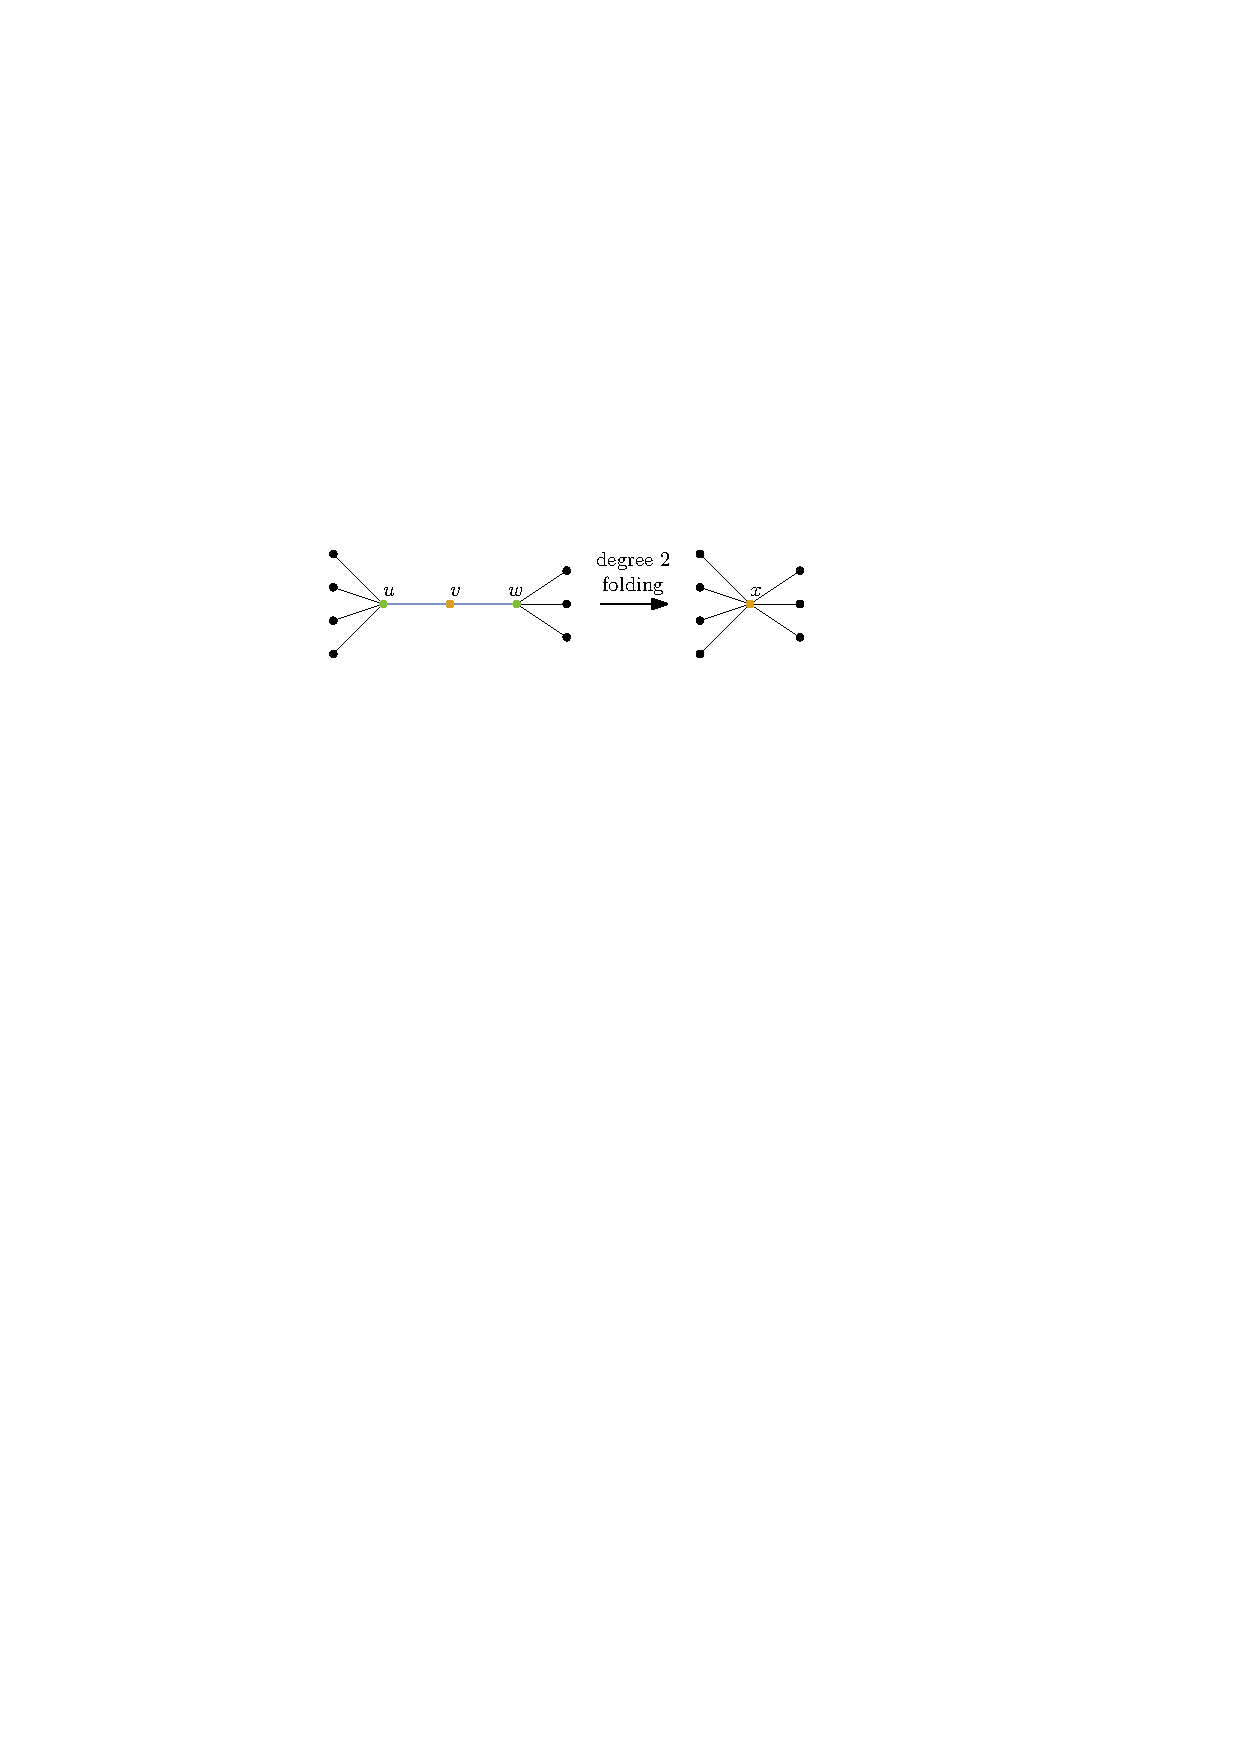
\includegraphics[scale=1.5]{images/deg2_red}
\centering
\caption{Degree two folding: vertices $u$, $v$ and $w$ are replaced with a single vertex $x$. The remaining neighbors of $u$ and $w$ are connected to $x$.}
\label{fig:dg2}
\end{figure}
\paragraph{}
The next two reduction rules can be used to delete single vertices that are not required in a maximum independent set. The first of those rules (the dominance reduction) is fully contained in the second rule (the unconfined reduction) and therefore the algorithm only uses the latter one. However, we used the concept of dominance to design one of our branching strategies. For this reason the dominance reduction rule proposed by Fomin et al. \cite{Fomin} is also featured in detail.

\begin{definition} (Dominance)
	In a graph $G=(V,E)$ a vertex $u$ is called dominated by a neighbor $v$, if $N[u]\subseteq N[v]$.
\end{definition}


\begin{theorem} (Dominance Reduction) In a graph $G=(V,E)$, if a vertex $u$ is dominated by a neighbor $v$, then, there always exists a maximum independent set that does not include $v$, i.e.\[\alpha(G)=\alpha(G-v)\]
\end{theorem}
\begin{proof}
	Consider a maximum independent set $I$ that does contain $v$. Since $N[u]\subseteq N[v]$, $I$ can neither contain $u$ nor any of its neighbors. But then, clearly, $I' = (I\setminus\{v\})\cup\{u\}$ is an \textit{independent set} of the same size as $I$ that does not include $v$.
\end{proof}
Thus, if a vertex $v$ dominates another vertex $u$, one could safely remove $v$ from the graph without compromising the solvabilty of the instance. This is illustrated in Figure \ref{fig:dom_red}.\\

\begin{figure}[htb]
	\captionsetup{belowskip=-1em}
	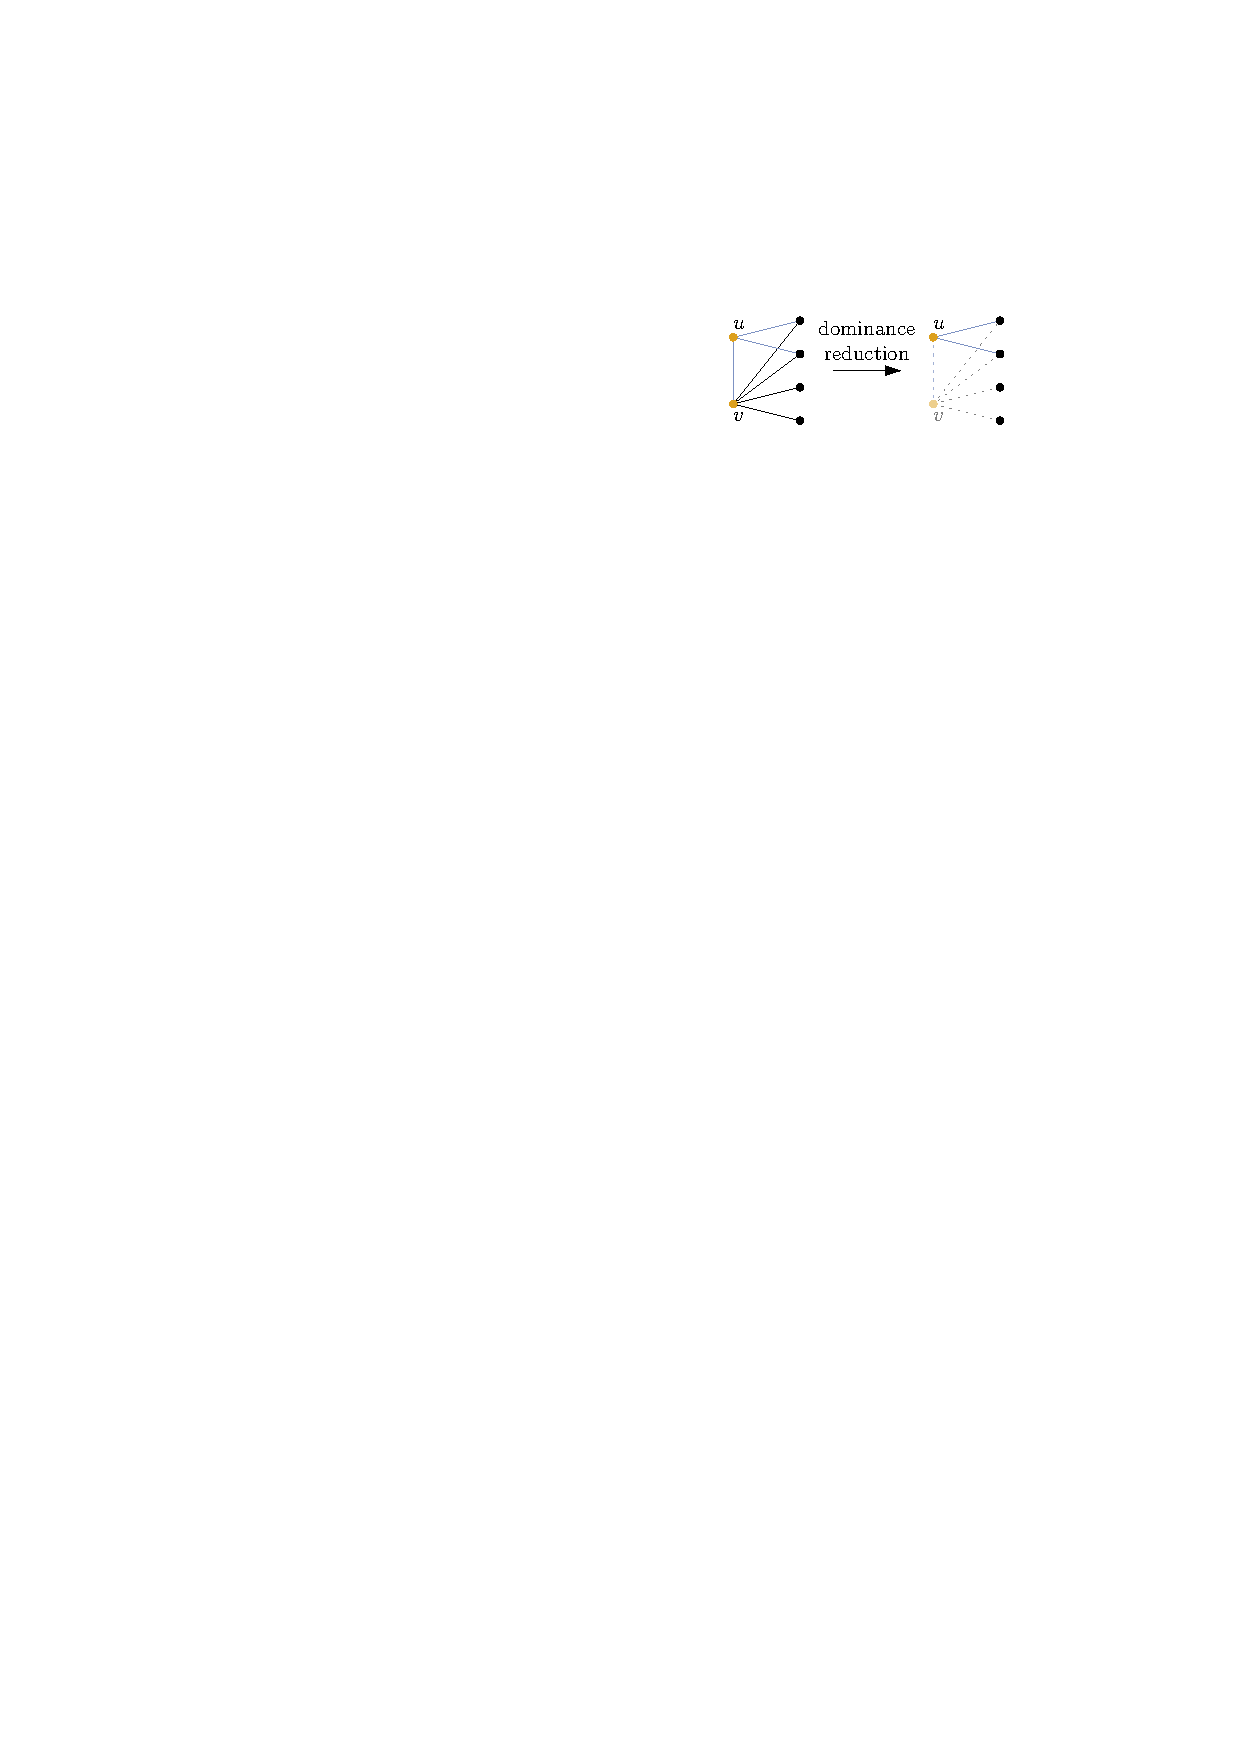
\includegraphics[scale=1.5]{images/dom_red}
	\centering
	\caption{Dominance reduction: vertex $u$ is dominated by vertex $v$. Thus, $v$ can be removed safely.}
	\label{fig:dom_red}
\end{figure}

\paragraph{}
The core idea of the \textit{unconfined reduction} proposed by Xiao and Nagamochi \cite{XiaoNagamochi} is to detect a vertex that is not required for a maximum independent set and therefore can be removed from the graph by algorithmically contradicting the assumption that every maximum independent set contains the vertex.

\begin{definition} (Removable Vertex)
	In a graph $G=(V,E)$ a vertex $v$ is called removable, if 
	\[\alpha(G) = \alpha(G-v)\]
\end{definition}

\begin{definition} (Child, Parent) In a graph $G=(V,E)$ with an \textit{independent set} $I$, a vertex $v$ is called a child of $I$, if $|N(v)\cap I| = 1$ and the unique neighbor of $v$ in $I$ is called the parent of $v$.
\end{definition}

\begin{theorem} \label{unconfined}
	In a graph $G=(V,E)$ let $S$ be an independent set that is not maximal but is contained in every maximum independent set of $G$ and let $v$ be any child of $S$. Then, every maximum independent set includes at least one vertex from $N(v)\setminus N[S]$.
\end{theorem}
\begin{proof}
	Assume that there is a maximum independent set $I$ that includes $S$ but no vertex from $N(v)\setminus N[S]$ and let $u$ be the parent of $v$ in $S$. Then, $I'=(I\setminus\{u\})\cup\{v\}$ is an independent set of the same size as $I$, since $I$ contains no neighbor of $v$ other than $u$. This contradicts the fact that every maximum independent set includes $S$.
\end{proof}

Based on Theorem \ref{unconfined} Algorithm \ref{alg:unconf} detects so called \textit{unconfined} vertices.

\begin{algorithm}
	\caption{Unconfined -- Xiao and Nagamochi \cite{XiaoUnconfined}}\label{alg:unconf}
	\SetKwFunction{U}{Unconfined}
	\DontPrintSemicolon
	
	\KwIn{A graph $G$, a vertex $v$}
	\U{G, v}	
	\Begin{
		$S \leftarrow \{v\}$\;
		\While{$S\text{ has child }u\text{ with } |N(u)\setminus N[S]|\leq 1$}{
			\eIf{$|N(u)\setminus N[S]| = 0$}{\Return true\tcp*{contradiction to Theorem \ref{unconfined}}}{
				$\{w\}\leftarrow N(u)\setminus N[v]$\tcp*{by assumption $w$ also has to}
				$S\leftarrow S\cup\{w\}$\tcp*{be contained in every MIS}
			}
		}
		
		\Return $\text{false}$
		
	}
	
	\KwOut{true if $v$ is unconfined, false otherwise}
	
\end{algorithm}


\begin{theorem}(Unconfined Reduction) In a graph $G=(V,E)$, if Algorithm \ref{alg:unconf} returns true for an unconfined vertex $v$, then there is always a maximum independent set that does not contain~$v$.
\end{theorem}
\begin{proof}
	Assume $v$ is included in every maximum independent set. Every vertex added to $S$ by the algorithm is the unique neighbor of a child of $S$. Therefore, by Theorem \ref{unconfined} this vertex also has to be contained in every maximum independent set, and thus can be added to $S$. If the algorithm returns true, then there is a child of $S$ that has no neighbor that can be included in $S$. Thus, by Theorem \ref{unconfined} the assumption that $v$ is included in every maximum independent set was false and therefore $v$ is removable.
\end{proof}
During kernelization the branch and reduce algorithm uses Algorithm \ref{alg:unconf} to detect and remove unconfined vertices.\paragraph{}
The twin reduction by Xiao and Nagamochi \cite{XiaoUnconfined} deals with pairs of degree three vertices that share the same neighborhood.

\begin{definition}(Twins)
	In a graph $G=(V,E)$ two vertices $u$ and $v$ are called twins, if $N(u) = N(v)$ and $d(u) = d(v) = 3$.
\end{definition}

\begin{theorem} (Twin Reduction) In a graph $G=(V,E)$ let vertices $u$ and $v$ be twins. If there is an edge among $N(u)$, then there is always a maximum independent set that includes $\{u,v\}$ and therefore excludes $N(u)$. Otherwise, let $G'=(V',E')$ be the graph with $V'=(V\setminus N[\{u,v\}])\cup\{w\}$ where $w\notin V$ and $E'=(E\cap\binom{V'}{2})\cup \{\{w,x\}\;|\;x\in N^2(u)\})\}$ and let $I'$ be a \textit{maximum vertex cover} in $G'$. Then, 
	
	\[I=\begin{dcases}
	I'\cup \{u,v\} & \text{, if }w\notin I'\\
	(I'\setminus \{w\})\cup N(u) & \text{, else} %w\in I'
	\end{dcases}\]
	is a maximum independent set in $G$.
\end{theorem}
\begin{proof}
	For the first case, i.e., there is an edge among $N(u)$, consider a maximum independent set $I$ that does not contain $u$ or $v$. Then, $I$ has to include at least one neighbor of $u$ and $v$, because otherwise $I\cup \{u,v\}$ would be an \textit{independent set} larger than $I$. On the other hand, since there are neighbors of $u$ and $v$ that are adjacent, $I$ can only contain at most two neighbors of $u$ and $v$. But then, $I' = (I\setminus N(u))\cup\{u,v\}$ is an \textit{independent set} of the same size as I that includes $u$ and $v$. For the second case, i.e., there are no edges among $N(u)$, note that the reduction produces a set which in both cases contains exactly two vertices more than a maximum independent set in $G'$. Now consider a maximum independent set $I$ in $G$. If $N(u)$ is completely contained in $I$ ($N(U)\subseteq I$), then $I$ can not contain any vertex of $N^2(u)$, i.e., any neighbor of $w$ in $G'$. Thus, $I' = (I\setminus N(u))\cup\{w\}$ is an \textit{independent set} of $G'$ of size $|I| - 2$. Otherwise, $I$ contains at most two vertices from $N(u)\cup\{u,v\}$ (either $u$ and $v$ or two vertices from $N(u)$). But then, $I' = I\setminus(N(u)\cup\{u,v\})$ is also an \textit{independent set} of $G'$ of size $|I|-2$. In total $\alpha(G) \leq \alpha(G')+2$ and thus, $I$ is a maximum independent set of $G$
\end{proof}

During the kernelization step the algorithm searches for twins $u$ and $v$. If there is an edge among $N(u)$, the algorithm includes $u$ and $v$ to the current solution and deletes $\{u,v\}\cup N(u)$. Otherwise, the algorithm still deletes $\{u,v\}\cup N(u)$ introducing a new vertex connected to $N(u)\setminus\{u,v\}$ instead. Both cases of the twin reduction are depicted in Figure \ref{fig:twin_red}.\\

\begin{figure}[htb]
	\centering
	\captionsetup[subfigure]{aboveskip=1em,belowskip=1em}
	\captionsetup{belowskip=-1em, aboveskip=0em}
	\begin{subfigure}{\textwidth}
		\centering
		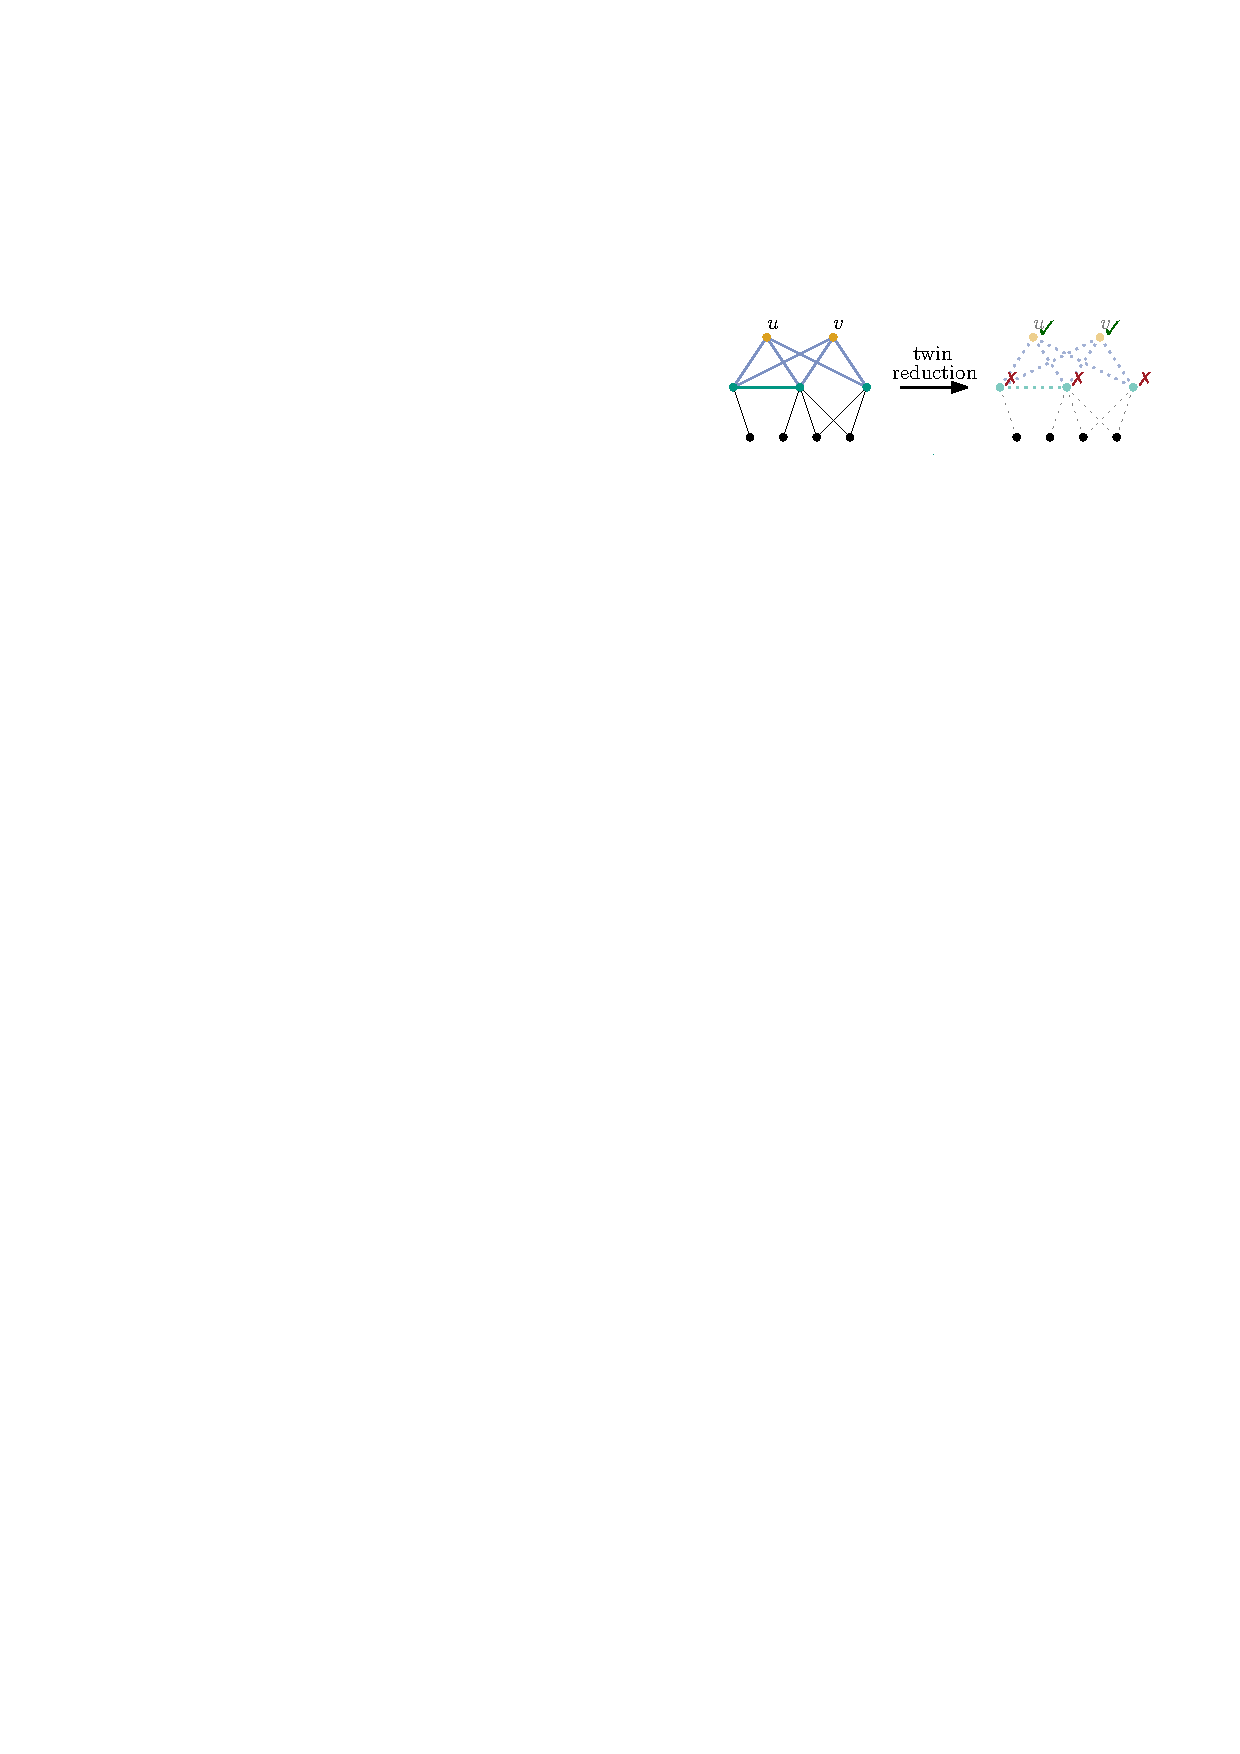
\includegraphics[scale=1.5]{images/twin_red_2}
		\caption{Case one: there is an edge between any two neighbors of $u$ and $v$. Thus, the neighborhood of $u$ and $v$ is excluded from the current independent set, whereas $u$ and $v$ are included into the current independent set.}
	\end{subfigure}
	%\subfloat[][a]{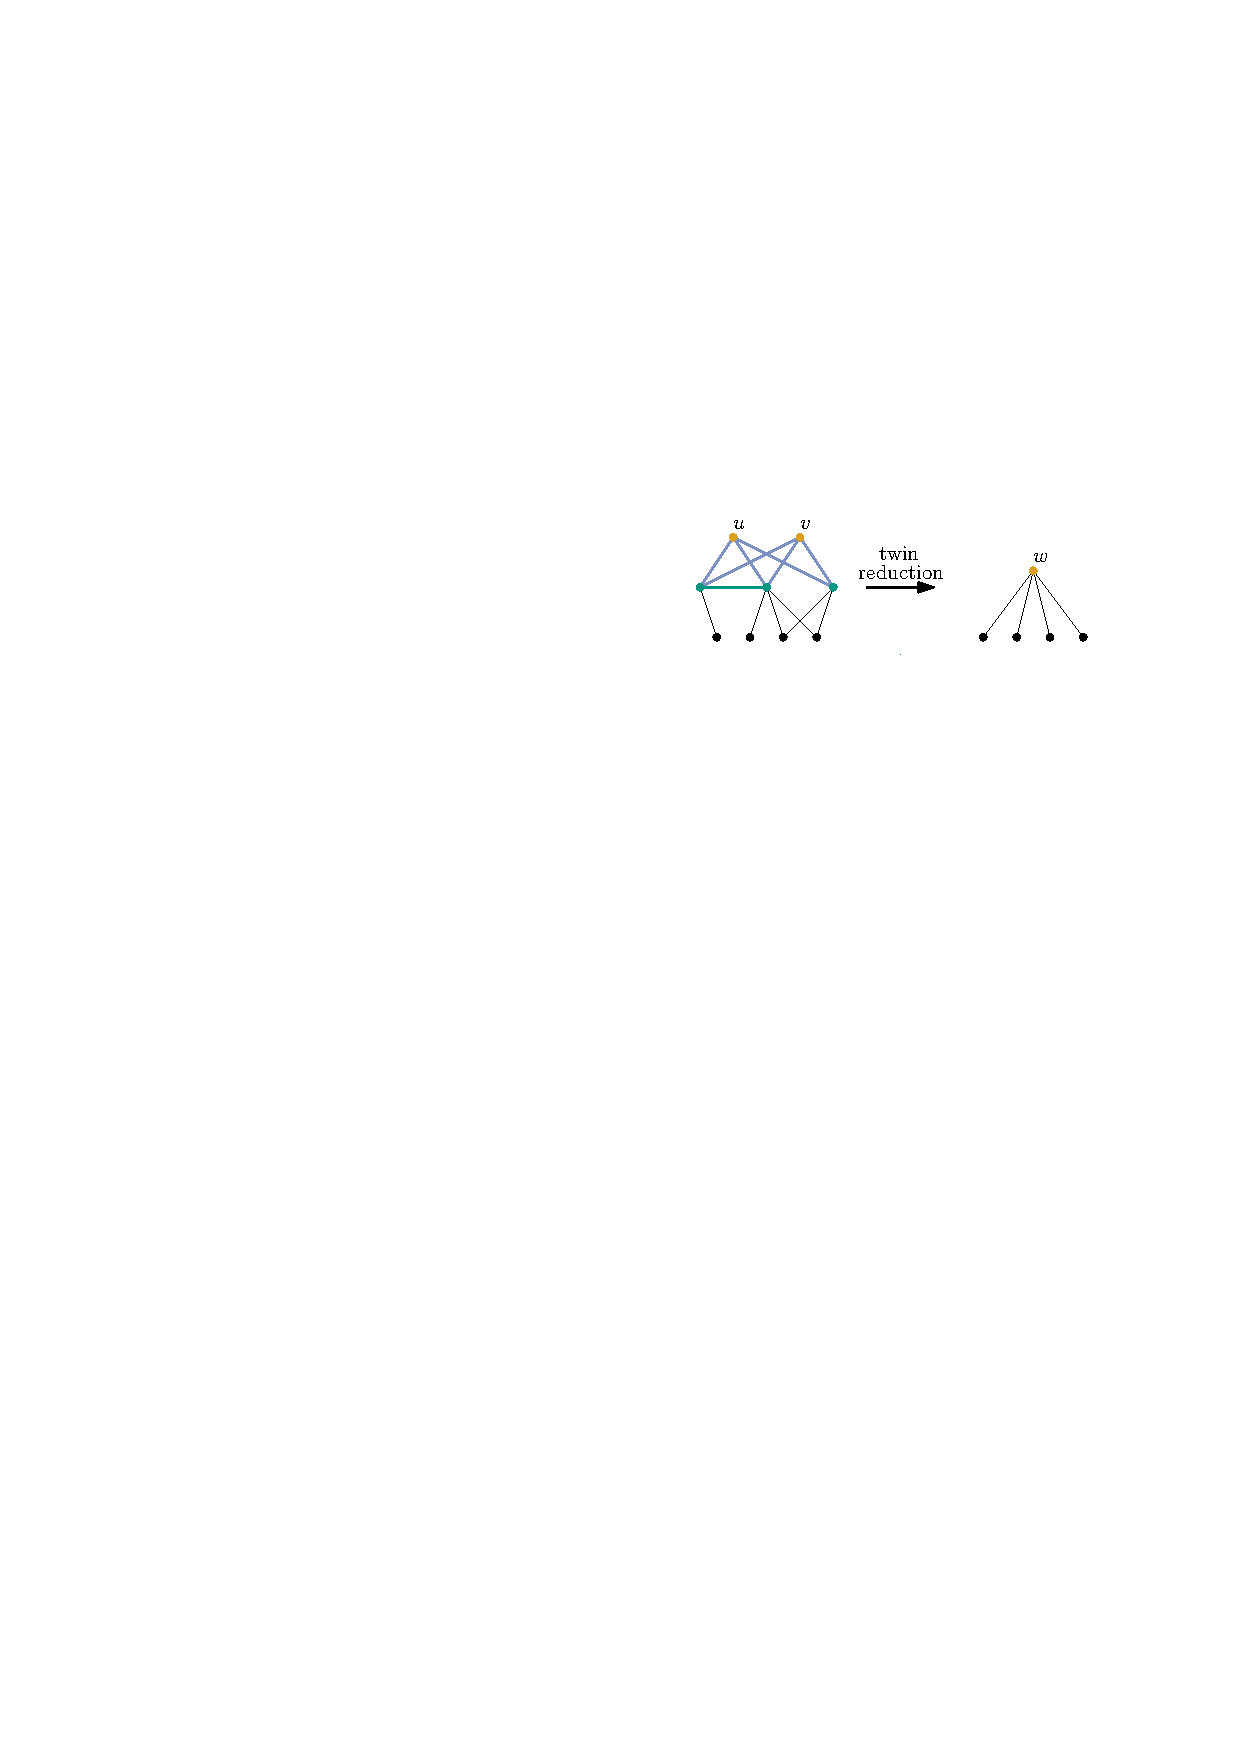
\includegraphics[width=\textwidth]{images/twin_red_1}}
	\begin{subfigure}{\textwidth}
		\centering
		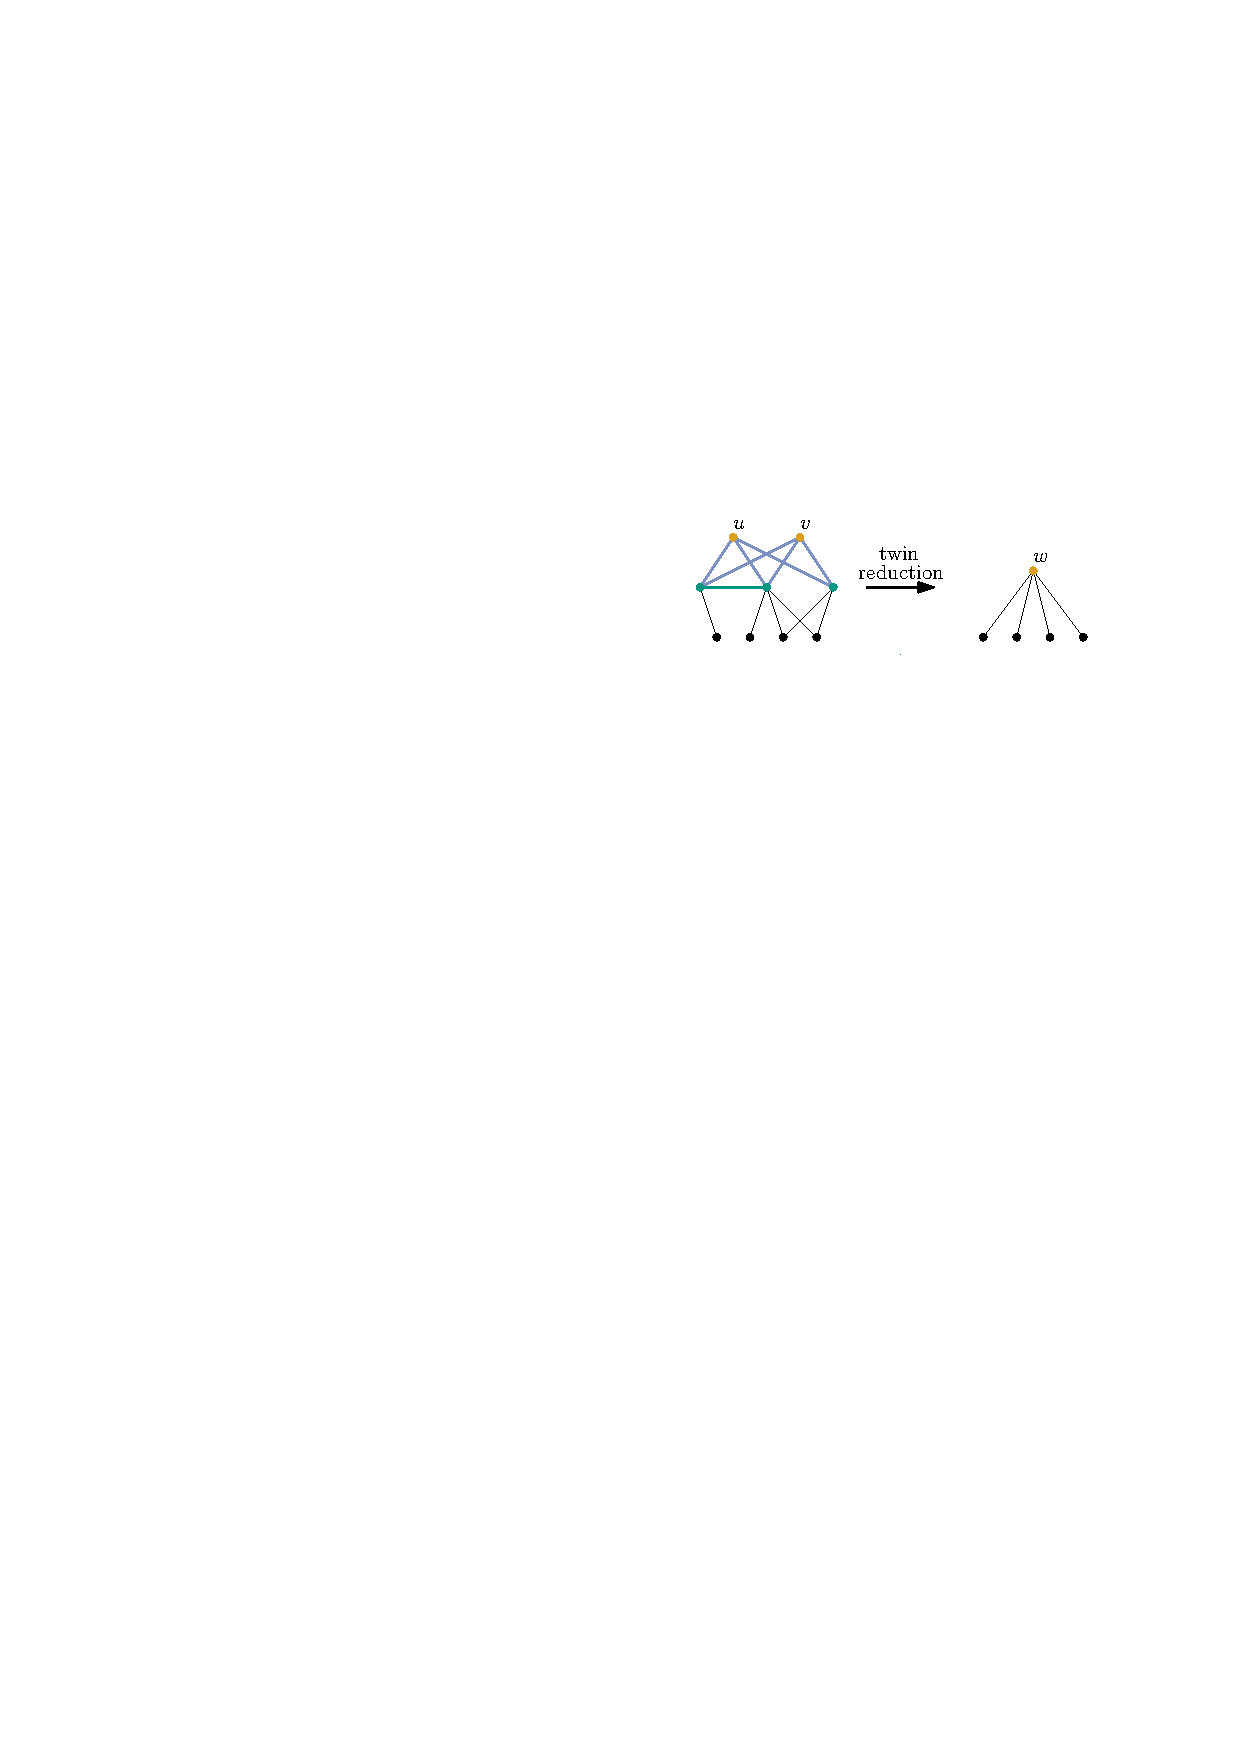
\includegraphics[scale=1.5]{images/twin_red_1}
		\caption{Case two: there are no edges between neighbors of $u$ and $v$. Thus, $u$, $v$ and the neighborhood of $u$ and $v$ are replaced with a single vertex $w$. Each vertex from $N^2(v)$ is connected to $w$.}
	\end{subfigure}
\caption{Twin reduction: vertices $u$ and $v$ are twins}
\label{fig:twin_red}
\end{figure}

\paragraph{}
The next reduction rule as well as its featured special cases are also proposed by Xiao and Nagamochi~\cite{XiaoUnconfined}.

\begin{definition} (Alternative Sets)
	In a graph $G=(V,E)$ two non empty, disjoint subsets $A,B\subseteq V$ are called alternatives, if $|A| = |B|$ and there is a maximum independent set $I$ in $G$ such that $I\cap(A\cup B)$ is either $A$ or $B$.
\end{definition}
\begin{theorem} (Alternative Reduction)
	In a graph $G=(V,E)$ let $A$ and $B$ be alternative sets. Let $G'=(V', E')$ the graph with $V' = V\setminus(A\cup B\cup (N(A)\cap N(B)))$ and $E' = (E\setminus\binom{A\cup B\cup (N(A)\cap N(B))}{2} \cup \{ \{x,y\}\;|\; x\in N(A)\setminus N[B], y\in N[B]\setminus N(A) \}$ and let $I'$ be a maximum independent set in $G'$. Then,
	
	\[I=\begin{dcases}
	I'\cup A & \text{, if } (N(A)\setminus N[B]) \cap I' = \emptyset% N(B)\setminus N[A]\subseteq I'\\
	\\
	I'\cup B & \text{, else if } (N(B)\setminus N[A])\cap I' = \emptyset
	\end{dcases}\]
	is a maximum independent set in $G$.
\end{theorem}
\begin{proof}
	Consider a maximum independent set $I$ in $G$ and without loss of generality let $A\subseteq I$ (by definition $A$ or $B \subseteq I$). Thus, $I\cap ((A\cup B\cup (N(A)\cap N(B))) = A$ and $I\cap(N(A)\setminus N[B])=\emptyset$. Now let $I' = I\setminus A$. $I'$ is an \textit{independent set} in $G'$, since each added edge (from $E'\setminus E$) is incident to a vertex from $N(A)\setminus N[B]$ and also $|I'| = |I|-|A|$. This implies $\alpha(G')+|A| \geq \alpha(G)$.
	
	Conversely, let $I'$ be a maximum independent set of $G'$. Obviously, $I'$ is also an \textit{independent set} of $G$. Since vertices from $N(A)\setminus N[B]$ are pairwise adjacent to vertices form $N(B)\setminus N[A]$, $I'$ can only contain vertices from either $N(A)\setminus N[B]$ or $N(B)\setminus N[A]$. But then, $I=I'\cup A$ or $I=I'\cup B$, respectively, is an \textit{independent set} in $G$. Thus, $\alpha(G')+|A| \leq \alpha(G)$
	In total $\alpha(G')+|A| = \alpha(G)$ and $I$ is a maximum independent set in $G$.
\end{proof}
Note that the \textit{alternative reduction} adds new edges between existing vertices of the graph. For this reason, applying the \textit{alternative reduction} is not beneficial in every case. To counteract this, the algorithm only uses the following special cases of the \textit{alternative reduction}.

\begin{definition} (Funnel)
	In a graph $G=(V,E)$ two adjacent vertices $u$ and $v$ are called funnels, if $G_{N(v)\setminus\{u\}}$ is a complete graph, i.e, if $N(v)\setminus\{u\}$ is a clique.
\end{definition}
\begin{theorem} (Funnel Reduction) In a graph $G=(V,E)$ let $u$ and $v$ be funnels. Then, $\{u\}$ and $\{v\}$ are alternative sets.	
\end{theorem}
\begin{proof}
	We have to show that there is a maximum independent set that contains either $v$ or $u$. So, consider a maximum independent set $I$ that excludes both $u$ and $v$. Then, $I$ has to include at least one vertex from $N(v)\setminus\{u\}$, because otherwise $I\cup\{v\}$ would be an \textit{independent set} of larger size. On the other hand, $I$ can only contain at most one vertex $x$ from $N(v)\setminus\{u\}$, since $N(v)\setminus\{u\}$ is a clique. But then $(I\setminus\{x\})\cup\{v\}$ is an \textit{independent set} of the same size as $I$ that does contain $v$. Thus $\{u\}$ and $\{v\}$ are alternative sets.
\end{proof}

\begin{definition} (Desk)
	In a graph $G=(V,E)$ a cycle $u_1u_2u_3u_4$ of length four with no chords (i.e., an induced 4-cycle) is called a desk, if each of the vertices has at least degree three, $N(\{u_1, u_3\})\cap N(\{u_2, u_4\}) = \emptyset$ and $|N(\{u_1, u_3\})\setminus \{u_2, u_4\}|\leq 2$ as well as $|N(\{u_2, u_4\})\setminus \{u_1, u_3\}|\leq 2$.
\end{definition}
\begin{theorem}(Desk Reduction) 
	In a graph $G=(V,E)$ let $u_1u_2u_3u_4$ be a desk. Then $\{u_1, u_3\}$ and $\{u_2, u_4\}$ are alternative sets.	
\end{theorem}
\begin{proof}
	Consider a maximum independent set $I$ of $G$. If $|I\cap \{u_1,u_2,u_3,u_4\}| > 1$, then clearly\\ $I\cap \{u_1,u_2,u_3,u_4\} $ is either $\{u_1, u_3\}$ or $\{u_2, u_4\}$. Otherwise, without loss of generality $u_2,u_3,u_4\notin I$ and $|I\cap N[\{u_1,u_3\}]|=2$. The last equation holds because $|N(\{u_1, u_3\})\setminus\{u_2,u_4\}| \leq 2$ by definition, and $u_1$ has at least one neighbor in $N(\{u_1, u_3\})\setminus\{u_2,u_4\}$ ($d(u_1)\geq3$). But then $(I\setminus\{N(\{u_1,u_3\})\})\cup\{u_1,u_3\}$ is an \text{independent set} of the same size as $I$ that does contain $\{u_1, u_3\}$. Thus, $\{u_1,u_3\}$ and $\{u_2, u_4\}$ are alternative sets.
\end{proof}

During kernelization the algorithm searches for funnels or desks and reduces those structures according to the alternative reduction. Examples for structures which admit funnel or desk reduction, respectively, are illustrated in Figure \ref{fig:funnel_red} and \ref{fig:desk_red}.


\begin{figure}[htb]
	\captionsetup{belowskip=0em}
	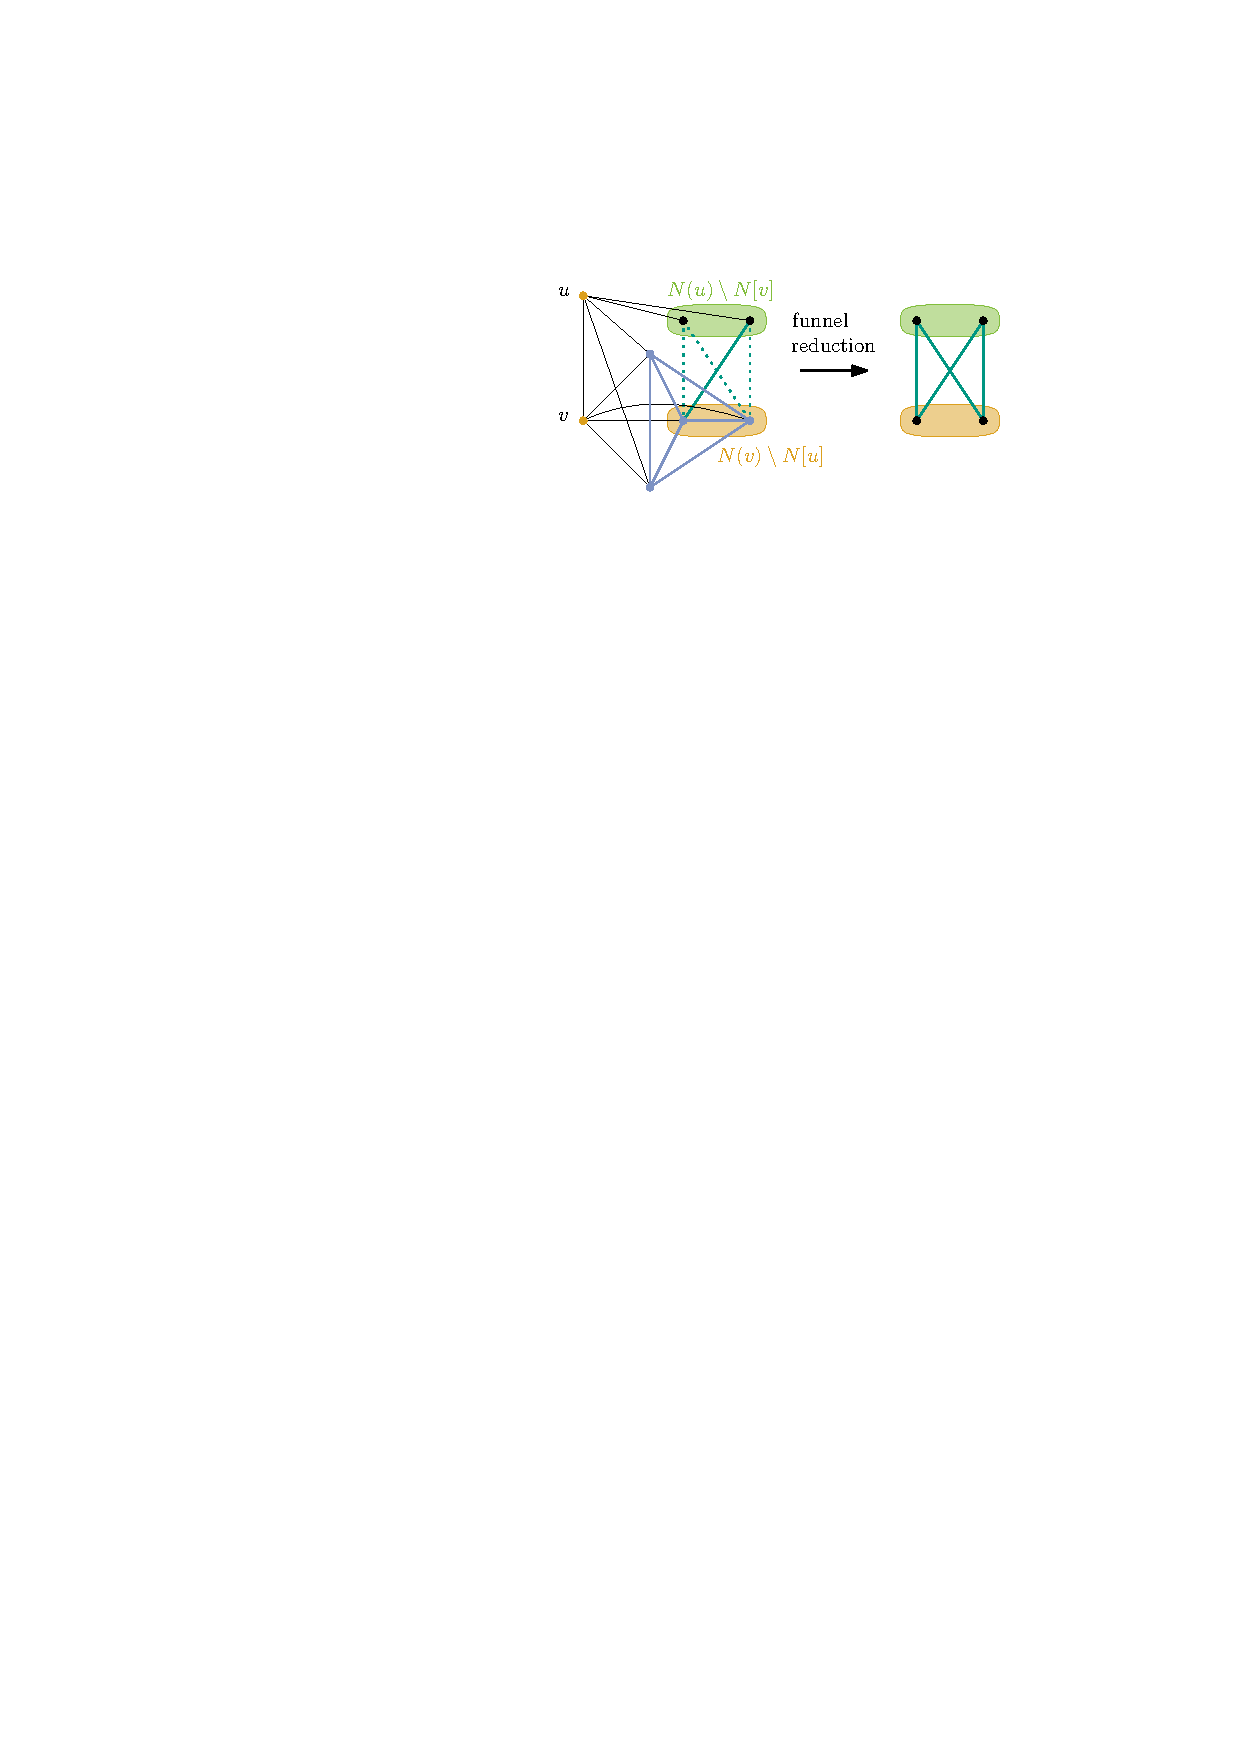
\includegraphics[scale=1.5]{images/funnel_red}
	\centering
	\caption{Funnel reduction: vertices $u$ and $v$ are funnels. The clique induced by $N(v)\setminus\{u\}$ is highlighted in blue. The vertices $u$, $v$ and their common neighborhood ($N(u)\cap N(v)$) are removed from the graph. Vertices from $N(u)\setminus N[v]$ are pairwise connected to the vertices from $N(v)\setminus N[u]$.}
	\label{fig:funnel_red}
\end{figure}

\begin{figure}[htb]
	\captionsetup{belowskip=-1em}
	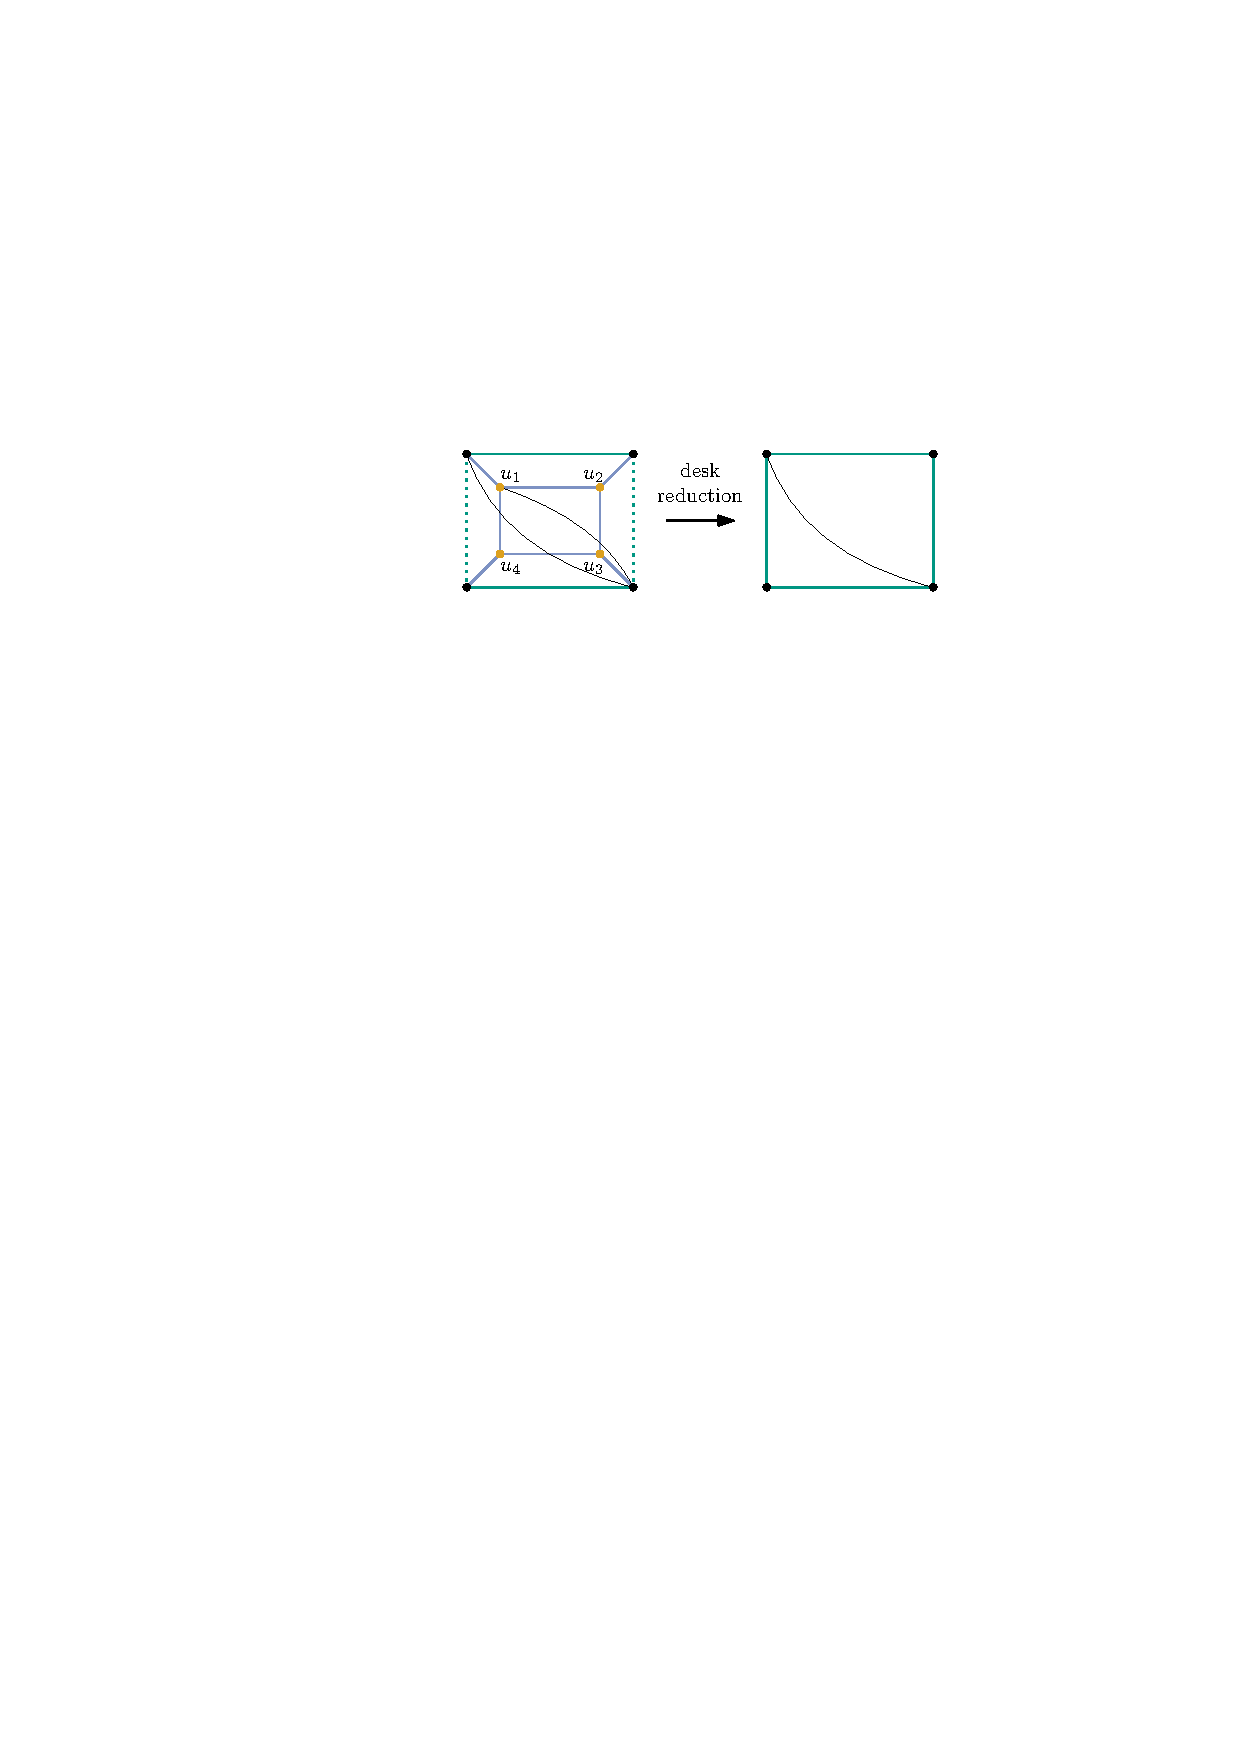
\includegraphics[scale=1.5]{images/desk_red}
	\centering
	\caption{Desk reduction: vertices $u_1$, $u_2$, $u_3$ and $u_4$ form a desk structure. Thus, they are removed from the graph and vertices from $N(\{u_1,u_3\})\setminus N[\{u_2,u_4\}]$ are pairwise connected to the vertices from $N(\{u_2,u_4\})\setminus N[\{u_1,u_3\}]$. }
	\label{fig:desk_red}
\end{figure}

\paragraph{}
The algorithm also uses a reduction based on a solution to the LP-Relaxation of maximum independent set.
\begin{gather*}
\text{maximize} \sum_{v\in V}x_v\\
0\leq x_v\leq 1 \;\;\; \forall v\in V\\
x_v + x_u\leq 1 \;\;\; \forall \{u,v\}\in E
\end{gather*}

Nemhauser and Trotter \cite{NemhauserTrotter} show that there always exists an optimal half integral solution to the LP-Relaxation, i.e., an optimal solution where $x_v\in\{0,\frac{1}{2},1\}$ for all $v\in V$. They also show that given an optimal half integral solution to the LP-Relaxation, there is always a maximum independent set that includes all vertices $v$ with $x_v=1$ and excludes all vertices $u$ with $x_u = 0$. Furthermore, they show that finding an optimal half integral solution can be reduced to computing a \textit{maximum matching} in a bipartite graph. Iwata et al. \cite{IwataOkaYoshida} propose an algorithm that given any optimal half integral solution constructs another half integral solution that minimizes the number of variables with half integral value in linear time. The branch and reduce algorithm uses this solution to the LP-Relaxation to reduce the graph and also as an upper bound to an optimal solution.\paragraph{}
Apart from reduction rules, the algorithm also uses branching rules that allow further reductions on branching when certain conditions hold. The first branching rule, mirror branching, is introduced by Fomin et al. \cite{Fomin}. According to Kneis et al. \cite{Kneis} it is potentially useful, if the branching vertex has a rather low degree and thus, most likely has some mirror.

\begin{definition} (Mirror)
	In a graph $G=(V,E)$ a vertex $u$ is called a mirror of a vertex $v$, if $u\in N^2(v)$ and $G_{N(v)\setminus N(u)}$ is a (possibly empty) complete graph, i.e. $N(v)\setminus N(u)$ is a (possibly empty) clique. The set of all mirrors of $v$ is denoted by $\mathcal{M}(v)$ and $\mathcal{M}[v] := \mathcal{M}(v)\cup\{v\}$.
\end{definition} 
\begin{theorem} (Mirror Branching)
	In a graph $G=(V,E)$, if there is no maximum independent set that contains a vertex $v$, then every maximum independent set also excludes $\mathcal{M}[v]$.
\end{theorem}
\begin{proof}
	Consider any maximum independent set $I$ of $G$. Then $I$ has to contain at least two neighbors of $v$ because otherwise, we could get a maximum independent set $I'=(I\setminus N(v))\cup\{v\}$ that includes $v$. Now let $u\in\mathcal{M}(v)$ be a mirror of $v$. Since $N(v)\setminus N(u)$ is a clique, $I$ can only contain at most one vertex from $N(v)\setminus N(u)$. Thus, $I$ contains at least another vertex from $N(v)\cap N(u)$ and therefore has to exclude $u$.
\end{proof}

So, when branching on a vertex $v$, the algorithm finds its mirrors $\mathcal{M}(v)$ and considers two possible cases. The first cases is that there is a maximum independent set that includes $v$ and therefore excludes $N(v)$. The second case is that no maximum independent set includes $v$. In this case, the vertices from $\mathcal{M}(v)$ can also be discarded from the graph.

\begin{figure}[htb]
	\captionsetup{belowskip=-1em}
	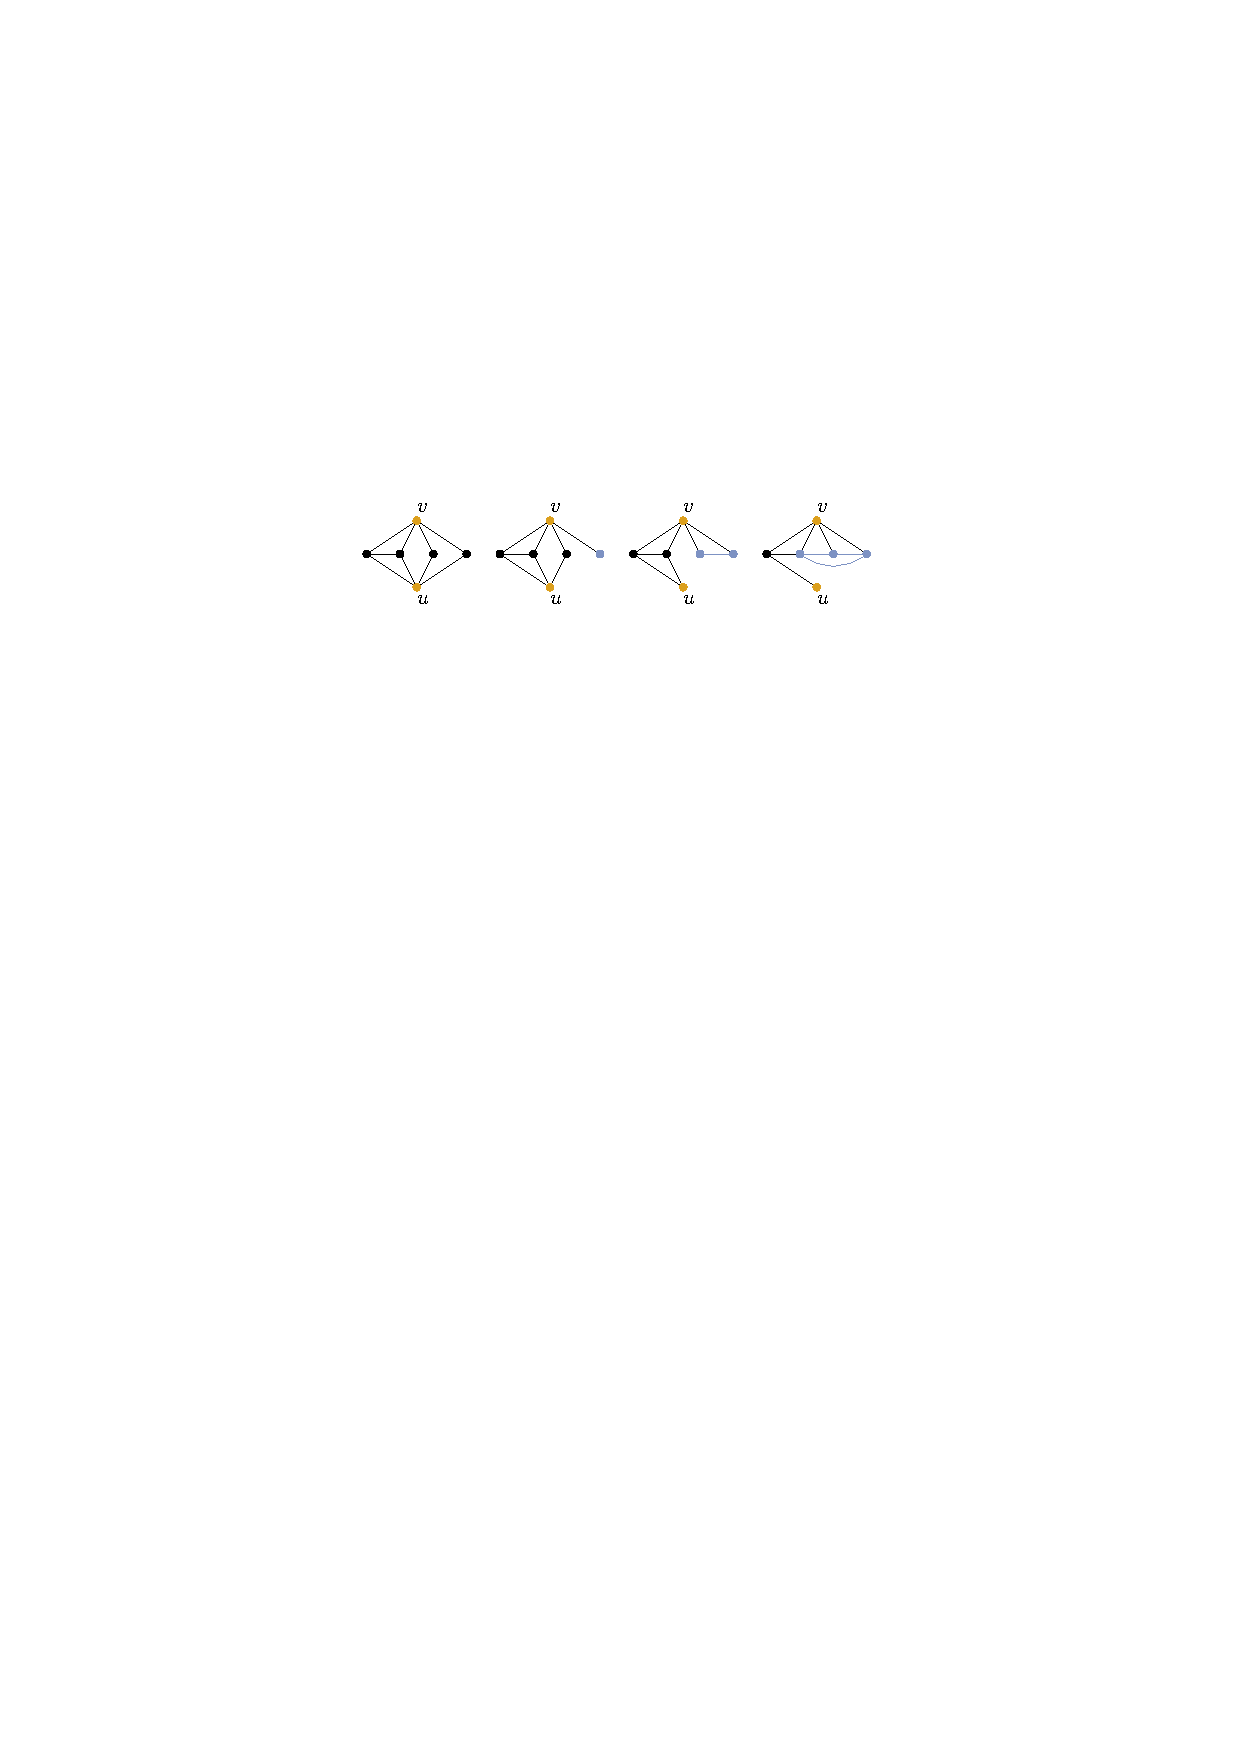
\includegraphics[scale=1.5]{images/mirror}
	\centering
	\caption{Mirror branching: vertex $u$ is a mirror of $v$. The possibly empty clique induced by $N(v)\setminus N(u)$ is highlighted in blue. When either $u$ or $v$ is excluded from the current independent set by branching, the other vertex is also discarded. }
	\label{fig:mirror}
\end{figure}

\paragraph{}
The packing branching rule by Akiba and Iwata \cite{AkibaIwata} is a generalization of the idea behind the satellite branching rule by Kneis et al. \cite{Kneis}. The core idea behind those rules is that when branching in the case of excluding a vertex $v$ from the solution, one can assume that no maximum independent set contains $v$. Otherwise, if there is a maximum independent set that contains $v$, the algorithm finds it in the branch that includes $v$. Based on the assumption that no maximum independent set includes a vertex $v$, constraints for the remaining vertices can be derived. For example, a maximum independent set that does not contain $v$ has to include at least two neighbors of $v$. The corresponding constraint is $\sum_{u\in N(v)}x_u \geq2$, where $x_u$ is a binary variable that indicates whether a vertex is included in the current solution. The algorithm creates such constraints when branching, and updates them accordingly during the kernelization and branching steps. The constraints can then be used to reduce the graph or to prune the current branch when a constraint can not be fulfilled by the current solution.

\clearpage

%%%%%%%%%%%%%%%%%%%%%%%%%%%%%%%%%%%%%%%%%%%%%%%%%%%%%%%%%%%%%%%%%%%%%%

\section{Related Work} \label{sec3}

This section discusses related work. It focuses on presenting branching strategies used by other branch and reduce algorithms for maximum independent set or its equivalent problems minimum vertex cover and maximum clique.

\paragraph{}
There are various approaches to tackle the maximum independent set problem and its equivalent problems. These approaches comprise exact as well as heuristic methods. A technique frequently used for both exact and inexact algorithms is kernelization. We already covered the most important reduction rules used for kernelization in Section \ref{sec2}.

\paragraph{}
Due to the NP-Hardness of the maximum independent set problem, inexact algorithms have been well studied. One of the best techniques used for finding large independent sets is local search~\cite{ARW, NUMVC}. Local search algorithms start with an initial solution and then utilize simple operations to iteratively improve the current solution. In practice, local search algorithms often find near optimal solutions very fast. However, most of them can not give any guarantee for the actual quality of a solution. One of the best local search algorithms for maximum independent set, called ARW, is proposed by Andrade et al.~\cite{ARW}. Their algorithm uses the concept of $(j,k)$-swaps, i.e., removing $j$ vertices from the current solution and replacing them with $k$ vertices instead. In every iteration of their algorithm, they perform a $(1,2)$-swap to improve the current solution. A valid $(1,2)$-swap can be found in linear time. To escape local optima, ARW occasionally disturbs the current solution by randomly inserting vertices into it and removing their neighbors instead.

\paragraph{}
Chang et al.~\cite{ChangKern} propose a linear time kernelization algorithm which reduces vertices of degree one and two. In fact, Strash \cite{Strash} shows that using those simple reduction rules alone is sufficient to solve many real-world instances. Another variant of their algorithm, called NearLinear, additionally applies the dominance and LP reduction rule, but has only near-linear runtime. The authors also show that applying their kernelization algorithm iteratively followed by removing vertices of high degree, results in a large initial solution which, in turn, speeds up the ARW local search algorithm.
\paragraph{}
The most powerful exact exponential time algorithms for maximum independent set are, on a theoretical basis, branch and reduce algorithms \cite{XiaoNagamochi, ChenXiaKanj}. These algorithms use kernelization to compute a kernel of the input instance. After that they branch into subinstances with lower complexity which are then solved recursively. We now discuss the branching strategies used in various different branch and reduce algorithms.

\paragraph{}
The most common branching strategy used for maximum independent set and minimum vertex cover is branching on a vertex of maximum degree. Fomin et al. \cite{Fomin} give a theoretical analysis of this using the measure and conquer technique with a weighted degree sum as measure. The authors show that choosing a vertex of maximum degree that also minimizes the number of edges in its neighborhood is optimal with respect to their complexity measure. This greedy strategy is also used by the algorithm of Akiba and Iwata \cite{AkibaIwata} and serves as a baseline for comparison in our experiments. Akiba and Iwata already compare this strategy with branching on a vertex of minimum degree and the strategy of choosing a branching vertex at random. Their experiments show that those strategies are significantly worse than branching on maximum degree vertices.

\paragraph{}
Xiao and Nagamochi \cite{XiaoNagamochi} propose a branch and reduce algorithm for maximum independent set that, in most cases, branches on a vertex of maximum degree but also uses a special edge branching strategy to handle dense subgraphs. Edge branching is based on the principle of alternative subsets like in alternative reduction. Given an edge $\{u,v\}\in E$ a maximum independent set can only contain $u$ or $v$ but not both of them. So, if there is a maximum independet set that includes $u$ or $v$, then $\{u\}$ and $\{v\}$ are alternative sets. Thus, branching on the edge $\{u,v\}\in E$ yields two cases. The first case is to remove both $u$ and $v$ and to search for a maximum independent set that does not include $u$ and $v$. The second case is to compute the alternative reduction of $\{u\}$ and $\{v\}$, i.e., to remove $\{u,v\}\cup(N(u)\cap N(v))$ and insert an edge $\{x,y\}$ between any nonadjacent vertices $x\in N(u)\setminus N(v)$ and $y\in N(v)\setminus N[u]$ and to search for a maximum independent set that includes either $u$ or $v$.

The algorithm by Xiao and Nagamochi uses edge branching in degree bounded graphs on edges $\{u,v\}\in E$, where $|N(u)\cap N(v)|$ is sufficiently large, i.e., the concrete values depend on the maximum degree of the graph. 

\paragraph{}
Bourgeois et al. \cite{Bourgeois} present a branch and reduce algorithm for maximum independent set that relies on fast algorithms for graphs with low average degree. If the average degree of the graph is greater than 4, the algorithm branches on a vertex of maximum degree. Otherwise, if the average degree of the graph is at most 4, they use a specialized algorithm to solve the instance. If there is no vertex with degree of at least 5, this algorithm branches on vertices contained in 3- or 4-cycles.

\paragraph{}
Chen, Kanj and Xia \cite{ChenXiaKanj} propose a branch and reduce algorithm for the problem minimum vertex cover parameterized by the size $k$ of the vertex cover, i.e., the problem of finding a vertex cover of size not larger than $k$. In their algorithm they use the concept of so called tuples and good pairs. A good pair is a pair of adjacent vertices that are advantageous for branching (the details are omitted here). A tuple is a set $S$ of vertices together with the number of vertices in $S$ that can be excluded from a minimum vertex cover. This information can be exploited during the branching to eliminate additional vertices. For example, consider the pair $(\{u,v\}, 1)$. We know that either $u$ or $v$ can be excluded from a minimum vertex cover and thus, if we include $u$ to the vertex cover, we can exclude $v$. Otherwise, if we exclude $u$ from the vertex cover, we can include $v$. Akiba and Iwata \cite{AkibaIwata} use the same idea in their packing reduction. The algorithm by Chen, Kanj and Xia maintains a set of these structures as well as vertices of high degree and updates them accordingly during kernelization and branching. At each branching step the algorithm chooses the best structure and branches on it.

\paragraph{}
Most branch and reduce algorithms for maximum clique use some sort of greedy coloring to find an upper bound to the size of a maximum clique and also to reduce the number of possible vertices for branching \cite{Color}. Given a coloring $c:V \rightarrow \mathbb{N}$ and the size $c_\text{max}$ of a current best solution, it is easy to see that for $A = \{v\in V \;|\; c(v)\leq c_\text{max}\}$, $G_A$ can not contain a clique larger than the current best solution. Thus, only vertices from $V\setminus A$ are considered for branching.
\paragraph{}
More sophisticated algorithms use a MaxSAT encoding of maximum clique to achieve better upper bounds and to further reduce the set of branching vertices \cite{LiFangXu,LiJiang}. Maximum clique can be reduced to MaxSAT by introducing a binary variable $x_v$ for every vertex $v\in V$ and a hard clause $\overline{x}_u\lor\overline{x}_v$ for each pair of non adjacent vertices. The set $\{x_v\;|\;v\in V\}$ of unit literals forms the soft clauses. A solution to this MaxSAT instance yields a maximum clique where the value of a variable indicates whether the corresponding vertex is included in the clique or not. A more efficient MaxSAT enconding of maximum clique is proposed by Li and Quan \cite{LiQuan}. Given a partition of $V$ into independent sets (i.e. a coloring), instead of introducing a soft clause for each vertex, they merely formulate a single clause $\bigvee_{x_i\in I_j} x_i$ for each independent set $I_j$ in the partition. Using this encoding they apply techniques from SAT solving like unit propagation and failed literal detection to identify conflicting independent sets. A set of $t$ independent sets is called conflicting if there is no clique of size $t$ in the subgraph induced by those independent sets. If conflicting independent sets are detected, the soft clauses get weakened by conjugating the clauses in a respective manner. The authors show that if a graph can be partitioned into $k$ independent sets with $t$ disjoint conflicting subsets, then the size of a maximum clique is bounded~by~$k-t$. This way, they achieve an upper bound which is often better than the bound obtained by the coloring.

\paragraph{}
Li et al. \cite{LiMaxSat} use a similar MaxSAT reasoning to reduce the number of vertices that are considered for branching. They initially use a coloring to obtain a partition of $V$ into parts $A$ and $V\setminus A$, where $A$ is defined as $A = \{v\in V \;|\; c(v)\leq c_\text{max}\}$ and $c_\text{max}$ is the size of the current best solution. After that they construct a MaxSAT instance where they add a soft clause for each color class (i.e. the set of vertices with the same color) in $A$. Then, they iteratively add a soft clause $x_{v_i}$ for each vertex $v_i \in V\setminus A$ and apply unit propagation to it. If a conflict is detected, the affected soft clauses get weakened. This process is repeated until no more conflicts are detected or $V\setminus A$ becomes empty. The authors show that if there are conflicts for literals $x_{v_1},\dots x_{v_k}$ with $v_i\in V\setminus A$, then the graph induced by $A\cup\{v_1\dots v_k\}$ does not contain a clique larger than the current best solution $c_\text{max}$. Thus, those vertices do not have to be considered for branching.

\paragraph{}
Another approach to decrease the number of branches in branch and reduce algorithms for maximum clique is to choose branching vertices in a specific beneficial order. A common strategy for choosing the branching vertex is to calculate a so called \textit{degeneracy ordering} $v_1 < v_2 < \dots < v_n$ where $v_i$ is a vertex of smallest degree in $G - \{v_1, \dots, v_{i-1} \}$, and to choose the vertices for branching in descending order \cite{CarraghanPardalos}. Li et al. \cite{LiFangXu} introduce another vertex ordering for branching using maximum independent sets. While $G$ is not empty, they repeatedly search for maximum independent sets and remove them from the graph. Then the vertex ordering is defined in the following way using the degeneracy ordering for tie breaking. For two vertices $u$ and $v$, $u < v$ if $u$ has been removed later than $v$ or if $u$ and $v$ have been removed at the same time but $u < v$ in the degeneracy ordering. 

\paragraph{}
Most of the exact algorithms for maximum independent set and its equivalent problems have been analyzed on a theoretical level but are not very well tested on real instances. In practice, the best algorithms use a combination of multiple techniques. For example, the winning solver of the PACE challenge by Hespe et al.~\cite{WGYC} uses kernelization, iterated local search, a branch and reduce algorithm for vertex cover and a branch and bound algorithm for maximum clique. Their algorithm starts by applying the same set of reduction rules as Akiba and Iwata \cite{AkibaIwata} do in their branch and reduce algorithm to obtain a kernel as small as possible. After that, they use iterated local search to find a large initial solution and prime the branch and reduce algorithm with it. Subsequently, the branch and reduce algorithm is run for a short period of time. If no solution is found during that time, they run a branch and bound maximum clique solver on the complement of kernel and, thereafter, on the complement of the original instance. Again, if no solution has been found so far, they re-run the branch and reduce algorithm for a longer time followed by the clique solver, if needed.

\clearpage
%%%%%%%%%%%%%%%%%%%%%%%%%%%%%%%%%%%%%%%%%%%%%%%%%%%%%%%%%%%%%%%%%%%%%%

\section{Branching Strategies} \label{sec4}
In this section we outline our approaches for designing the different branching strategies. We also give the details on the implementation itself and on the observations we made during the implementation. As mentioned in the introduction, we follow two main approaches in designing our branching strategies. 
\paragraph{}
The first approach is to decompose the graph by branching. This way, the resulting connected components can be solved independently speeding up kernelization and, potentially, reducing the total size of the search space. For this thesis we implemented three branching strategies using this approach which are described in Section \ref{decomp}.
\paragraph{}
The second approach is to break up complex structures that can not be reduced by kernelization. Our main idea behind this approach is to identify vertices that prevent a certain reduction rule from being applicable, and subsequently branch on them. This way, the respective reduction rule can be applied afterwards, and the graph gets further reduced. Also, such vertices can be found during kernelization which is continuously performed before every branching step. Therefore, the overhead of those branching strategies is rather small compared to the strategies following our first approach. We implemented branching strategies that target four different reduction rules and also tested a combination of those; branching strategies following this approach are covered in section \ref{red_strats}.
\paragraph{}

For almost all of our branching strategies it is not guaranteed that they find a suitable vertex for branching in every branching step. Consequently, all of them use a default branching strategy as a fallback. In our implementation we used branching on a vertex with maximum degree that also minimizes the number of edges among its neighborhood  as default branching strategy. This corresponds to the strategy proposed by Fomin et al. \cite{Fomin}, and is already implemented in the algorithm by Akiba and Iwata \cite{AkibaIwata}.

\subsection{Branching Strategies Based on Decomposition} \label{decomp}
\subsubsection{Branching on Articulation Points}
Since the branch and reduce algorithm, which we used as our basis, was designed for branching on a single vertex, our first idea is to find articulation points (i.e. cut vertices) of the graph and to branch on them. Articulation points of a graph $G$ are single vertices that form a separator of size one in $G$. Hence, by removing an articulation point the graph becomes disconnected. Given any spanning tree of $G$, each articulation point $v$ separates the vertices in the subtree rooted by a child of $v$ from the rest of the graph. Thus, in a spanning tree obtained by a depth first search (DFS) there are no back edges from the graph induced by the subtree rooted at this child to the predecessors of $v$ in the DFS tree.

\paragraph{}
Using this observation, articulation points in a connected graph can be found in linear time using the following algorithm (Algorithm \ref{alg:artic}) based on a depth first search scheme. The algorithm performs a depth first search starting at an arbitrary vertex of the graph. In every step of the DFS, the visited vertex is labeled with the current DFS number. If a back edge is found during the DFS run, the label of the currently visited vertex is updated to the minimum of the labels of both endpoints of the back edge. After the child of a vertex has been scanned by the DFS, the algorithm checks whether there were any back edges from the subtree rooted at the child to a predecessor of the vertex in the DFS tree. This is the case, if the label of the child is not smaller than the current label of the vertex. If there are no such back edges, then the current vertex is an articulation point. Eventually, the algorithm has to consider a special case for the root of the DFS tree, i.e., the start vertex. Obviously, there is no predecessor to the root vertex. However, the root can be an articulation point, too. Since there are no cross edges in a DFS tree, this is the case, if and only if the root has more than one child. Thus, the root separates the subtrees rooted at the children from each other.

\paragraph{}
In our first branching strategy (Algorithm \ref{alg:artic_strat}) we manage a set of articulation points of the graph. During a branching step we first remove vertices from the set that are no longer contained in the graph, e.g., vertices removed by kernelization. Subsequently, we check if the set still contains any articulation points. If so, we remove a vertex from the set and return it for branching. Otherwise, we use Algorithm \ref{alg:artic} to find the articulation points of the graph and insert them into the set. If there are no articulation points, we use the default branching strategy as fallback. 

\begin{algorithm}
	\caption{ArticulationPointsBranching}\label{alg:artic_strat}
	\SetKwFunction{U}{ArticulationPointsBranching}
	\SetKwFunction{A}{GetArticulationPoints}
	\SetKwFunction{D}{MaxDegBranching}
	\DontPrintSemicolon
	\nonl\texttt{Global variables:} A set of articulation points $AP$\\
	\KwIn{A graph $G=(V,E)$}
	
	\U{G}
	\Begin{
		\ForEach{$u \in AP$}{\If{$u\notin V$}{$AP \leftarrow AP\setminus \{u\}$\tcp*{remove vertices no longer contained in $G$}}}
		\If{$AP = \emptyset$}{$AP \leftarrow $ \A{G} \tcp*{search new articulation points in $G$}}
		$v \leftarrow \bot$\;
		\eIf{$AP = \emptyset$}{$v \leftarrow$ \D{G}\tcp*{use default branching}}{$v\leftarrow u\in AP$ ; $AP\leftarrow AP\setminus\{u\}$\tcp*{use any articulation point for branching}}
		\Return $v$
	}
	
	\KwOut{a vertex $v$ for branching}
	
\end{algorithm}



\paragraph{}
Although this branching strategy has only little overhead, a major drawback  is that articulation points are rarely found even in sparse graphs. Thus, in practice, the fallback strategy is used most of the time. So, we further develop our initial idea by also considering more general vertex separators, i.e., minimal separators that contain more than one vertex. 
\subsubsection{Branching on Edge Cuts}
Since minimum edge cuts are generally easier to find than minimum vertex separators and can also be used to obtain small vertex separators, we opted to use edge cuts instead. In fact, finding a minimum vertex separator can be reduced to finding a minimum edge cut in a transformed graph. A disadvantage of this approach is that vertex separators induced by minimum edge cuts are not necessarily minimal. Nevertheless, for our purpose the trade off between separator size and computation time may be worth it. Given an edge cut, a vertex separator can be obtained easily by just taking one of the incident vertices to each edge in the cut set. However, in our implementations we use a slightly more sophisticated method which yields potentially smaller vertex separators. Given an edge cut $(S,T)$ with cut set $C$, we construct an auxiliary graph $G'=(V',C)$  with $V' = \{x,y\in V\;|\;\{x,y\}\in C\}$. By construction, $G'$ is bipartite with parts $A = V'\cap S$ and $B = V'\cap T$. Thus, we can run the Hopcroft-Karp algorithm on $G'$ to obtain a minimum vertex cover $S'$ of $G'$. Since each edge of the cut set is incident to at least one vertex in the vertex cover, $S'$ is indeed a vertex separator. Clearly, $S'$ has at most as many vertices as there are edges in $C$.
\paragraph{}
Besides that, the most crucial part of our next branching strategy is the calculation of the actual cut. Altogether, we test four methods for finding small edge cuts. For our first attempt we use a heuristic algorithm for global minimum cuts by Henzinger et al. \cite{Henzinger}. Unfortunately, during implementation we noticed that searching a global minimum cut in our benchmark instances almost always results in a trivial cut with a part that only contains a vertex of minimum degree. Hence, our next approach is  to use $s$-$t$-cuts instead. This evidently raises the question which vertices should be used for $s$ and $t$. At first, we try choosing $s$ and $t$ at random. However this frequently results in rather large and unbalanced cuts. Our next attempt is to use a pair of vertices that are as far apart as possible. The idea behind this is that this procedure might produce more balanced cuts. In our implementation we realized this by running a breadth first search (BFS) twice. The first BFS run is started at an arbitrary vertex, and the last vertex visited by the BFS is used for $s$. After that we start another BFS at $s$ letting the vertex visited last become $t$. But choosing $s$ and $t$ this way also results in very unbalanced cuts similar to the global minimum cuts. This is due to the fact that the selected vertices almost always have low degree. Using the two vertices of highest degree as $s$ and $t$ delivers the best results on our benchmark instances of all three variants.

\paragraph{}
To calculate the actual minimum $s$-$t$-cut we use an implementation of a preflow push maximum flow algorithm from the KaHIP library \cite{KAHIP}. Finally, it has to be considered how to branch on a vertex separator that contains more than one vertex. In our implementation we decide to branch on each vertex one after another.
\paragraph{}
Bringing all together, our second branching strategy (Algorithm \ref{alg:cut_strat}) manages a set of branching vertices contained in the vertex separator currently. If the set is not empty, the branching strategy just removes and returns a vertex from that set. Otherwise, it searches a new vertex separator (Algorithm \ref{alg:edge_sep}). For this purpose, we first retrieve the two vertices $s$ and $t$ in $G$ with highest degree. After that, we use the preflow push algorithm to obtain a minimum $s$-$t$-cut. Using this cut, the branching strategy calculates a vertex separator by constructing the bipartite auxiliary graph induced by the cut set and then applies the Hopcroft-Karp algorithm to it. The new vertex separator, i.e., the minimum vertex cover returned by the Hopcroft-Karp algorithm, is then inserted in the set of branching vertices and one of those vertices is returned.

\paragraph{}
An important optimization is that the branching strategy only considers vertex separators which are not larger than a certain size and at the same time meet certain balancing constraints. Otherwise, too many branching steps are required to remove all vertices of the separator and the decomposition of the graph is not worth it. Furthermore, we noticed that if no suitable vertex separator is found, this is also going to happen in the next couple of branches. For this reason, the branching strategy only searches for a vertex separator every few branching steps to reduce the overhead using the default fallback during this phase. The exact numbers used in our implementation are tuning parameters. The details of choosing those tuning parameters are discussed in Section \ref{sec5} and are omitted in the pseudo code. 

\begin{algorithm}
	\caption{CutBranching}\label{alg:cut_strat}
	\SetKwFunction{U}{CutBranching}
	\SetKwFunction{A}{GetSeparatorFromEdgeCut}	
	\SetKwFunction{D}{MaxDegBranching}
	\DontPrintSemicolon
	\nonl\texttt{Global variables:} A set $BV$ of vertices considered for branching, and a counter $NumFallbacks$ for the number of fallbacks between two searches for edge cuts\\
	\KwIn{A graph $G=(V,E)$}
	
	\U{$G$}
	\Begin{
		\ForEach{$u\in BV$}{\If{$u\notin V$}{$BV\leftarrow BV\setminus\{u\}$ \tcp*{remove vertices no longer contained in $G$}}}
		\If{$BV = \emptyset\;\land\;NumFallbacks = SearchFrequency$}
		{$BV \leftarrow \A{G}$\\
			$NumFallbacks \leftarrow 0 $\tcp*{reset fallback counter}}
		$v\leftarrow \bot$\\
		\eIf{$BV \neq \emptyset$}{$v\leftarrow u\in BV$ ; $BV\leftarrow BV\setminus\{u\}$\tcp*{use any vertex of the separator}}
		{$v\leftarrow\D{G}$\tcp*{no suitable cut; use fallback instead}
			$NumFallbacks \leftarrow NumFallbacks + 1$}
		\Return $v$
	}
	
	\KwOut{a vertex $v$ for branching}
	
\end{algorithm}
\subsubsection{Branching by Nested Dissection}
Both of our branching strategies so far perform calculation of the branching vertex dynamically in every branching step. This has the advantage that branching vertices are always chosen based on the current graph, but comes with the disadvantage of computation overhead in every branching step. Thus, our next approach is to use static ordering, in which vertices are considered for branching, and which is calculated only once before the first branching step. For this purpose we decided to use nested dissection ordering.

\paragraph{}
Nested dissection ordering is mainly applied as a heuristic to minimize the number of fill ins in factorization of sparse symmetric matrices \cite{NDM}, or for computing good contraction hierarchies in route planning \cite{NDCH}. Nested dissection ordering of the vertices of a graph $G$ is obtained by calculating a balanced bipartition of the graph into parts $A$ and $B$ using a vertex separator $S$. Subsequently, orderings of $G_A$ and $G_B$ are calculated recursively. Finally, the nested dissection ordering of $G$ is composed by concatenating the orderings of $A$ and $B$ followed by the separator $S$. For vertices of the separator $S$, the relative order among each other is arbitrary. By choosing the branching vertices in reverse nested dissection ordering, the algorithm branches on the separators used for the bipartition at each level of the nested dissection. Consequently, the graph is getting decomposed piece by piece.

\begin{figure}[ht]
	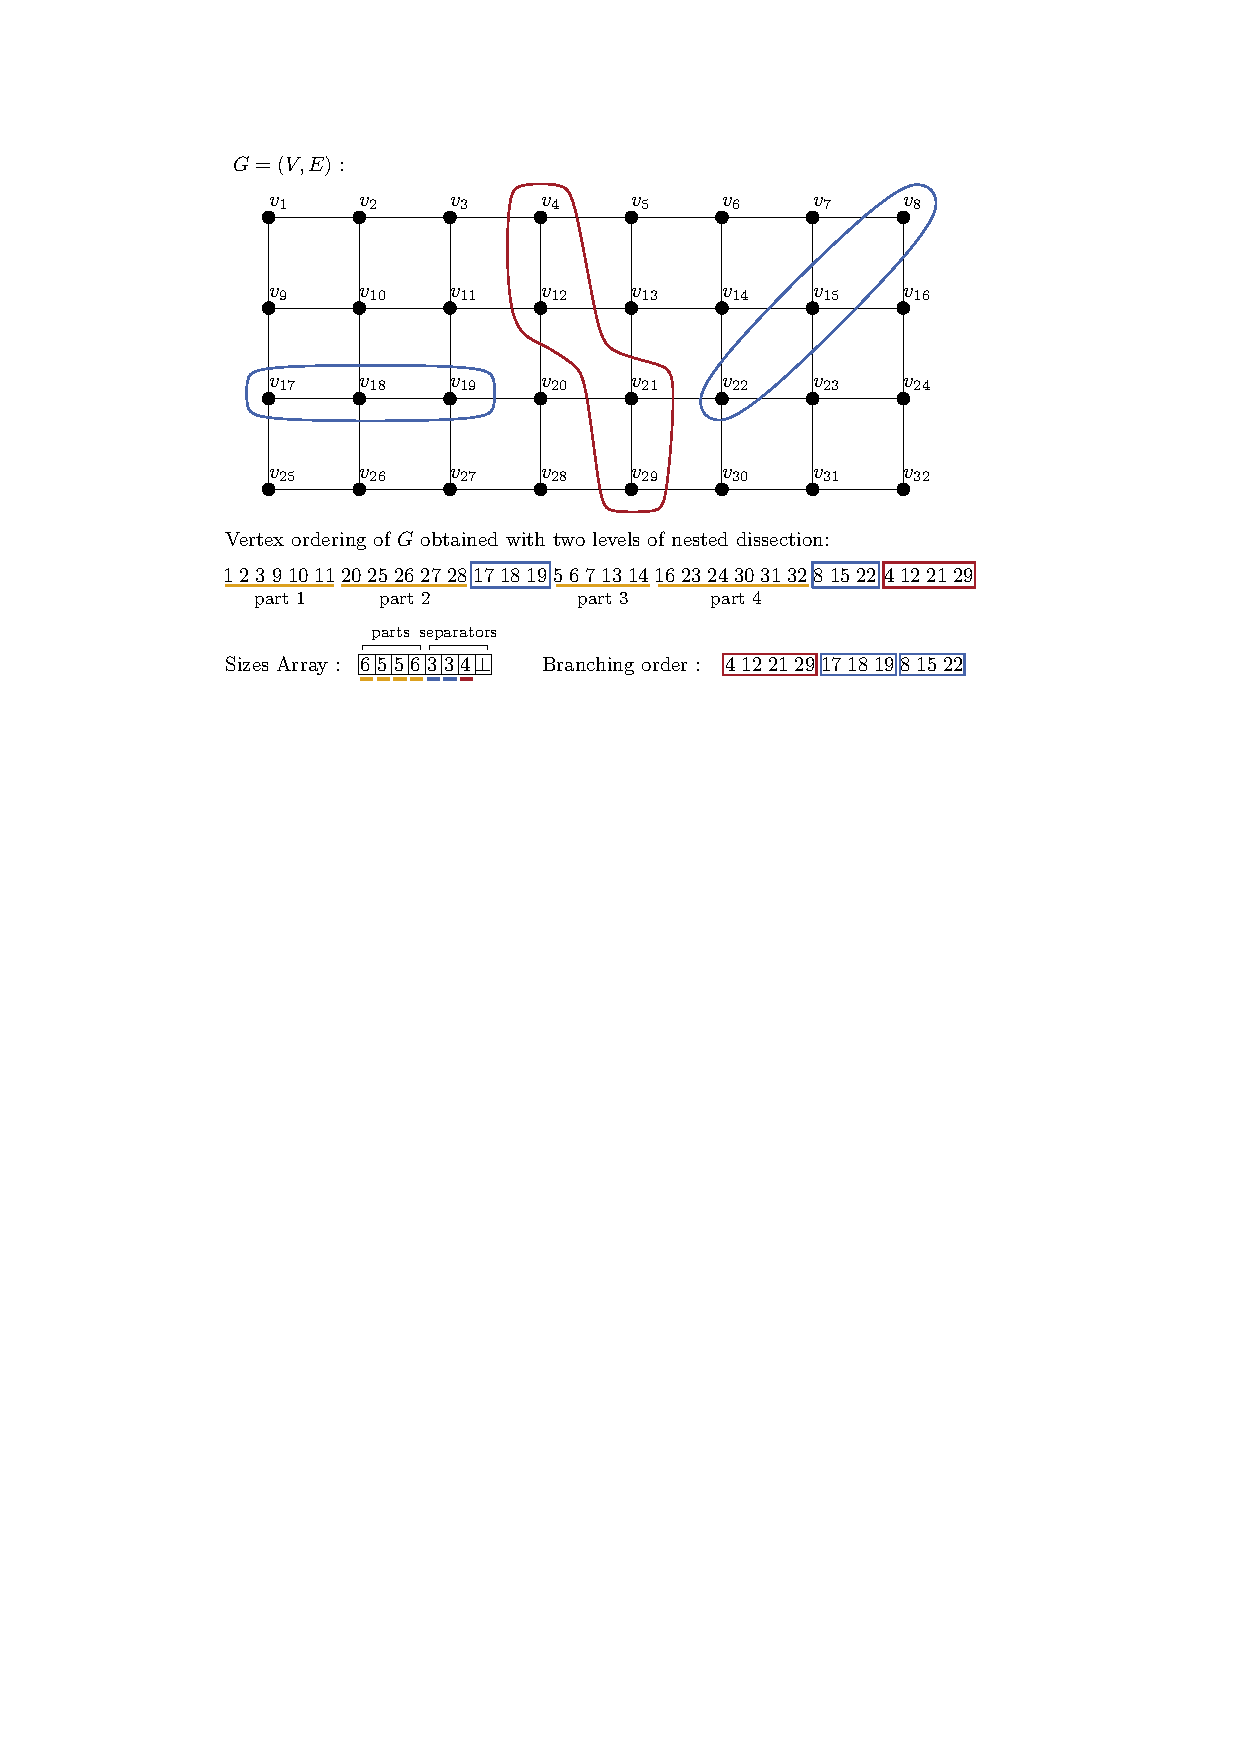
\includegraphics[scale=1.1]{images/restricted_nd}
	\centering
	\caption{Possible vertex ordering of the $8$ by $4$ grid obtained with two levels of nested dissection along with the sizes array and the extracted branching order}
	\label{fig:nd}
\end{figure}

\paragraph{}
In the implementation of our following branching strategy (Algorithm \ref{alg:nd}) a nested dissection ordering is computed immediately prior to the first branching step, i.e., after the initial kernelization step. To calculate the nested dissection ordering, we use an algorithm provided in the METIS library~\cite{METIS}. We do not apply a custom configuration to the algorithm, but rather use the default settings of the METIS library. Afterwards, the vertices are inserted into a queue in reverse nested dissection ordering. In each branching step, the branching strategy removes vertices from the queue until it finds a vertex that is still contained in the current graph. Finally, the respective vertex is returned for branching.

\begin{algorithm}
	\caption{NestedDissectionBranching}\label{alg:nd}
	\SetKwFunction{U}{NestedDissectionBranching}
	\SetKwFunction{A}{ExtractSeparators}	
	\SetKwFunction{D}{MaxDegBranching}
	\SetKwFunction{ND}{METIS\_NodeNDP}
	\DontPrintSemicolon
	\nonl\texttt{Global variables:} A vertex ordering $BO$ for branching, and a boolean $BOComputed$ which indicates whether an ordering has been computed\\
	\KwIn{A graph $G=(V,E)$ }
	
	\U{$G$}	
	\Begin{
		\If{$\lnot BOComputed$}{
			$(\sigma, sizes) \leftarrow $  \ND{$G$, $LevelsOfRecursions$}\tcp*{compute nested dissecton}
			\tcp*{ordering with respective sizes array}
			$BOComputed\leftarrow\texttt{true}$\\
			\For{$i\in\{2^{LevelsOfRecursions}+1,\dots,2^{LevelsOfRecursions+1}-1\}$}{\If{$sizes[i]>MaxSeparatorSize$}{$BOComputed\leftarrow\texttt{false}$\tcp*{separator is to large}\texttt{break} }}
			\If{$BOComputed$}{$BO\leftarrow$ \A{$\sigma$, $LevelsOfRecursions$, $sizes$}}
		}
		$v\leftarrow \bot$\\
		\eIf{$BOComputed$}{
			\For{$i\in\{1,\dots,|BO|\}$}{\If{$BO[i]\in V$}{\Return $BO[i]$\tcp*{find next vertex in the branching order}}}	
	}
		{$v\leftarrow\D{G}$\tcp*{use fallback}}
		\Return $v$
	}
	
	\KwOut{a branching order}
	
\end{algorithm}


\paragraph{} 
During initial tests of our implementation we noticed that branching on separators which come later in the reversed nested dissection ordering (i. e., separators obtained in a recursive call of higher depth), frequently does not result in decomposition of the graph. This is due to the fact that in addition to branching, the graph is also reduced by kernelization in each step of the algorithm. Thus, separators in the original graph are not necessarily separators in the current graph at the time of branching. Counteracting this, we optimized our branching strategy by performing a restricted number of levels of recursions instead of calculating a full nested dissection ordering. Then the branching order is composed solely by the separators obtained in those levels of recursion. In a branching step, if there are no more vertices left in the ordering, the default branching strategy is used as a fallback. The exact number of recursions used is a tuning parameter. Details are discussed in the following section (Section~\ref{sec5}).
\paragraph{}
To implement this optimization, we used an alternate method provided by the METIS library, which just performs a specified number of resursive calls of the nested dissection algorithm. Nevertheless, the problem remains that the algorithm still returns an ordering of all vertices of the graph. We are, however, only interested in the vertices contained in the separators of each recursive call. Luckily, the METIS library provides an array that stores the sizes of the parts as well as the separators for each level of recursion. The following recursive algorithm (Algorithm~\ref{alg:extract}) capitalizes on this feature by extracting the individual separators from the vertex ordering and constructing the branching ordering in the following manner.

\paragraph{}
The algorithm receives the vertex ordering and the sizes array as input. Initially, the branching order is empty. In each recursive call the algorithm starts by retrieving the size $k$ of the top level separator from the sizes array. Thereafter, the top level separator, which just contains the last $k$ vertices of the vertex ordering is inserted into the branching order. Then the algorithm splits the rest of the vertex ordering and the sizes array in accordance to the recursion. This results in orderings for each part of the bipartition and the two corresponding sizes arrays. Subsequently, the separators residing in those parts are extracted recursively and are added to the branching order.
\paragraph{}
As in the previous branching strategy using edge cuts, we optimize our implementation by considering a vertex ordering only if the sizes of the vertex separators computed at each level of recursion are not exceeding a certain threshold. The exact value of the threshold is a tuning parameter. In contrast to the previous branching strategy, we did not tweak the balancing constraints used by the nested dissection algorithm. 

\paragraph{}
Another optimization we tested was to compute a new nested dissection ordering (with restricted levels of recursion) following removal of all vertices of the previous ordering from the graph. This way, we attempt to combine the advantage of using a static branching ordering with choosing vertices dynamically on the current graph.  However, tests showed that this variant of the branching strategy performs worse than computing the vertex ordering only once. A possible explanation is that branches at a lower depth of recursion have a greater impact on the total number of branches needed than such at a higher depth. Hence, decomposing the graph at an early stage in the algorithm is more powerful than at later stages. An alternate reason might be that branches at a higher depth of recursion are more likely to be pruned before all vertices of a separator have been removed by branching. 

\subsection{Branching Strategies Based on Reduction Rules} \label{red_strats}

The branching strategies described in this section are essentially based on the break up of structures that can not be reduced by kernelization. The core idea behind this is to identify vertices such that branching on those enables the application of reduction rules afterwards. Our initial approaches using this concept are rather simple and attempt to find single vertices that prevent a certain reduction rule from being applicable. It is generally advantageous that finding of such vertices can be accomplished during kernelization without noticeable time overhead.
\paragraph{}
Following this idea, we implemented and tested four branching strategies each targeting a different reduction rule. Finding of potential candidates for branching, i.e., vertices that prevent the corresponding reduction rule from being applicable, works differently depending on the targeted reduction rule. However, the actual branching step is the same for all these variants (see Algorithm \ref{alg:red_branch}). In a branching step, a vertex for branching is chosen from a set of vertices managed by the respective branching strategies. Vertices considered for branching are inserted into this set during kernelization. Notice that at the time of branching, vertices in the set could have already been removed from the graph by another reduction rule. Thus, reduced vertices have to be filtered out first. Subsequently, if the set of branching vertices is not empty, all four branching strategies choose a vertex of highest degree from the set and return it for branching. Otherwise, if there are no vertices in the set, the default branching strategy is used as a fallback.

\paragraph{}
As in the case of the branching strategies described in Section \ref{decomp}, our implementations are optimized to the effect that even if the set of potential branching vertices is not empty, only vertices of a certain degree are considered for branching. Details on how the tuning parameter is chosen are explained in Section \ref{sec5}.

\begin{algorithm}
	\caption{ReductionBranching}\label{alg:red_branch}
	\SetKwFunction{U}{ModifiedTwinReduction}
	\SetKwFunction{A}{ApplyTwinReduction}	
	\SetKwFunction{D}{MaxDegBranching}
	\DontPrintSemicolon
	\nonl\texttt{Global variables:} A set $BV$ of vertices considered for branching\\
	\KwIn{A graph $G=(V,E)$ }
	
	\U{$G$}	
	\Begin{
		$v\leftarrow \bot$ ; 
		$dv\leftarrow -1$\\
		\For{$u\in BV$}{
			\If{$d(u) > d(v)$}{
				$v \leftarrow u$ \tcp*{find vertex with maximum degree of all vertices considered}
				$dv \leftarrow d(u)$
			}
		}
		\If{$v = \bot \lor dv < \Delta(G) - DegThreshold$}{$v\leftarrow$ \D{$G$}\tcp*{use fallback}}
		\Return $v$
		
	}
	
	\KwOut{a vertex $v$ for branching}
	
\end{algorithm}

\paragraph{}
In the following, we describe for each of the four branching strategies how vertices considered for branching are found during kernelization.

\subsubsection{Branching Based on Twin Reduction}
The first branching strategy in this subsection is based on the Twin reduction rule (covered in Section~\ref{red}). To characterize the structure in which a single vertex prevents the twin reduction from being applicable, consider the following definition.

\begin{definition} (Almost Twins)
	In a graph $G=(V,E)$ two non adjacent vertices $u$ and $v$ are called almost twins if $d(u) = 4$, $d(v) = 3$ and $N(v)\subseteq N(u)$ (i.e. $N(u) = N(v) \cup \{w\}$). 
\end{definition}

Clearly, after removing $w$, it holds that $d(u)=d(v)=3$ and $N(u)=N(v)$. Thus, by removing $w$, the vertices $u$ and $v$ become twins. Consequently, the twin reduction rule is applicable afterwards. Thus, when using this branching strategy, the branch and reduce algorithm searches for pairs of vertices that are almost twins during each kernelization step. Finding those vertices can be done while already searching for twins. The twin reduction rule checks for each vertex $v$ of degree three if there is a vertex $u \in N^2(v)$ such that $d(u) = 3$ and $N(u)=N(v)$. To find almost twins, we modify this routine (Algorithm \ref{alg:alm_twins}) in order to simultaneously check if there is a vertex $u \in N^2(v)$ with $d(u) = 4$ and $N(v)\subseteq  N(u)$. If such a pair of vertices $u$ and $v$ is found, the single vertex $w\in (N(u)\cup N(v))\setminus(N(u) \cap N(v))$ is inserted into the set of vertices considered for branching. An example for almost twins is depicted in Figure \ref{fig:alm_twin}.\\

\begin{figure}[htb]
	\captionsetup{belowskip=1em}
	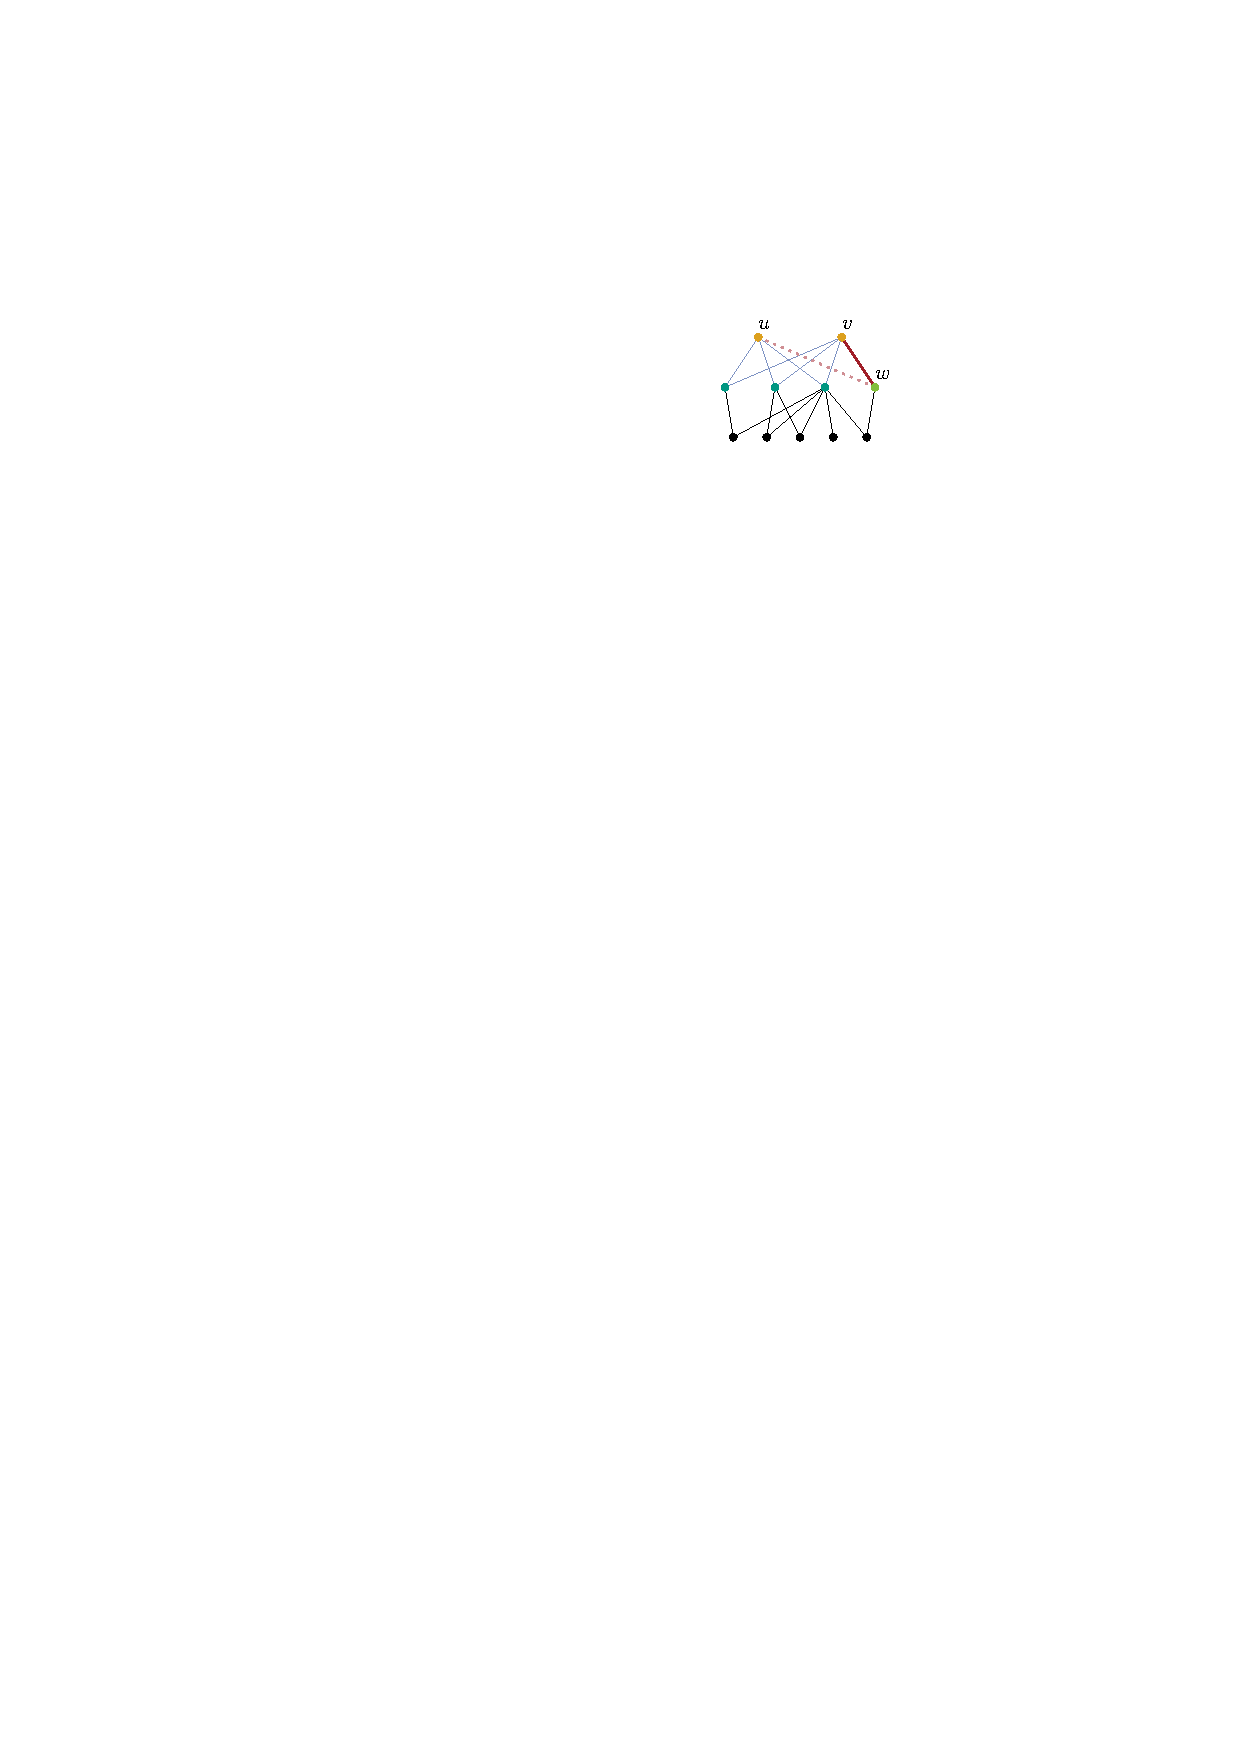
\includegraphics[scale=1.5]{images/alm_twin}
	\centering
	\caption{The vertices $u$ and $v$ are almost twins. Upon removal of vertex $w$, $u$ and $w$ become twins and, consequently, twin reduction can be applied.}
	\label{fig:alm_twin}
\end{figure}

\begin{algorithm}[htb]
	\caption{ModifiedTwinReduction}\label{alg:alm_twins}
	\SetKwFunction{U}{ModifiedTwinReduction}
	\SetKwFunction{A}{ApplyTwinReduction}
	\DontPrintSemicolon
	\nonl\texttt{Global variables:} A set $BV$ of vertices considered for branching\\
	\KwIn{A graph $G=(V,E)$ }
	
	\U{$G$}	
	\Begin{
		$BV \leftarrow \emptyset$\tcp*{Vertices considered for branching}
		\ForEach{$v\in V$}{
			\If{$d(v)=3$}{
				\ForEach{$u\in N^2(v)$}{
					\If{$d(u) = 3 \land N(u)=N(v)$}{\A{$v$, $u$} \tcp*{$v$ and $u$ are twins; apply reduction}}	
					\ElseIf{$d(u) = 4 \land N(v)\subseteq N(u)$}{$BV\leftarrow BV\cup(N(u)\setminus N(v))$\tcp*{$v$ and $u$ are almost twins}}
				}
			}
		}
		\Return $BV$
	}
	
	\KwOut{a set of verices considered for branching}
	
\end{algorithm}

\subsubsection{Branching Based on Funnel Reduction}
For the second branching strategy we attempt to find vertices preventing application of the alternative reduction. As mentioned in Section~\ref{red}, the branch and reduce algorithm only utilizes the special cases funnel and desk reduction, hence providing a further restriction in regards to eligible reduction rules. However, desk reduction is based on a very concrete graph structure and therefore is rarely applied in our benchmark instances; in contrast, funnel reduction is applied more often. Also, it is difficult to determine if a vertex prevents the desk reduction from being applicable, since a multitude of cases would have to be considered.
For those reasons, we do not target the desk reduction, but exploit the funnel reduction rule instead.
\paragraph{}
Similar to the first branching strategy, we define the structure within which the funnel reduction can be applied upon removing a single vertex.
\begin{definition}(Almost Funnel)
	In a graph $G=(V,E)$ two adjacent vertices $u$ and $v$ are called almost funnels if $u$ and $v$ are not funnels and there is a vertex $w$ such that $N(v)\setminus\{u,w\}$ induces a clique.
\end{definition}

By removing the single vertex $w$, $u$ and $v$ become funnels and, thus, $u$ can be reduced afterwards. Pairs of vertices that are almost funnels can be found easily during the funnel reduction. To check whether two vertices $u$ and $v$ are funnels, the funnel reduction rule iterates over the vertices in $N(v)\setminus \{u\}$ and checks, if they are adjacent to the previous vertices in the iteration. Once it finds a vertex that is not adjacent to all prior vertices, the reduction rule concludes that $u$ and $v$ are not funnels and stops checking the remaining neighbors of $v$. To find almost funnels we modify this procedure as follows (Algorithm \ref{alg:alm_funnels}). We still iterate over $N(v)\setminus\{u\}$ and check for adjacency. Once a vertex $w$ is found that is not adjacent to all prior vertices, two cases are considered. Firstly, if $w$ is not adjacent to at least two preceding vertices, then $u$ and $v$ representing almost funnels can be verified by checking if $N(v)\setminus\{u,w\}$ induces a clique. In the second case there is only one vertex $w'$ prior to $w$ such that $w'$ and $w$ are not neighbors. Then $u$ and $v$ are almost funnels, if $N(v)\setminus\{u,w\}$ or $N(v)\setminus\{u,w'\}$ induces a clique. In both cases, if $u$ and $v$ are almost funnels, the neighbor of $v$, which is not contained in the induced clique (i.e. $w$~or~$w'$ respectively), is inserted into the set of vertices considered for branching. A structure with almost funnels is shown as an example in Figure \ref{fig:alm_funnel}.

\begin{figure}[htb]
	\captionsetup{belowskip=-1em}
	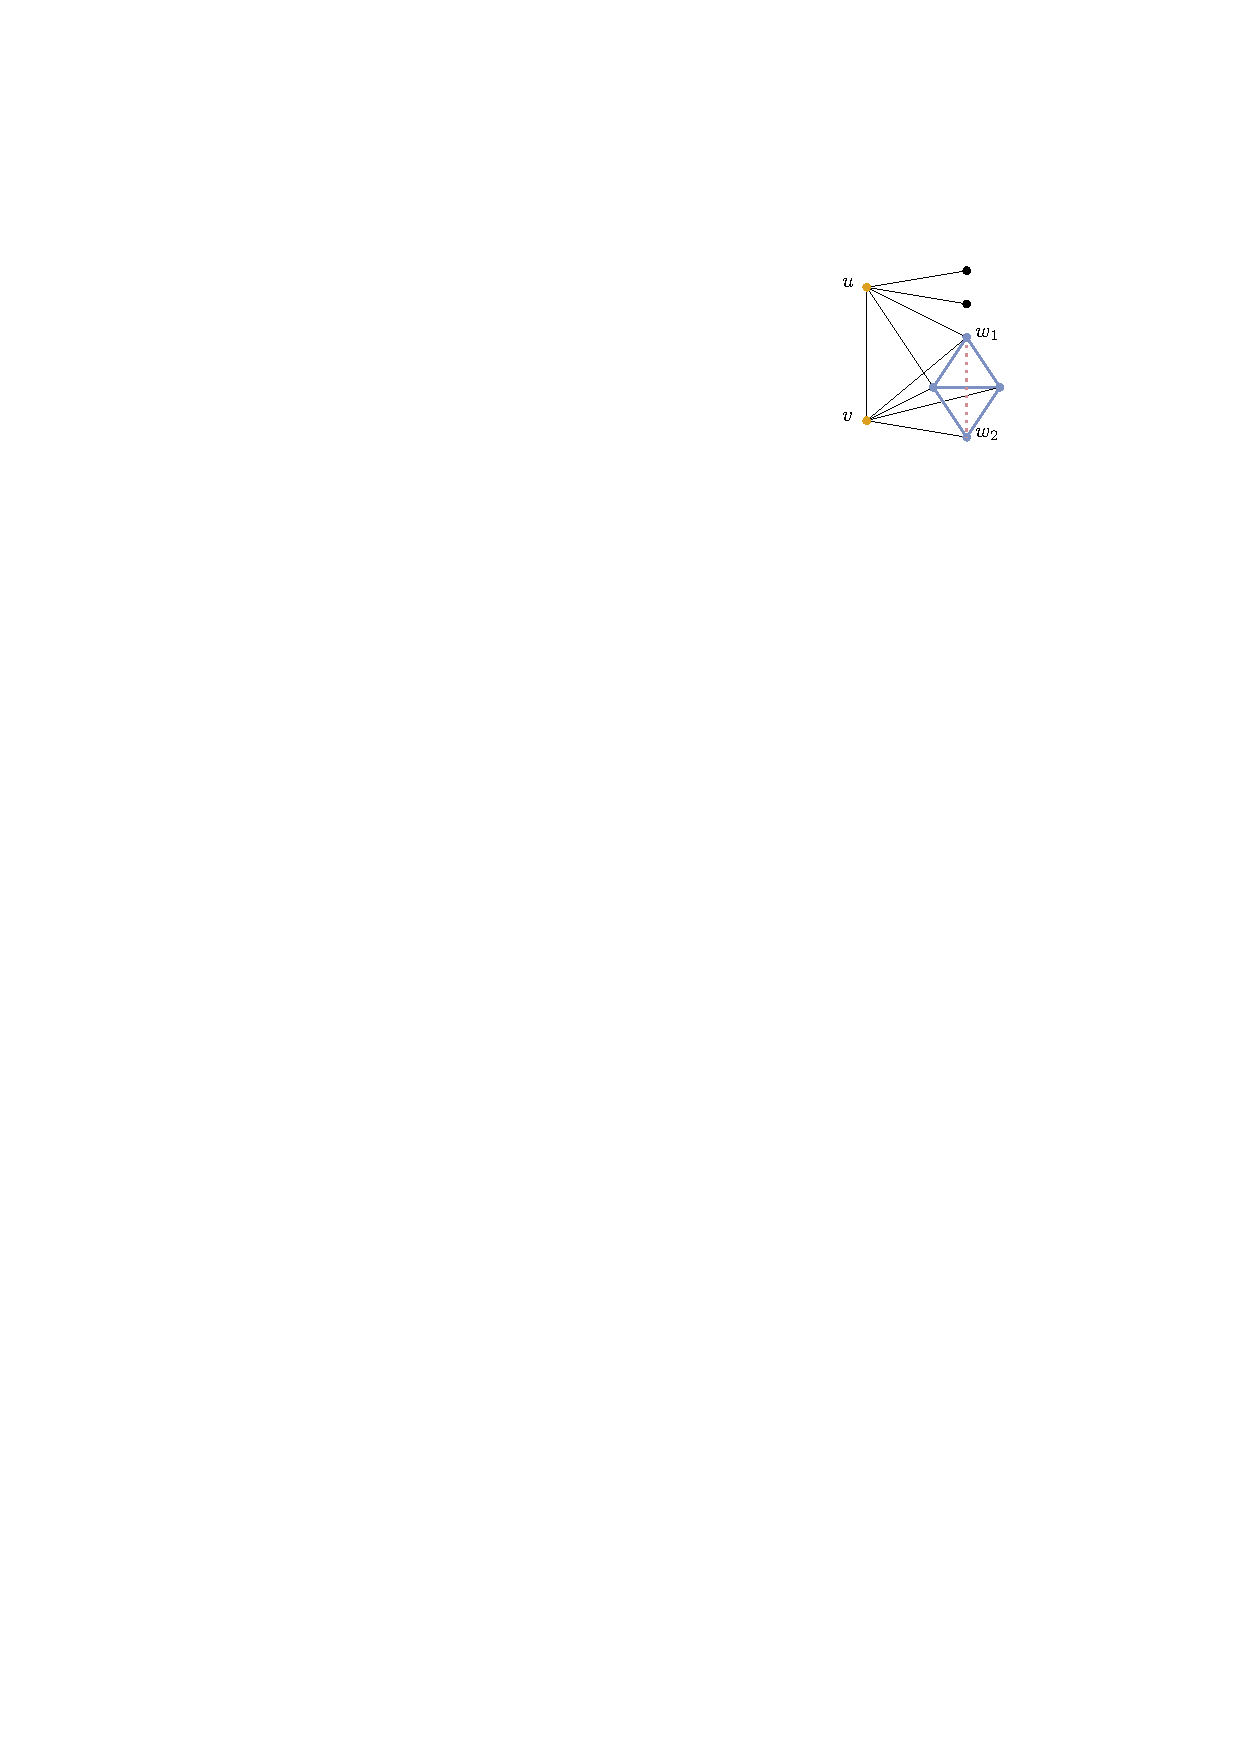
\includegraphics[scale=1.5]{images/alm_funnel}
	\centering
	\caption{The vertices $u$ and $v$ are almost funnels. $N(v)\setminus\{u\}$ is highlighted in blue. After removing either $w_1$ or $w_2$, $N(v)\setminus\{u\}$ induces a clique. Thus, $u$ and $v$ become funnels and consequently, funnel reduction can be applied.}
	\label{fig:alm_funnel}
\end{figure}

\begin{algorithm}[htb]
	\caption{CheckAlmostFunnel}\label{alg:alm_funnels}
	\SetKwFunction{U}{CheckAlmostFunnel}
	\SetKwFunction{A}{ApplyFunnelReduction}
	\DontPrintSemicolon
	\nonl\texttt{Global variables:} A set $BV$ of vertices considered for branching\\
	\KwIn{A graph $G=(V,E)$, vertice $v$ and $u$ }
	
	\U{$G$, $v$, $u$}	
	\Begin{
		$x \leftarrow \bot$ ;  $y \leftarrow \bot$ ; $C\leftarrow \emptyset$
		\ForEach{$w\in N(v)\setminus\{u\}$}{
			\eIf{$C\subseteq N(w)$}{$C\leftarrow C\cup\{w\}$}{
				\eIf{$|C\setminus N(w)| > 1$}{
					\If{$x\neq \bot$}{\Return\tcp*{$v$ and $u$ are neither funnels nor almost funnels}}
					$x\leftarrow w$}
				{\If{$x\neq \bot$}{\Return\tcp*{$v$ and $u$ are neither funnels nor almost funnels}}
					$x\leftarrow w$\\
					$y\leftarrow z \in C\setminus N(w) = \{z\}$\\
					$C \leftarrow C \setminus \{y\}$
				}
			}
		}
		\If{$x = \bot \land y = \bot $}{\A{$v$, $u$} \tcp*{$v$ and $u$ are funnels; apply reduction}}
		\ElseIf{$y = \bot$}{$BV \leftarrow BV \cup \{x\}$ \tcp*{$v$ and $u$ are almost funnels; consider $x$ for branching}}
		\Else {
			\If{$C\subseteq N(x) $}{$BV \leftarrow BV \cup \{y\}$\tcp*{$v$ and $u$ are almost funnels; consider $y$ for branching}}	
			\ElseIf{$C\subseteq N(y) $}{$BV \leftarrow BV \cup \{x\}$\tcp*{$v$ and $u$ are almost funnels; consider $x$ for branching}}	
	}
		\Return $BV$
	}	
	
\end{algorithm}

\subsubsection{Branching Based on Dominance Reduction}
The third branching strategy is making use of the dominance reduction rule. Again, we define the structure which contains a vertex enabling dominance reduction upon removal.

\begin{definition} (Almost Dominance)
	In a graph $G=(V,E)$ a vertex $u$ is called almost dominated by a neighbor $v$ if $|N(u)\setminus N(v)| = 1$ and $N[v]\not\subseteq N(u)$.
\end{definition}

The condition $N[v]\not\subseteq N(u)$ ensures that $v$ is not already dominated by $u$. By removing the single vertex $w\in N(u)\setminus N(v)$, the vertex $u$ becomes dominated by $v$, since $(N[u]\setminus\{w\})\subseteq N(v)$. Similar to the previous branching strategy, we search for pairs of vertices $u$ and $v$ such that $u$ is almost dominated by $v$. The dominance reduction verifies whether a vertex $u$ is dominated by $v$ through checking if all neighbors of $u$ are also neighbors of $v$. Once it finds a vertex that is adjacent to $u$ but not a neighbor of $v$, it is concluded that $u$ is not dominated by $v$ and the remaining vertices are not going to be checked anymore. We modify the dominance reduction to test if the neighbors of $u$ are adjacent to $v$ until either all neighbors have been checked or, alternatively, a second vertex adjacent to $u$ is found that is not also a neighbor of $v$. When all vertices have been checked and there is no vertex $w \in N(u)\setminus N(v)$, then $u$ is dominated by $v$. Otherwise, $w$ is inserted into the set of vertices considered for branching. An example for almost dominance is illustrated in Figure \ref{fig:alm_dom}.\\

\begin{figure}[htb]
	\captionsetup{belowskip=-1em}
	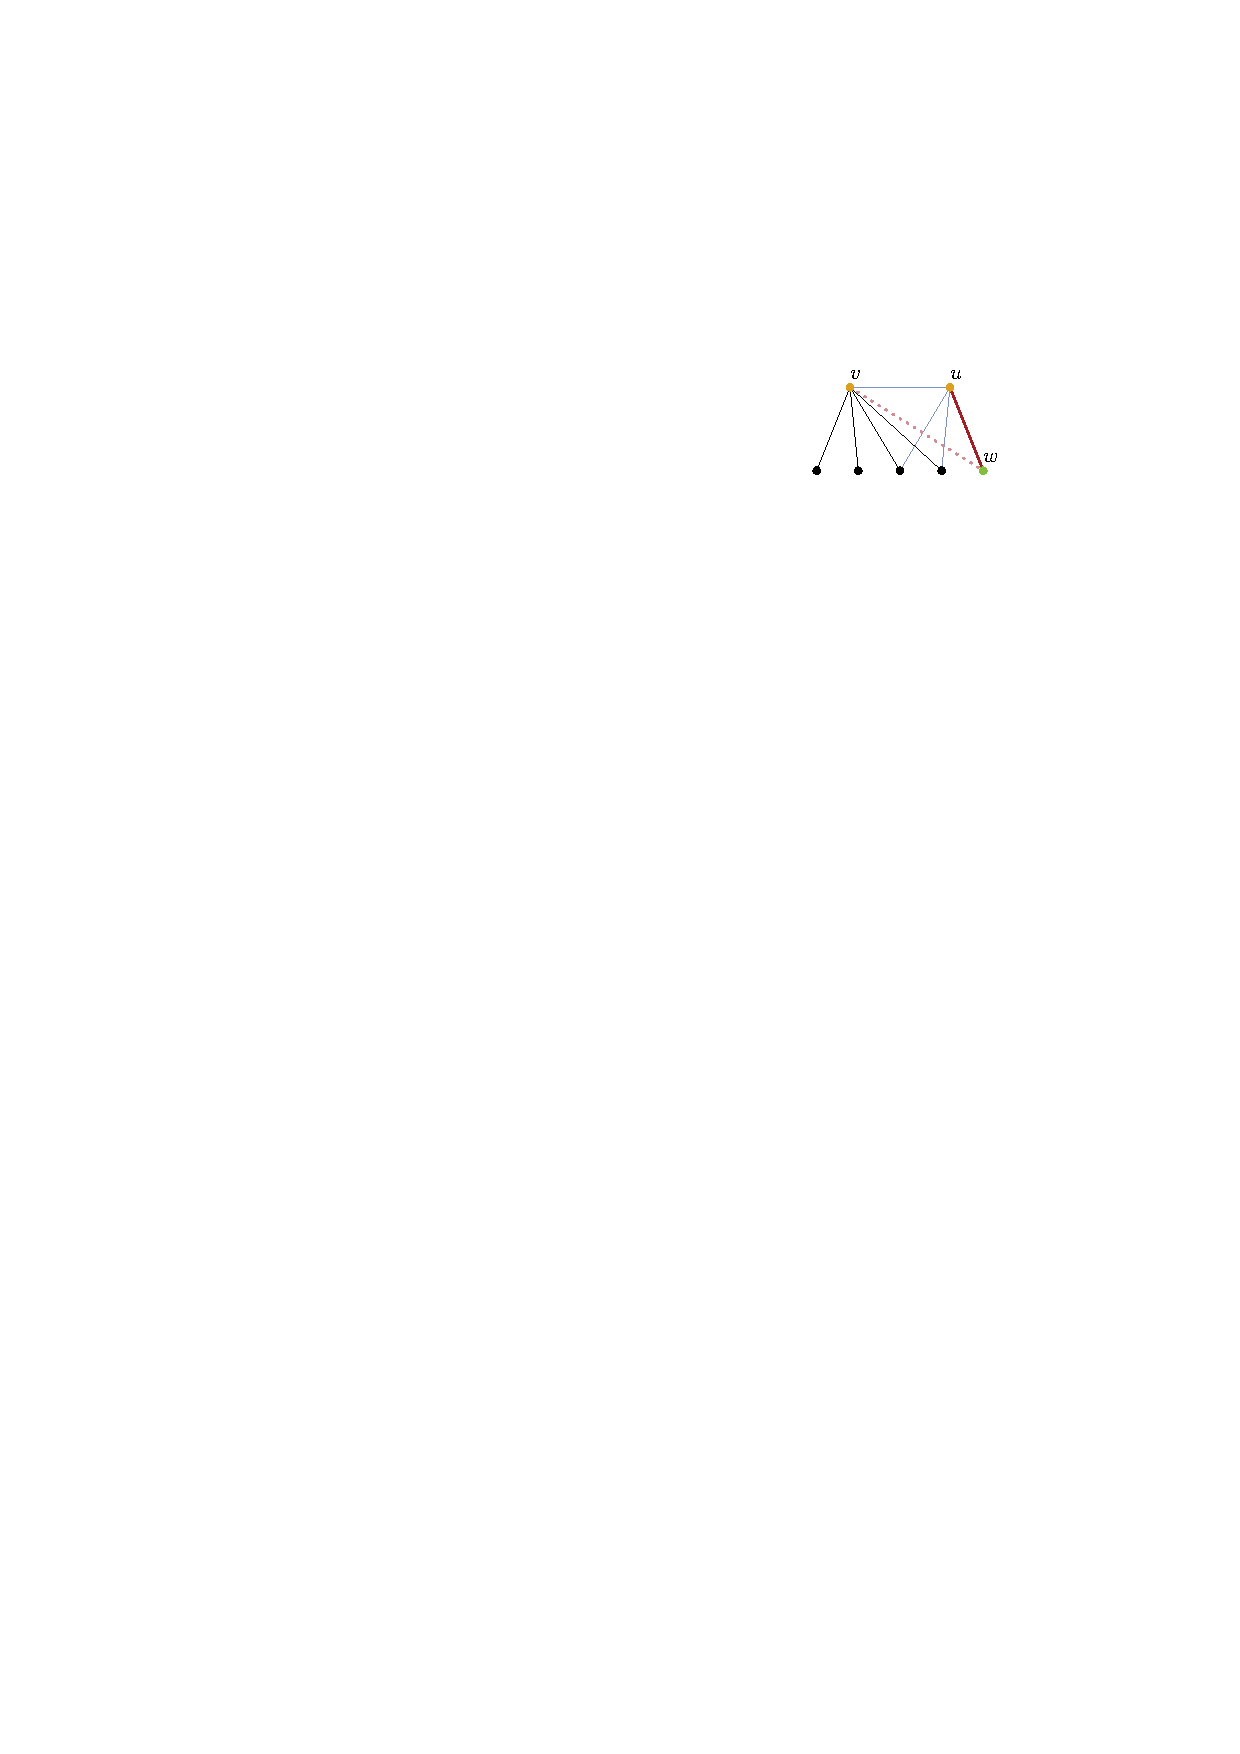
\includegraphics[scale=1.5]{images/alm_dom}
	\centering
	\caption{The vertex $u$ is almost dominated by $v$. After removing $w$, $u$ is dominated by $v$ and thus, $v$ can be removed by dominance reduction.}
	\label{fig:alm_dom}
\end{figure}

\begin{algorithm}
	\caption{CheckAlmostDominance}\label{alg:alm_dominance}
	\SetKwFunction{U}{ModifiedDominanceReduction}
	\SetKwFunction{A}{ApplyDominanceReduction}
	\DontPrintSemicolon
	\nonl\texttt{Global variables:} A set $BV$ of vertices considered for branching\\
	\KwIn{A graph $G=(V,E)$, vertices $v$ and $u$}
	
	\U{$G$, $v$, $u$}	
	\Begin{
		$x \leftarrow \bot$ \\
		
				\ForEach{$w\in N(u)\setminus\{v\}$}{
					\If{$w\notin N(v)$}{
						\eIf{$x = \bot$}{$x = w$}{\Return\tcp*{$u$ is neither dominated nor almost dominated by $v$}}}
					}
				
			\eIf{$x = \bot$}{\A{$v$, $u$}\tcp*{$u$ is dominated by $v$; apply reduction}}{$BV \leftarrow BV \cup \{x\}$\tcp*{$u$ is almost dominated by $v$; consider $x$ for branching}}
	}
	
	
\end{algorithm}

\paragraph{}
A fundamental difference to the two preceding branching strategies is that the dominance reduction rule is not actually used by the branch and reduce algorithm. Nevertheless, dominance reduction is fully contained in the unconfined reduction rule used by the algorithm so that dominating vertices still get reduced. It is a major drawback, however, that vertices considered for branching making the dominance rule become applicable, can not be found during kernelization. Instead, one has to search for such vertices separately after kernelization resulting in a non-negligible time overhead. 

\subsubsection{Branching Based on Unconfined Reduction}
Therefore, in the fourth branching strategy we generalize the previous strategy in order to exploit the unconfined reduction rule. We define an almost unconfined vertex analogously to the previous definitions.

\begin{definition} (Almost Unconfined)
	In a graph $G=(V,E)$ a vertex $v$ is called almost unconfined if $v$ is not unconfined but there is a vertex $u$ such that $v$ is unconfined in $G-u$.
\end{definition}

By definition, $v$ becomes unconfined after removing $u$ and, thus, by means of the unconfined reduction rule can also be removed. However, it is not clear how to determine whether a vertex $u$ is almost unconfined and, moreover, how to find the specific vertex $u$ preventing $v$ from being unconfined. There are basically two cases to be considered. Firstly, at some point during the execution of the unconfined algorithm (Algorithm \ref{alg:unconf}) there is an extending child, i. e., a child $w$ with $\{u\} = N(w) \setminus N[S]$, and, coincidentally, inclusion of $u$ into the set $S$ leads to $v$ not being unconfined. By removing $u$, vertex $w$ becomes a child devoid of neighbors not being already contained in $N[S]$. Thus, $v$ becomes unconfined. In the second case, at the end of the unconfined algorithm there is a child $w$ with $\{u,x\} = N(w) \setminus N[S]$. Upon removing $u$, the vertex $w$ becomes an extending child. Therefore, the unconfined algorithm has to include $x$ into the set $S$ and eventually concludes that $v$ is unconfined. 

It is easy to check whether the first case occurs, assuming there is only one extending child at some point during the algorithm. In each step of the modified unconfined algorithm (see Algorithm \ref{alg:mod_unconf}), if there is only one extending child $w$ with $\{u\} = N(w) \setminus N[S]$, we insert $u$ into a buffer. When the algorithm terminates, the following condition applies. If it returns false and the buffer is not empty, then $v$ is almost unconfined and removal of any vertex from the buffer makes $v$ unconfined. Hence, all vertices from the buffer can be considered for branching. Unfortunately, this approach does not work, if there are more than one extending child in every step of the unconfined algorithm.

Notably, there is also an obstacle in detecting the second case. If the unconfined algorithm concludes a vertex $v$ is not unconfined, we can in fact check if at the end of the unconfined algorithm there is a child $w$ with $\{u,x\} = N(w) \setminus N[S]$; but we do not know if removal of either $u$ or $x$ is going to result in $v$ becoming unconfined. Hence, in this case we can not easily check whether $v$ is almost unconfined or not.

\begin{figure}[htb]
	\centering
	\captionsetup[subfigure]{aboveskip=1em,belowskip=1em}
	\captionsetup{belowskip=-1em, aboveskip=0em}
	\begin{subfigure}{\textwidth}
		\centering
		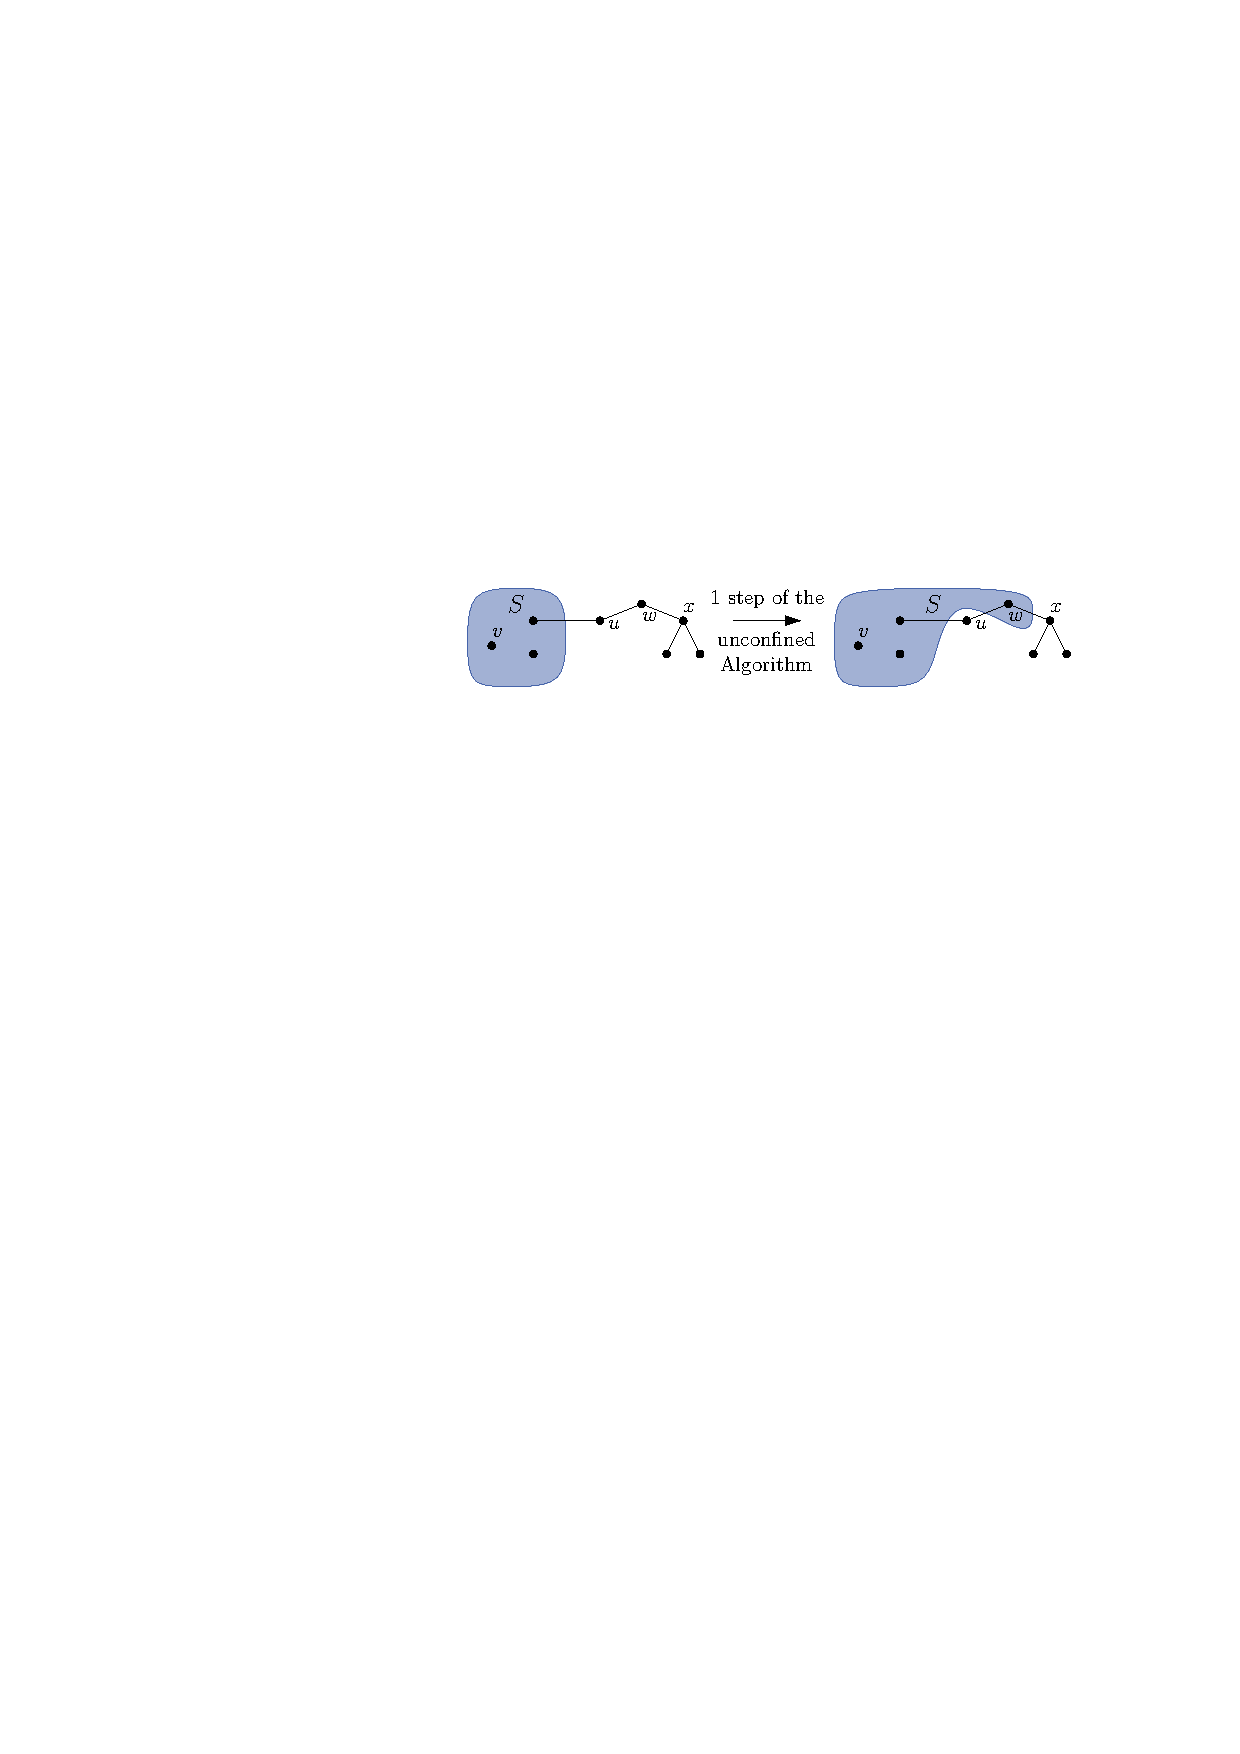
\includegraphics[scale=1.5]{images/alm_unconf_1}
		\caption{Case one: the vertex $u$ is an extending child and thus, $w$ is included into the set $S$. Subsequently $x$ is the only child of $S$. However, $|N(x)\setminus N[S]| = 2$ and therefore $v$ is not unconfined. By removing $w$, $u$ becomes a child with $|N(u)\setminus N[S]| = 0$ and thus, $v$ is unconfined.  }
	\end{subfigure}
	\begin{subfigure}{\textwidth}
		\centering
		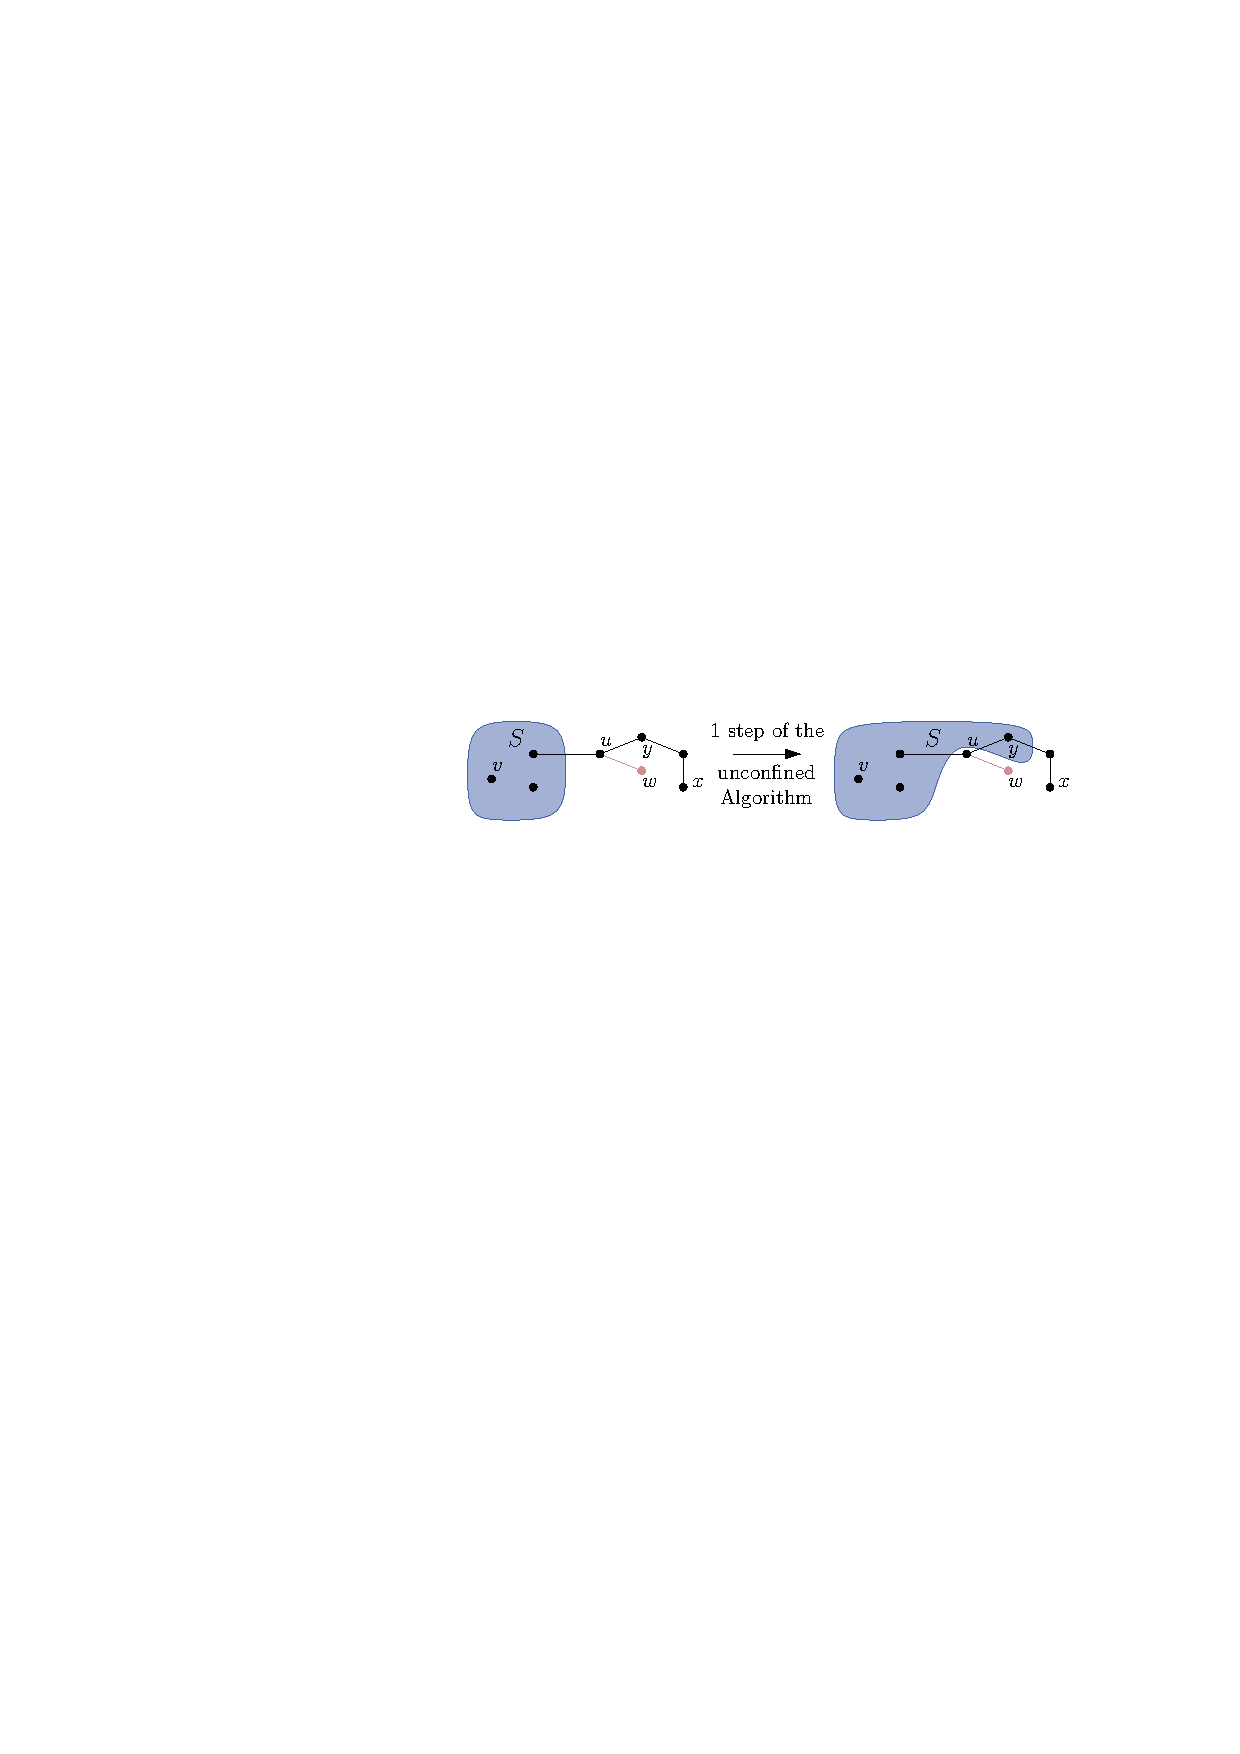
\includegraphics[scale=1.5]{images/alm_unconf_2}
		\caption{Case two: the vertex $u$ is the only child of $S$ with $|N(u) \setminus N(S)| = 2$. Thus, $v$ is not unconfined. By removing $w$, the vertex $u$ becomes an extending child and $y$ is included into $S$. Subsequently, $x$ becomes a child with $|N(x)\setminus N[S]| = 0$ and $v$ is unconfined.}
	\end{subfigure}
	\caption{The vertex $v$ is almost unconfined.}
\end{figure}

\begin{algorithm}
	\caption{ModifiedUnconfinedReduction}\label{alg:mod_unconf}
	\SetKwFunction{U}{ModifiedUnconfinedReduction}
	\DontPrintSemicolon       
	  
	  
	\nonl\texttt{Global variables:} A set $BV$ of vertices considered for branching\\
	\KwIn{A graph $G$, a vertex $v$}
	\U{G, v}	
	\Begin{
		$B \leftarrow \emptyset$ \\
		$S \leftarrow \{v\}$\;
		\While{$S\text{ has child }u\text{ with } |N(u)\setminus N[S]|\leq 1$}{
			\eIf{$|N(u)\setminus N[S]| = 0$}{\Return true\tcp*{Contradiction to Theorem \ref{unconfined}}}{
				\If{$u$ is the only child with $|N(u)\setminus N[S] = 1$}{$B \leftarrow B  \cup \{w\}$}
				$\{w\}\leftarrow N(u)\setminus N[v]$\tcp*{By assumption $w$ also has to}
				$S\leftarrow S\cup\{w\}$\tcp*{be contained in every MIS}
			}
		}
		$BV \leftarrow BV\cup B$ \tcp*{if $B \neq \emptyset$, $v$ is almost unconfined; consider vertices in $B$ for branching}
		\Return $\text{false}$
		
	}
	
	\KwOut{true if $v$ is unconfined, false otherwise}
	
\end{algorithm}
\paragraph{}
Thus, during kernelization almost unconfined vertices can only be identified, if case one applies. Unfortunately, it is not clear whether this is true if a vertex $u$ is almost dominated by another vertex $v$. It holds that $v$ is either unconfined (then $v$ is reduced anyway) or, alternatively, $v$ is almost unconfined, since by removing the single vertex $w \in N(u)\setminus N(v)$, $u$ becomes dominated by $v$; hence, $v$ becomes unconfined. Also, during the unconfined procedure, $u$ is an extending child as long as the set $S$ does not contain $w\in N(u)\setminus N(v)$ following from $N(u)\setminus\{w\}\subseteq N(v)$. Hence, if $u$ is the only extending child at any point during the unconfined algorithm, then case one applies. However, there can also be another extending child being considered prior to $u$ by the unconfined algorithm, consequently forcing $w$ into the set $S$. In this instance, $u$ is no longer a child of $S$ and, eventually, case two might prevail. 
Moreover, if a vertex $v$ is almost unconfined, there can also be a vertex such that removing the latter results in $v$ being neither unconfined nor almost unconfined anymore. Notably, this vertex can also be removed during a branching step by the mirror branching rule (covered in Section \ref{red}).

\subsubsection{Branching on Reduction Chains}
During initial test runs using the first four branching strategies covered in this section, we observed that branching on a vertex may result in a whole series of reductions. There are two main causes for this. First, within one branching step multiple vertices frequently get removed from the graph. Specifically, this is the case when the branching vertex is included into the current solution and therefore its neighbors are excluded or, alternatively, when the branching vertex has mirrors (see Mirror branching rule in Section \ref{red}). Then, each of the removed vertices might enable a reduction during the following kernelization. The second cause is that removal of a vertex during branching might lead to a reduction which, in turn, enables further reductions. 
\paragraph{}
We make use of this observation in our fifth branching strategy. Here, the main idea is to choose a vertex with the effect that branching on this vertex is going to trigger a largest possible chain of reductions. Consider the following example shown in Figure \ref{fig:chain_red}. By removing the vertex $w$, $v$ becomes dominated by $u$, and therefore $u$ can be removed by dominance reduction. Subsequently, $x$ and $y$ become twins, and, finally, twin reduction can be applied.

\begin{figure}[htb]
	\captionsetup{belowskip=-1em}
	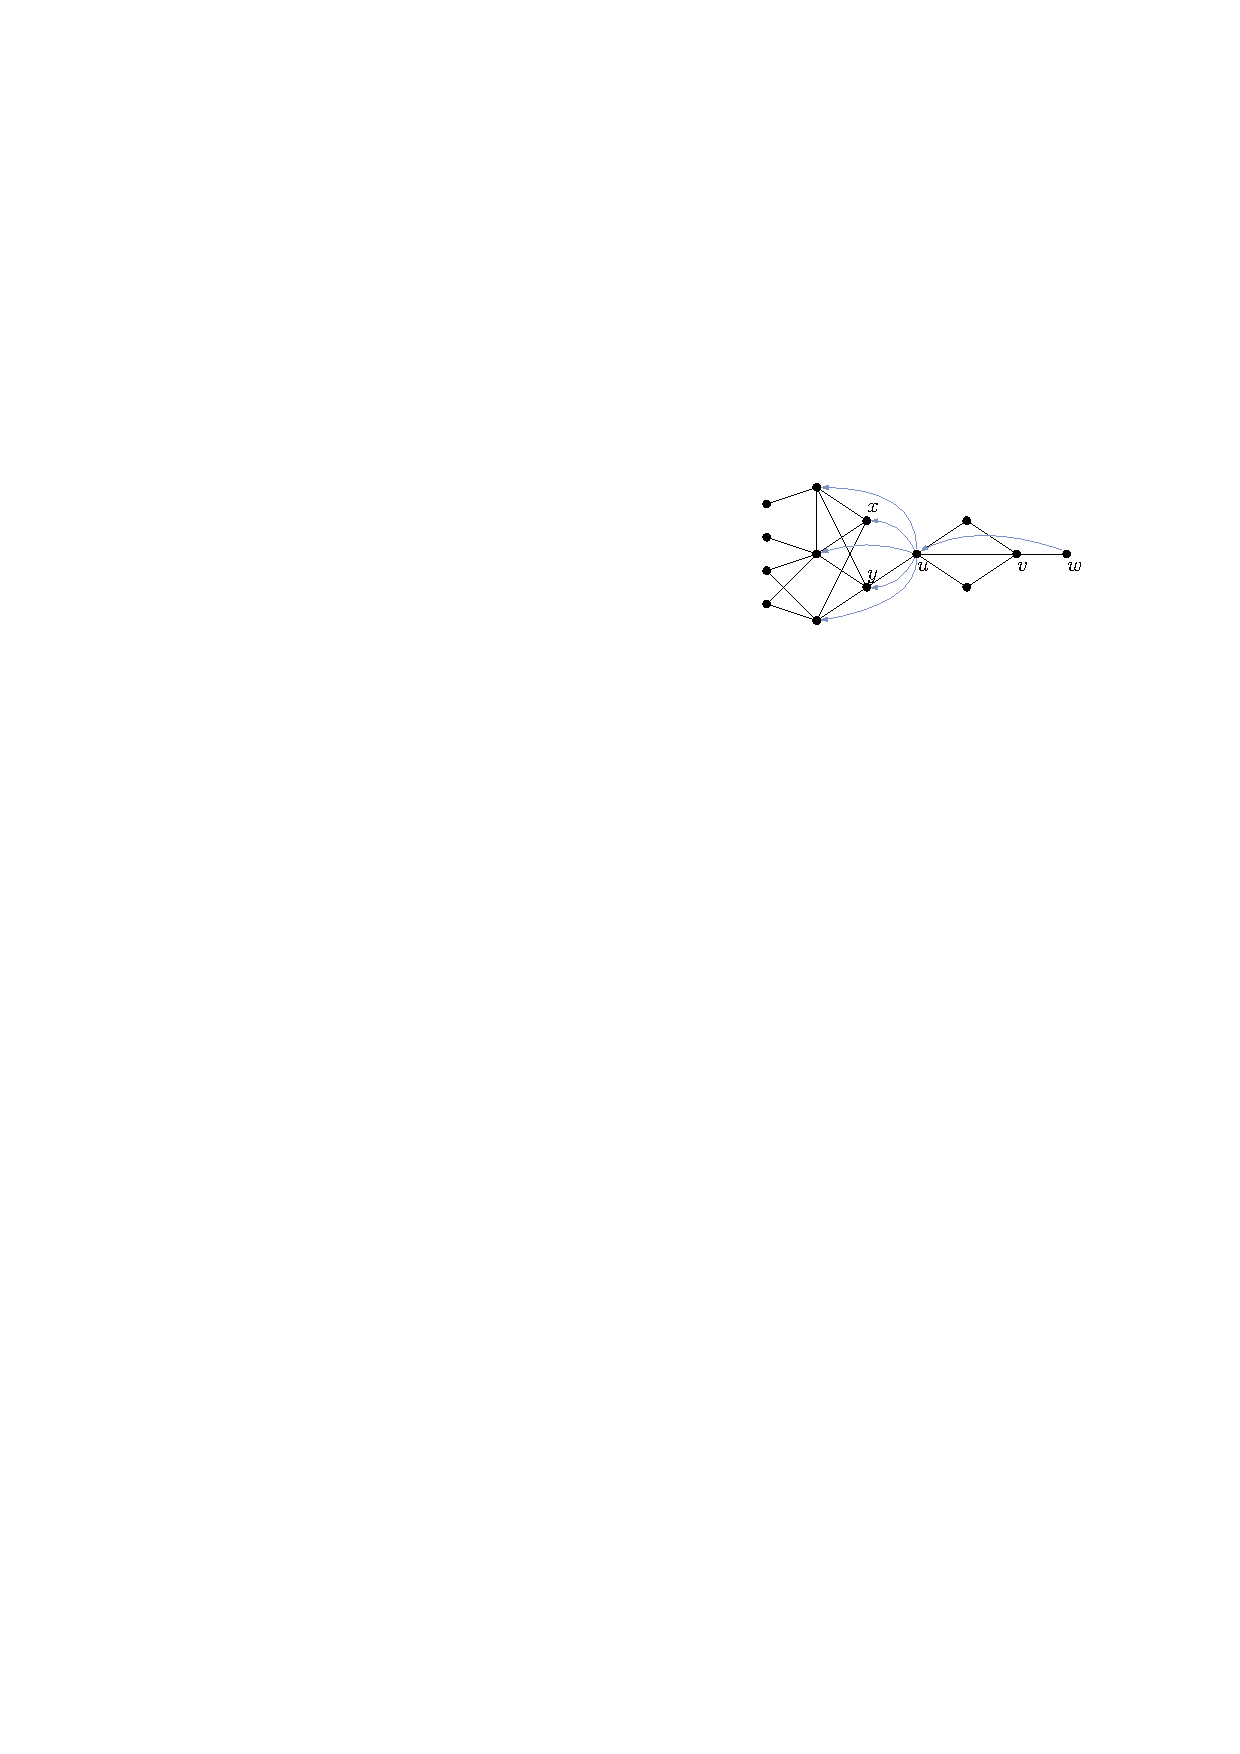
\includegraphics[scale=1.5]{images/chain_red}
	\centering
	\caption{Example for a reduction chain highlighted in blue}
	\label{fig:chain_red}
\end{figure}

\paragraph{}
To find large reduction chains we define the following directed graph $R=(V, E^\prime)$ where $V$ is just the vertex set of the original graph; further there is an edge from a vertex $u$ to another vertex $v$, if the removal of $u$ causes the reduction of $v$ based on a single reduction rule (we omit transitive edges). We call this a reduction graph. Given the reduction graph $R$, the number of vertices which can be reduced after removing a vertex $v$ at best corresponds to the number of vertices reachable from $v$ in $R$. We can compute this number with a simple BFS run starting at $v$.

\paragraph{}
Unfortunately, in practice the exact reduction graph is hard to construct as there are a few pitfalls. We can in fact use the results of our previous branching strategies to identify vertices that enable the reduction of other vertices upon their removal so that parts of the reduction graph can be constructed. However, in doing so, we do not consider all reduction rules used by the branch and reduce algorithm. Folding reductions, e.g., degree two folding or twin reduction add new vertices while alternative reductions introduce new edges between existing vertices. Consequently, those reductions might prevent other reductions. Also, we disregard the order in which the reduction rules are applied. Since the reduction rules are not executed iteratively but rather in a fixed order, it is therefore not guaranteed that the whole chain of reductions is performed in the right order. Moreover, the kernel sizes can be affected by the order in which reduction rules are applied. Thus, the number of vertices reachable in the reduction graph starting at a specific vertex does not necessarily correspond to the exact number of reductions caused by removal of that vertex.

\paragraph{}
In our preliminary implementation, we only consider almost dominated and almost unconfined vertices for constructing an approximation to the reduction graph, as the unconfined reduction does not introduce new vertices or edges. We use the modified variants of the dominance and unconfined reduction to find vertices that enable reductions upon removal. In a branching step, initially, the reduction graph is constructed. Subsequently, we perform BFS runs starting at each vertex of the graph to compute the number of vertices reachable. These numbers are utilized to find the vertex starting from which the highest number of vertices are reachable. The same vertex is finally used for branching if it has a certain degree.

\clearpage
%%%%%%%%%%%%%%%%%%%%%%%%%%%%%%%%%%%%%%%%%%%%%%%%%%%%%%%%%%%%%%%%%%%%%%%%%%%%%%%%%%%%%%%%%%%%%%%%%

\section{Experimental Results} \label{sec5}
In this section we evaluate our branching strategies by testing them using a set of benchmark instances from multiple graph classes. We start with an explanation of  our testing methodology. Then, we outline our approaches for tuning the various parameters. Finally, we compare the branching strategies to each other and discuss the results with respect to their effectiveness.

\subsection{Experimental Setup}

In our experiments we use a C++ implementation of the branch and reduce algorithm by Akiba and Iwata~\cite{AkibaIwata} as a basis. For each branching strategy we extend the existing source code with the respective implementation as explained in Section \ref{sec4}. The code is compiled using gcc 9.3.0 with full optimizations (-O3 flag) enabled. We run all our tests on a machine equipped with four Intel Xeon E5-4640 8-core processors clocked at 2.4 GHz and 512 GiB of ECC DDR3 RAM. The installed operating system is Ubuntu version 20.04.1 LTS running the Linux Kernel 5.4.0-42-generic. Since all of our branching strategies as well as the actual branch and reduce algorithms run single threaded, we made full use of the cores of our machine by executing multiple tests simultaneously with GNU~Parallel~\cite{GNUP}. 

\paragraph{}
For testing the various branching strategies, we choose a similar benchmark set as Akiba and Iwata~\cite{AkibaIwata} did for their original algorithm. This set consists of real-world sparse network, complements of instances from DIMACS Implementation Challenge on the maximum clique problem \cite{DIMACS} and instances from the \emph{Odd Cycle Traversal} (OCT) problem. We transform the latter to independent set instances in the following way. Given an OCT instance $G=(V,E)$, we construct an independent set instance $G'~=(V', E')$ with $V' = \{l_v, r_v\;|\;v\in V\}$ and $E'=\{ \{l_u, l_v\}, \{r_u, r_v\}\;|\;\{u, v\}\in~ E\}\cup\{\{l_v,r_v\}\;|\;v\in V \}$. Moreover, we use 40 of the public instances from the PACE 2019 implementation challenge's vertex cover track. Since our focus is on comparing branching strategies, we only consider instances that require at least 50 branches using the default strategy. Furthermore, we omit instances that did not finish within 24 hours in the experiments of Akiba and Iwata. In total, there are five sparse networks, 15 complements of DIMACS instances, 13 graphs transformed from OCT instances left.  A list of all benchmark instances along with their sources can be found in the Appendix (Table~\ref{tab:bench_instances}). 

\paragraph{}
We run all tests with a time limit of 24 hours per sparse network and 30 minutes per instance from any other graph class. In each test run, we track the time and total number of branches needed to solve an instance as well as the number of decompositions and fallbacks to the default strategy. Most of our branching strategies are not optimized in terms of runtime. Therefore, we further consider the total number of branches in order to comparatively evaluate our strategies. Since the absolute values for both the runtime and the total number of branching steps vary greatly between the individual instances, we compare the respective measurements relative to a baseline measurement. This way, results from different benchmark instances can be put in relation to each other. In tuning experiments (Section \ref{tune}) we use results obtained with the default branching strategy as a baseline. When comparing the strategies in Section \ref{eval}, results are put in relation to the best strategy, respectively, on a per instance basis.

\paragraph{}
During initial testing we noticed only negligible deviations in the runtime of an instance when multiple test runs were performed. In the case of the branching strategy using nested dissection, we made similar observations for the number of branching steps. This follows from the fact that the METIS library uses non deterministic methods in its nested dissection algorithms. Therefore, we repeat all tests three times per instance in order to obtain reliable measurements. The final test results are obtained by taking the average of those measurements.

\subsection{Parameter Tuning}\label{tune}

Prior to evaluating the effectiveness of our branching strategies, it has to be ensured that tuning parameters have been chosen in a meaningful way. For this purpose, we conduct a series of experiments in which parameters are systematically varied in order to find the best possible combination of values. In each experiment we test a different assignment of tuning parameters with our benchmark instances. In order to avoid over-fitting of tuning parameters in regards to our specific benchmark set, we ultimately use a subset of the benchmark instances comprising representatives from all graph classes. A list of all instances used for parameter tuning can be found in the Appendix (Table~\ref{tab:tune_instances}). Concrete values for the tuning parameters are selected from a domain that we choose based on observations we have made during implementation and initial testing, i. e., based on a start configuration that produces reasonably good results. To find the best combination of values we calculate the geometric mean over the measurements of all instances obtained with a certain configuration. We choose the geometric instead of the arithmetic mean as no absolute differences are determined. Instead, we aim at comparing the ratio of the runtime and the total number of branching steps relative to the default branching strategy.

\subsubsection{Tuning Branching on Edge Cuts}
\paragraph{}
For optimization of the strategy based on edge cuts, three different parameters were selected for tuning. The first parameter is the maximum cardinality of a vertex separator (obtained from an edge cut) so that it is considered for branching. The second parameter is the required balance of an edge cut, i.e., the minimum percentage of vertices that have to be contained in each part of the cut. Finally, we tune the frequency of searching edge cuts on branching, i.e., the number of fallbacks to the default strategy between two searches if no suitable edge cut has been found.

\paragraph{}
Since the total number of possible value combinations grows exponentially with the number of parameters, we do not optimize all three tuning parameters simultaneously. Instead, we start by optimizing only two of them with a fixed value for the third one. Once we find the optimal combination for those two parameters, we tune the third one independently. Note that in this case the first two parameters, i.~e., maximum separator size and cut balance, both determine whether the separator is considered for branching or not. Also, we noticed that the third parameter, i.e, search frequency, may have a great impact on the runtime if rather few suitable cuts are found. In this case, however, the impact on the total number of branches is very small. Therefore, we tune the first two parameters separately from the third.

\paragraph{}
During implementation we tried different tradeoffs between separator size and cut balance. More specifically, we tested branching on small unbalanced cuts versus branching on larger, more balanced cuts. However, the latter was not successful, because we only encountered rather unbalanced separators with separator sizes below ten, and parts that contained less than ten percent of all vertices. Based on these observations, we chose the maximum separator size from the set $\{5,6,7,8,9,10\} $ and the minimum percentage of vertices that have to be contained in each part of the cut from the set $\{0.01, 0.025, 0.05, 0.075, 0.1\}$. In all experiments, in which those two parameters are tuned, we fix the third parameter to 10. After finding the optimal combination of the first two parameters we test the remaining values for the third parameter from the set $\{1,5,10,15,20\}$.

\paragraph{}
Results from tuning the first two parameters are plotted in Figures \ref{st} to \ref{st3}. The data shows that the branching strategy using edge cuts is performing generally well on real-world sparse networks. The experiments also confirmed our observation that cuts with a balance of at least ten percent of the vertices in each part are almost never found. Surprisingly, considering separators with a size larger than eight has a non-negligible impact on the runtime despite only very few cuts of such separator sizes being encountered. On DIMACS, PACE and OCT instances the branching strategy performs worse than default branching. This is due to the fact that in most of the cases unbalanced cuts with parts containing less than $2.5$ percent of all vertices are found. On theses instances the size of the separator has almost no influence on the runtime. An explanation for this can be found as follows. Based on the constraint that both parts of the cut must contain at least $2.5$ percent of the nodes, the fallback strategy will be applied most of the time. Cuts with less than $2.5$ percent of the vertices in one part, on the contrary, often yield small separators. Hence, branching on such cuts is not beneficial.  Overall, best performance is obtained by choosing the value $7$ for the maximum separator size and $0.05$ for the balance of a cut.

\begin{figure}[htb!]
	\centering	
	\begin{subfigure}{0.475\textwidth}
		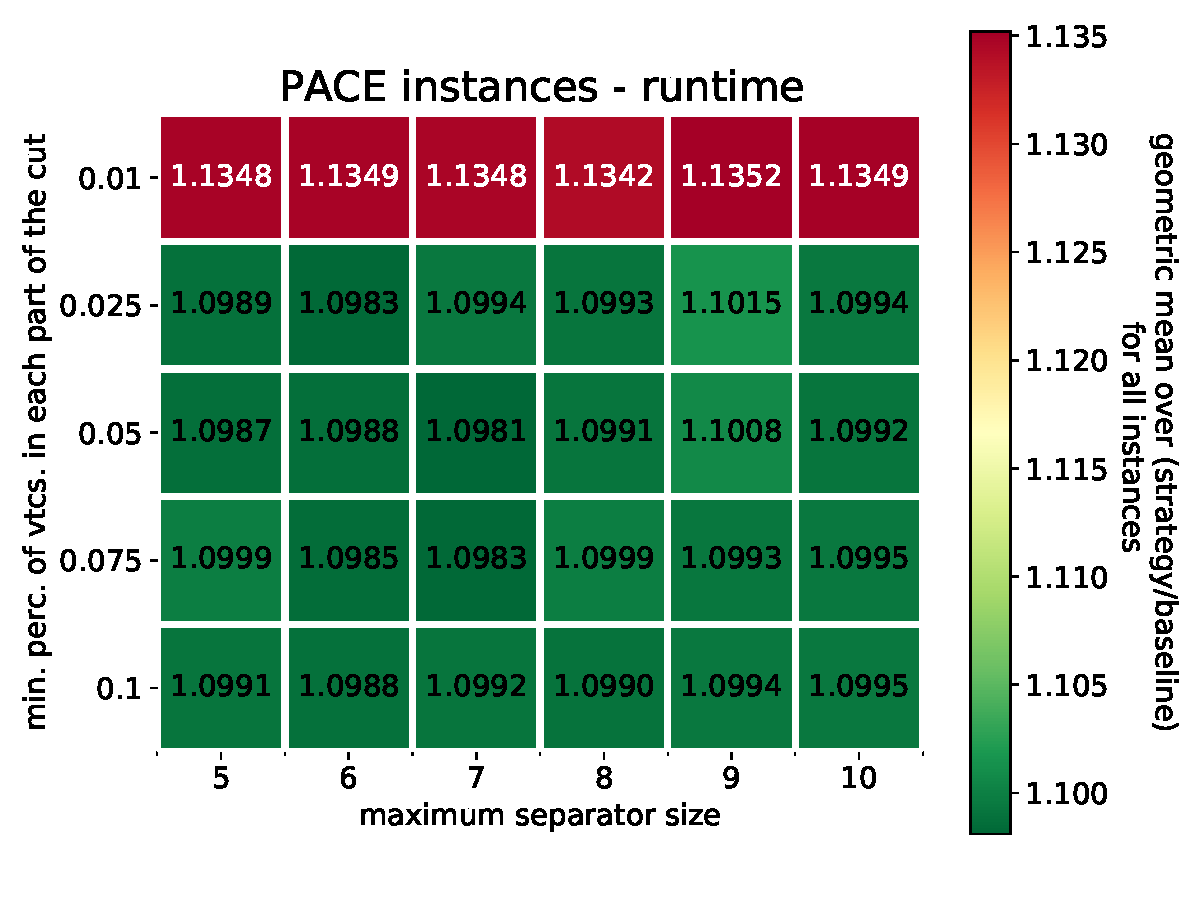
\includegraphics[width=\textwidth]{images/plots/st_tune_pace_t}
		%\caption{PACE and DIMACS - runtime}
	\end{subfigure}
	\begin{subfigure}{0.475\textwidth}
		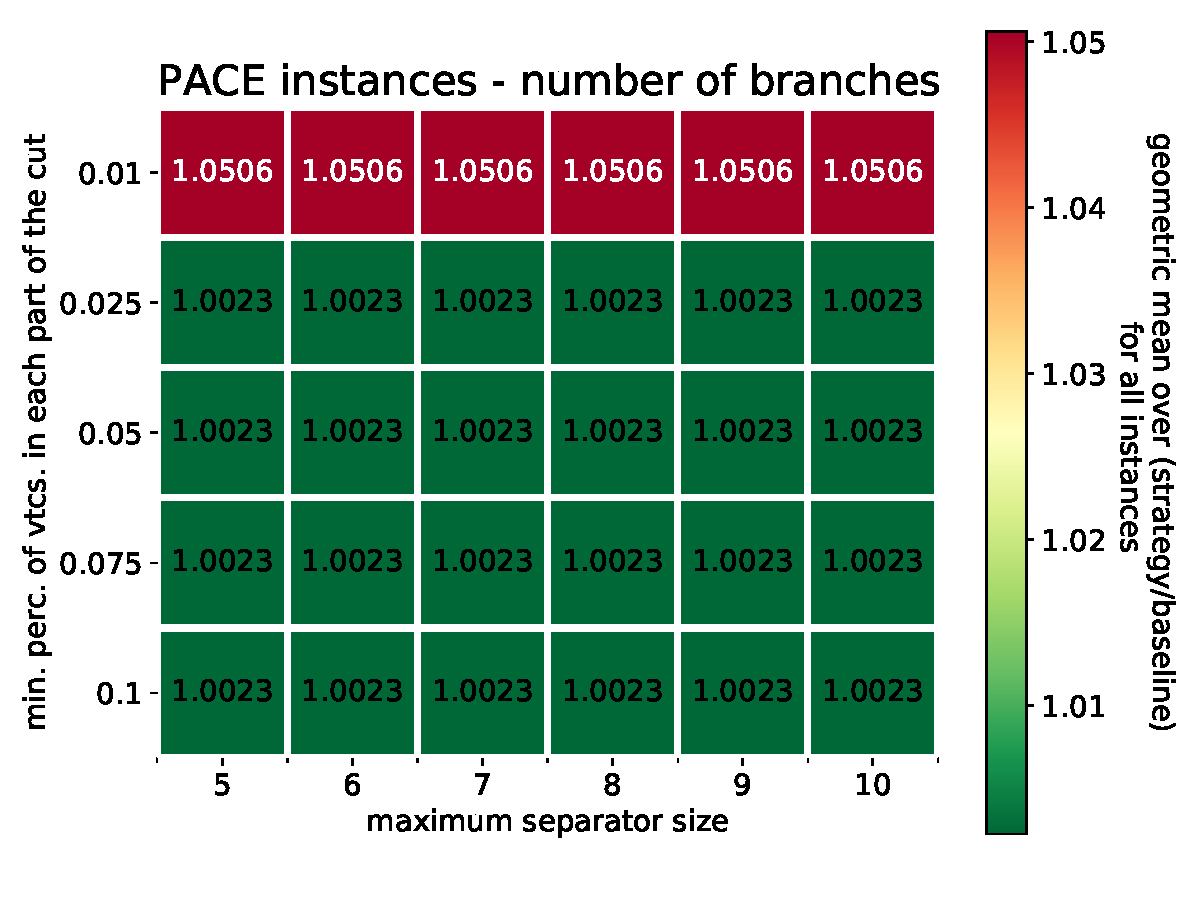
\includegraphics[width=\textwidth]{images/plots/st_tune_pace_b}
		%\caption{PACE and DIMACS - number of branches}
	\end{subfigure}
	
	\begin{subfigure}{0.475\textwidth}
		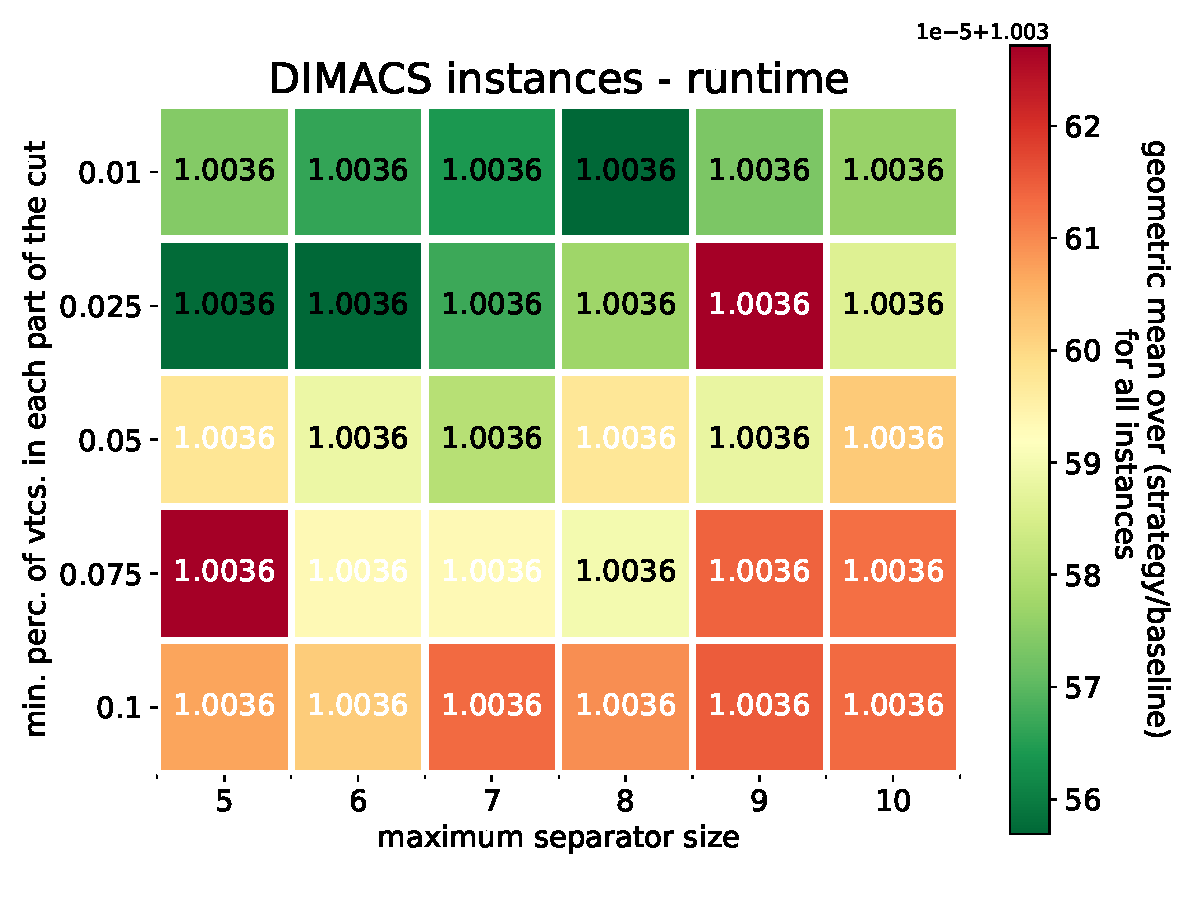
\includegraphics[width=\textwidth]{images/plots/st_tune_dimacs_t2}
		%\caption{All instances - runtime}
	\end{subfigure}
	\begin{subfigure}{0.475\textwidth}
		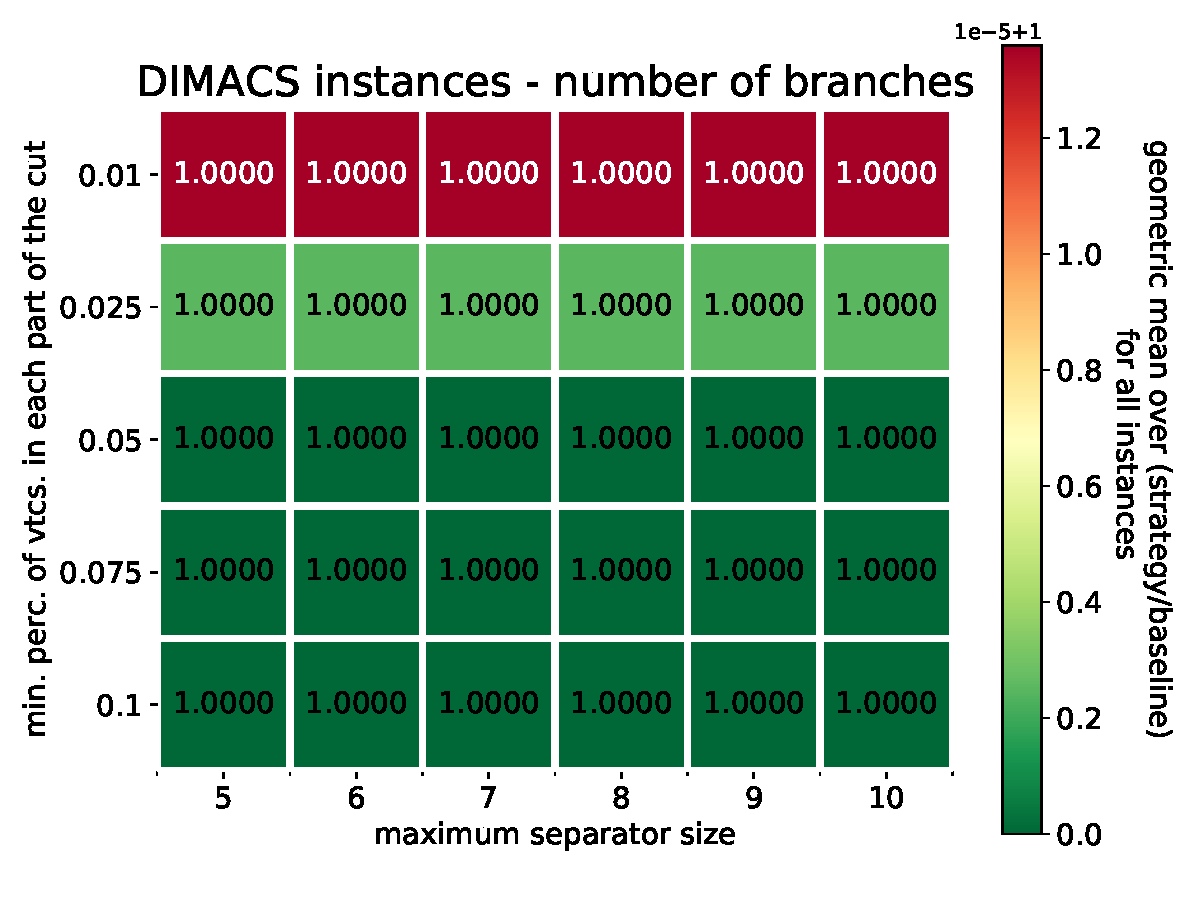
\includegraphics[width=\textwidth]{images/plots/st_tune_dimacs_b}
		%\caption{All instances - number of branches}
	\end{subfigure}
	\caption{Results from tuning the maximum separator size and the balance of an edge cut considered by the branching strategy utilizing edge cuts on PACE and DIMACS instances}	
	\label{st}
	
\end{figure}
\begin{figure}[htb!]
	\centering	
	\begin{subfigure}{0.475\textwidth}
		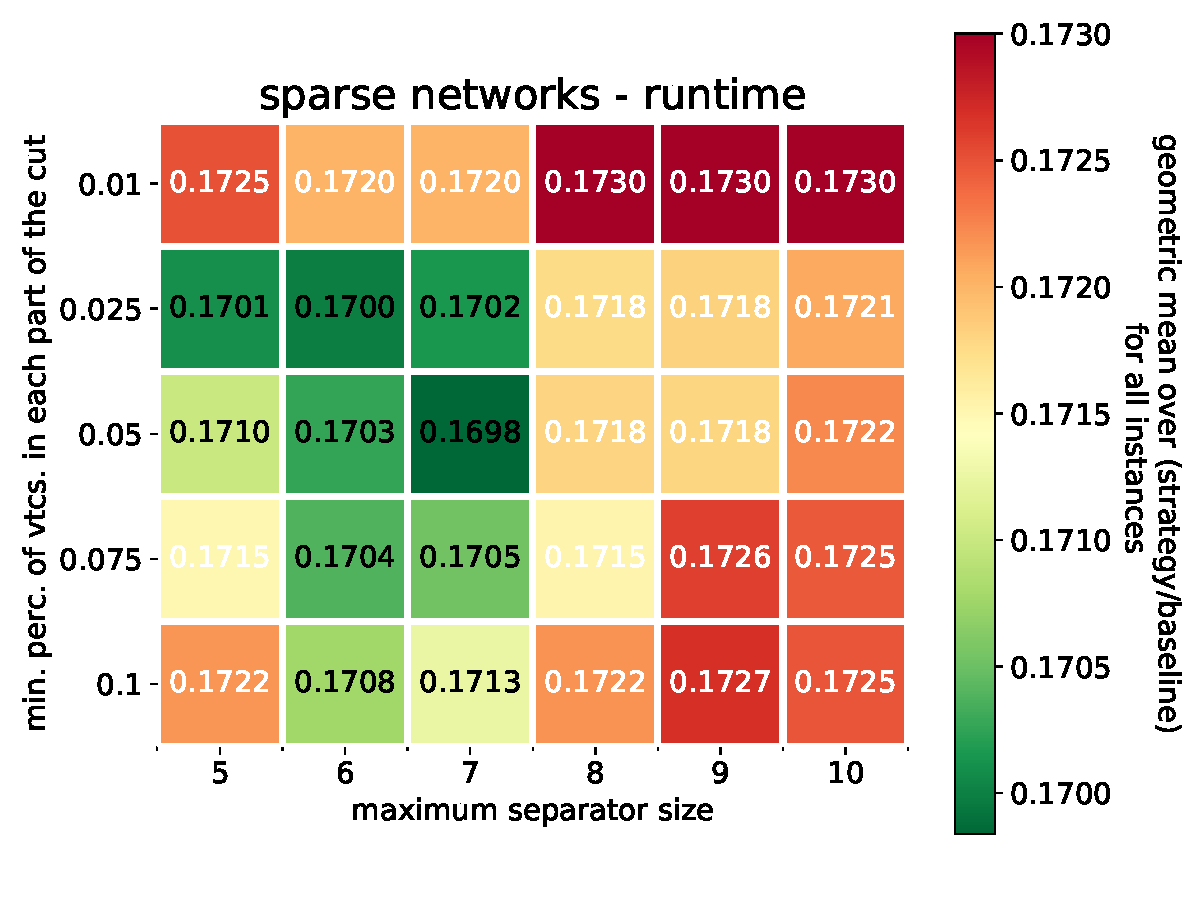
\includegraphics[width=\textwidth]{images/plots/st_tune_sn_t}
		%\caption{sparse networks - runtime}
	\end{subfigure}
	\begin{subfigure}{0.475\textwidth}
		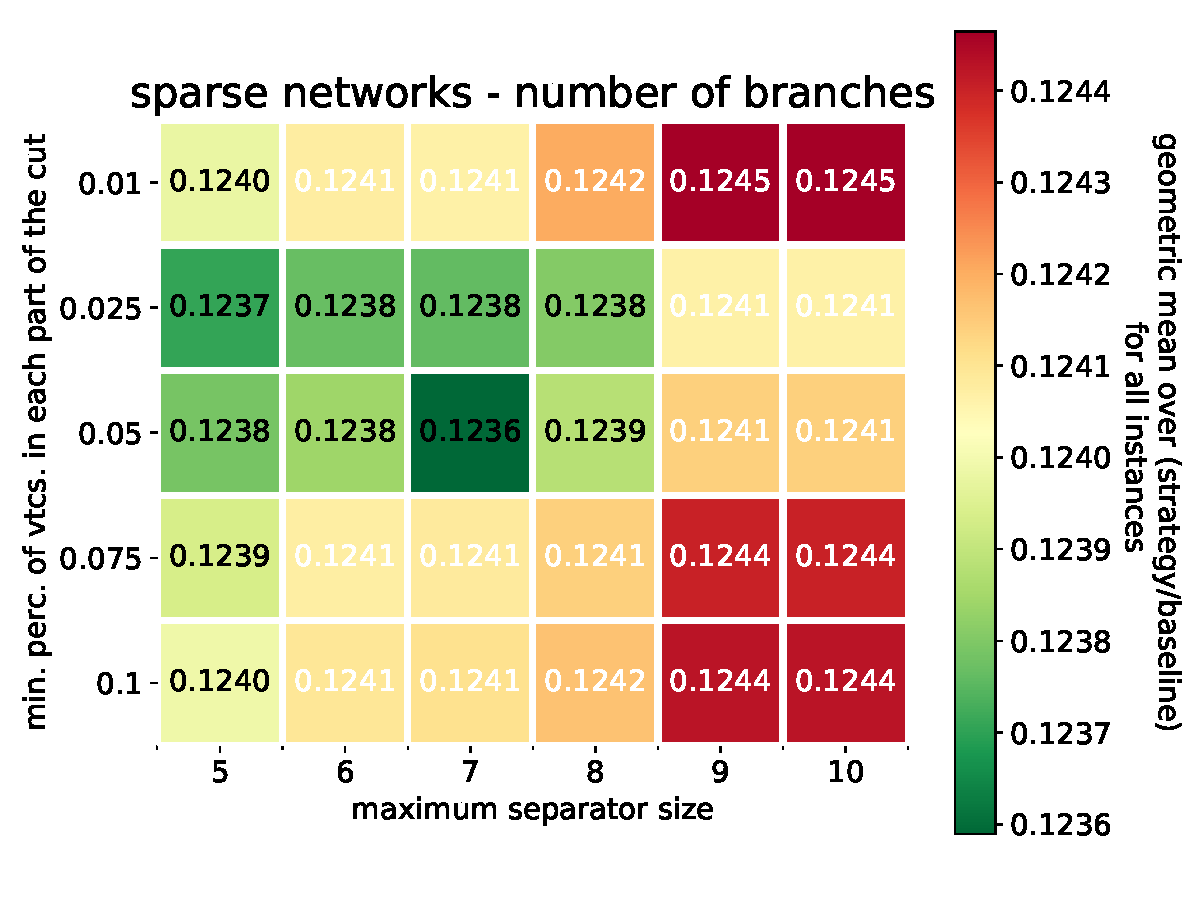
\includegraphics[width=\textwidth]{images/plots/st_tune_sn_b}
		%\caption{sparse networks - number of branches}
	\end{subfigure}
	\begin{subfigure}{0.475\textwidth}
		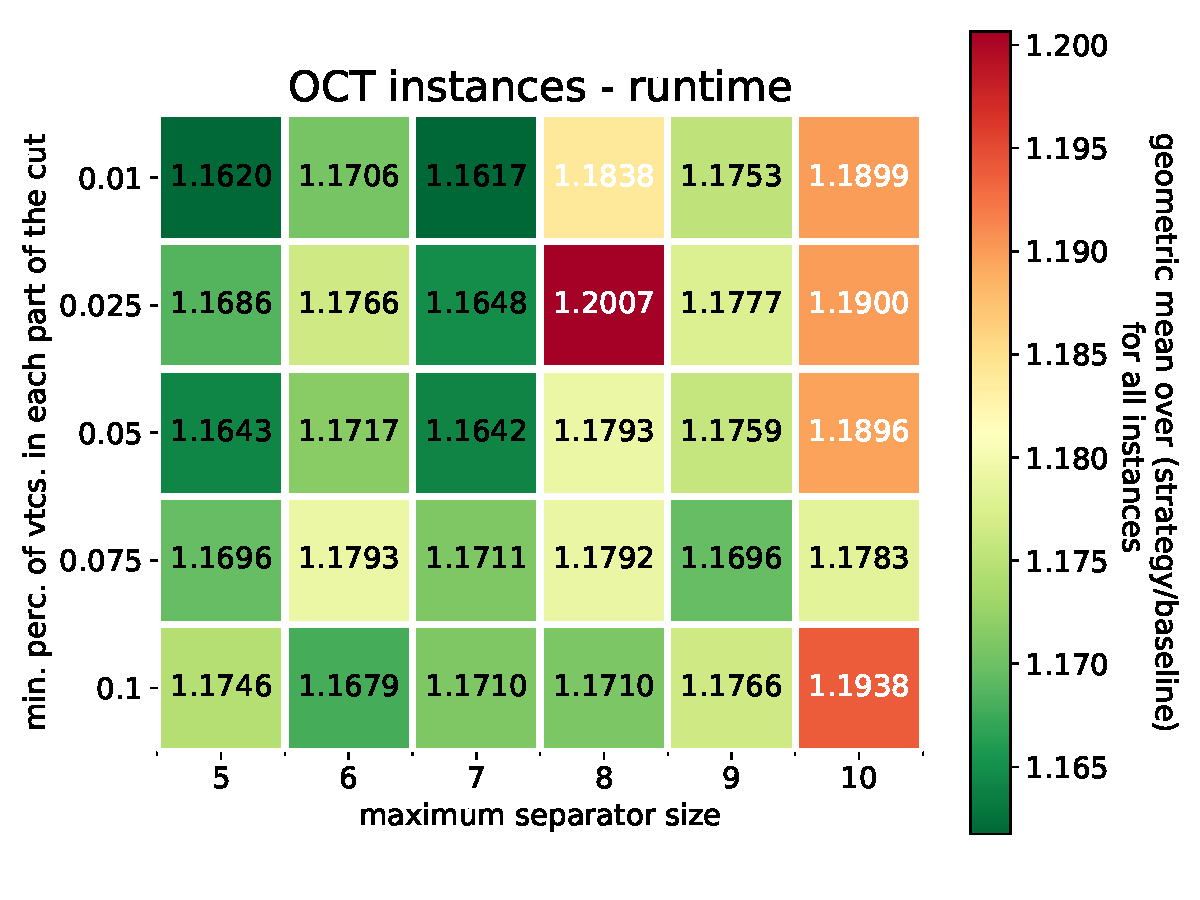
\includegraphics[width=\textwidth]{images/plots/st_tune_oct_t}
		%\caption{OCT instances - runtime}
	\end{subfigure}
	\begin{subfigure}{0.475\textwidth}
		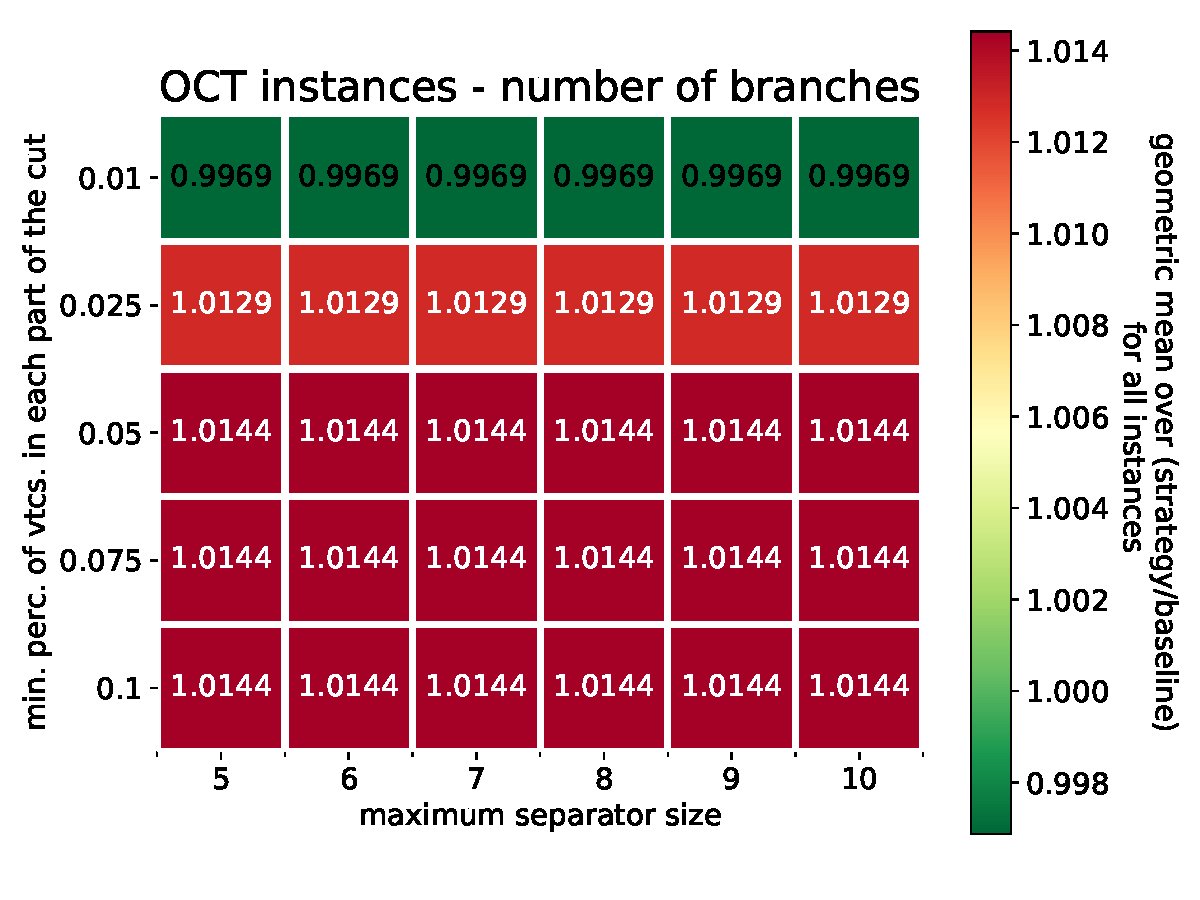
\includegraphics[width=\textwidth]{images/plots/st_tune_oct_b}
		%\caption{OCT instances - number of branches}
	\end{subfigure}
	\caption{Results from tuning the maximum separator size and the balance of an edge cut considered by the branching strategy utilizing edge cuts on OCT instances and on all instances}	
	\label{st2}
	
\end{figure}
\begin{figure}[htb!]
	\centering	
	\begin{subfigure}{0.475\textwidth}
		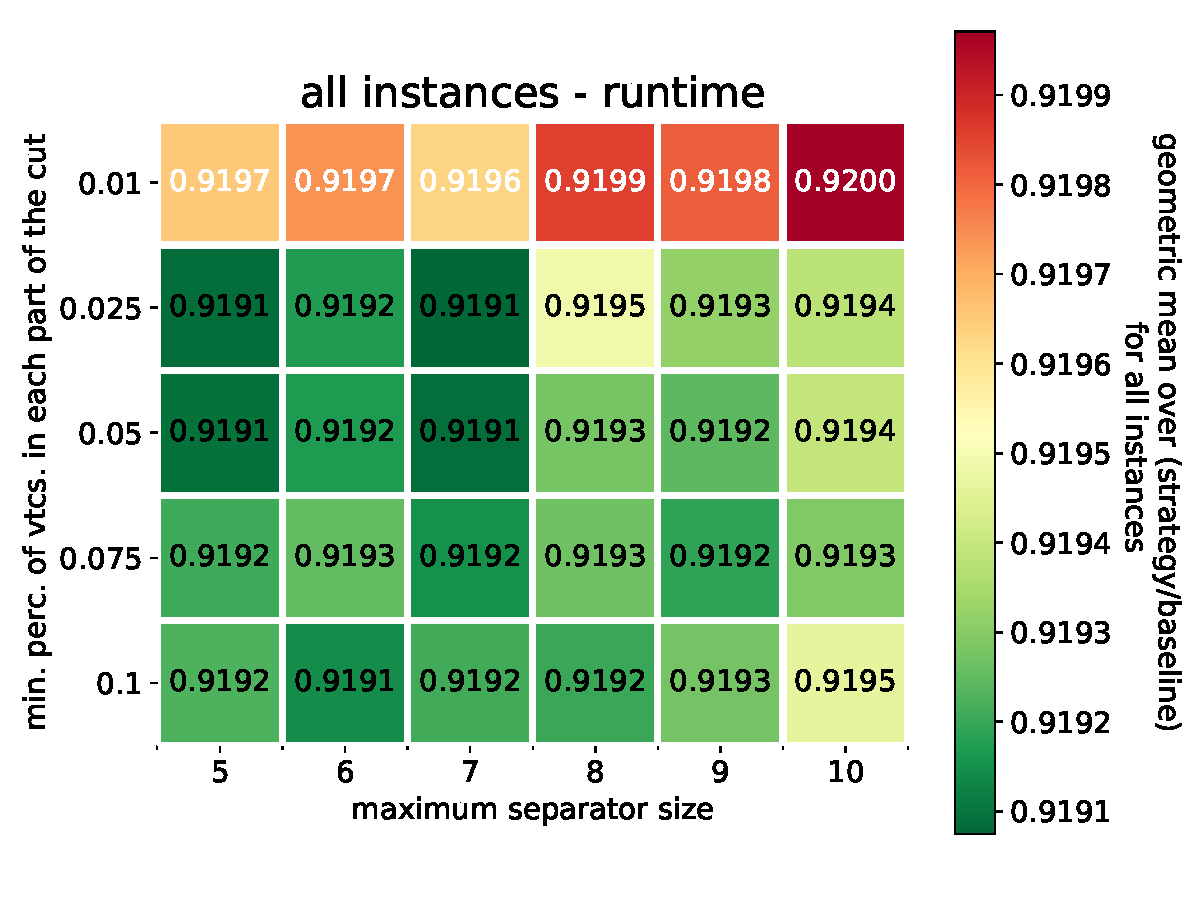
\includegraphics[width=\textwidth]{images/plots/st_tune_all_t}
		%\caption{all instances - runtime}
	\end{subfigure}
	\begin{subfigure}{0.475\textwidth}
		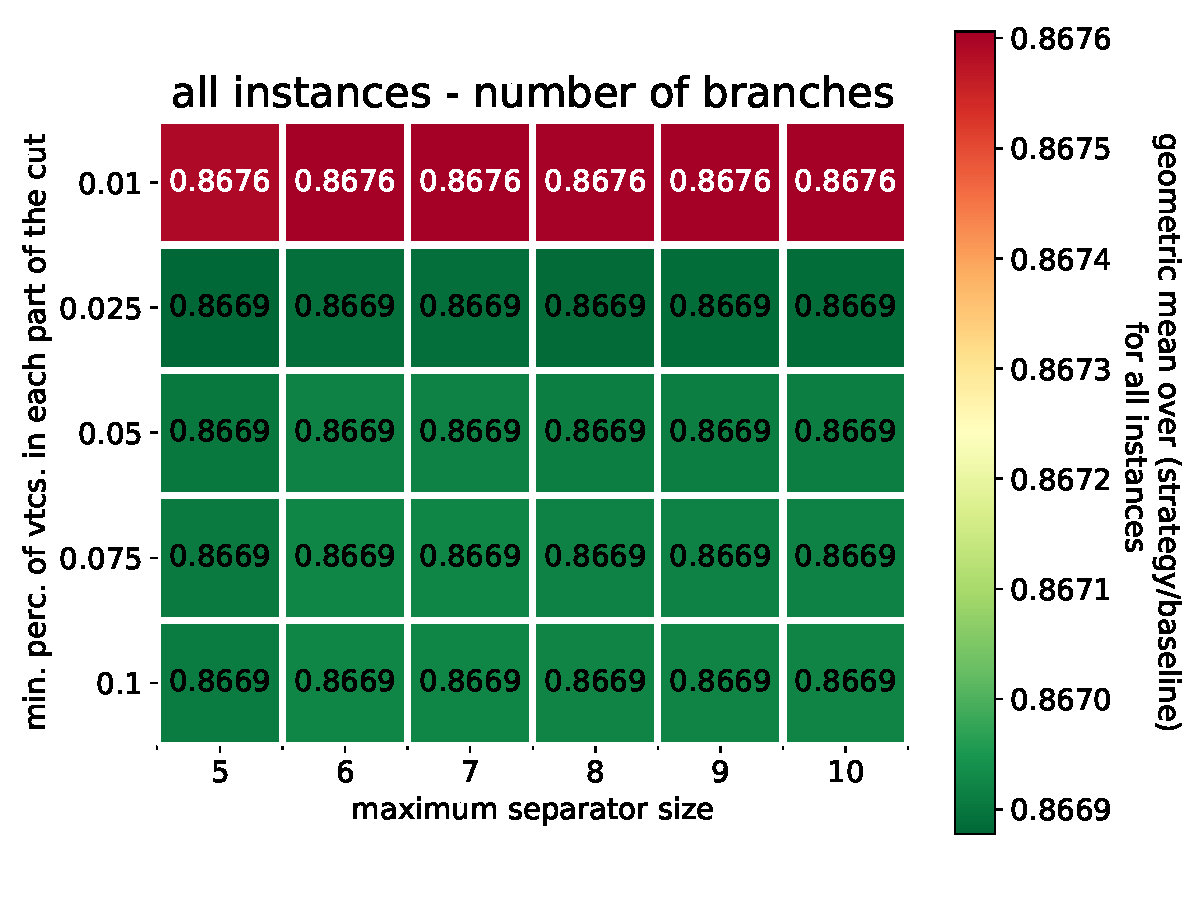
\includegraphics[width=\textwidth]{images/plots/st_tune_all_b}
		%\caption{all instances - number of branches}
	\end{subfigure}
	\caption{Results from tuning the maximum separator size and the balance of an edge cut considered by the branching strategy utilizing edge cuts on all instances}	
	\label{st3}
	
\end{figure}
\FloatBarrier
\paragraph{}
Results from tuning the third parameter, i.e. frequency cuts are being searched, are shown in Table~\ref{tab:levels1} and \ref{tab:levels2}. However, tuning the third  parameter does not give any new insight. Obviously, on sparse networks, where the branching strategy performs very well, it is advantageous to search for edge cuts in each branching step. On the other instances, however, best performance is achieved by setting the highest possible value for the third parameter, as suitable cuts are rarely found. Therefore searching for cuts with a high frequency produces unnecessary overhead. Considering all instances used for tuning, searching for edge cuts every 10 branching steps (if no suitable edge cuts are found) yields the best outcome in regards to runtime.

\begin{table}[hbt!]
	\centering
	\begin{tabular}{l|ccccc|}	  & \multicolumn{5}{c|}{Frequency of searching edge cuts} \\ \cline{2-6}
		Instances & 1 & 5 & 10 & 15 & 20\\
		\hline
		PACE & 1.1437 & 1.0933 & 1.0965 & 1.0983 & \textbf{1.0537} \\
		DIMACS & 1.1542 & 1.0564 & 1.0036 & 1.0025 & \textbf{1.0021} \\
		sparse networks & \textbf{0.0867} & 0.1239 & 0.1698 & 0.1743 & 0.1742 \\
		OCT & 1.3774 & 1.1787 & 1.1642 & 1.1571 & \textbf{1.1285} \\
		All instances & 1.2516 & 1.0271 & \textbf{0.9191} & 1.0984 & 1.0991 \\\hline
	\end{tabular}
	
	\caption{Geometric mean over the runtime relative to the default strategy with different frequencies of searching edge cuts}
	\label{tab:levels1}
	
\end{table}

\begin{table}[hbt!]
	\centering
	\begin{tabular}{l|ccccc|}	  & \multicolumn{5}{c|}{Frequency of searching edge cuts} \\ \cline{2-6}
		Instances & 1 & 5 & 10 & 15 & 20\\
		\hline
		PACE & \textbf{1.0023} & \textbf{1.0023} & \textbf{1.0023} & \textbf{1.0023} & \textbf{1.0023} \\
		DIMACS & \textbf{1.0000} & \textbf{1.0000} & \textbf{1.0000} & \textbf{1.0000} & \textbf{1.0000} \\
		sparse networks & \textbf{0.0255} & 0.0319 & 0.1236 & 0.1278 & 0.1281 \\
		OCT & \textbf{1.0144} & \textbf{1.0144} & \textbf{1.0144} & \textbf{1.0144} & \textbf{1.0144} \\
		All instances & \textbf{0.8255} & 0.8348 & 0.8669 & 0.8634 & 0.8620 \\\hline
	\end{tabular}
	
	\caption{Geometric mean over the total number of branches relative to the default strategy with different frequencies of searching edge cuts}
	\label{tab:levels2}
	
\end{table}
\subsubsection{Tuning Branching by Nested Dissection}
Next, we optimize the branching strategy based on nested dissection. We have already shown that the balance of a separator can be important for the effectiveness of a decomposing strategy. However, tuning the various settings of the actual nested dissection algorithm was out of scope for this thesis. Instead, we selected the number of recursions performed by the nested dissection algorithm and the maximum cardinality of the vertex separators at each level of recursion as parameters for tuning.

\paragraph{}
The number of recursions does not influence the sizes of the separators found at each level of recursion by the nested dissection algorithm. For this reason we decide to tune both parameters separately in order to reduce the number of experiments needed.

\paragraph{}
Since the nested dissection algorithm from the METIS library uses balanced bipartitions, the calculation of a complete nested dissection ordering using METIS requires $\mathcal{O}(\log n)$ levels of recursion where $n$ denotes the remaining number of vertices in the current graph when calculating the ordering. However, as explained in Section \ref{sec4}, it is advantageous to perform a restricted number of recursions. Therefore, we choose the number of levels of recursion from the set $\{2,3,4,5 \log{n} - 6,\log{n} - 5,\log{n}-4,\log{n}-3\}$. For the parameter relating to the maximum separator sizes we also tried constant values as well as thresholds depending on the number of vertices in the initial kernel of the instance, i.e., the graph right after the first kernelization step. Overall, we tried the following values $\{20, 30, 40, 50, 0.05n, 0.1n, 0.2n, \log n\}$.

\paragraph{}
The results of our experiments involving tuning of the number of recursions, depicted in Table \ref{tab:thresh1} an \ref{tab:thresh2}, show that the branching strategy performs best with $\log n - 5$ levels of recursion. On our tuning instances this corresponds to a range of two to four levels of recursion. However, choosing a constant number from this range performs definitely worse. A possible explanation for this is that initial kernelization often produces few relatively small connected components which are solved separately. Consequently, a branching order is calculated for each of them. Depending on the size of the components, different numbers of recursion are required to obtain optimal performance. Tuning the maximum separator size yields best results (Table \ref{tab:thresh3} and \ref{tab:thresh4}) when choosing a non constant threshold of ten percent of the remaining vertices.
\\

\begin{table}[hbt!]
	\centering
	\begin{tabular}{l|cccc|}	  & \multicolumn{4}{c|}{number of levels of recursion} \\ \cline{2-5}
		Instances & $2$ & $3$ & $4$ & $5$ \\
		\hline
		PACE & 16.1889 & 16.4489 & 12.6748 & 21.0732 \\
		DIMACS & 1.2103 & 1.2418 & 1.1844 & 1.1287  \\
		sparse networks & 1.5532 & 1.6651 & 1.4912 & 1.7683  \\
		OCT & 1.1662 & \textbf{1.1229} & 1.2173 & 1.2870  \\
		All & 2.5410 & 2.5717 & 2.3286 & 2.8669 \\ \hline \hline
		& \multicolumn{4}{c|}{number of levels of recursion} \\ \cline{2-5}
		Instances & $\log n -6$ & $\log n -5$ & $\log n -4$ & $\log n -3$ \\
		\hline
		PACE & 12.5689 & \textbf{10.4004} & 15.6870 & 13.0480  \\
		DIMACS & \textbf{1.0235} & 1.2107 & 1.1968& 1.1780  \\
		sparse networks & 1.5603 & \textbf{1.3335} & 1.4517 & 1.6611  \\
		OCT & 1.1407 & 1.1254 & 1.3410 & 1.2222  \\
		All & 2.2073 & \textbf{2.0773} & 2.5841 & 2.3791  \\ \hline
		
	\end{tabular}
	\caption{Geometric mean over the runtime relative to the default strategy with different numbers of levels of recursion}
	\label{tab:thresh1}
	
\end{table}

\begin{table}[hbt!]
	\centering
	\begin{tabular}{l|cccc|}	  & \multicolumn{4}{c|}{number of levels of recursion} \\ \cline{2-5}
		Instances & $2$ & $3$ & $4$ & $5$ \\
		\hline
		PACE & 7.9015 & 7.9533 & 6.0542 & 10.4971 \\
		DIMACS & 1.0416 & 1.0611 & 0.9682 & 0.9490  \\
		sparse networks & 1.4704 & 1.6043 & 1.4943 & 1.6226  \\
		OCT & 1.2415 & 1.1823 & 1.3472 & 1.3710  \\
		All & 1.9675 & 1.9983 & 1.8537 & 2.1698 \\ \hline \hline
		& \multicolumn{4}{c|}{number of levels of recursion} \\ \cline{2-5}
		Instances & $\log n -6$ & $\log n -5$ & $\log n -4$ & $\log n -3$ \\
		\hline
		PACE & 6.0542 & \textbf{4.8960} & 7.6291 & 6.2406  \\
		DIMACS & \textbf{0.8726} & 1.0447 & 1.0301 & 0.9917  \\
		sparse networks & 1.5305 & \textbf{1.3441} & 1.3463 & 1.5603  \\
		OCT & \textbf{1.1689} & 1.1816 & 1.4252 & 1.2448  \\
		All & 1.7576 & \textbf{1.6880} & 1.9705 & 1.8621  \\ \hline
		
	\end{tabular}
	\caption{Geometric mean over the total number of branches relative to the default strategy with different numbers of levels of recursion}
	\label{tab:thresh2}
	
\end{table}

\begin{table}[hbt!]
	\centering
	\begin{tabular}{l|cccc|}	  & \multicolumn{4}{c|}{maximum separator size at each recursion} \\ \cline{2-5}
		Instances & $20$ & $30$ & $40$ & $50$ \\
		\hline
		PACE & 16.0360 & 11.3461 & 10.6191 & 13.3114  \\
		DIMACS & \textbf{1.0136} & 1.2107 & 1.3165 & 1.3230  \\
		sparse networks & 1.6152 & 1.5372 & 1.5118 & 1.6392 \\
		OCT & 1.1177 & 1.1194 & \textbf{1.1167} & 1.1488 \\
		All & 2.3281 & 2.2053 & 2.2039 & 2.2811  \\ \hline \hline
		Instances & $\log n$ & $0.005n$ & $0.1n$ & $0.2n$ \\
		\hline
		PACE & 13.9448 & 23.3915 & \textbf{10.4004} & 15.7568  \\
		DIMACS & 1.1175 & 1.1507 & 1.2107 & 1.1506  \\
		sparse networks & 1.4890 & 1.3571 & 1.3335 & 1.3337 \\
		OCT & 1.1262 & 1.1346 & 1.1254 & 1.1197  \\
		All & 2.2610 & 2.5373 & \textbf{2.0773} & 2.2811  \\ \hline
	\end{tabular}
	\caption{Geometric mean over the runtime relative to the default strategy with different maximum separator size}
	\label{tab:thresh3}
	
\end{table}

\begin{table}[hbt!]
	\centering
	\begin{tabular}{l|cccc|}	  & \multicolumn{4}{c|}{maximum separator size at each recursion} \\ \cline{2-5}
		Instances & $20$ & $30$ & $40$ & $50$ \\
		\hline
		PACE & 7.8498 & 5.3488 & \textbf{4.7668} & 6.3484 \\
		DIMACS & \textbf{0.8196} & 1.0447 & 1.1176 & 1.1280  \\
		sparse networks & 1.6077 & 1.5308 & 1.5115 & 1.6388 \\
		OCT & \textbf{1.1816} & \textbf{1.1816} & \textbf{1.1816} & \textbf{1.1816} \\
		All & 1.8701 & 1.7838 & 1.7563 & 1.9322  \\ \hline \hline
		Instances & $\log n$ & $0.005n$ & $0.1n$ & $0.2n$ \\
		\hline
		PACE & 6.6870 & 11.8011 & 4.8960 & 7.7225 \\
		DIMACS & 0.8651 & 0.9850 & 1.0447 & 0.8950  \\
		sparse networks & 1.4873 & 1.3499 & \textbf{1.3441} & 1.3341 \\
		OCT & \textbf{1.1816} & \textbf{1.1816} & \textbf{1.1816} & \textbf{1.1816}  \\
		All & 1.7863 & 2.0761 & \textbf{1.6880} & 1.8174  \\ \hline
	\end{tabular}
	\caption{Geometric mean over the total number of branches relative to the default strategy with different maximum separator size}
	\label{tab:thresh4}
	
\end{table}


\subsubsection{Tuning Branching Based on Reduction Rules}

Finally, we optimize the branching strategies utilizing reduction rules (i.e., first four branching strategies in Section \ref{red_strats}). Those strategies only have one tuning parameter, which is the minimum degree required in order for a vertex to be considered for branching by the respective branching strategy. In general, the degree distribution in a graph depends on the graph class and the size of the graph. Furthermore, applying dominance, unconfined or twin reduction, respectively, only reduces a constant number of vertices. Thus, we do not use a fixed threshold. Instead, our strategies consider vertices whose degrees differ from the maximum degree of the current graph by a certain constant value at the time of branching. We choose the concrete values from the set $\{1,2,3,4\}$. The results of tuning experiments are shown in Tables \ref{tab:tune1} to \ref{tab:tune4}. They suggest that the branching strategies based on dominance and unconfined reduction perform best when only vertices with degree greater or equal one less than the current maximum degree are considered. This was expected, as both unconfined and dominance reduction rule each eliminate one vertex of the graph. The branching strategy based on the twin reduction achieves the best results when choosing $2$ for the value of the tuning parameter (see Table \ref{tab:tune2} and \ref{tab:tune4}). Applying twin reduction rule reduces either four or five vertices from the graph. Using the branching strategy based on funnel reduction, best results are obtained with $2$ as value for the tuning parameter.

\begin{table}[hbt!]
	\centering
	\begin{tabular}{l|cccc|cccc|}	  & \multicolumn{4}{c|}{almost dominance} & \multicolumn{4}{c|}{almost unconfined} \\
		Instances & 0 & 1 & 2 & 3 & 0 & 1 & 2 & 3 \\ \hline
		PACE & 1.0118 & \textbf{0.9889} & 1.0010 & 1.0059 & $1.0358$ & \textbf{1.0216} & $1.0306$ & $1.0449$ \\
		DIMACS & 1.0189 & 1.0225 & 1.0216 & \textbf{1.0096} & 0.9768 & 0.9767 & 0.9744 & \textbf{0.9405}  \\
		sparse Networks & 0.9560 & \textbf{0.9399} & 0.9590 & 1.0667 & 0.9739 & \textbf{0.9589} & 0.9754 & 1.1130  \\
		OCT & 1.0721 & \textbf{1.0342} & 1.0570 & 1.0382 & 1.0747 & 1.0680 & 1.0612 & \textbf{1.0486} \\
		All & 1.0230 & \textbf{1.0057} & 1.0165 & 1.0197 & 1.0218 & \textbf{1.0135} & 1.0161 & 1.0207  \\
	\end{tabular}
	\caption{Geometric mean over the runtime relative to the default strategy with different thresholds for the minimum degree so that a vertex is considered for branching}
	\label{tab:tune1}
	
\end{table}

\begin{table}[hbt!]
	\centering
	\begin{tabular}{l|cccc|cccc|}	  & \multicolumn{4}{c|}{almost dominance} & \multicolumn{4}{c|}{almost unconfined} \\
		Instances & 0 & 1 & 2 & 3 & 0 & 1 & 2 & 3 \\ \hline
		PACE & 1.0003 & 0.9897 & \textbf{0.9875} & 0.9931 & 1.0016 & \textbf{0.9962} & 1.0027 & 1.0225\\
		DIMACS & 0.9949 & 1.0009 & 1.0010 & \textbf{0.9909} & 0.9916 & 0.9822 & 0.9791 & \textbf{0.9659}  \\
		sparse Networks & 1.0682 & \textbf{1.0494} & 1.1361 & 1.3363 & 1.0686 & \textbf{1.0472} & 1.1518 & 1.4241  \\
		OCT & 1.0106 & 1.0084 & 1.0075 & \textbf{1.0060} & 1.0038 & 0.9848 & 0.9847 & \textbf{0.9547} \\
		All & 1.0077 & \textbf{1.0032} & 1.0099 & 1.0245 & 1.0055 & \textbf{0.9941} & 1.0046 & 1.0207  \\
	\end{tabular}
	\caption{Geometric mean over the number of branches relative to the default strategy with different thresholds for the minimum degree so that a vertex is considered for branching}
	\label{tab:tune3}
	
\end{table}
\begin{table}[hbt!]
	\centering
	\begin{tabular}{l|cccc|cccc|}	  & \multicolumn{4}{c|}{almost twins} & \multicolumn{4}{c|}{almost funnels} \\
		Instances & 0 & 1 & 2 & 3 & 0 & 1 & 2 & 3 \\ \hline
		PACE & 0.9767 & 0.9841 & \textbf{0.9617} & 0.9856 & 1.0152 & 0.9532 & \textbf{0.9148} & 0.9634 \\		
		DIMACS & 0.9424 & 0.9710 & \textbf{0.9346} & 0.9735 & 0.9870 & 1.0236 & \textbf{0.9836} & 1.0121 \\		
		sparse Networks & 0.9394 & \textbf{0.9382} & 0.9387 & 0.9429 & 0.9986 & \textbf{0.9724} & 0.9810 & 1.1417  \\		
		OCT & \textbf{0.9903} & 1.0031 & 0.9969 & 0.9983 & 1.1523 & 1.1111 & 1.1041 & \textbf{1.0731} \\
		All & 0.9664 & 0.9805 & \textbf{0.9602} & 0.9811 & 1.0377 & 1.0129 & \textbf{0.9857} & 1.0204  \\
	\end{tabular}
	\caption{Geometric mean over the runtime relative to the default strategy with different thresholds for the minimum degree so that a vertex is considered for branching}
	\label{tab:tune2}
	
\end{table}

\begin{table}[hbt!]
	\centering
	\begin{tabular}{l|cccc|cccc|}	  & \multicolumn{4}{c|}{almost twins} & \multicolumn{4}{c|}{almost funnels} \\
		Instances & 0 & 1 & 2 & 3 & 0 & 1 & 2 & 3 \\ \hline
		PACE & 1.0025 & 1.0025 & 1.0023 & \textbf{1.0022} & 0.9649 & 0.8973 & \textbf{0.8924} & 0.9247 \\		
		DIMACS & \textbf{0.9957} & \textbf{0.9957} & \textbf{0.9957} & \textbf{0.9957} & 0.9984 & 0.9963 & 0.9919 & \textbf{0.9815} \\		
		sparse Networks & 1.0791 & 1.0745 & \textbf{1.0659} & \textbf{1.0659} & 1.0697 & \textbf{1.0143} & 1.0468 & 1.3213  \\
		OCT & 1.0094 & 1.0059 & \textbf{1.0050} & 1.0057 & 1.0016 & 0.9320 & \textbf{0.9101} & 0.9274\\		
		All & 1.0094 & 1.0081 & \textbf{1.0069} & 1.0072 & 0.9934 & 0.9447 & \textbf{0.9388} & 0.9743  \\
	\end{tabular}
	\caption{Geometric mean over the number of branches relative to the default strategy with different thresholds for the minimum degree so that a vertex is considered for branching}
	\label{tab:tune4}
	
\end{table}



\subsection{Evaluation} \label{eval}
Having tuned the branching strategies, we can now evaluate their effectiveness. To compare different strategies we utilize performance plots introduced in \cite{performance}. These plots depict the performance of a strategy in relation to the best strategy on a per instance basis. The y-axis shows $1-\text{(best strategy/strategy)}$. For each branching strategy, these values are sorted in decreasing order. Smaller values indicate performance is closer to the best strategy, whereas values close to one show that the strategy performed considerably worse. A value of zero signifies the strategy performed best on an instance. Timeouts are placed above one. We use a square root scale in order to increase the visible details in the area close to zero. 

\subsubsection{Evaluation of Decomposing Branching Strategies}
We start by comparing the strategies following our first approach which is decomposing the graph by branching. Results of testing these strategies are plotted in Figures \ref{11} to \ref{22}. Results show that for most of the PACE and DIMACS instances the branching strategy utilizing articulation points turns out to be slower than the default branching strategy. The same is true for the graphs obtained from the OCT instances. The reason for this is that almost no articulation points are found on these graphs. Consequently, default branching is applied anyway, resulting in unnecessary overhead by searching for articulation points in the first place. Nevertheless, there are two outliers among the sparse networks, where branching on articulation points significantly outperforms the default branching strategy. The most notable of these exceptions is the \texttt{web-Stanford} instance (sparse network), which is intractable on our machine within 24 hours using the default branching strategy. The same instance, however, is solved in less than 20 seconds utilizing branching on articulation points, although only 35 articulation points are discovered throughout the whole run. In fact, 34 of the 35 articulation points are found at recursion depths lower than 12. This supports the hypothesis that decompositions performed at early stages of the algorithm are highly effective. Furthermore, articulation points can be found very efficiently in linear time using a DFS scheme. Thus, the additional overhead needed for searching articulation points, even if none exists, is very small. In our experiments this branching strategy is about five percent slower on average than the default branching strategy, if almost no articulation points are found. Obviously, the total number of branching steps needed to solve the respective instances is almost equal to default branching. 

\paragraph{}
Similar to branching on articulation points, the branching strategy using edge cuts performs worse than the default branching strategy on PACE and DIMACS instances as well as on the graphs obtained from OCT instances. Our experiments show that cuts suitable for branching are rarely found. Thus, the fallback strategy is getting applied almost always, which results in a nearly equal number of branches as with the default strategy, i.e., within a range of plus minus one percent relative to the default strategy. However, the overhead of calculating the edge cut is considerably higher than detecting articulation points. Using the configuration obtained by parameter tuning, solving PACE and DIMACS instances takes about seven percent longer on average than with the default branching strategy. OCT instances require about thirteen percent more runtime on average. Nevertheless, just as branching on articulation points, this strategy performs considerably well on two of the sparse networks. For instance, solving the \texttt{web-Stanford} instance requires about five minutes using this branching strategy. That is because a lot of small and reasonable well balanced cuts are found on those instances which are therefore easily decomposable. However, branching on articulation points overall performs better, since less overhead is produced.
\paragraph{}

Using the branching strategy based on nested dissection yields mixed results in our experiments. On the PACE instances, this strategy performs a lot worse than default branching and the other two strategies examined so far had done. The runtime solving PACE instances is about ten times higher on average than with using the default strategy. However, there is one outlier for which this branching strategy gives the best result compared to all branching strategies. Furthermore, nested dissection branching performs slightly better than default on DIMACS instances. Eleven of the fifteen benchmark instances can be solved quicker using the branching strategy based on nested dissection. Contrary, there are also two DIMACS instances where this strategy is up to five times slower than default branching. Overall, the performance on DIMACS instances is surprising as both, branching on articulation points and branching on edge cuts, each perform more or less equal on PACE and DIMACS instances. Unfortunately, we do not have an explanation for this. On sparse networks, the results are mixed. For two of the instances nested dissection branching yields better runtimes than the default branching strategies. On one of them it even performs best out of all branching strategies. However, on the remaining three instances this branching strategy performs very badly.

\paragraph{}
Summarizing, the results so far show that our approach to decompose instances by branching is often effective on sparse networks. The reason for this is that those instances are easily decomposable. Also, sparse networks have a low average degree. Thus, branching on vertices of maximum degree becomes ineffective as soon as all vertices of high degree have been removed. Unfortunately, this approach does not work on denser graphs. The experiments also indicate that decomposing the graph at an early stage of the algorithm is much more powerful than in later stages.

\begin{figure}[hbt!]
	\begin{subfigure}{1\textwidth}
		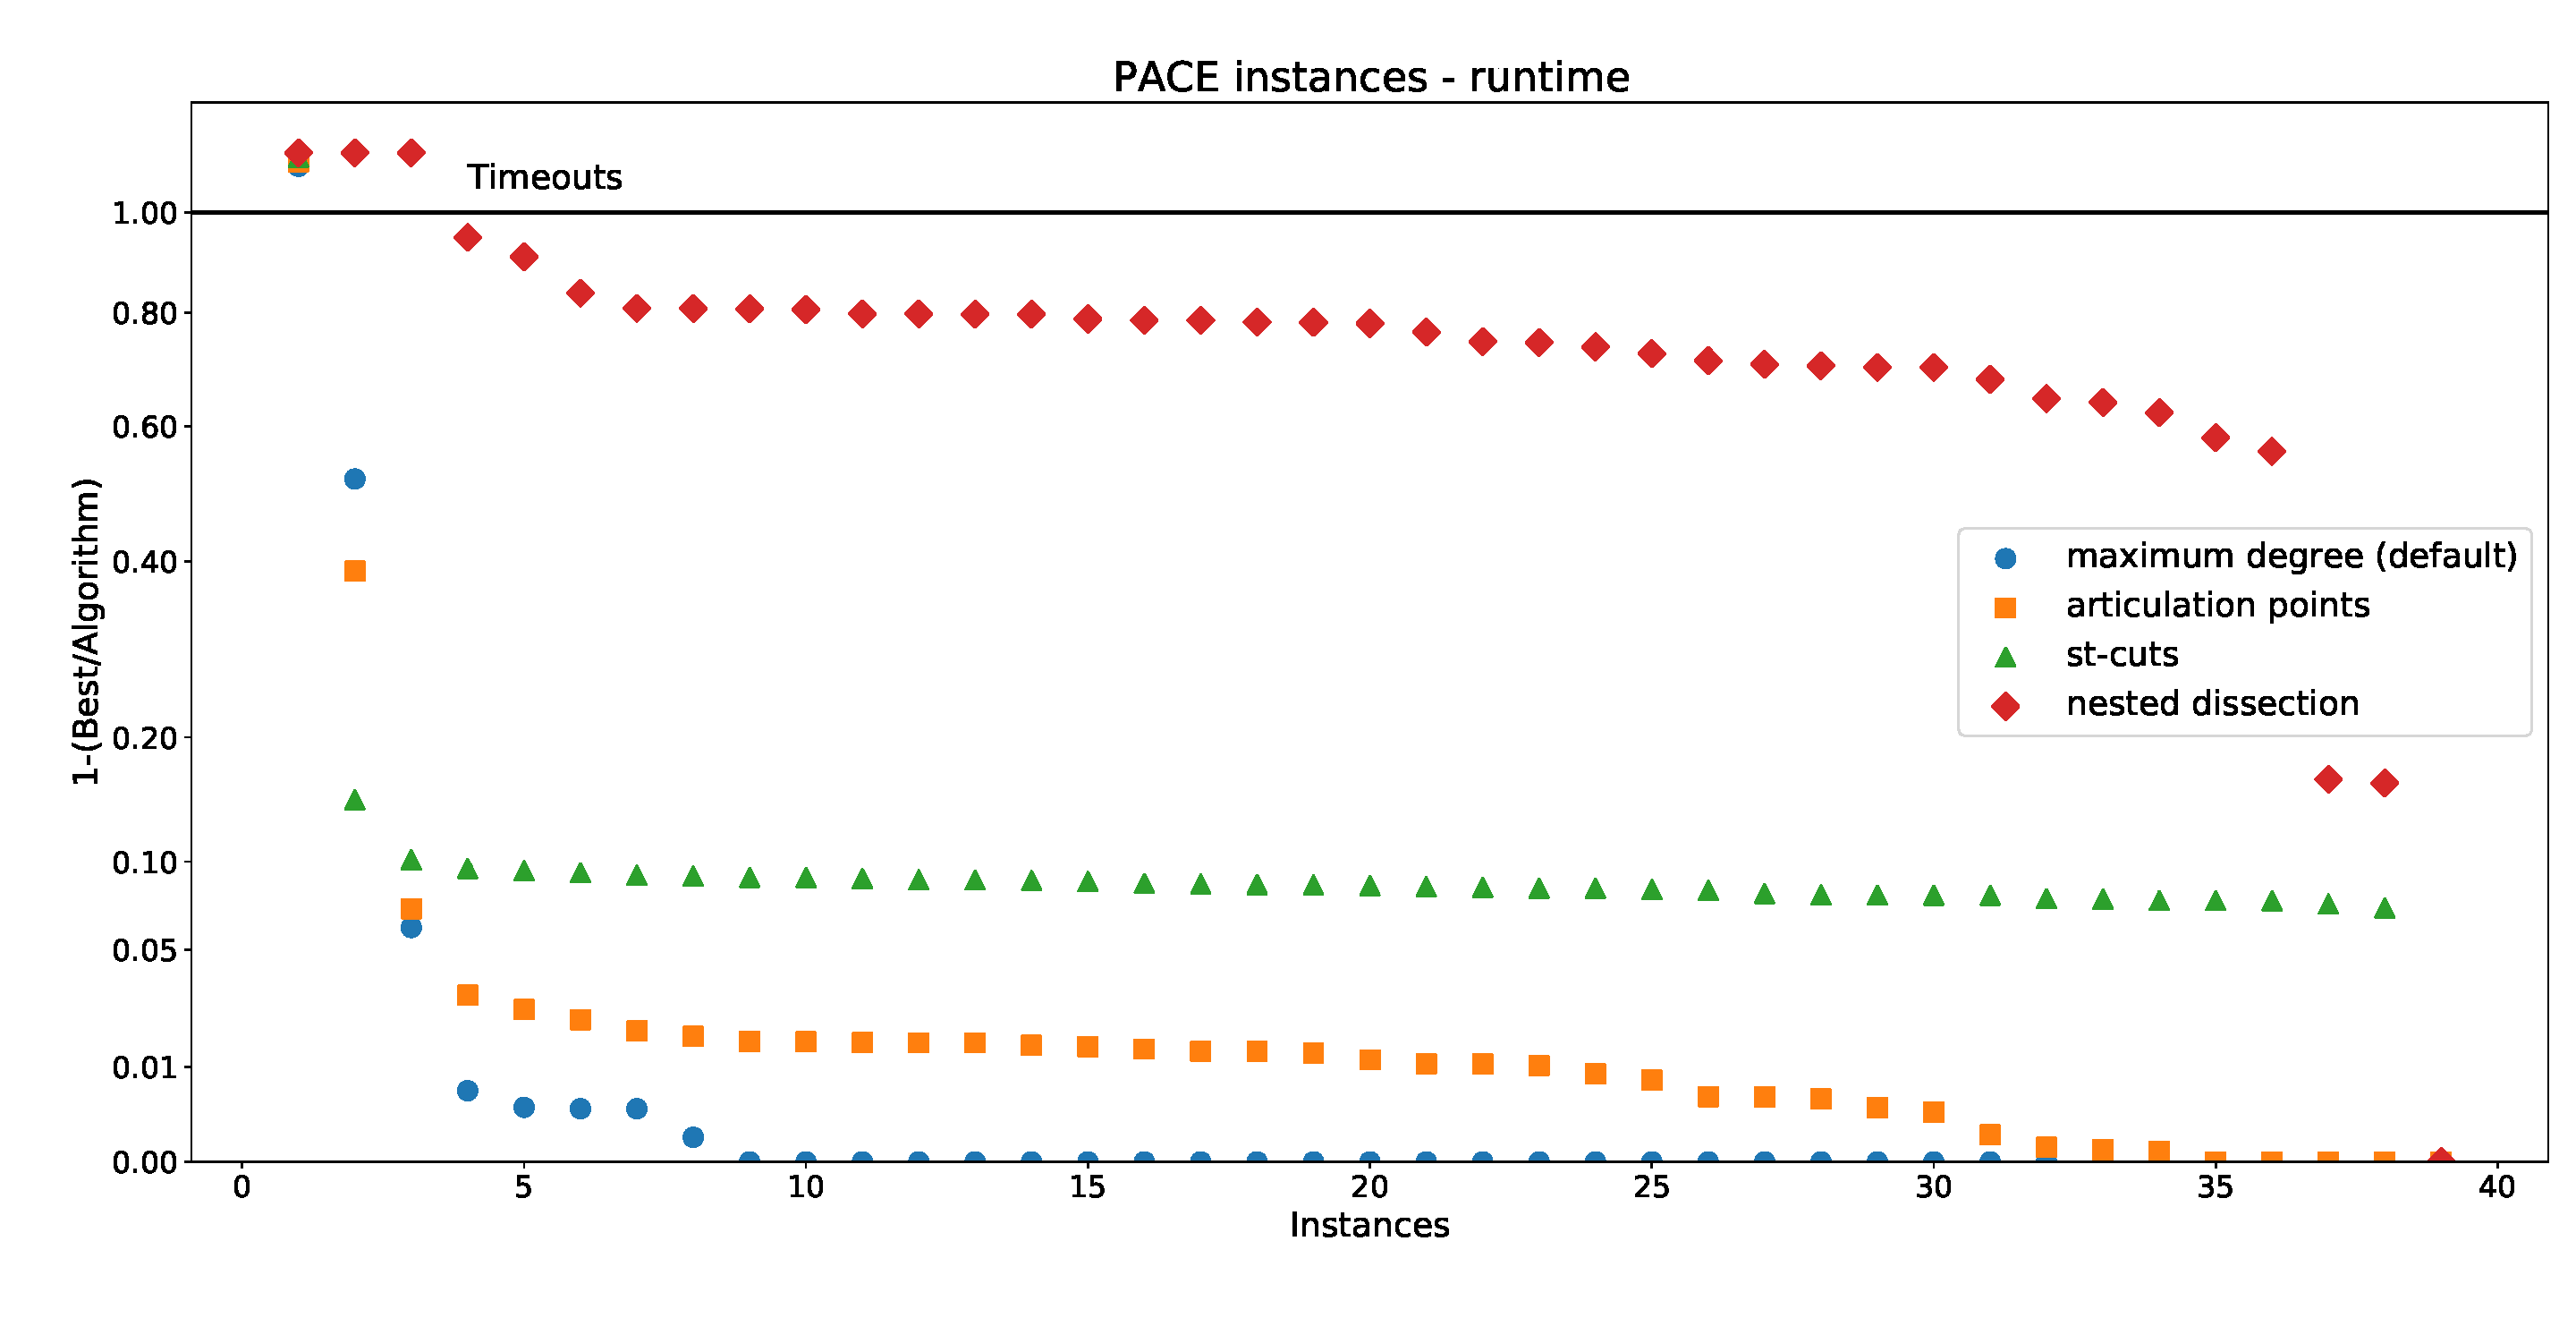
\includegraphics[width=\textwidth]{images/plots/a1_pace_t}
		\caption{runtime}
	\end{subfigure}
	\begin{subfigure}{1\textwidth}
		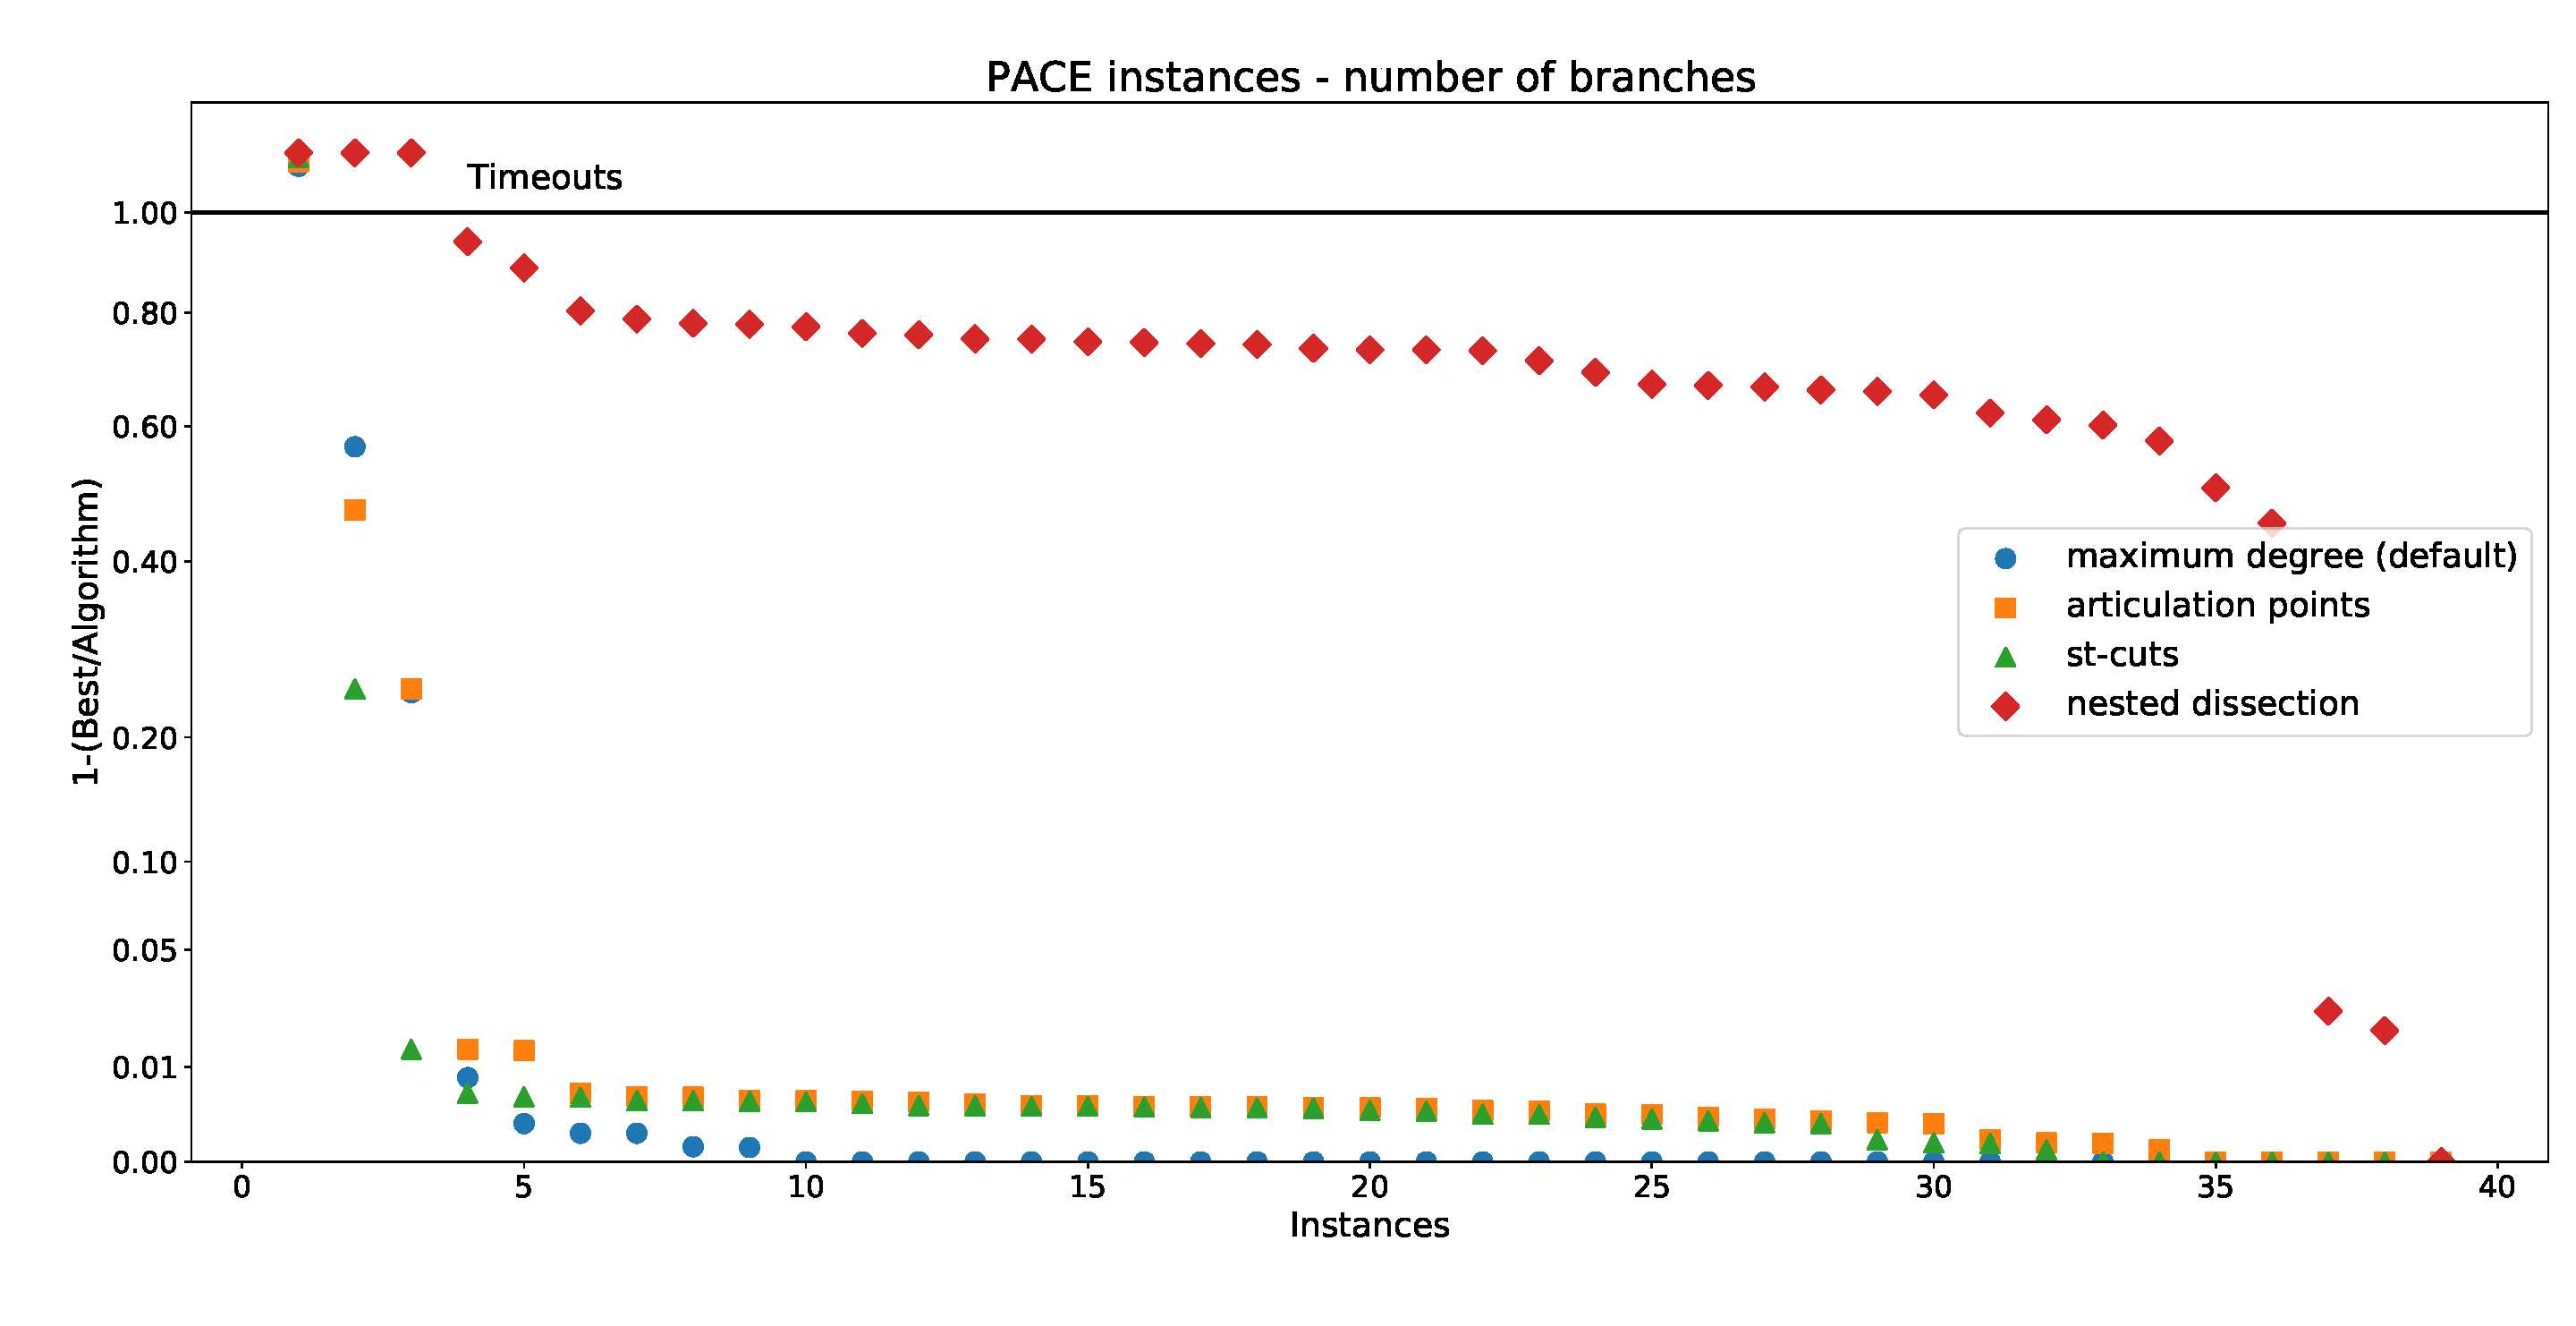
\includegraphics[width=\textwidth]{images/plots/a1_pace_b}
		\caption{number of branches}
	\end{subfigure}
	\caption{Performance plots of decomposing branching strategies on PACE instances}
	\label{11}
\end{figure}
\begin{figure}[hbt!]
	\begin{subfigure}{1\textwidth}
		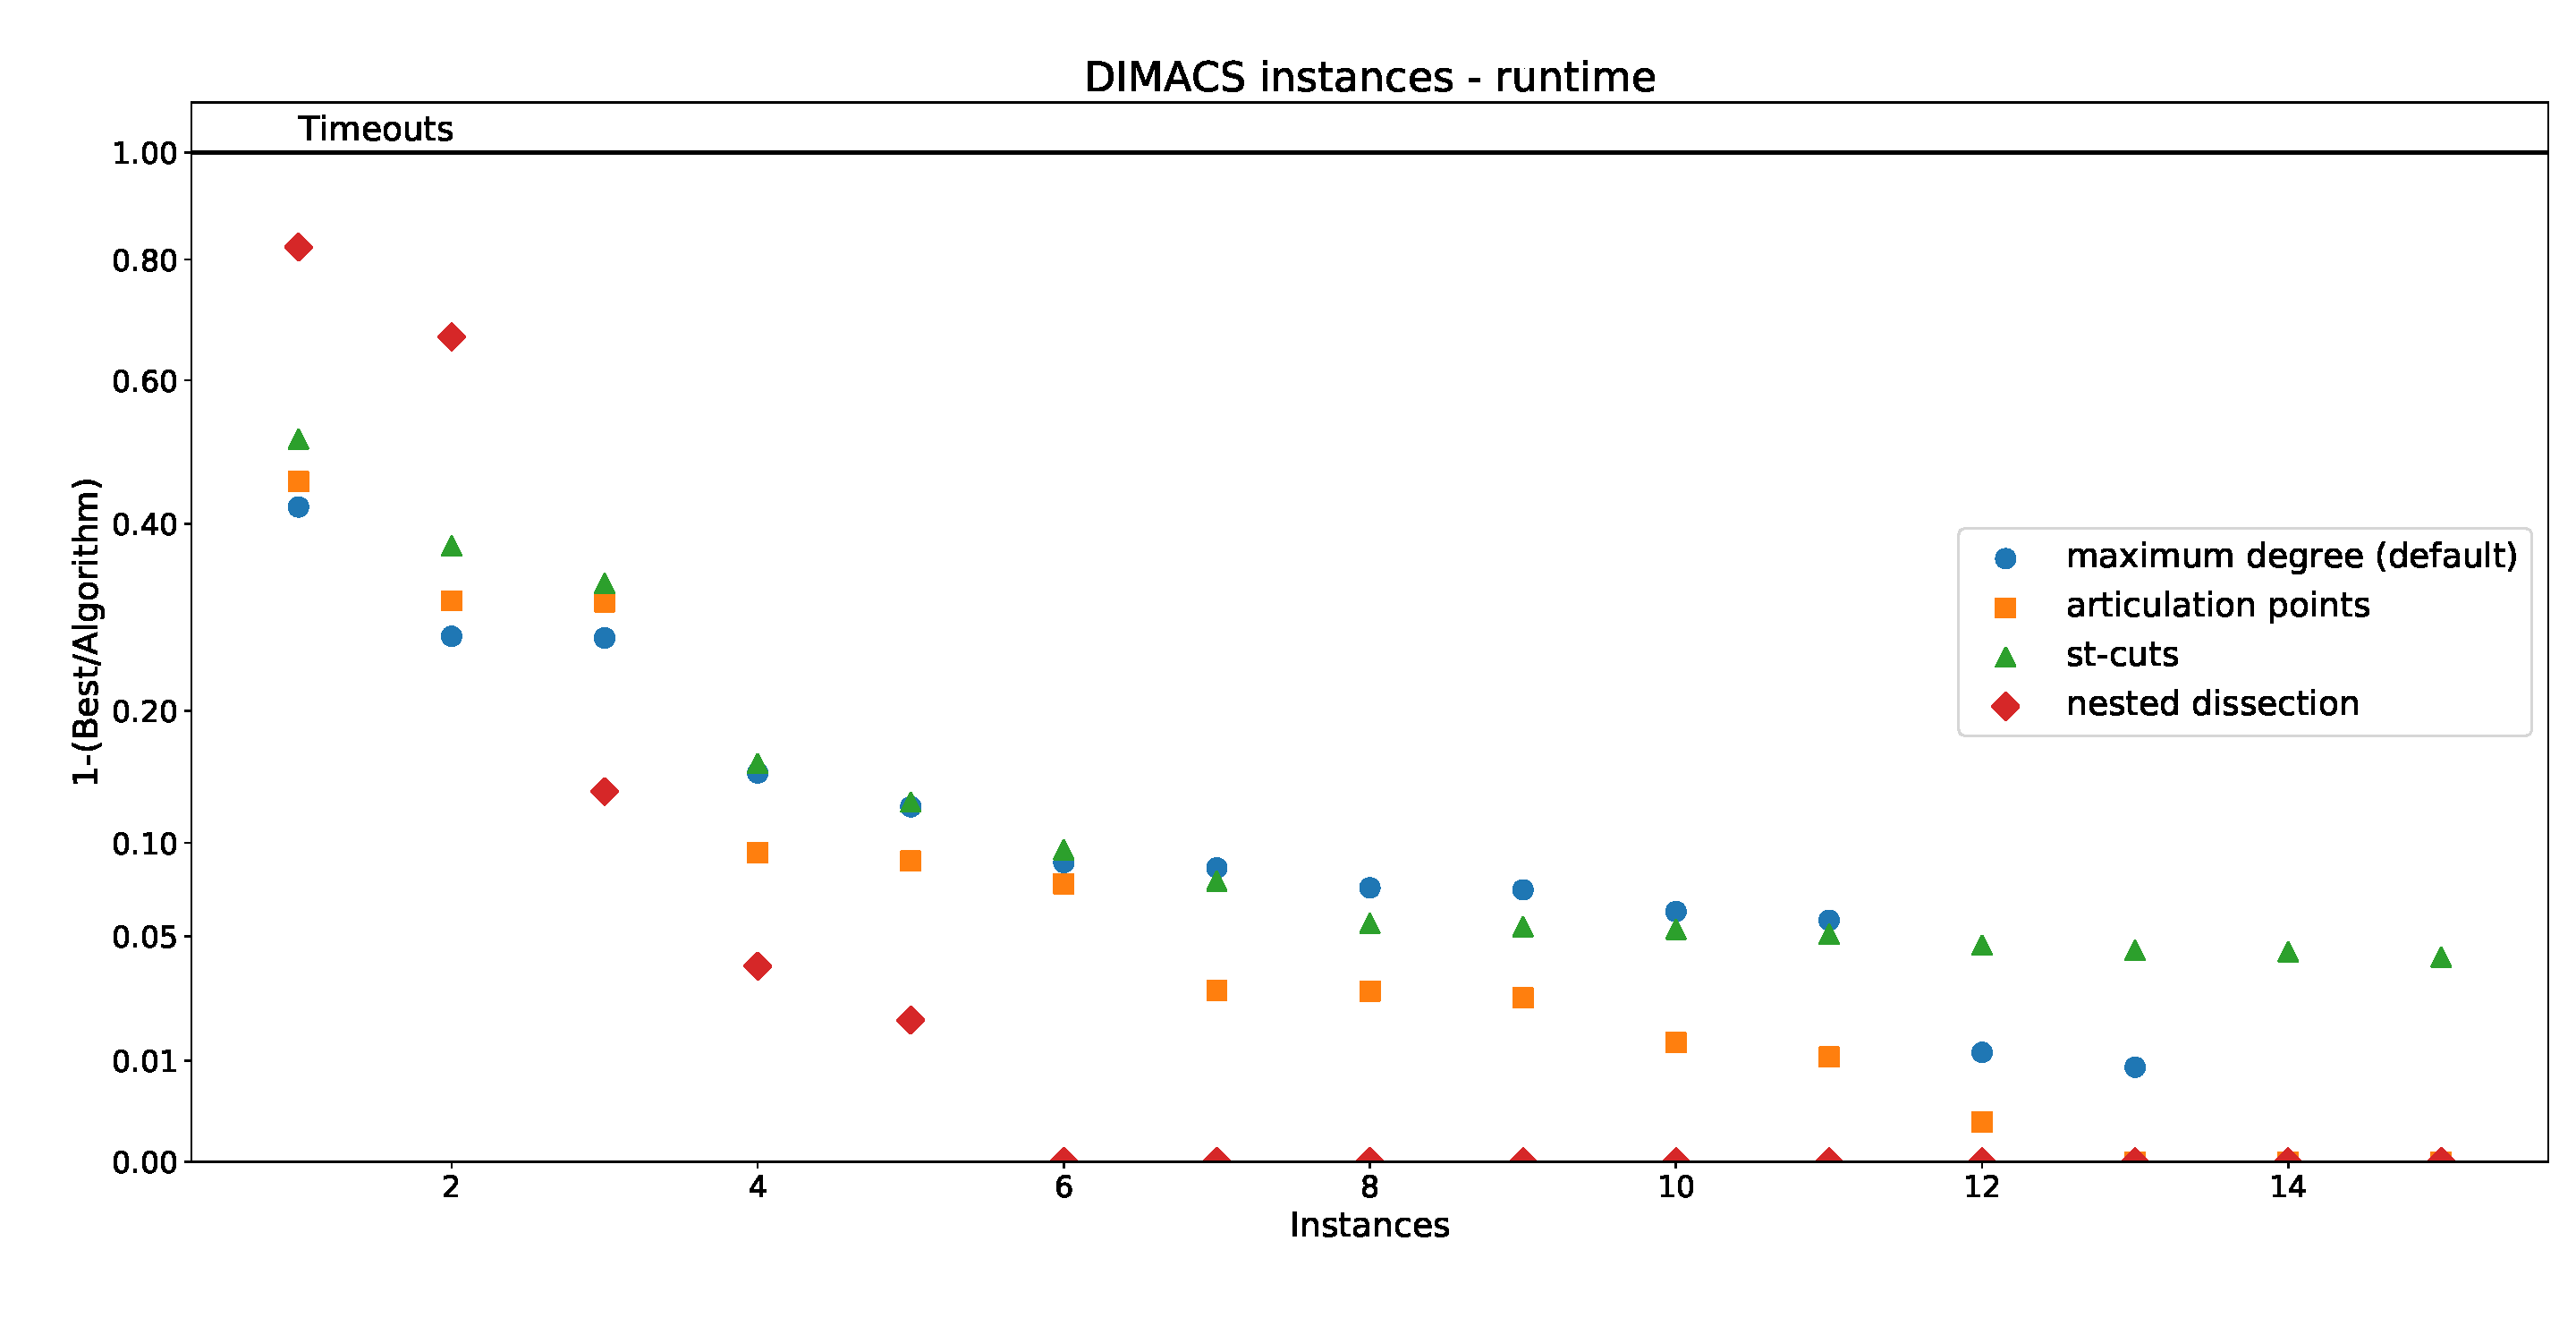
\includegraphics[width=\textwidth]{images/plots/a1_dimacs_t}
		\caption{runtime}
	\end{subfigure}
	\begin{subfigure}{1\textwidth}
		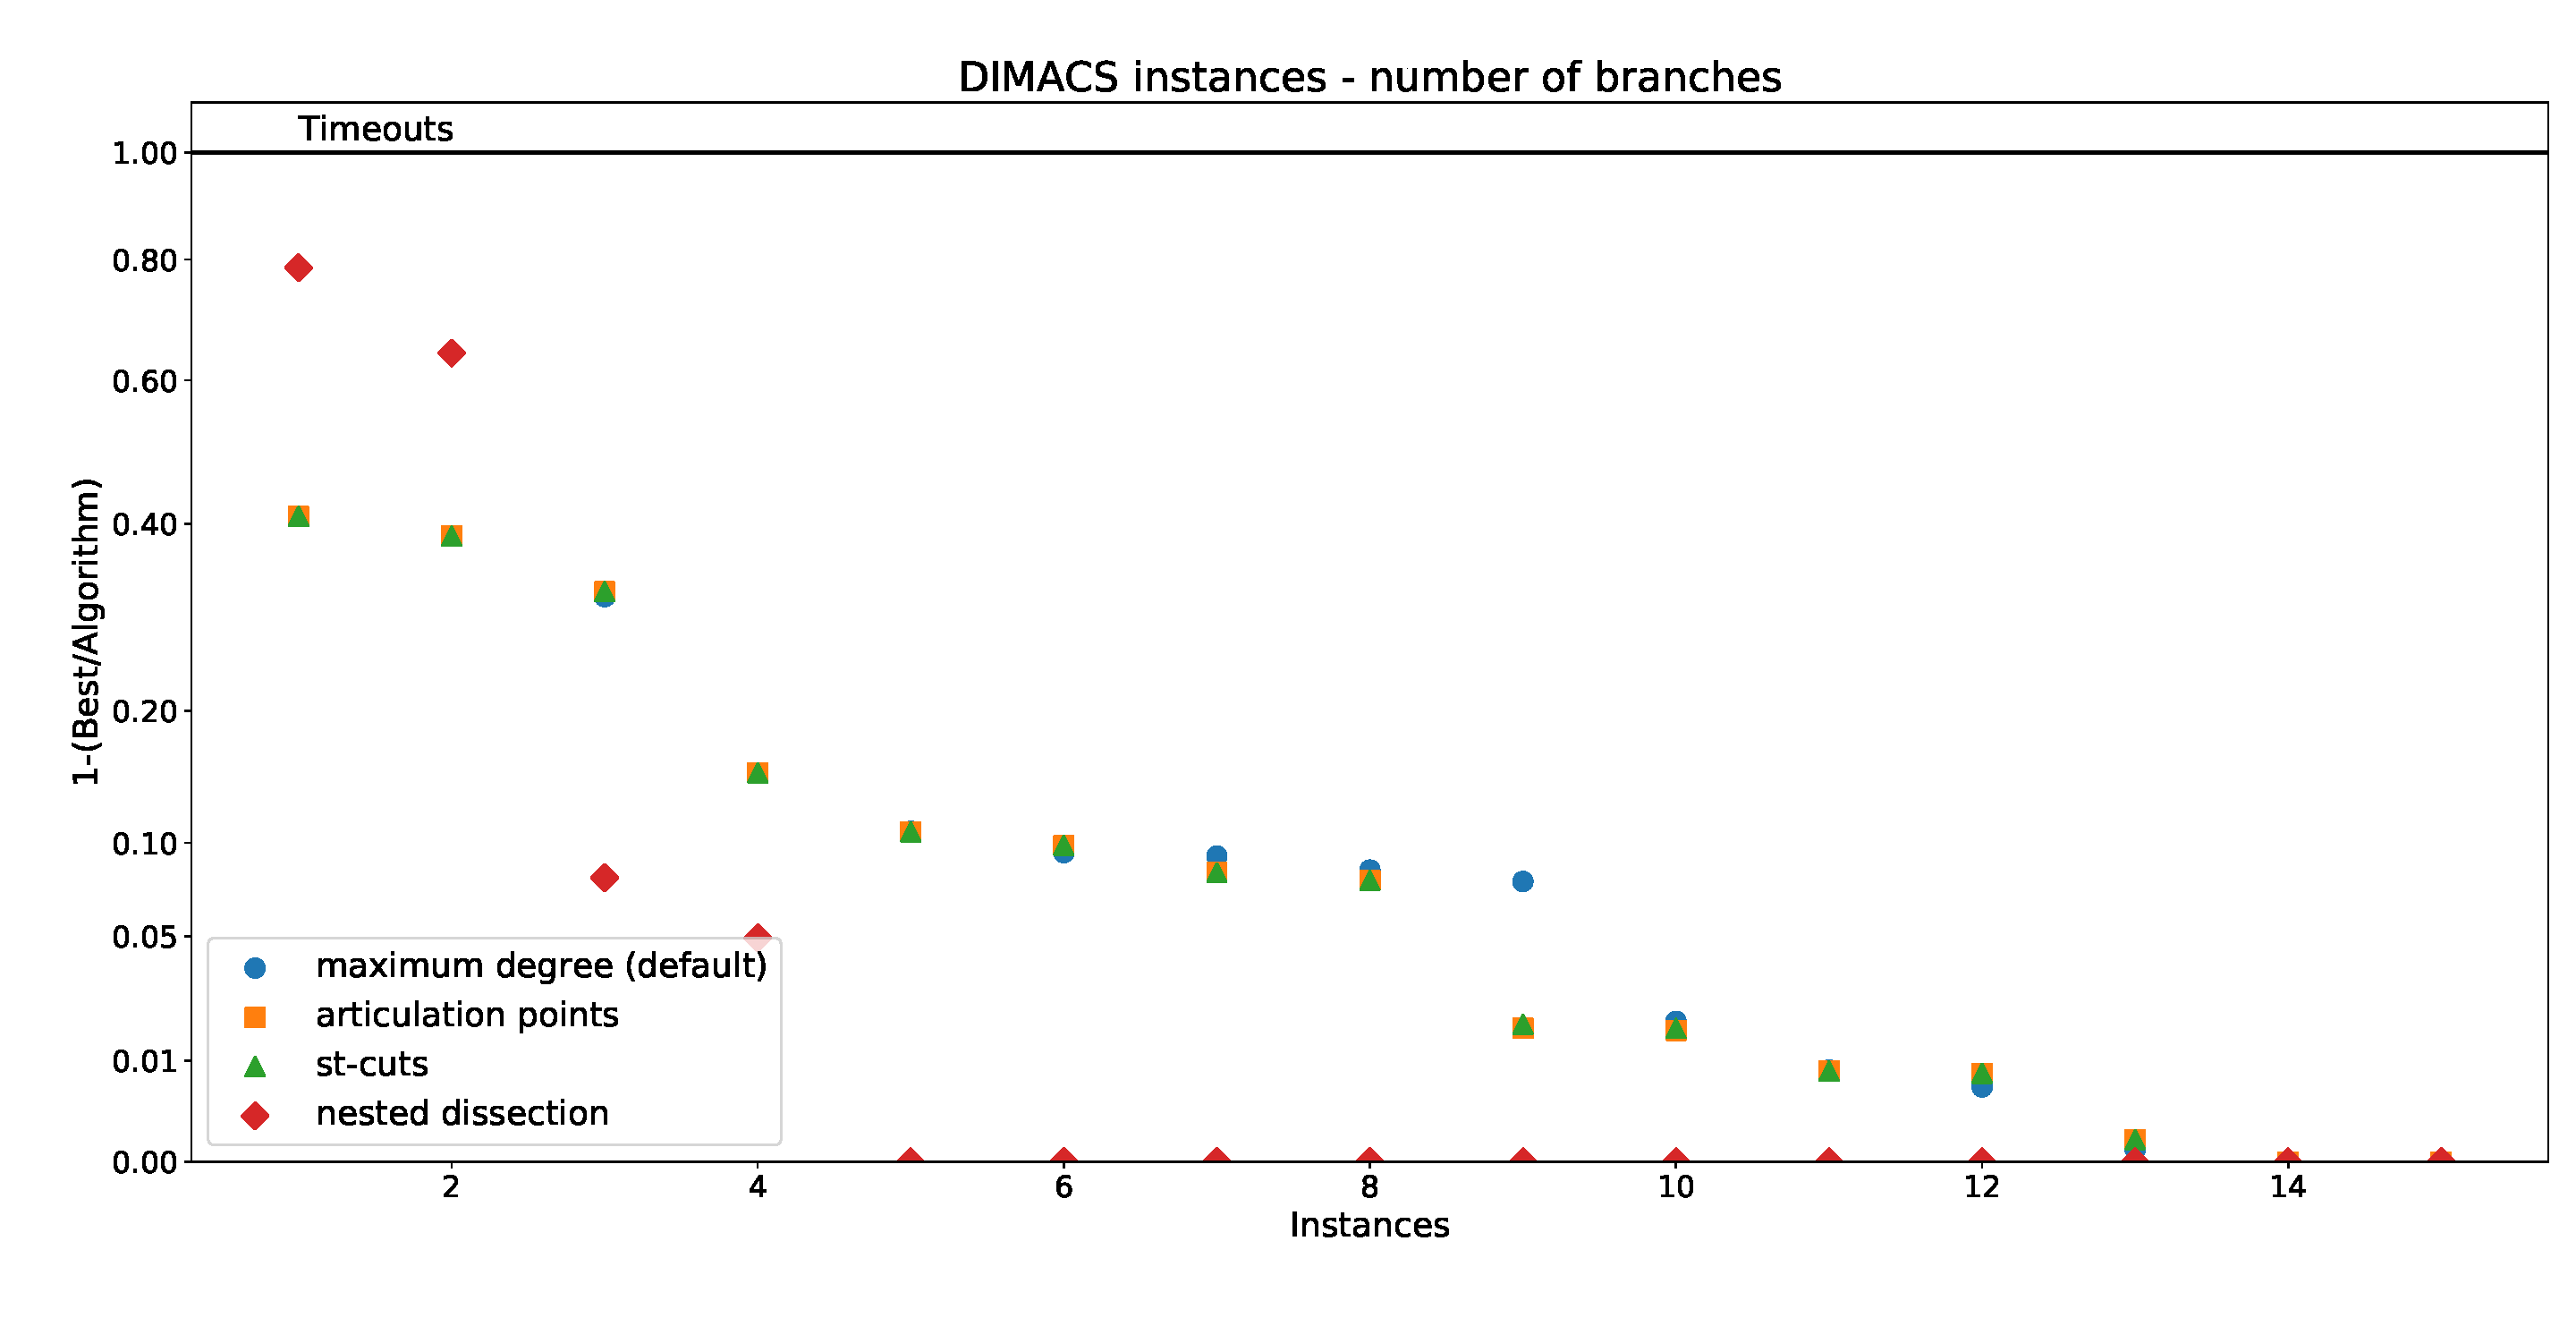
\includegraphics[width=\textwidth]{images/plots/a1_dimacs_b}
		\caption{number of branches}
	\end{subfigure}
	\caption{Performance plots of decomposing branching strategies on DIMACS instances}
\end{figure}
\begin{figure}[hbt!]
	\begin{subfigure}{1\textwidth}
		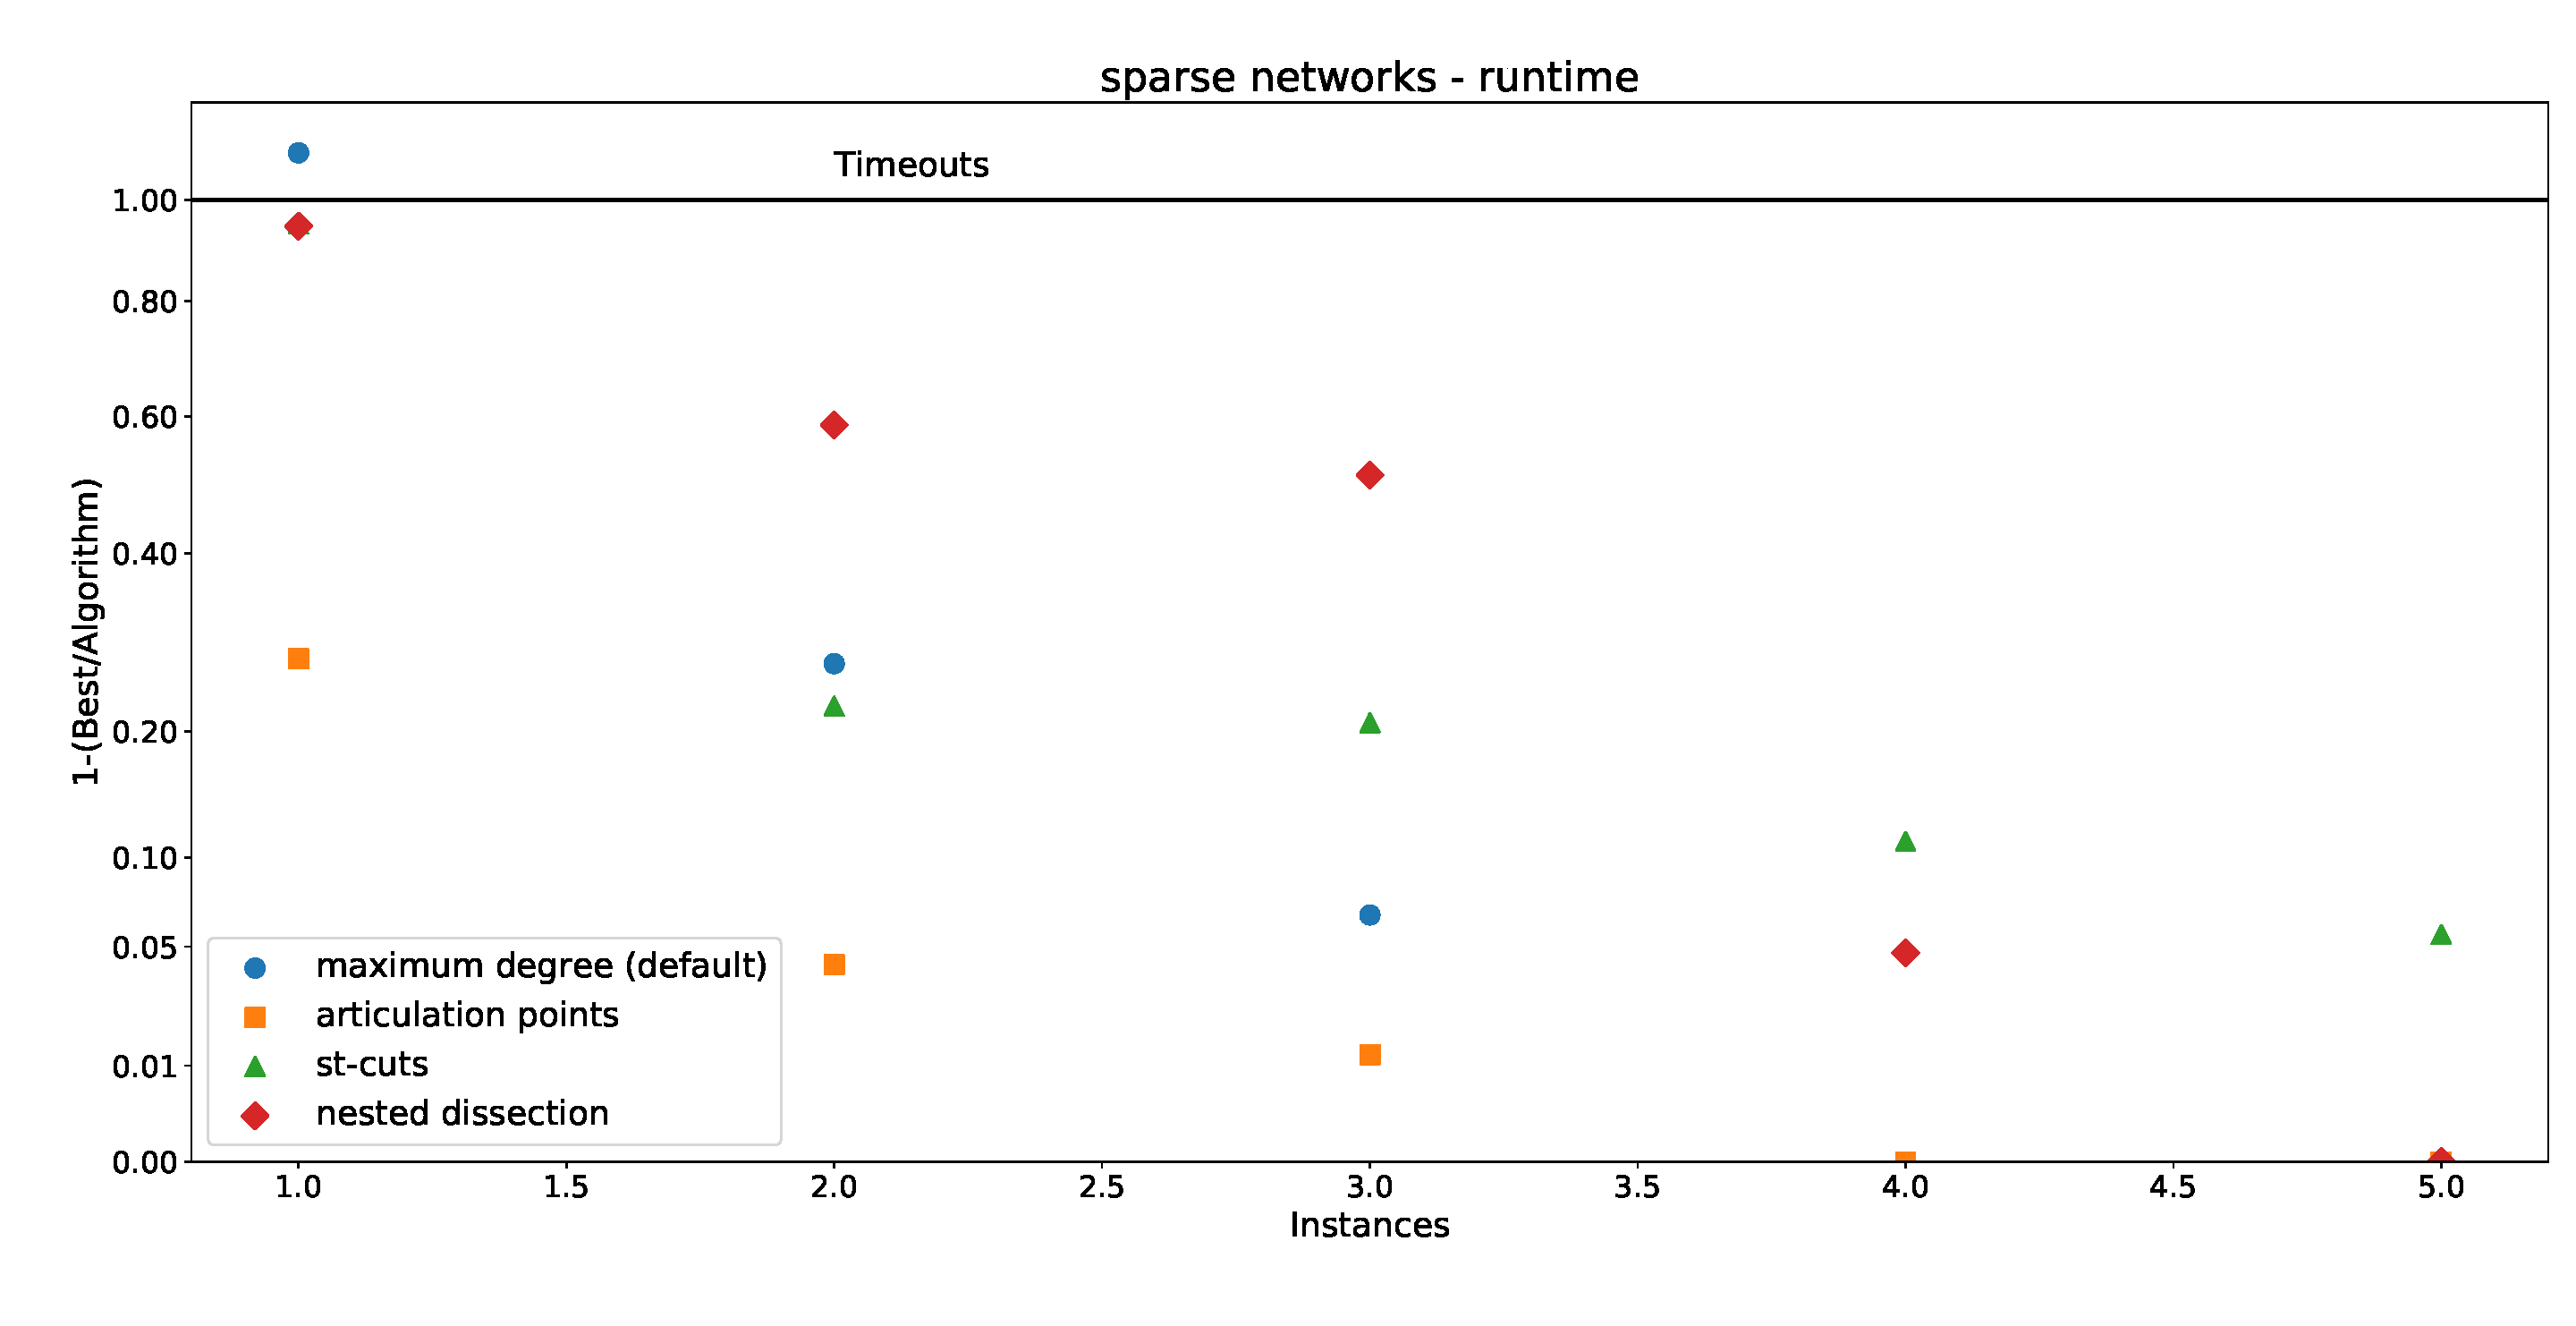
\includegraphics[width=\textwidth]{images/plots/a1_sn_t}
		\caption{runtime}
	\end{subfigure}
	\begin{subfigure}{1\textwidth}
		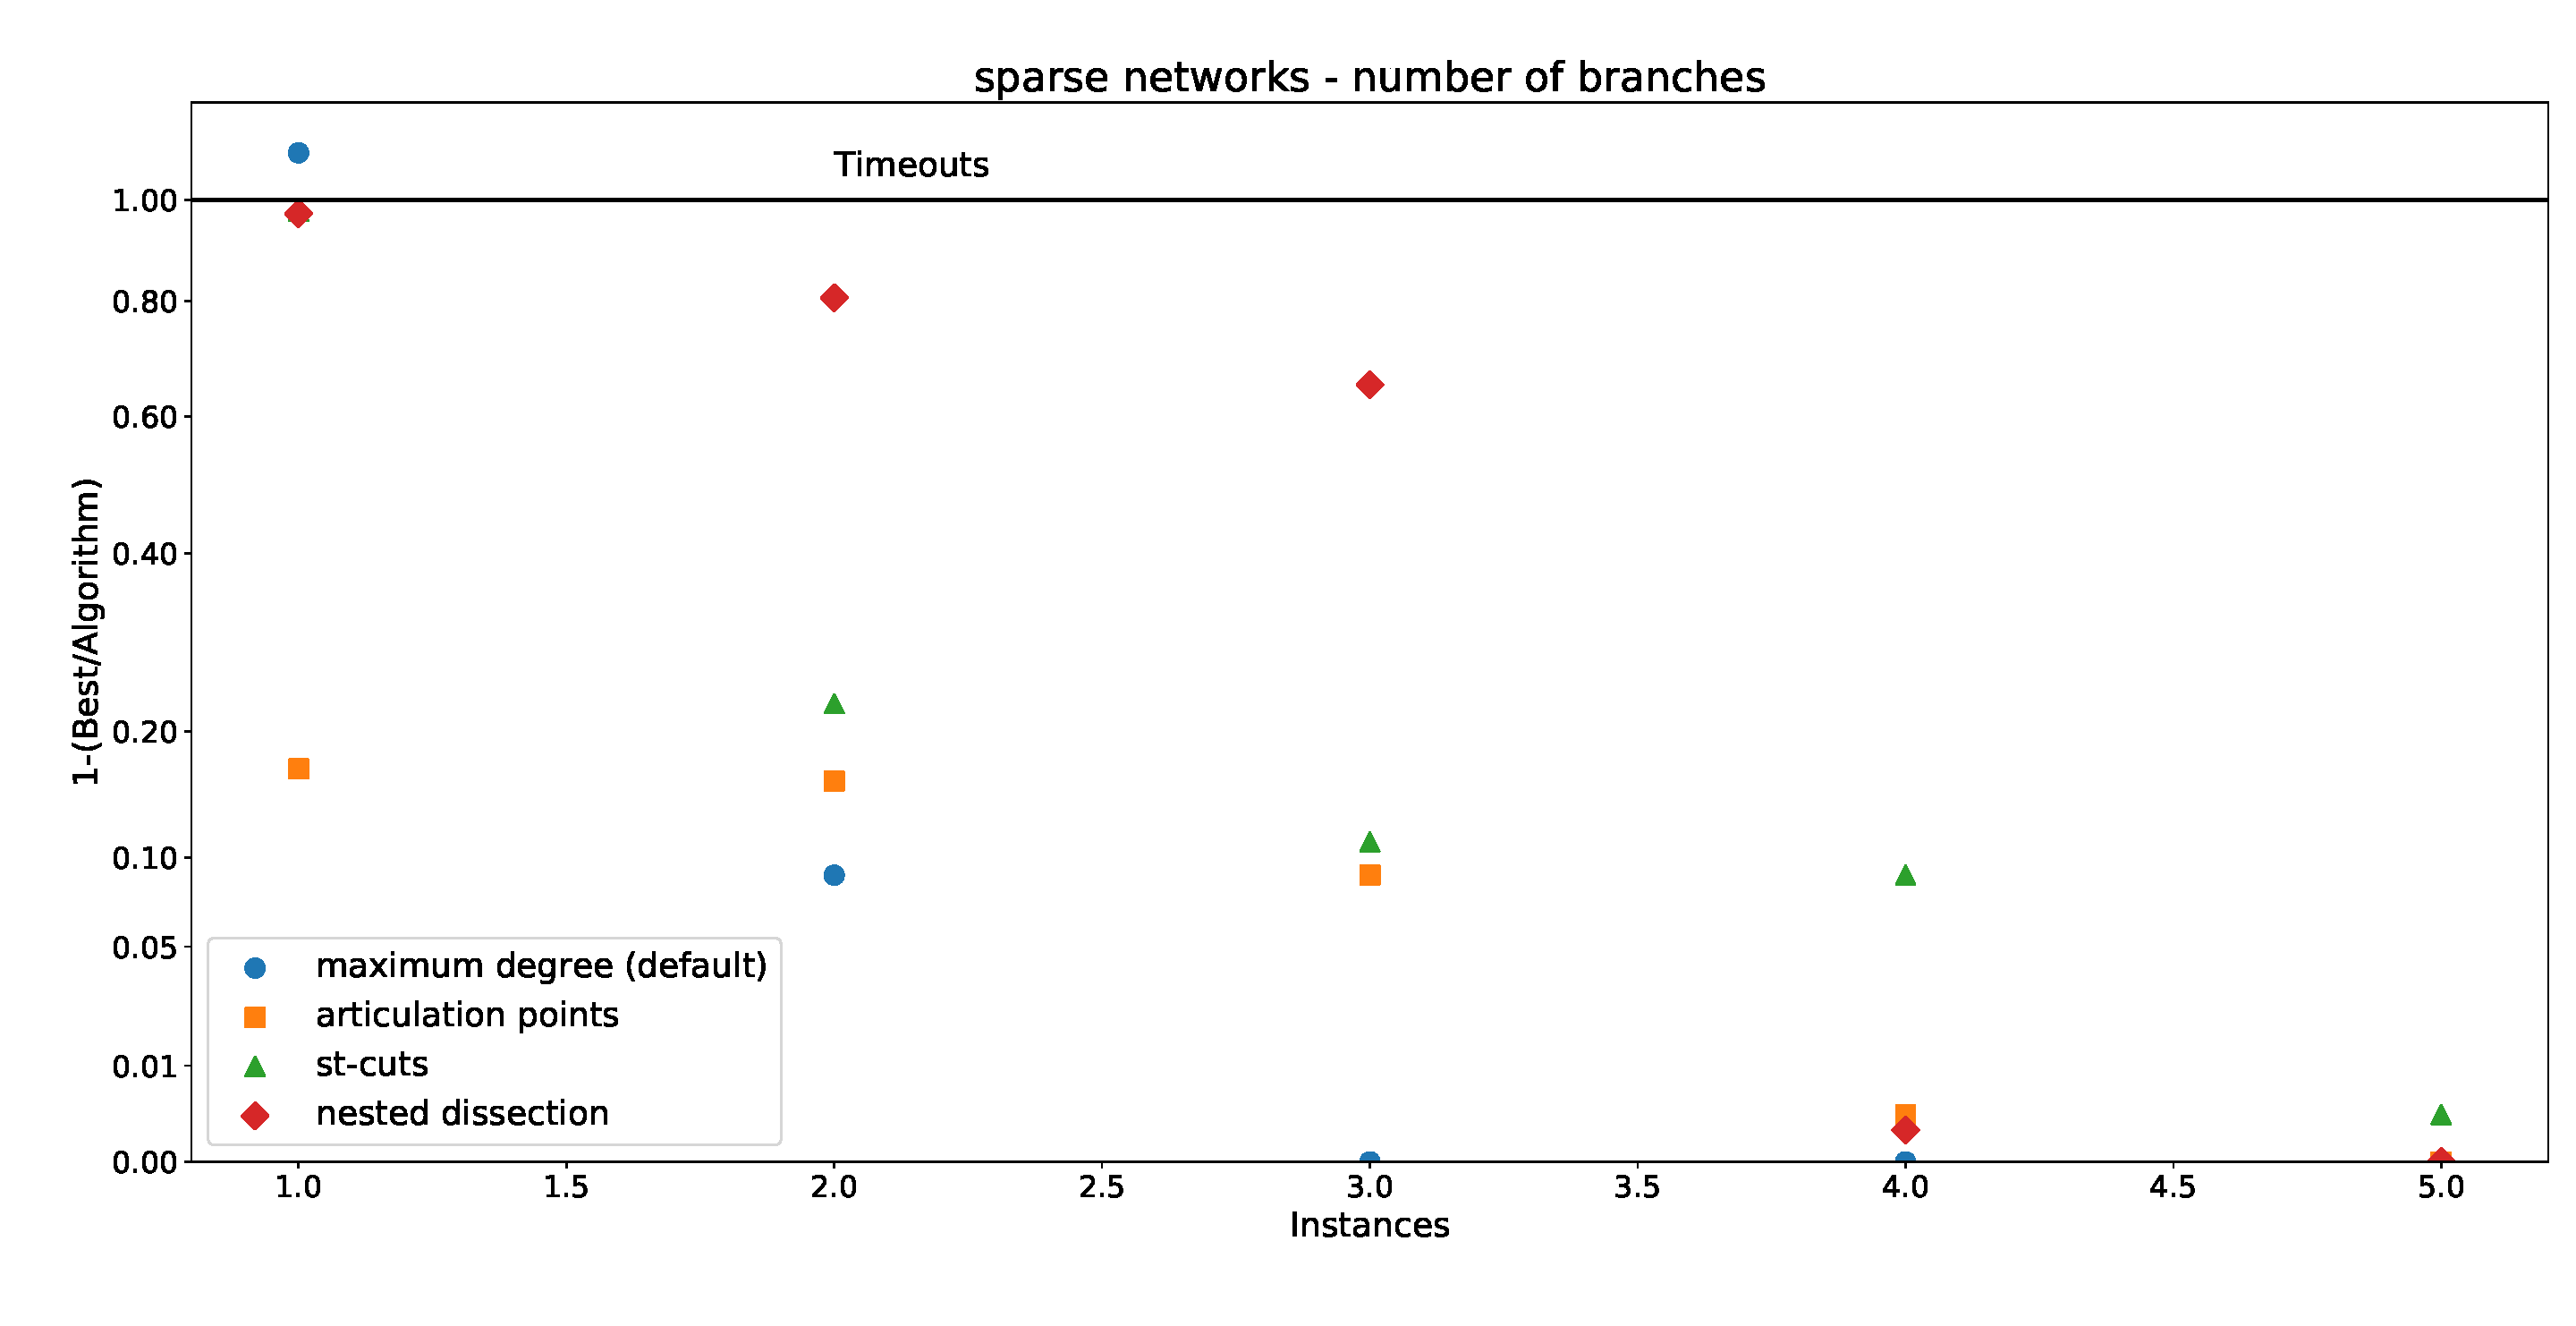
\includegraphics[width=\textwidth]{images/plots/a1_sn_b}
		\caption{number of branches}
	\end{subfigure}
	\caption{Performance plots of decomposing branching strategies on sparse networks}
\end{figure}

\begin{figure}[hbt!]
	\begin{subfigure}{1\textwidth}
		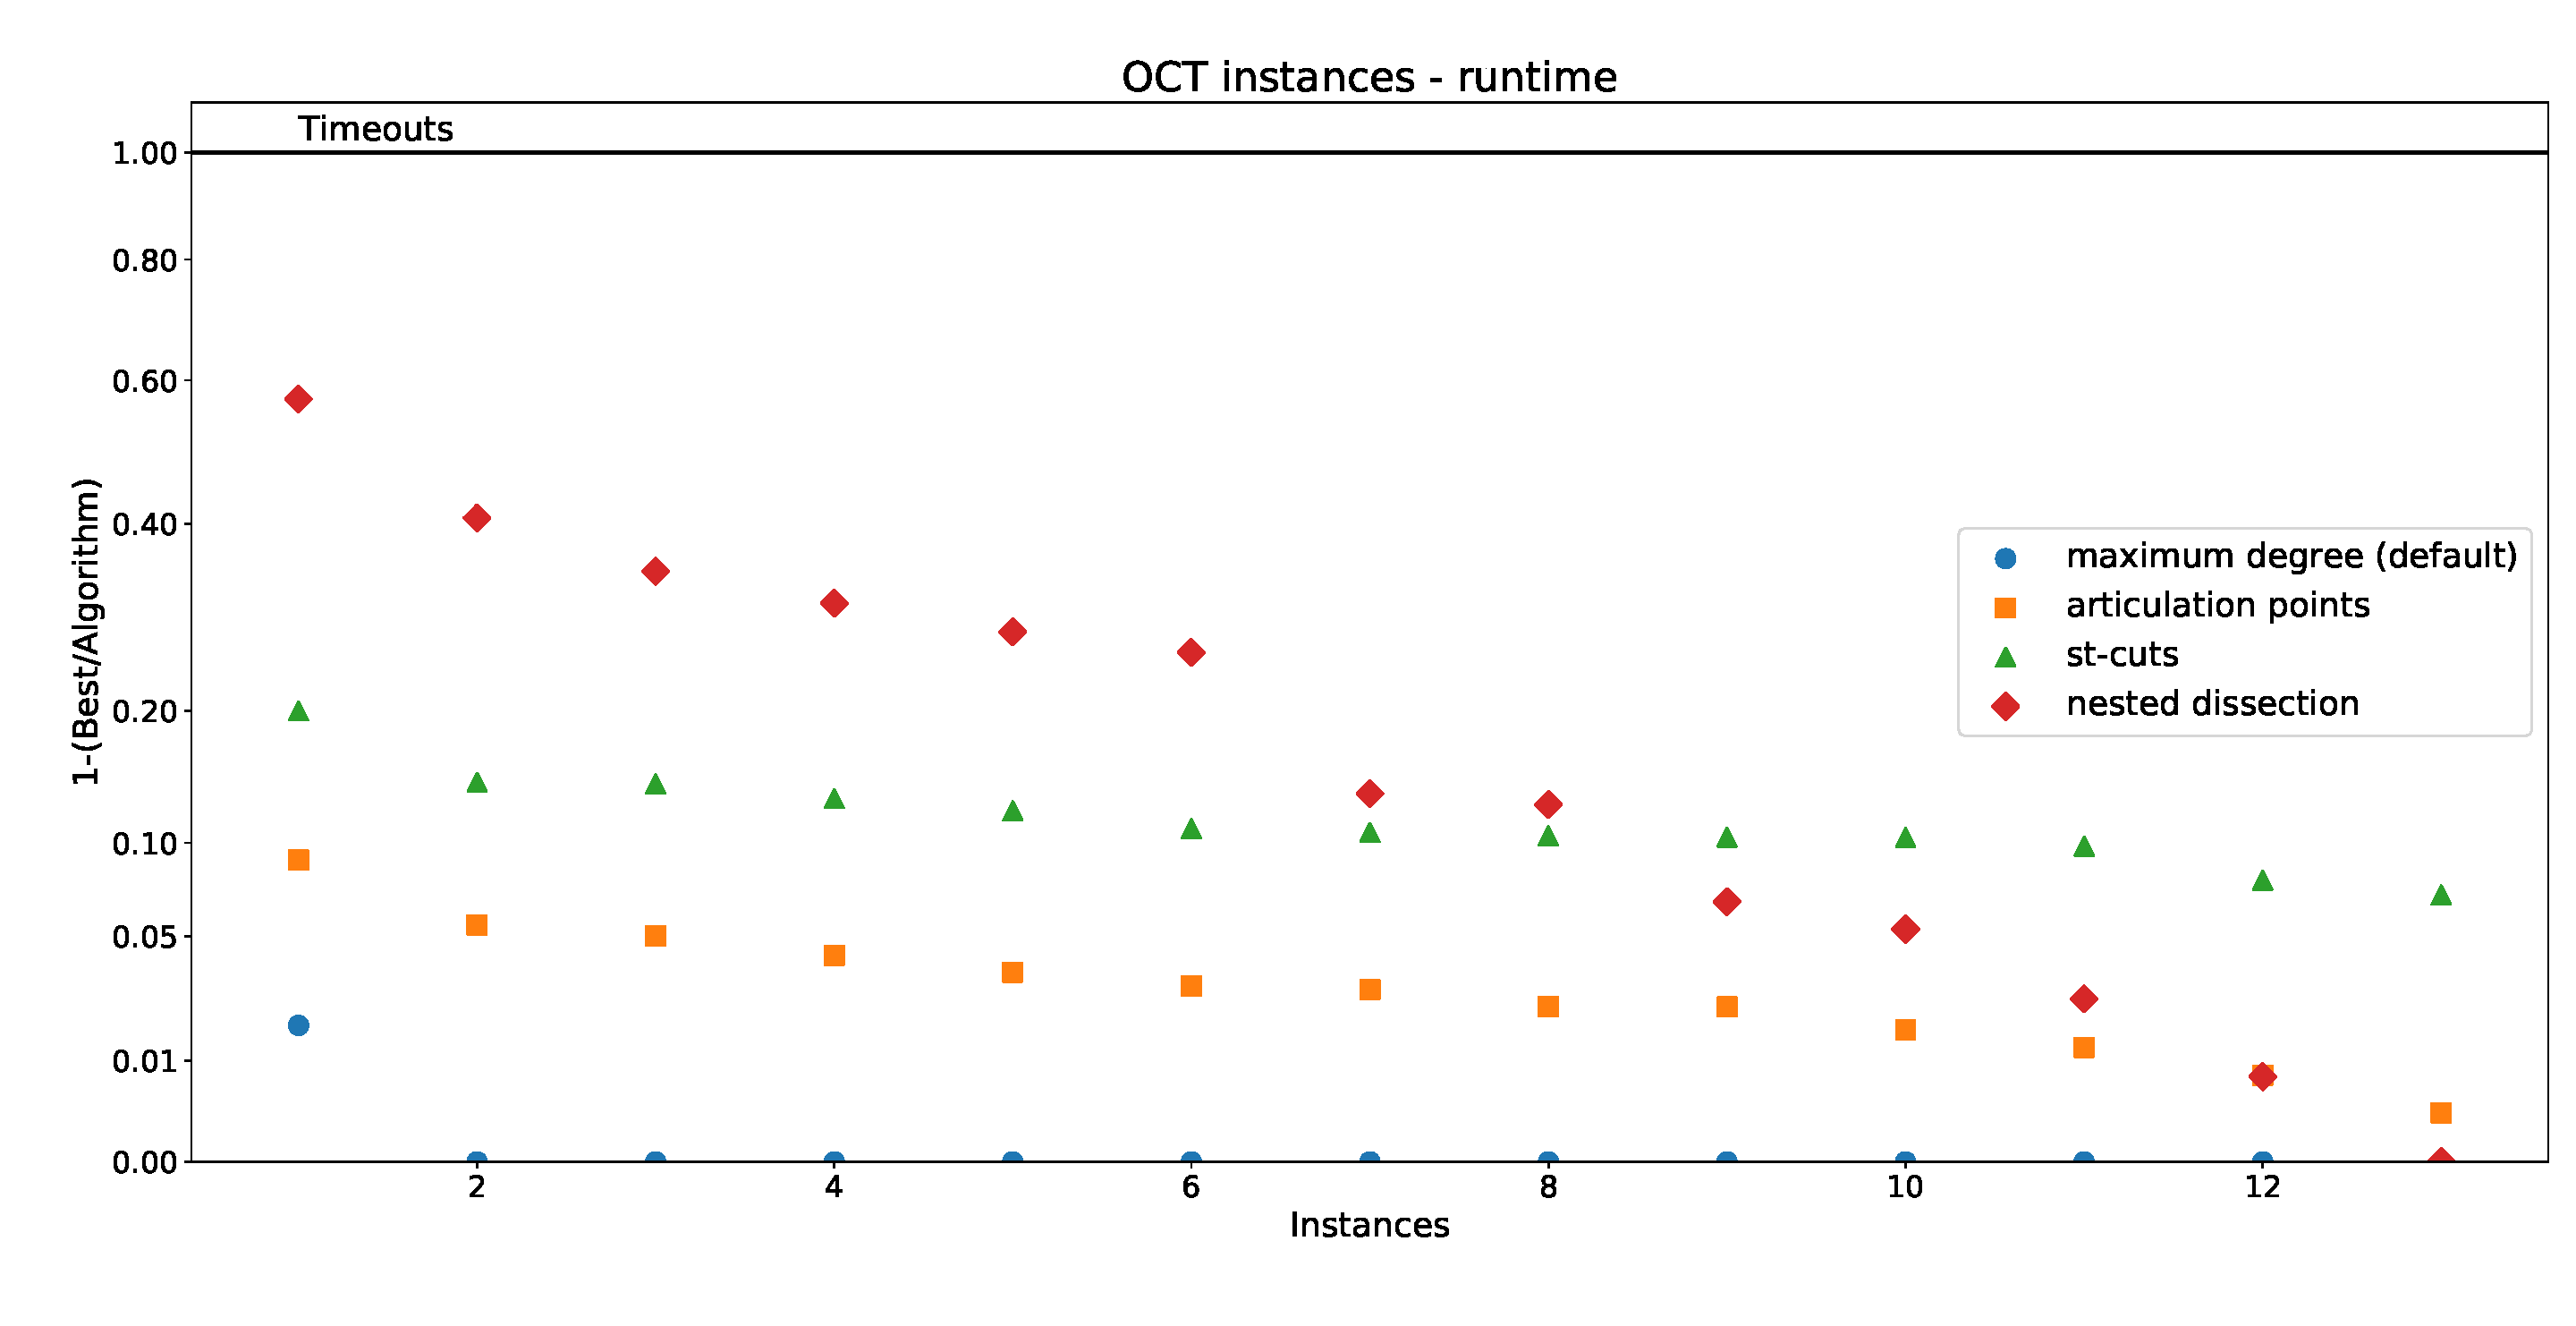
\includegraphics[width=\textwidth]{images/plots/a1_oct_t}
		\caption{runtime}
	\end{subfigure}
	\begin{subfigure}{1\textwidth}
		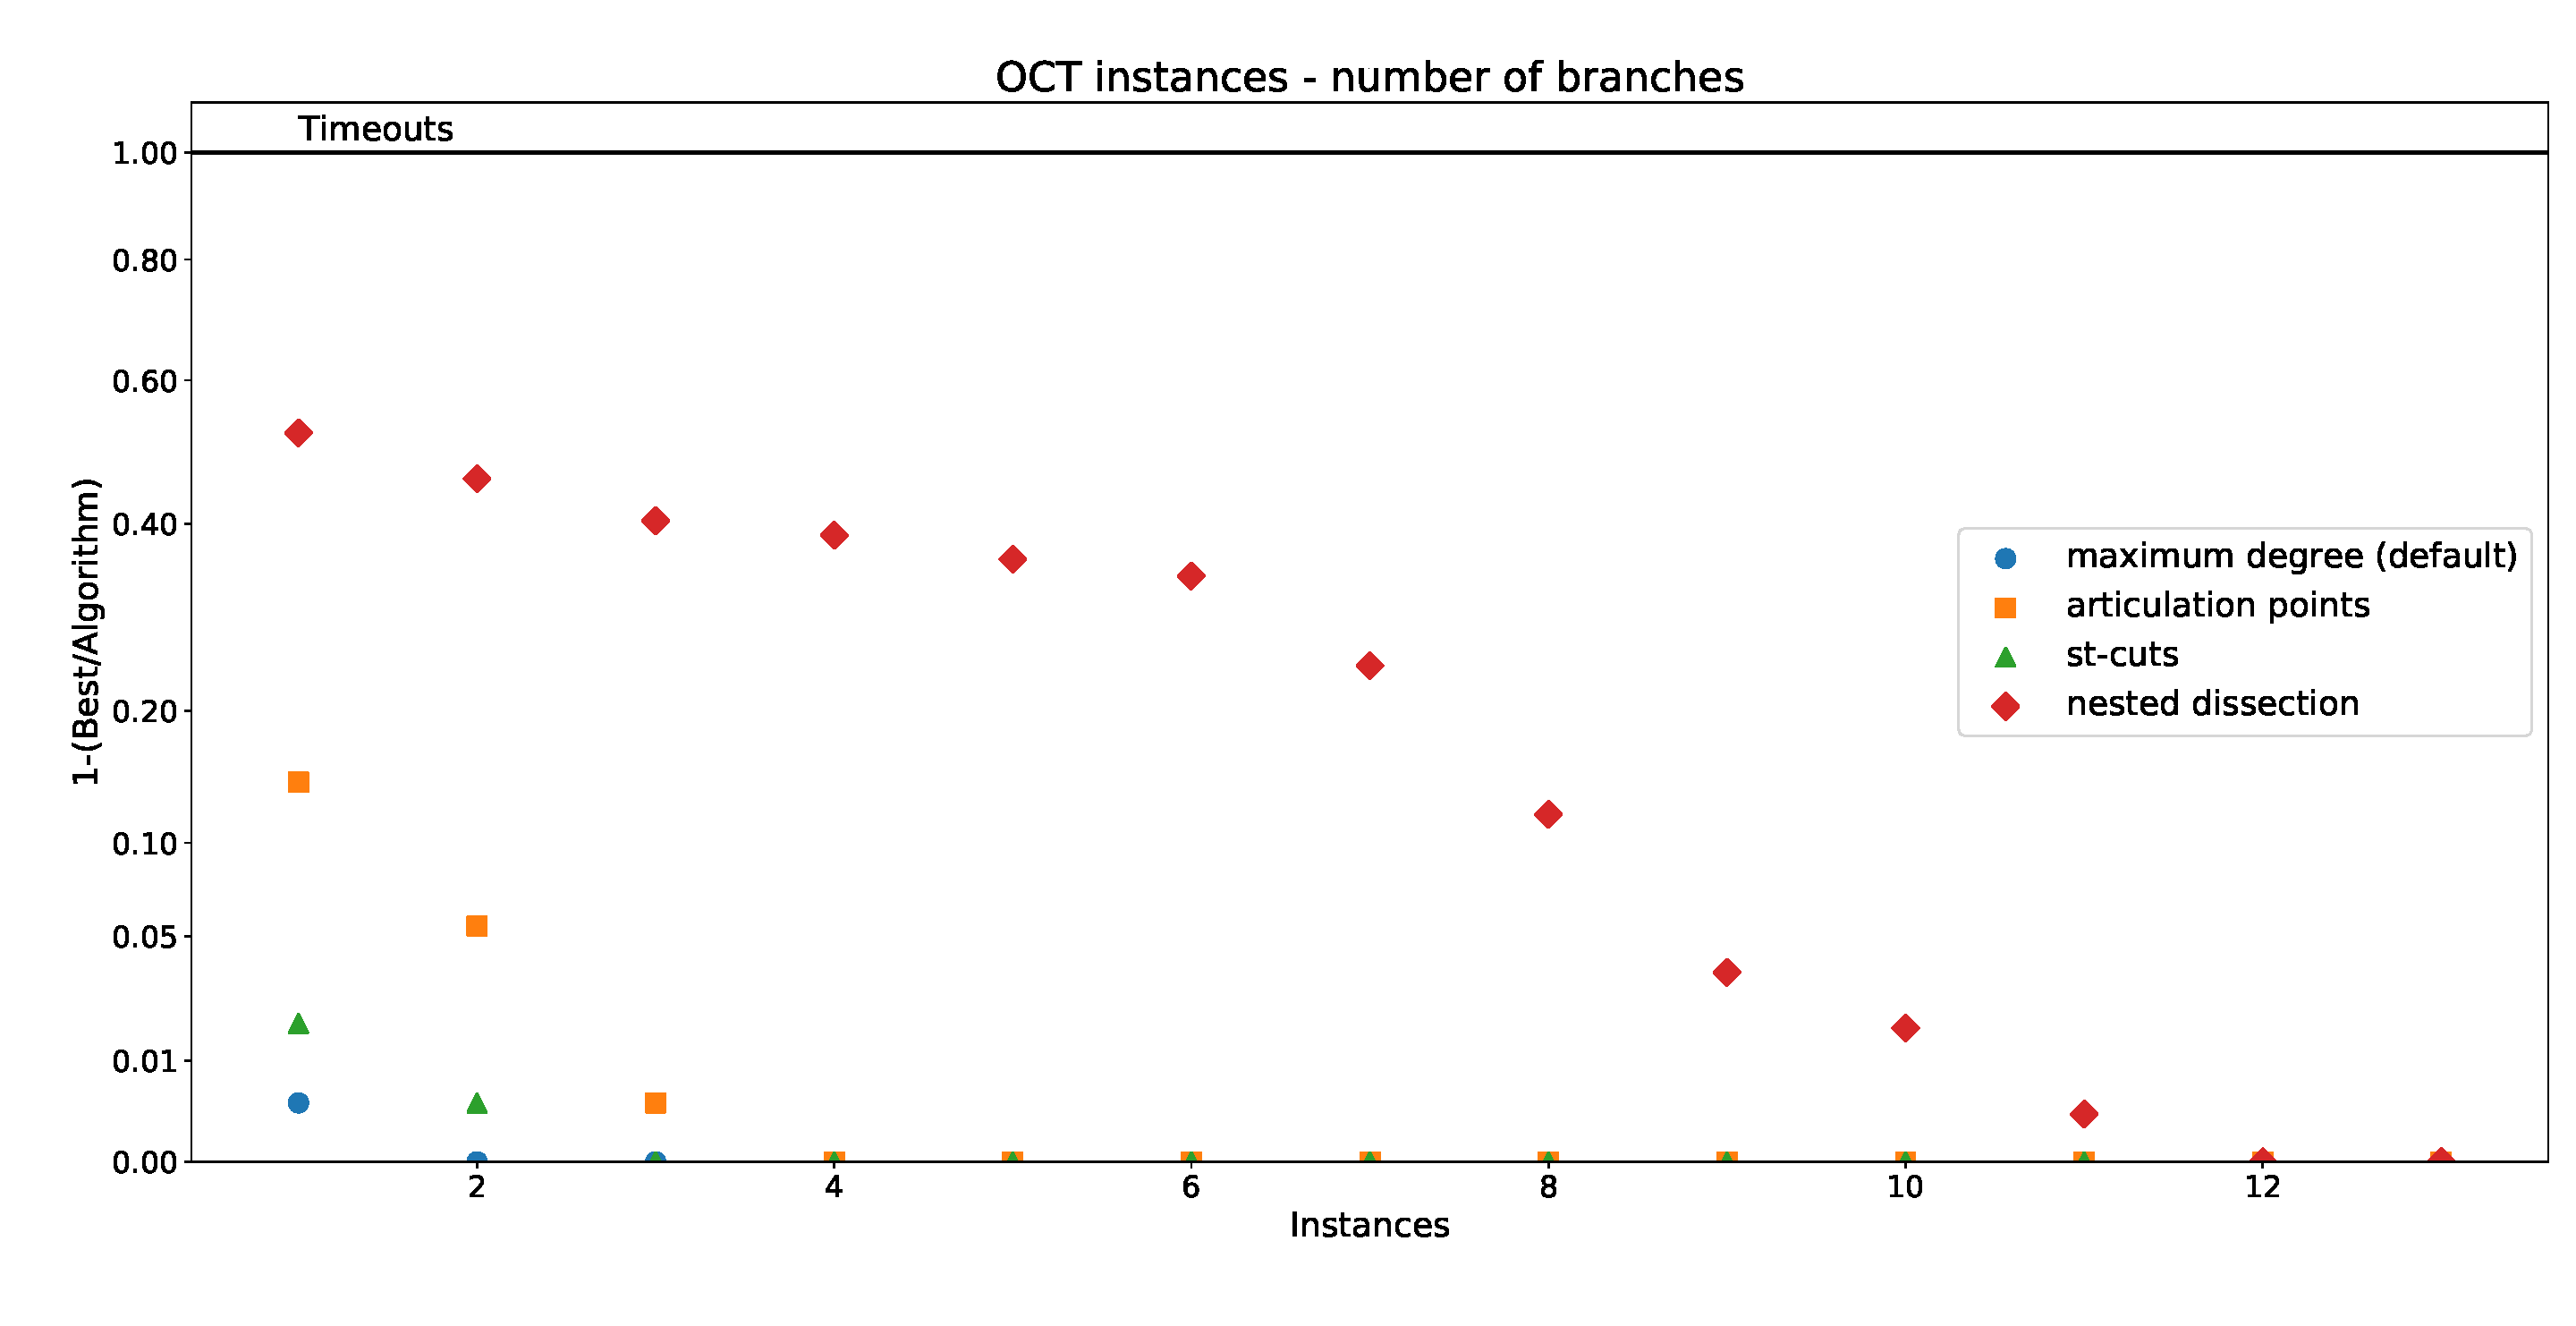
\includegraphics[width=\textwidth]{images/plots/a1_oct_b}
		\caption{number of branches}
	\end{subfigure}
	\caption{Performance plots of decomposing branching strategies on graphs obtained from OCT instances}
\end{figure}

\begin{figure}[hbt!]
	\begin{subfigure}{1\textwidth}
		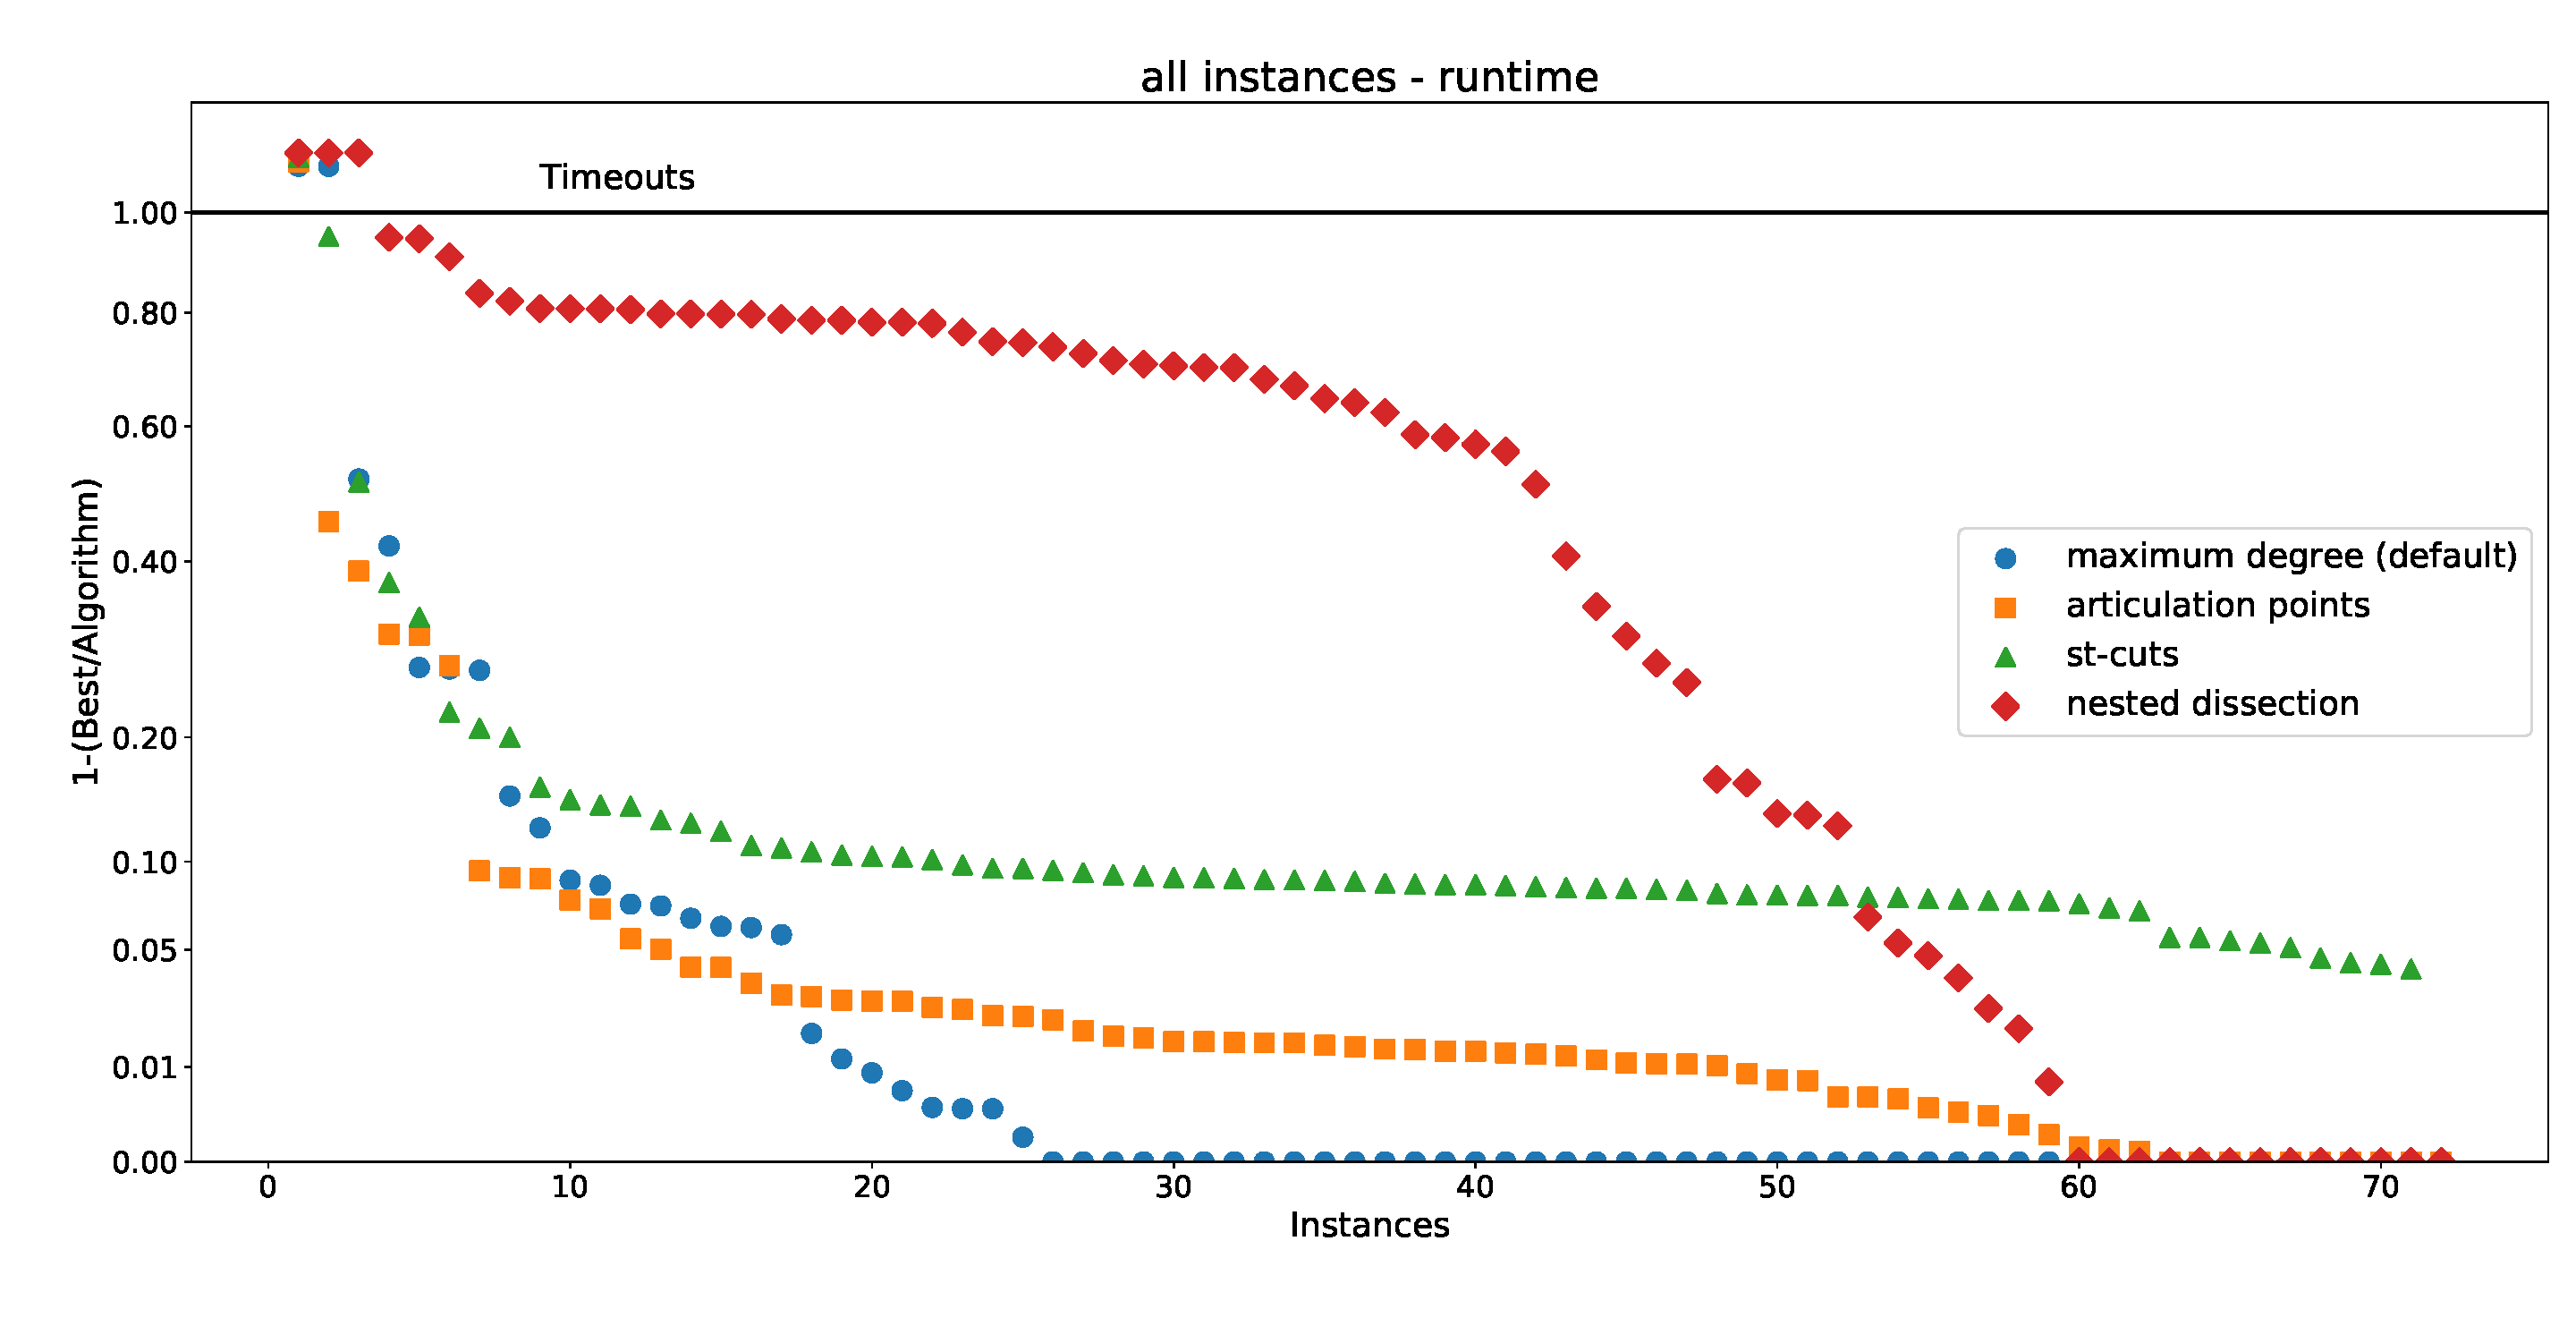
\includegraphics[width=\textwidth]{images/plots/a1_all_t}
		\caption{runtime}
	\end{subfigure}
	\begin{subfigure}{1\textwidth}
		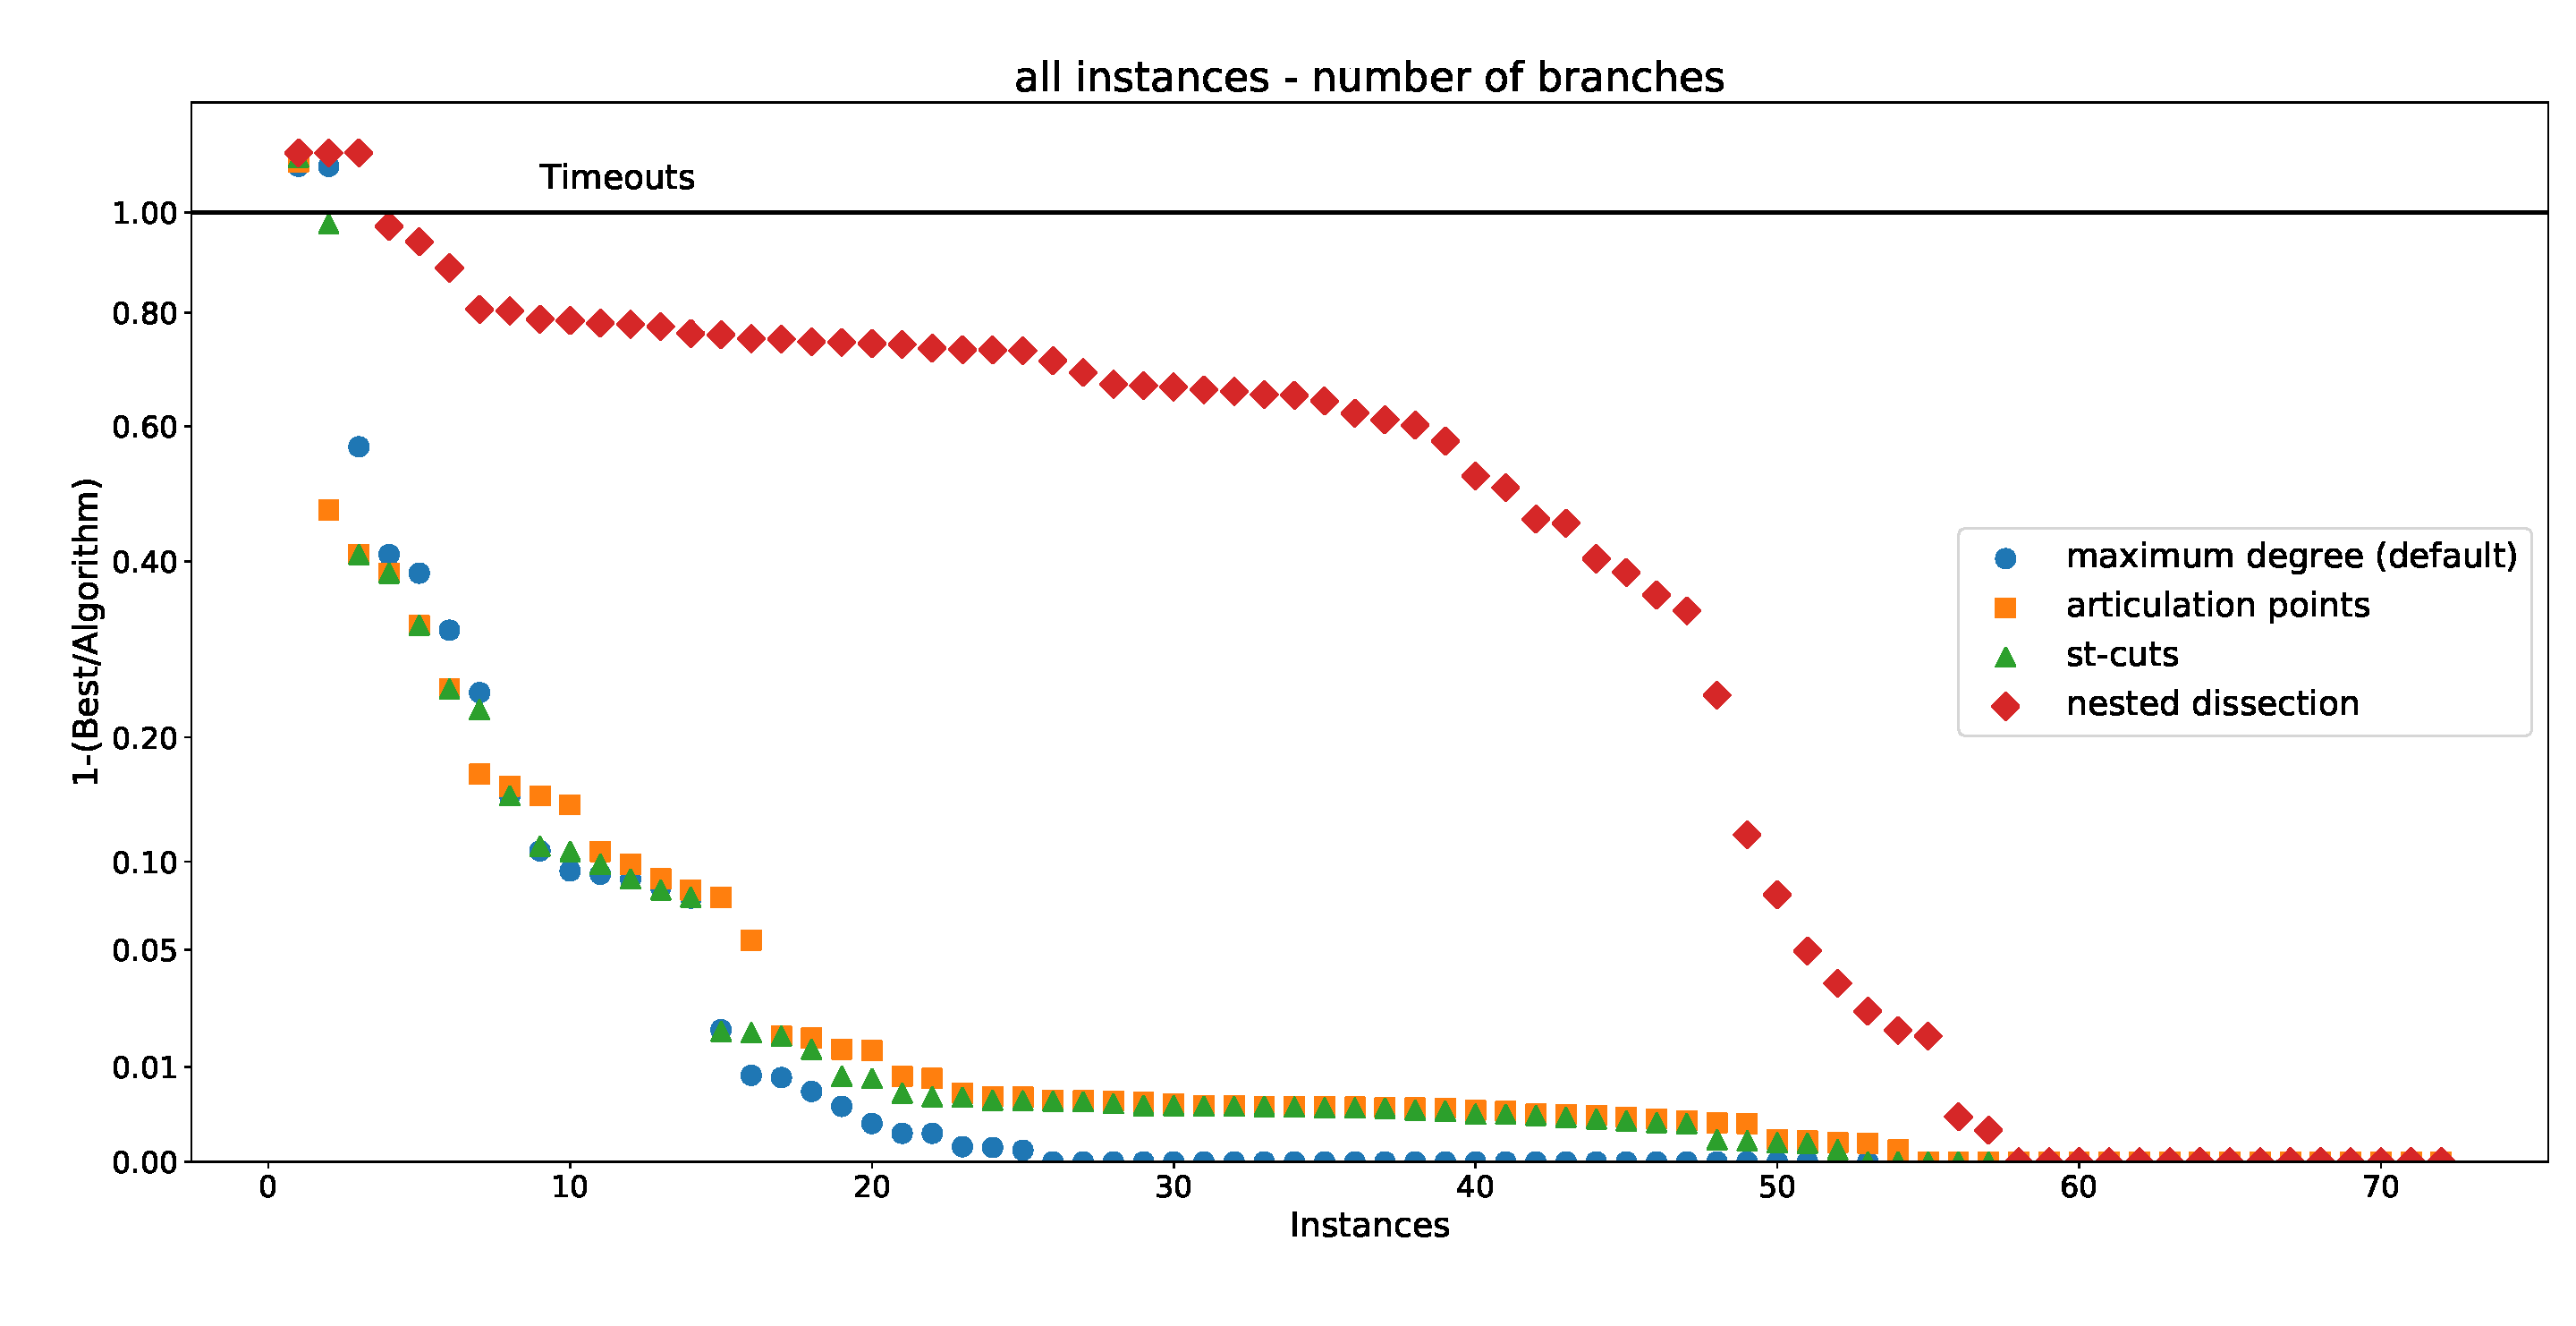
\includegraphics[width=\textwidth]{images/plots/a1_all_b}
		\caption{number of branches}
	\end{subfigure}
	\caption{Performance plots of decomposing branching strategies on all instances}
	\label{22}
\end{figure}
\clearpage

\subsubsection{Evaluation of Branching Strategies Based on Reduction Rules}
Next, we compare the branching strategies following our second approach which is to branch on vertices so that reduction rules become applicable afterwards. The experimental results are depicted in Figures \ref{111} to \ref{222}. Unfortunately, due to the restricted scope of this thesis, we have only implement a preliminary version of our branching strategy targeting reduction chains. This implementation performs considerably worse than default branching on all instances. For the sake of clarity, we omitted these results in our plots.

\paragraph{}
Using the branching strategy based on dominance reduction almost always reduces the total number of branching steps needed for solving PACE and DIMACS instances to a minor extent, i.e., less than two percent on average. Unfortunately, dominance reduction is not applied in the branch and reduce algorithm, since it is fully contained in the unconfined reduction. Therefore, finding suitable vertices that enable the application of dominance reduction upon removal comes with additional time overhead of up to five percent of the total runtime. 

\paragraph{}
The branching strategy based on unconfined reduction reduces the total number of branching on PACE instances by a similar amount than the strategy based on dominance reduction. However, vertices considered for branching can be found during kernelization while searching unconfined vertices. Nevertheless, this still produces a non negligible time overhead. On PACE instances this strategy performs roughly equal to the branching strategy based on dominance reduction. It is about three percent slower on average than the default branching strategy. On seven of the DIMACS instances, however, this strategy performs up to ten percent better than default branching and is at most five percent slower on the other DIMACS instances. Considering all DIMACS instances this branching strategy is about two percent faster than default branching.
\paragraph{}
In total, the branching strategies utilizing dominance and unconfined reduction perform worse than the default branching strategy on PACE instances. On DIMACS instances the latter strategy has a small advantage over default branching.
\paragraph{}
On sparse networks both strategies perform better than default branching on two of the instances. A reason for this may be that the average vertex degree on those graphs is much lower than on denser graphs. Moreover, vertices with high degree are quickly removed by branching at an early stage of the algorithm. Thus, verifying whether a vertex is almost dominated or almost unconfined is much faster in relation to overall kernelization time since fewer adjacencies have to be checked.

\paragraph{}
The branching strategy based on the twin reduction rule overall performs slightly better than the default strategy on PACE and DIMACS instances. However, the speedup is only about two percent on average considering all PACE and DIMACS instances. This is due to the fact that on those graphs almost twins are rarely found. Nevertheless, finding vertices that enable twin reduction produces very little overhead. Also, applying twin reduction is very efficient, since the number of vertices in the graph is reduced by four to five. For those reasons, this branching strategy has an advantage over default branching on four of the five sparse networks tested. Using this branching strategy reduces the running time by up to twelve percent. Since the average degree on those graphs is very low, vertices considered for branching are found more often. On OCT instances the performance of this branching strategy is roughly equal to default branching.
\paragraph{}
Our last branching strategy targeting the funnel reduction overall requires the least number of branching steps, i.e., about ten percent less on average, to solve PACE instances. There are only two PACE instances where the strategy based on unconfined reduction requires less branching steps. Except on these two instances this strategy also reduces the required runtime compared to default branching by about five percent on average. Also, on seven of the DIMACS instances, this branching strategy performs best in terms of total number of branching steps needed. However, the reduction in branching steps does not compensate for the time overhead caused by finding almost funnels on all of theses instances. Overall, this strategy performs worse than the default branching strategy on DIMACS instances with runtimes which are two percent higher on average. On sparse networks this branching strategy also seems to be competitive to default branching. On two instances it requires the least number of branching steps. Considering the runtime it is, however, worse than default branching on all but two instance. In total, it is about three percent slower than default branching. Furthermore, it is outperformed by the strategy based on twin reduction on every instance. A possible explanation for this is that funnel reduction removes the common neighbors of both parts of the funnel. On denser graphs the common neighborhood of a funnel is potentially larger. Thus, funnel reduction is more effective on those graphs than on sparse networks.

\paragraph{}
The experiments using branching strategies following our second approach demonstrate that branching in order to enable reduction rules can effectively reduce the total number of branches needed to solve an instance. Contrary to our first approach, this also works on denser graphs. These branching strategies also yield more constant results with fewer outliers. Unfortunately, the reduction in branching steps does not always compensate for the additional overhead caused by finding suitable branching vertices. Overall, targeting funnel and twin reduction worked very well where as targeting dominance and unconfined reductions do not improve the algorithms runtime in most cases. A reason for this might be that, as shown by Stallmann et al. \cite{Stallmann}, dominance and unconfined reduction are also applied often on dense graph using the default branching strategy. 

\begin{figure}[hbt!]
	\begin{subfigure}{1\textwidth}
		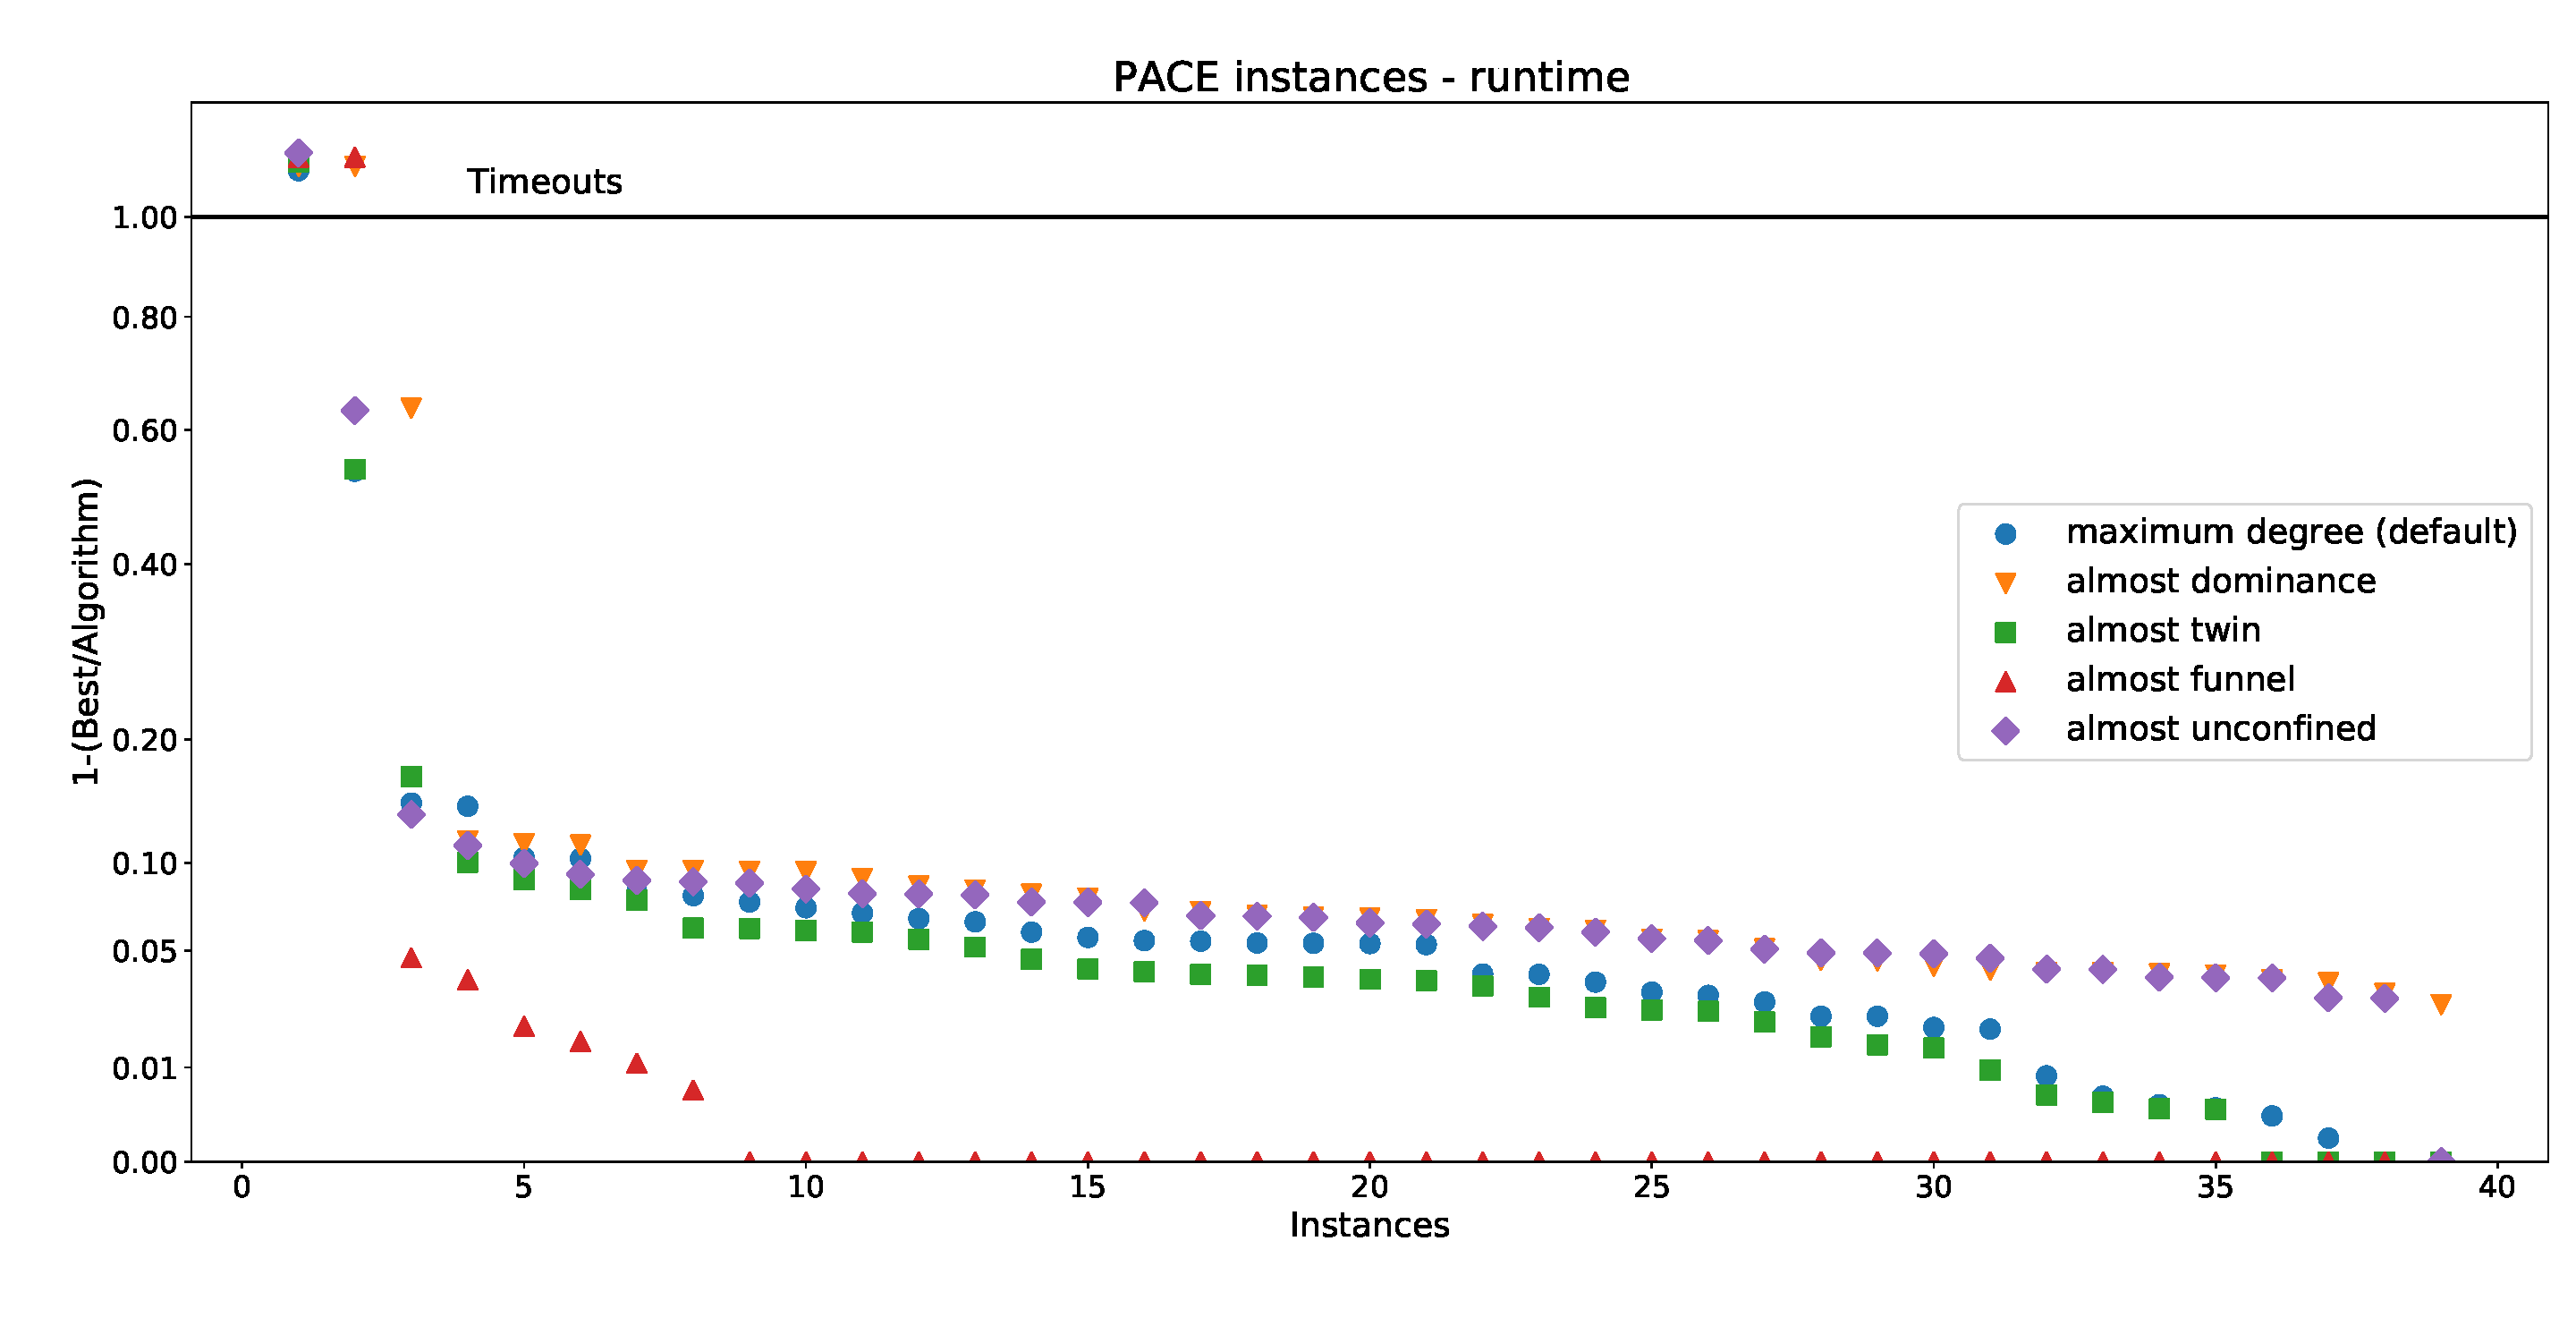
\includegraphics[width=\textwidth]{images/plots/a2_pace_t}
		\caption{runtime}
	\end{subfigure}
	\begin{subfigure}{1\textwidth}
		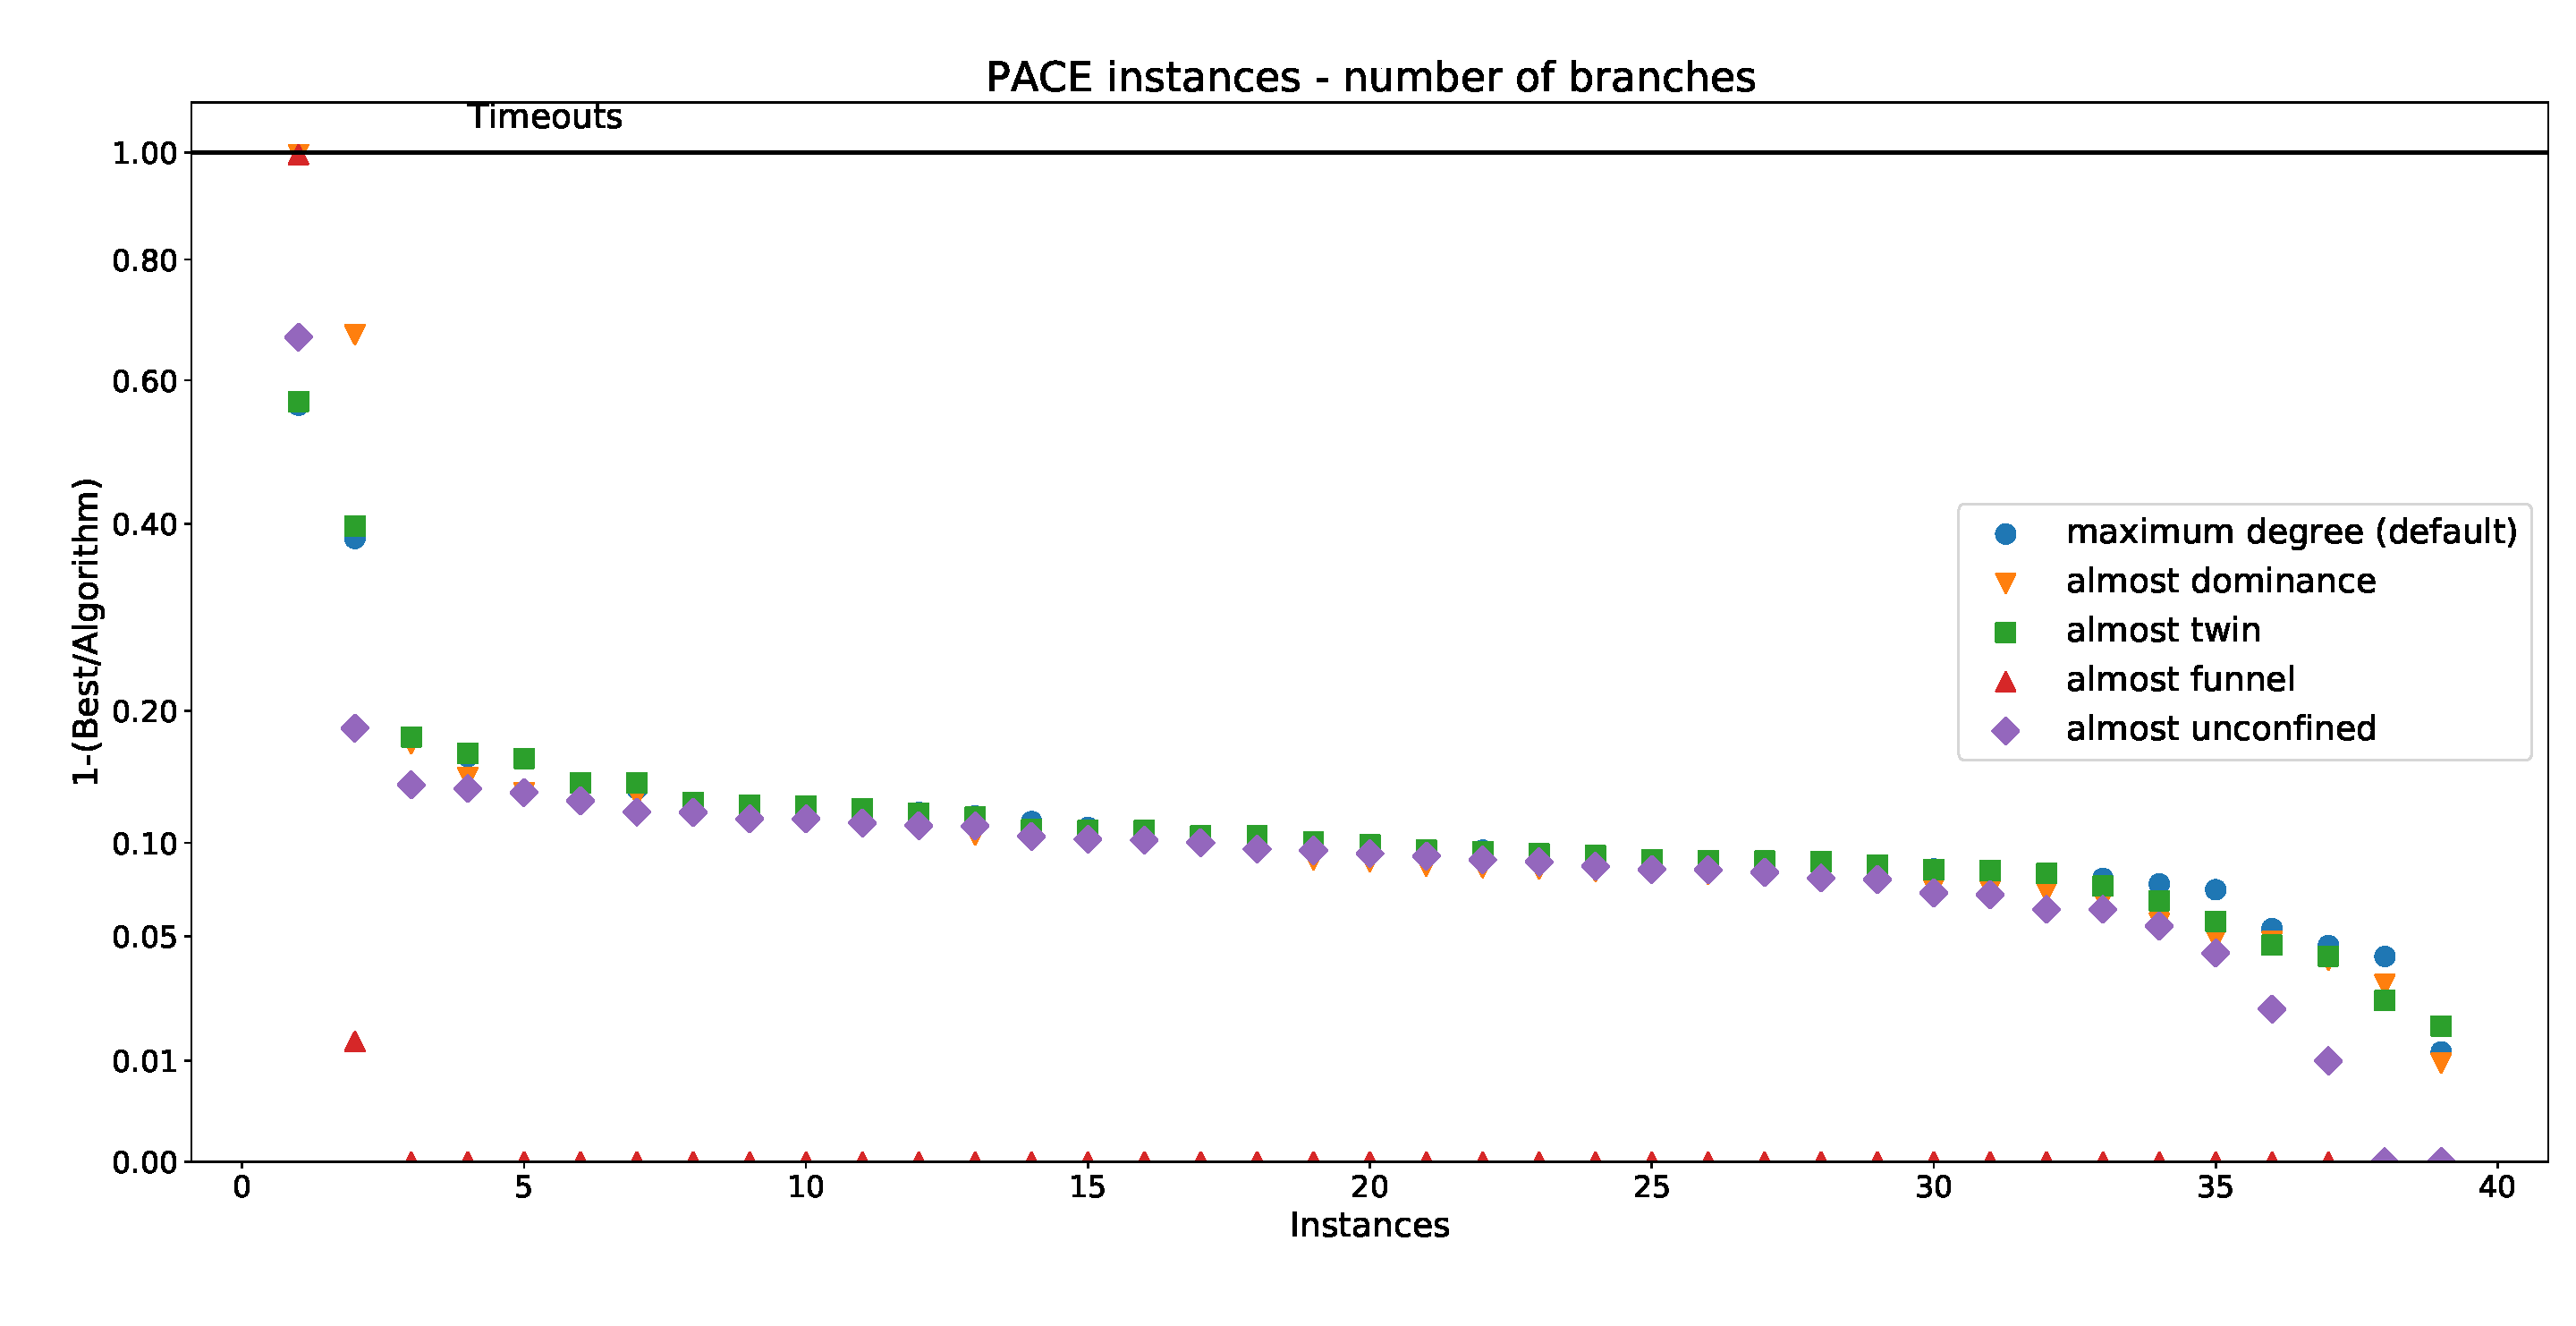
\includegraphics[width=\textwidth]{images/plots/a2_pace_b}
		\caption{number of branches}
	\end{subfigure}
	\caption{Performance plots of branching strategies targeting reductions on PACE instances}
	\label{111}
\end{figure}
\begin{figure}[hbt!]
	\begin{subfigure}{1\textwidth}
		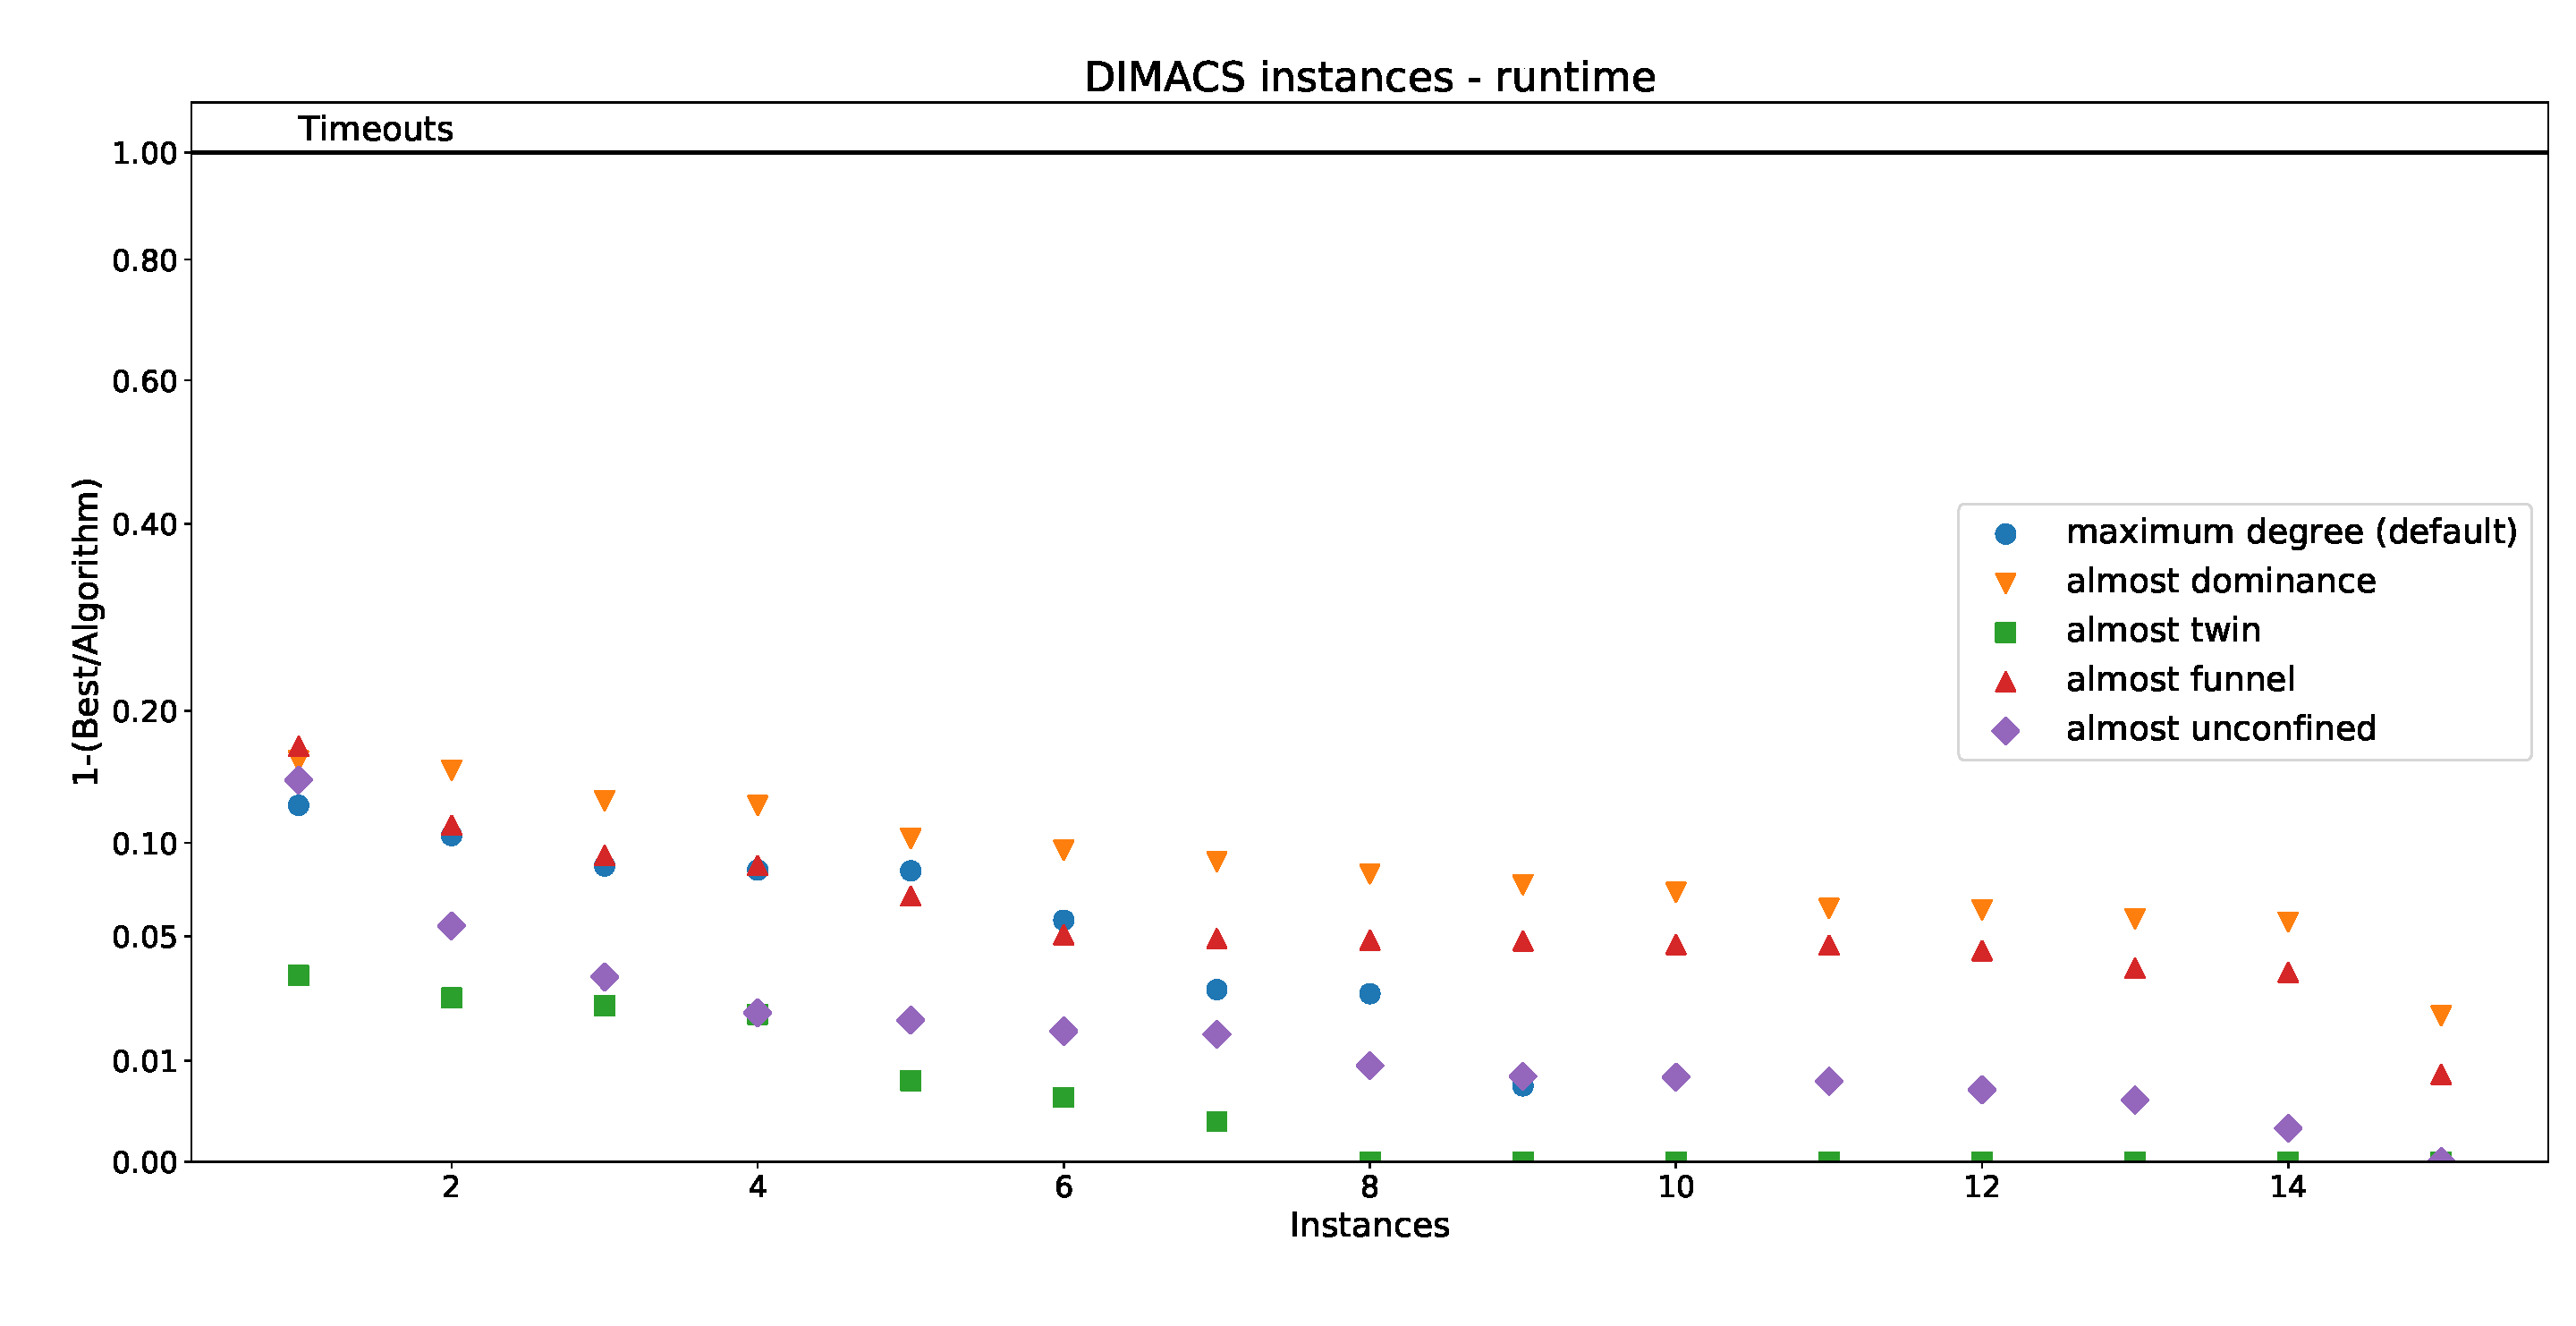
\includegraphics[width=\textwidth]{images/plots/a2_dimacs_t}
		\caption{runtime}
	\end{subfigure}
	\begin{subfigure}{1\textwidth}
		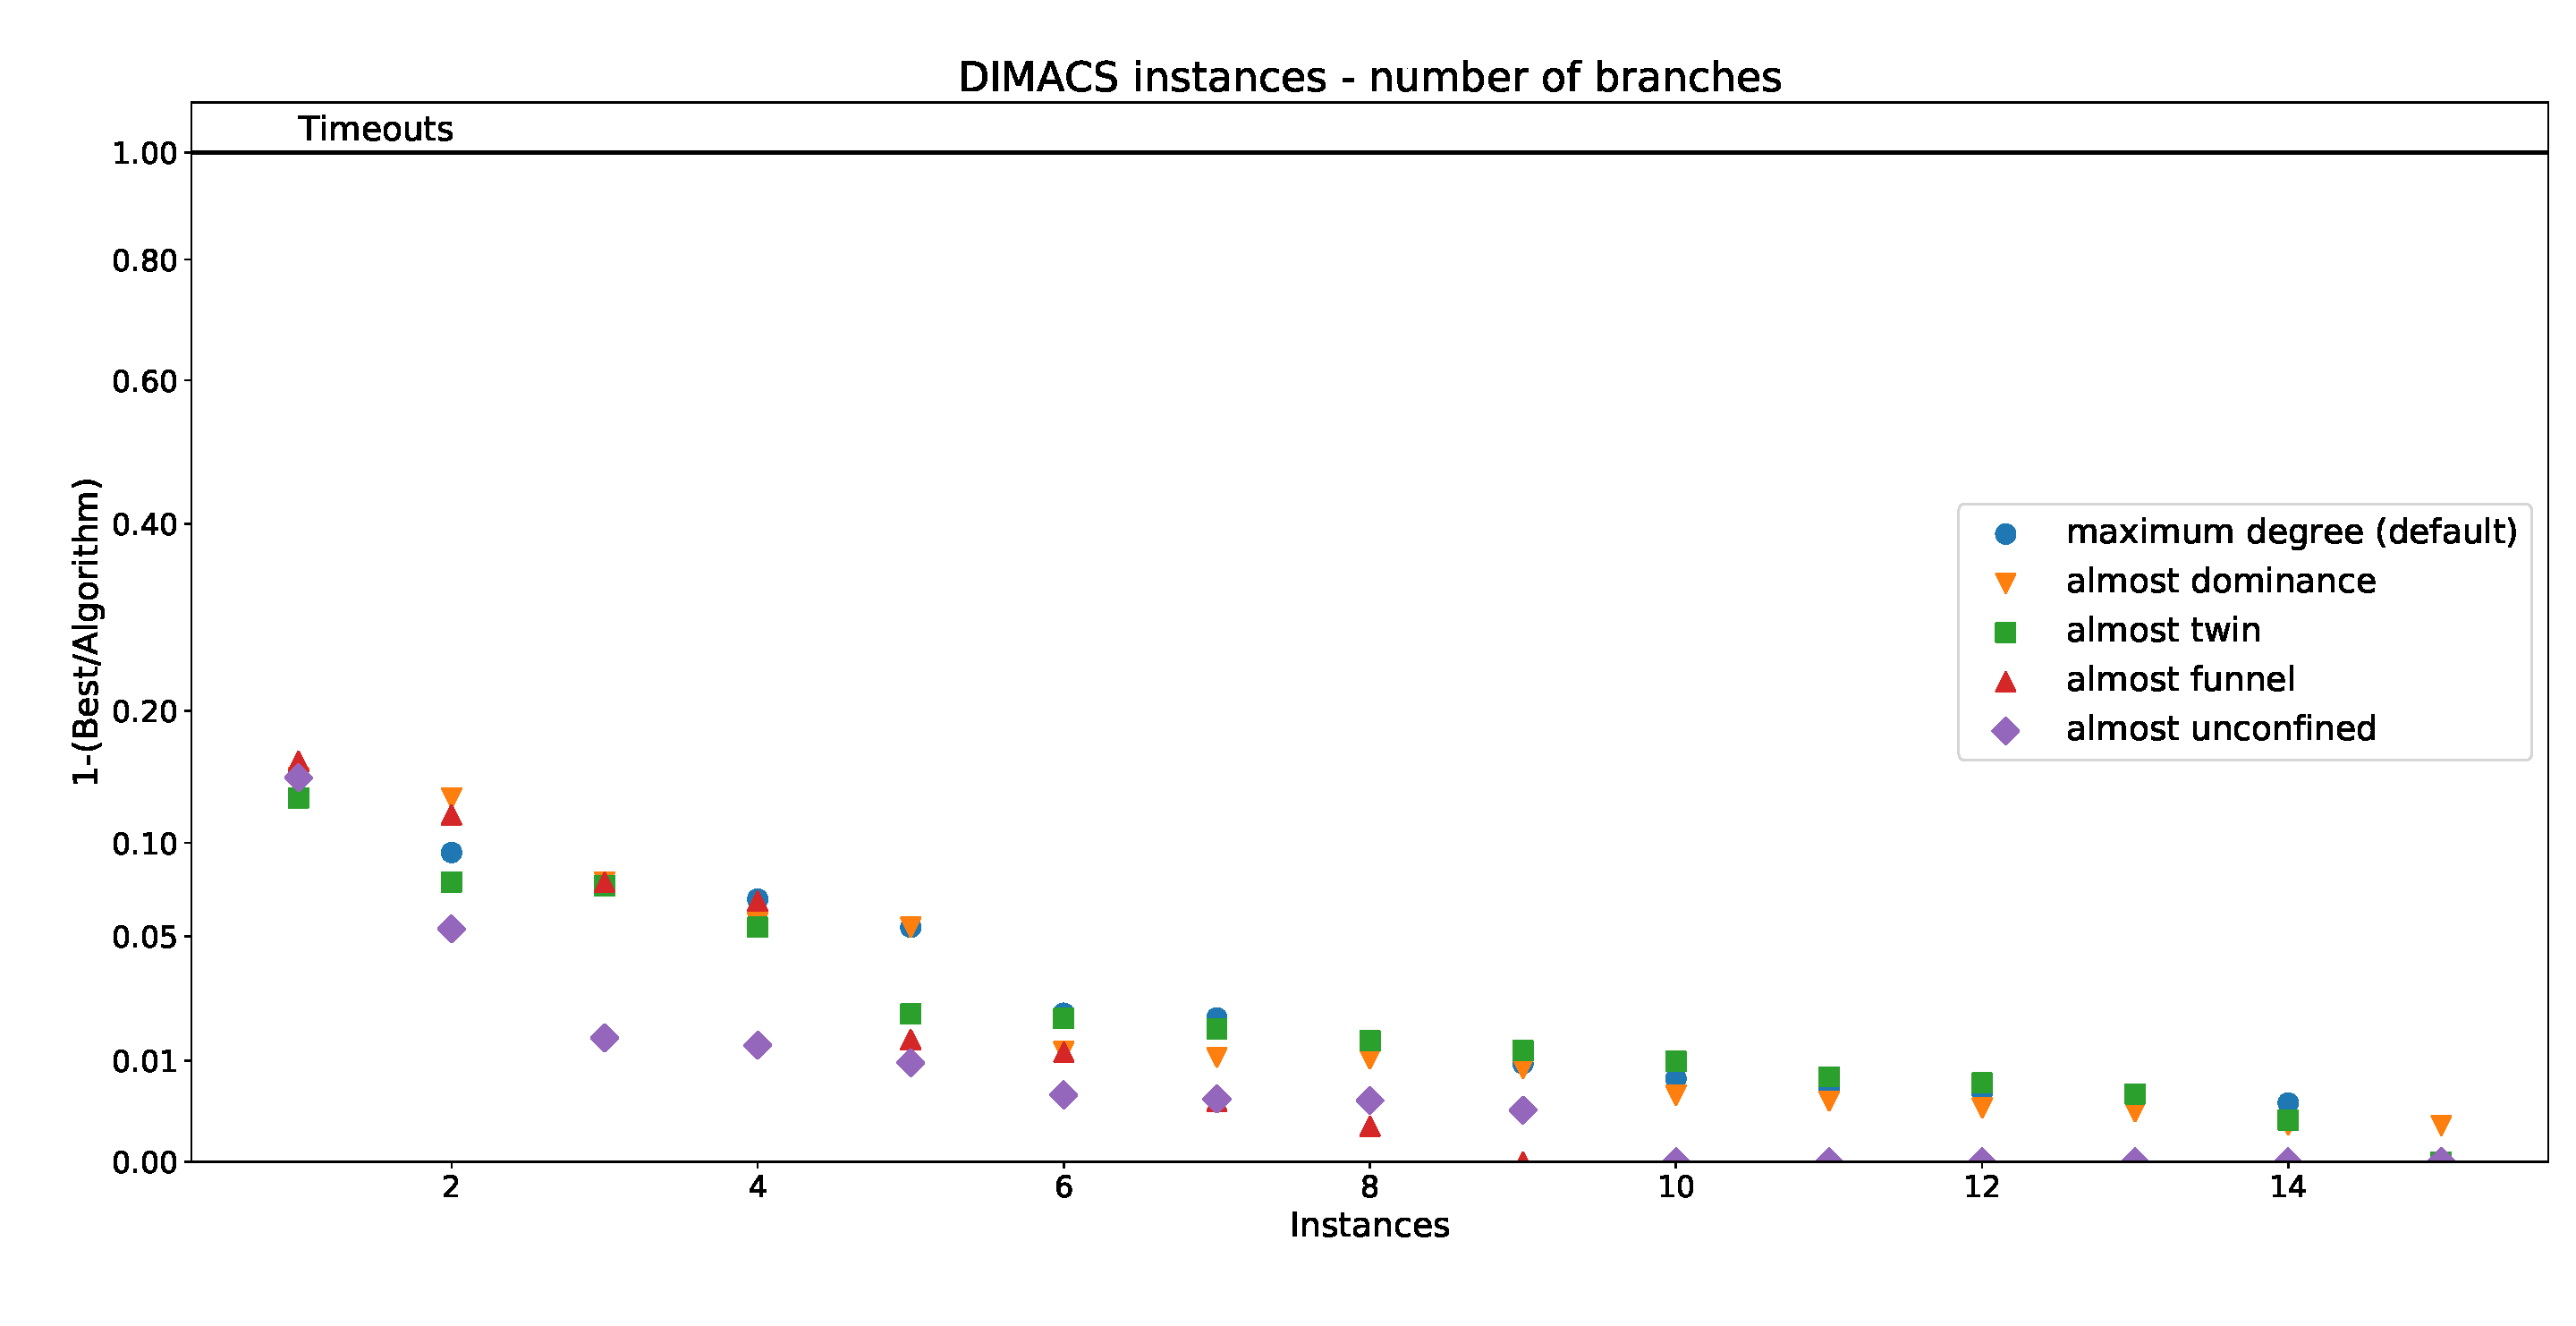
\includegraphics[width=\textwidth]{images/plots/a2_dimacs_b}
		\caption{number of branches}
	\end{subfigure}
	\caption{Performance plots of branching strategies targeting reductions on DIMACS instances}
\end{figure}
\begin{figure}[hbt!]
	\begin{subfigure}{1\textwidth}
		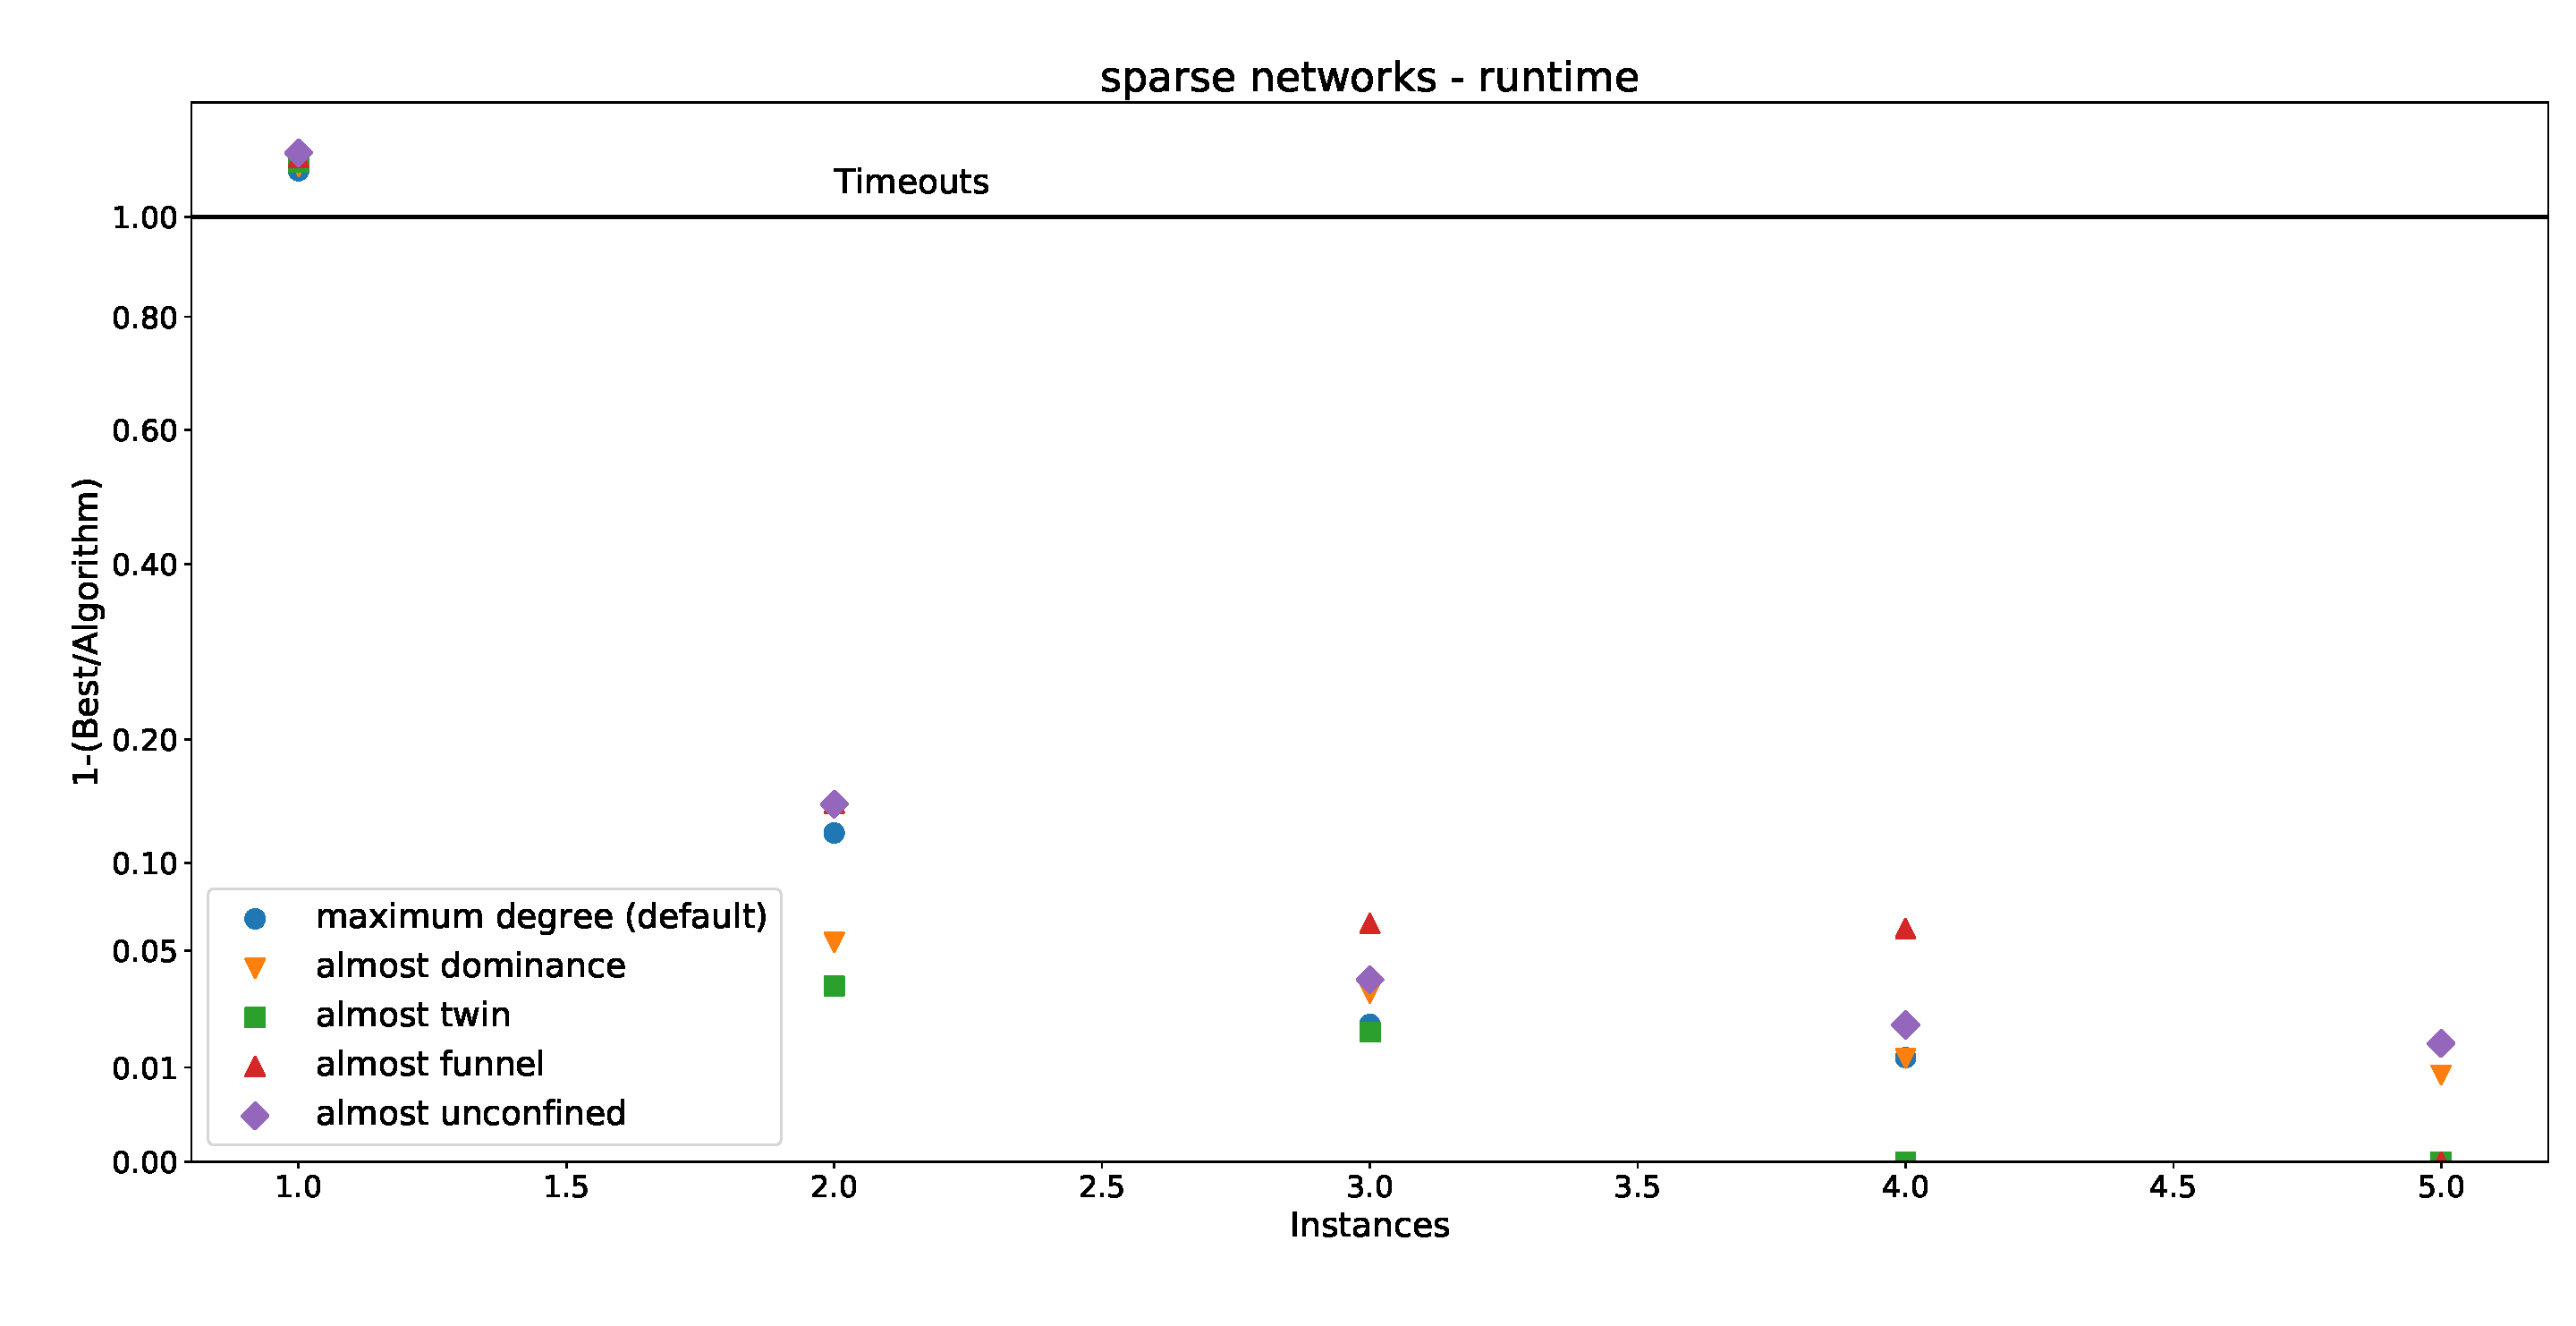
\includegraphics[width=\textwidth]{images/plots/a2_sn_t}
		\caption{runtime}
	\end{subfigure}
	\begin{subfigure}{1\textwidth}
		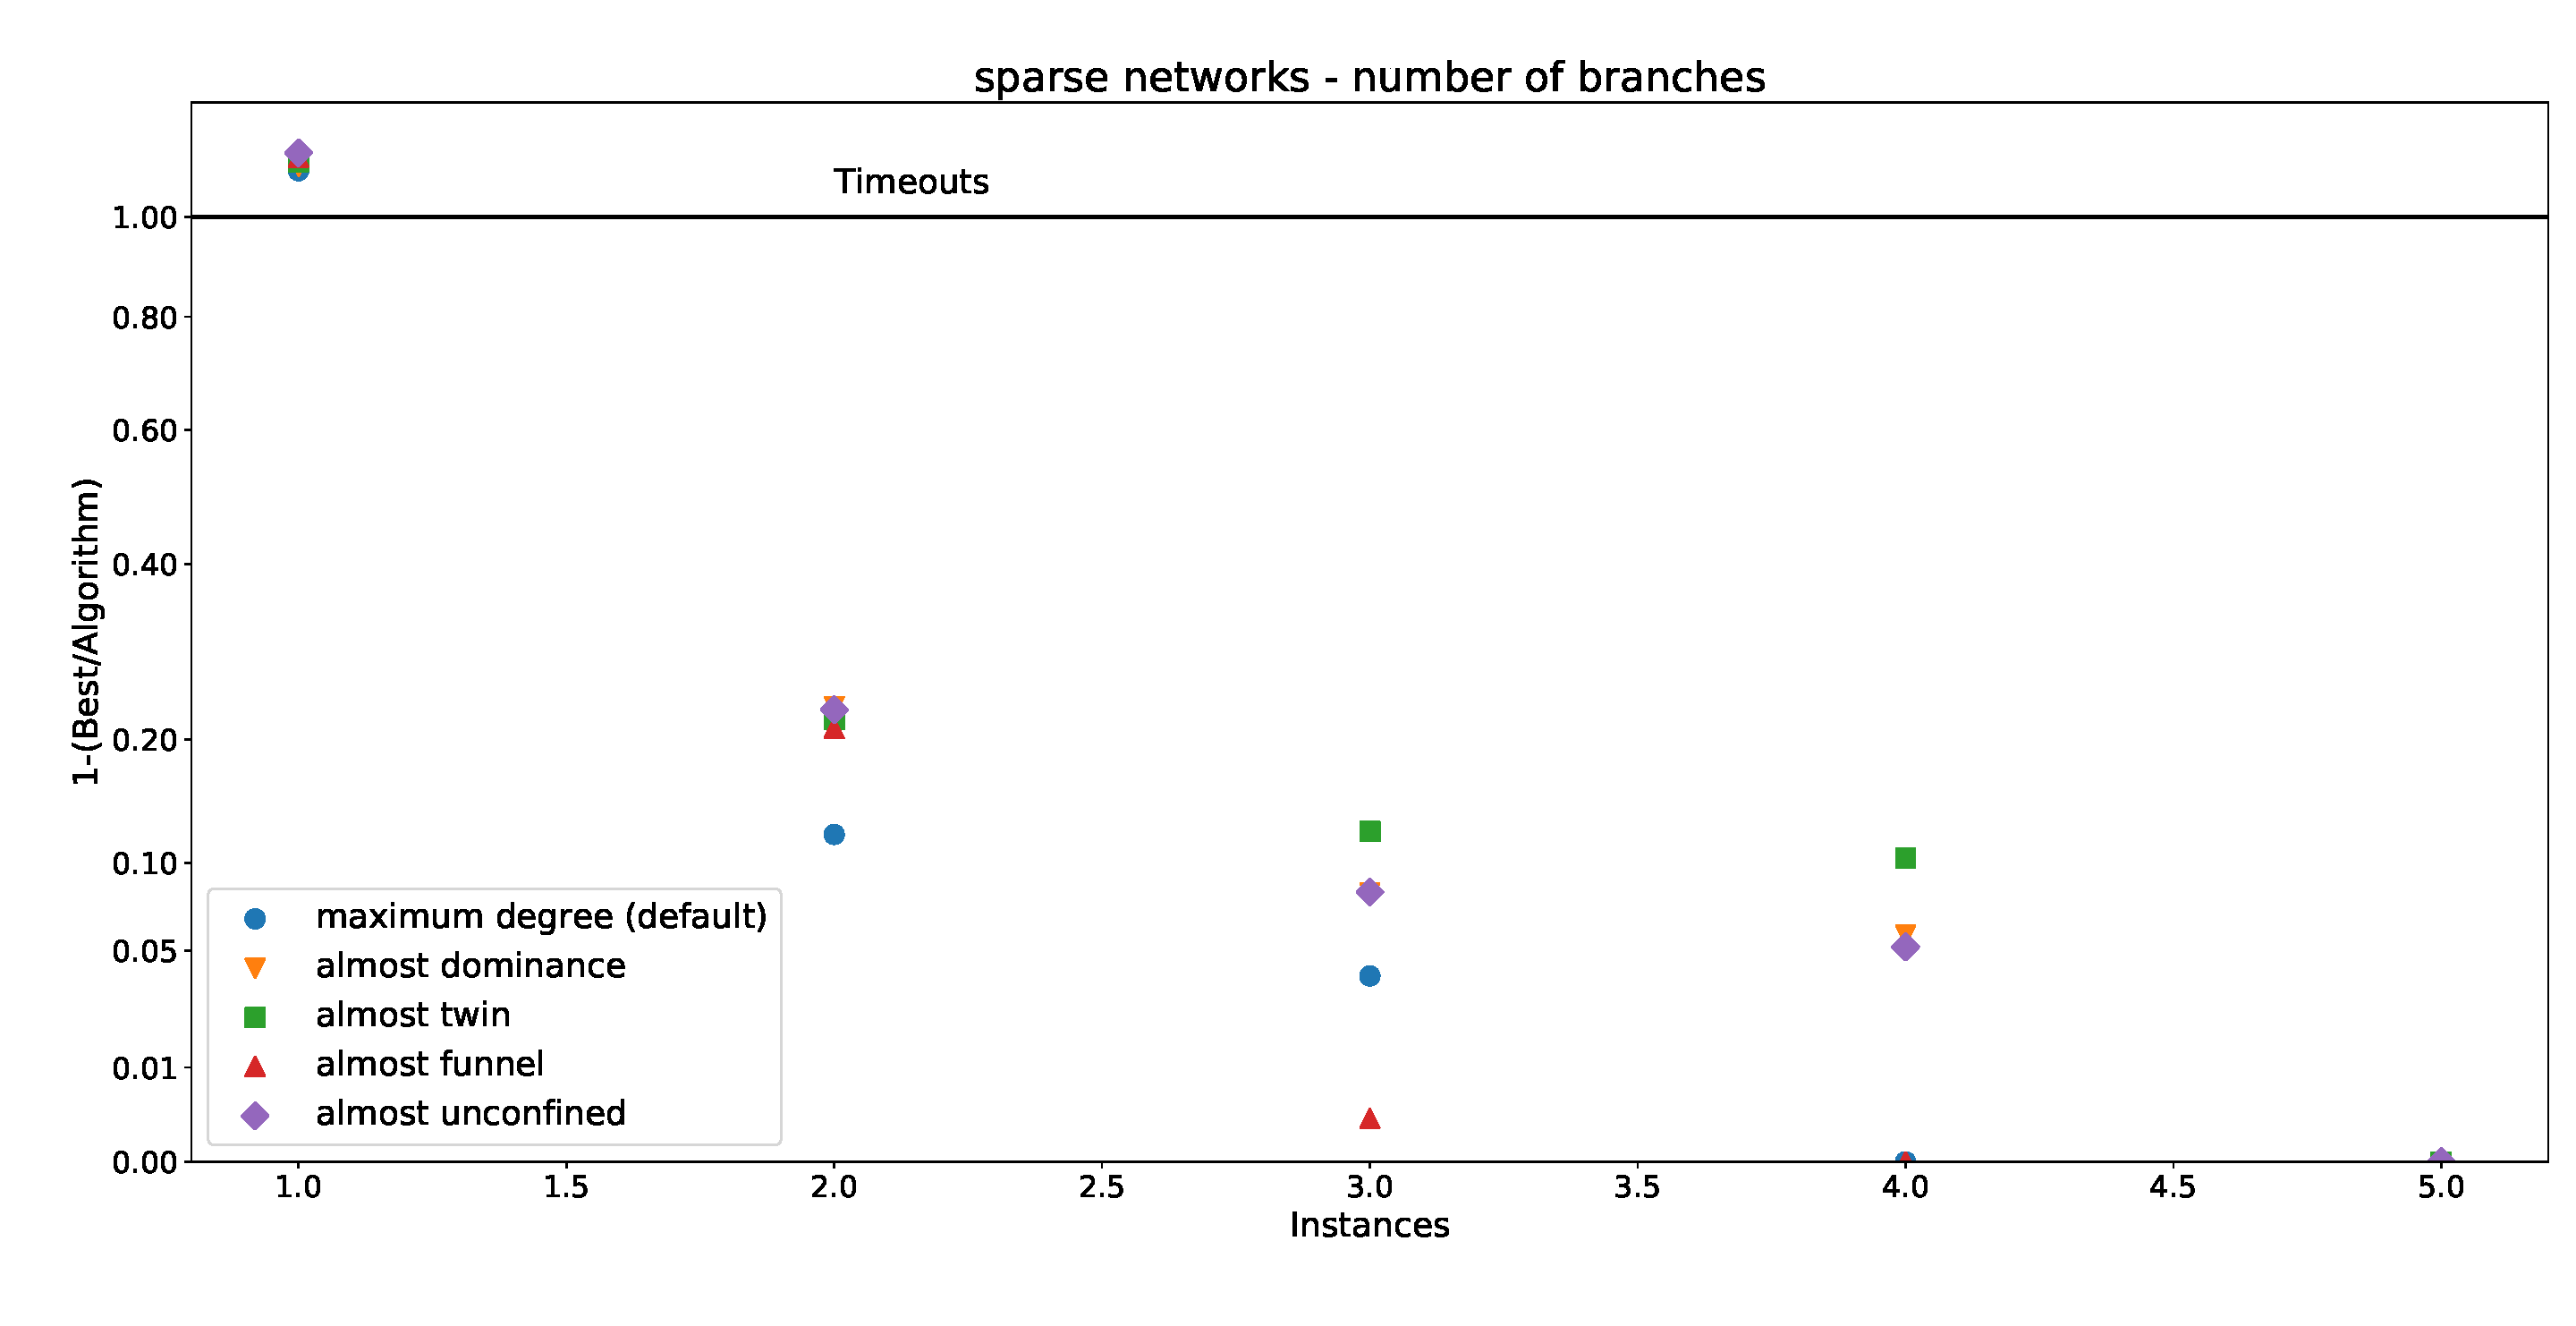
\includegraphics[width=\textwidth]{images/plots/a2_sn_b}
		\caption{number of branches}
	\end{subfigure}
	\caption{Performance plots of branching strategies targeting reductions on sparse networks}
\end{figure}

\begin{figure}[hbt!]
	\begin{subfigure}{1\textwidth}
		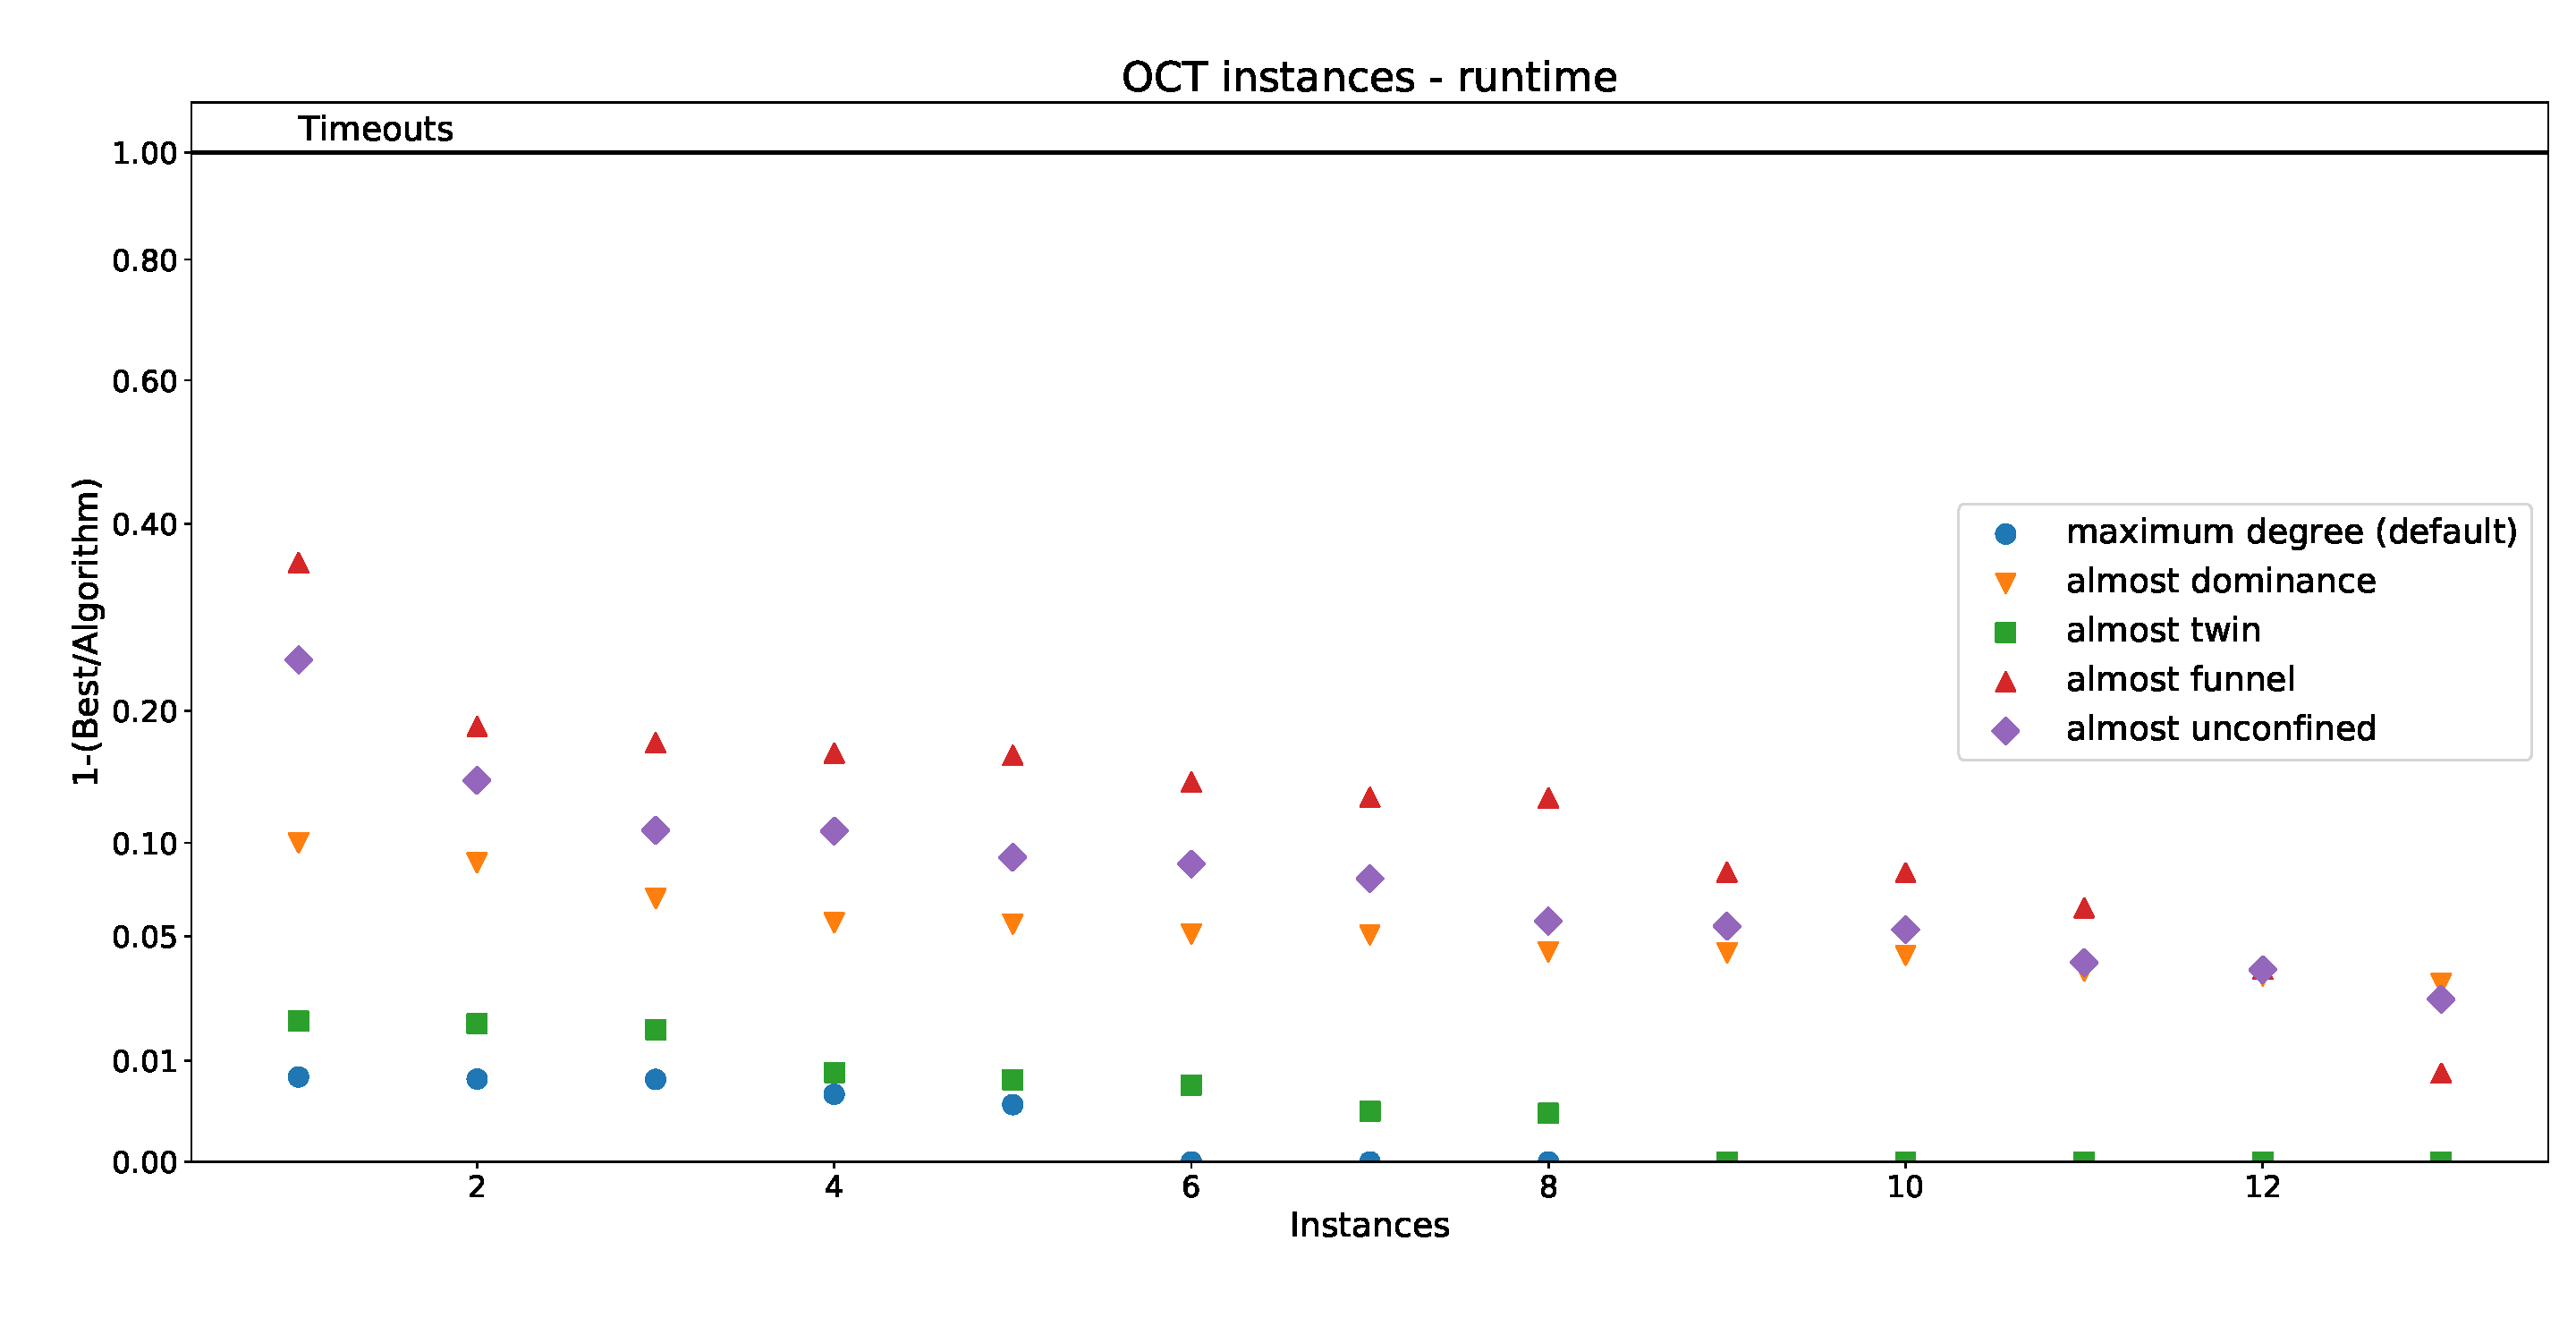
\includegraphics[width=\textwidth]{images/plots/a2_oct_t}
		\caption{runtime}
	\end{subfigure}
	\begin{subfigure}{1\textwidth}
		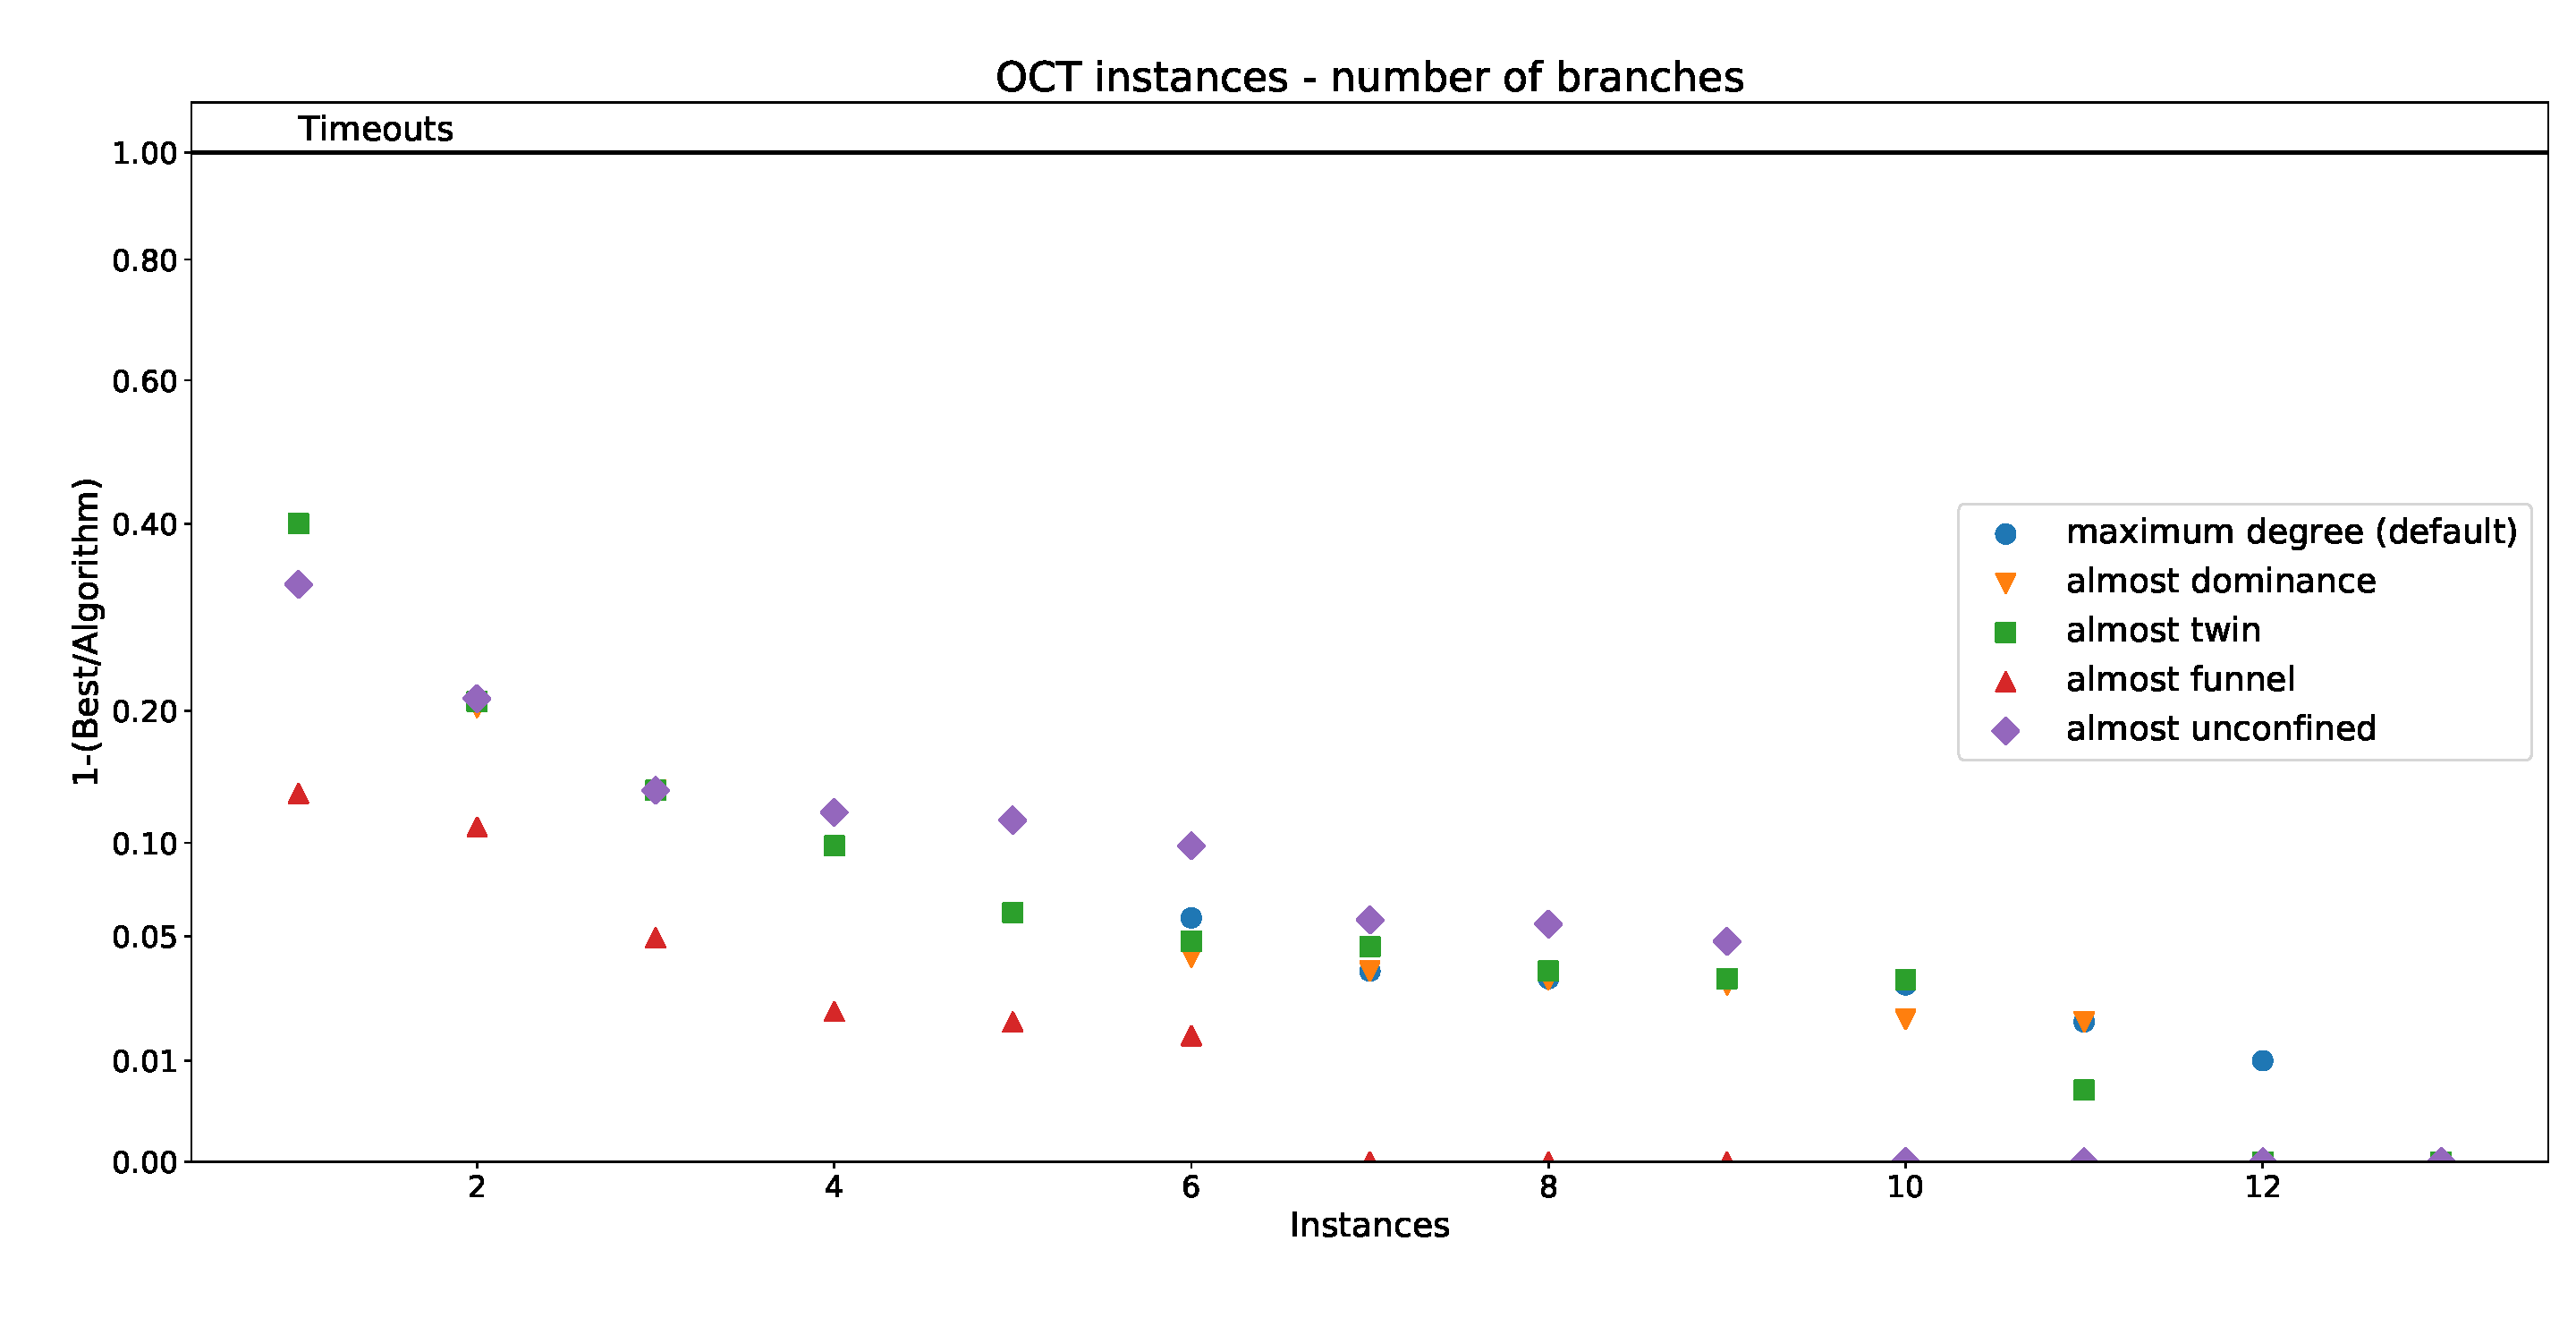
\includegraphics[width=\textwidth]{images/plots/a2_oct_b}
		\caption{number of branches}
	\end{subfigure}
	\caption{Performance plots of branching strategies targeting reductions on graphs obtained from OCT instances}
\end{figure}

\begin{figure}[hbt!]
	\begin{subfigure}{1\textwidth}
		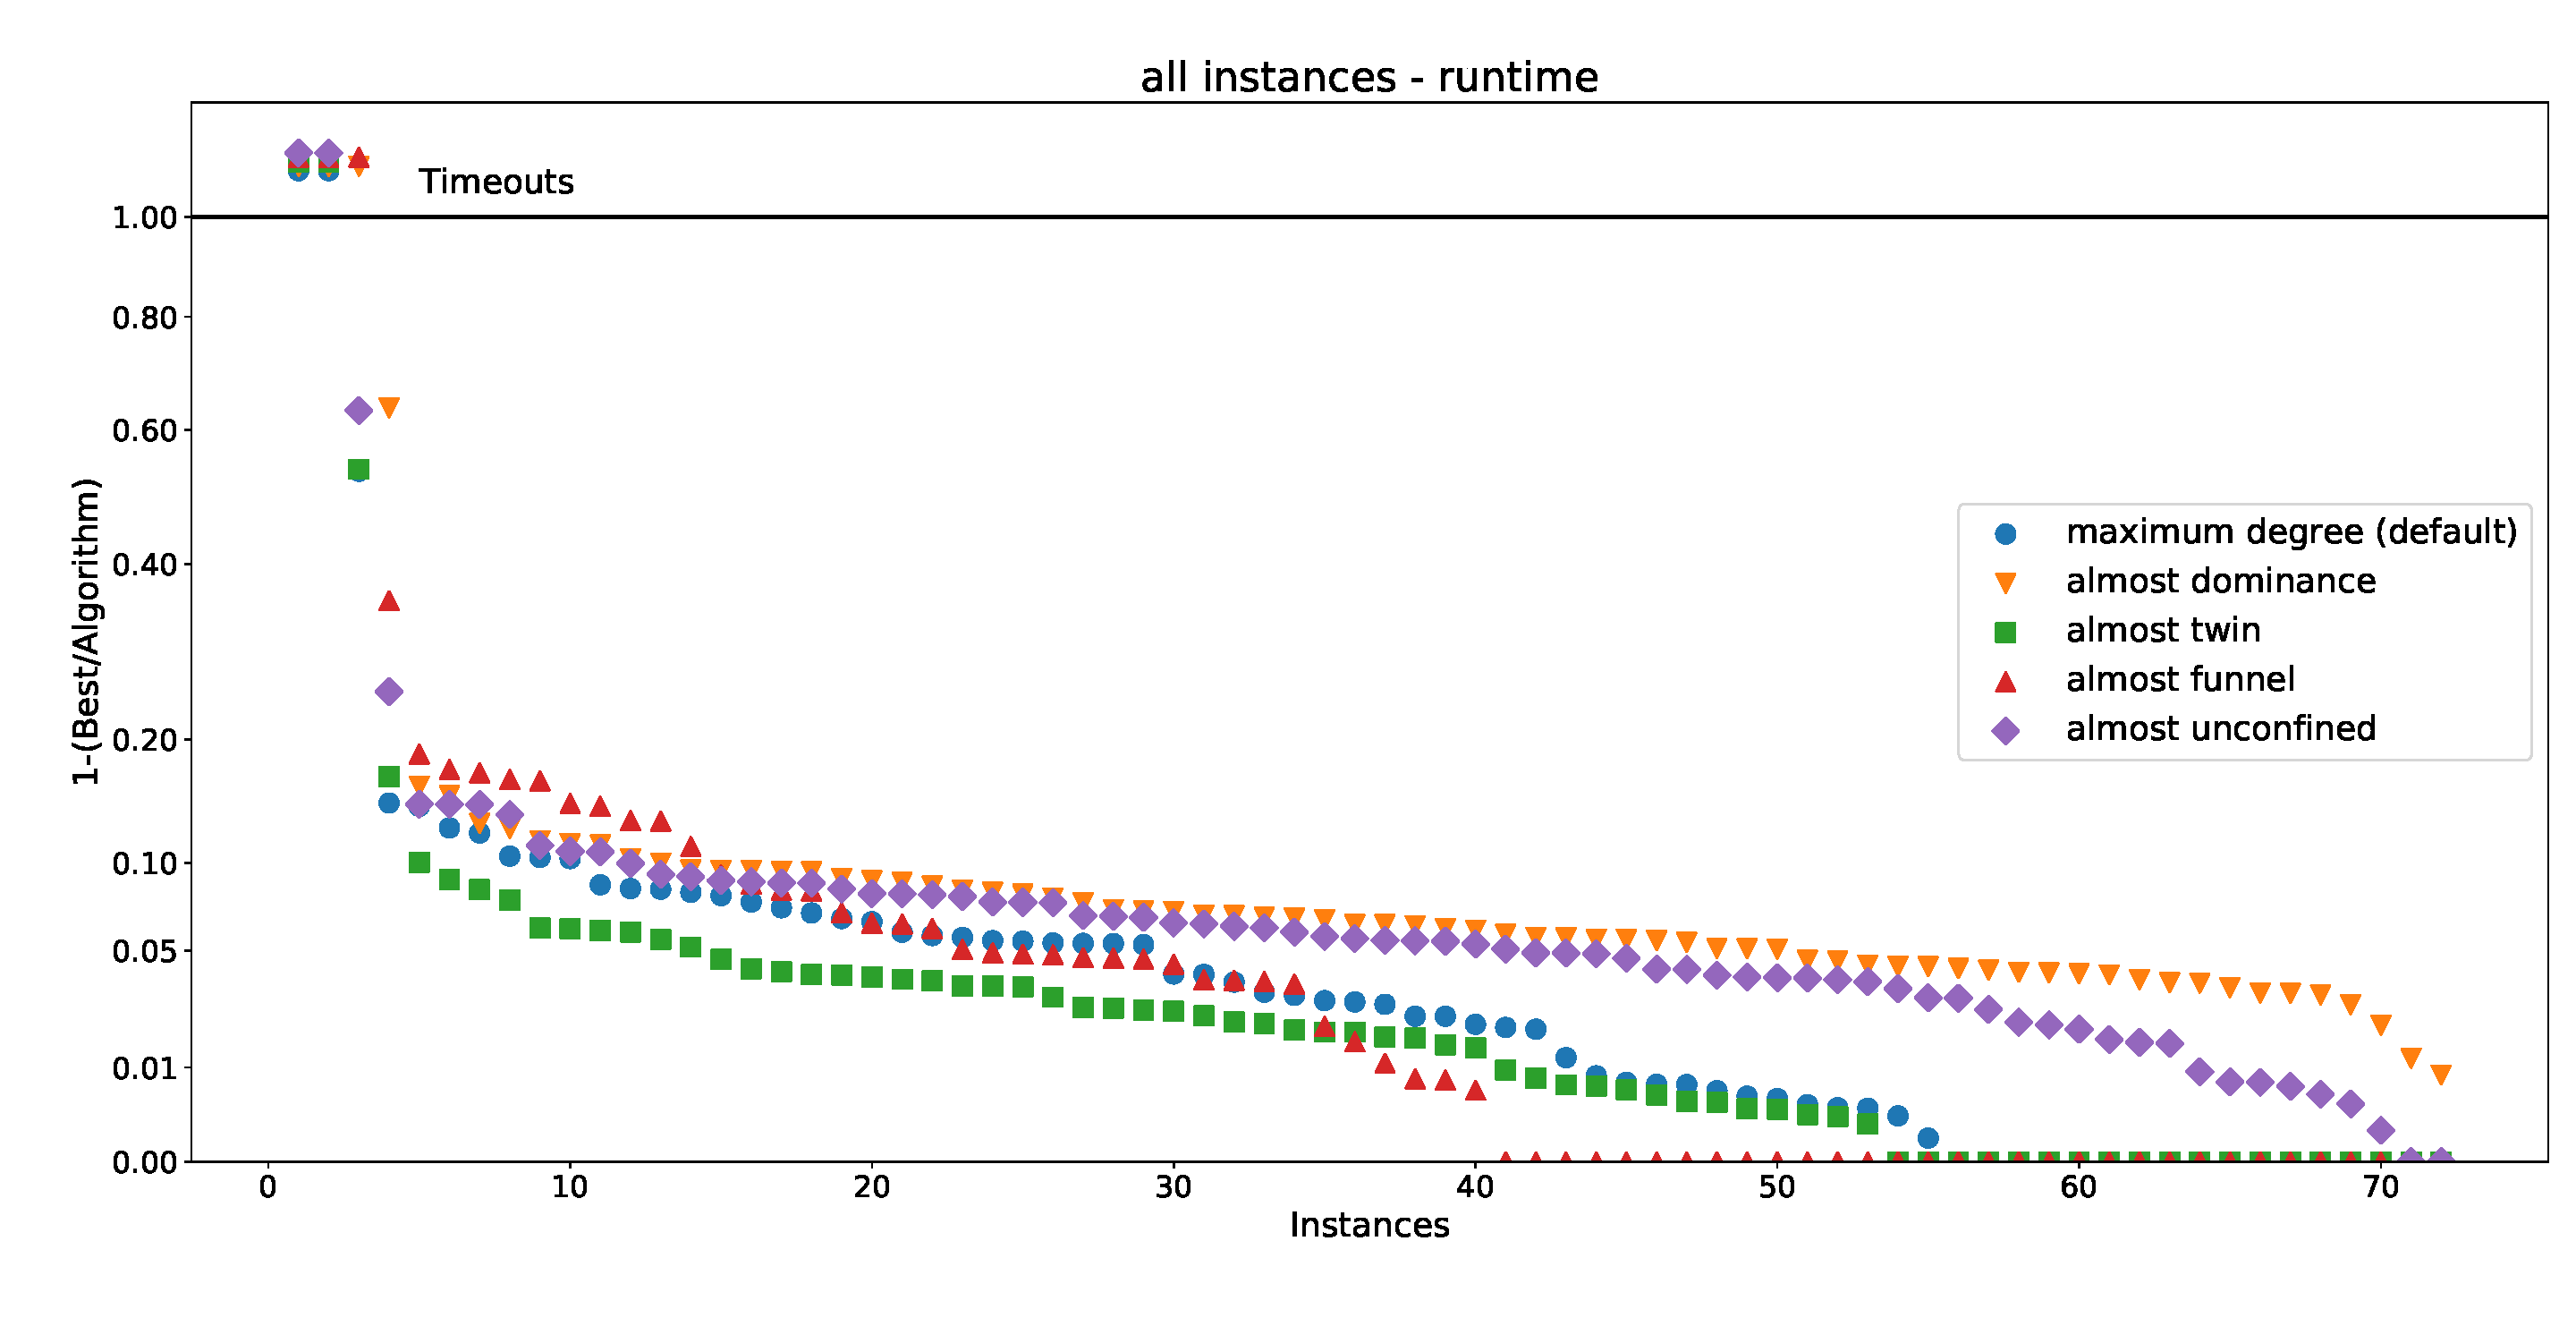
\includegraphics[width=\textwidth]{images/plots/a2_all_t}
		\caption{runtime}
	\end{subfigure}
	\begin{subfigure}{1\textwidth}
		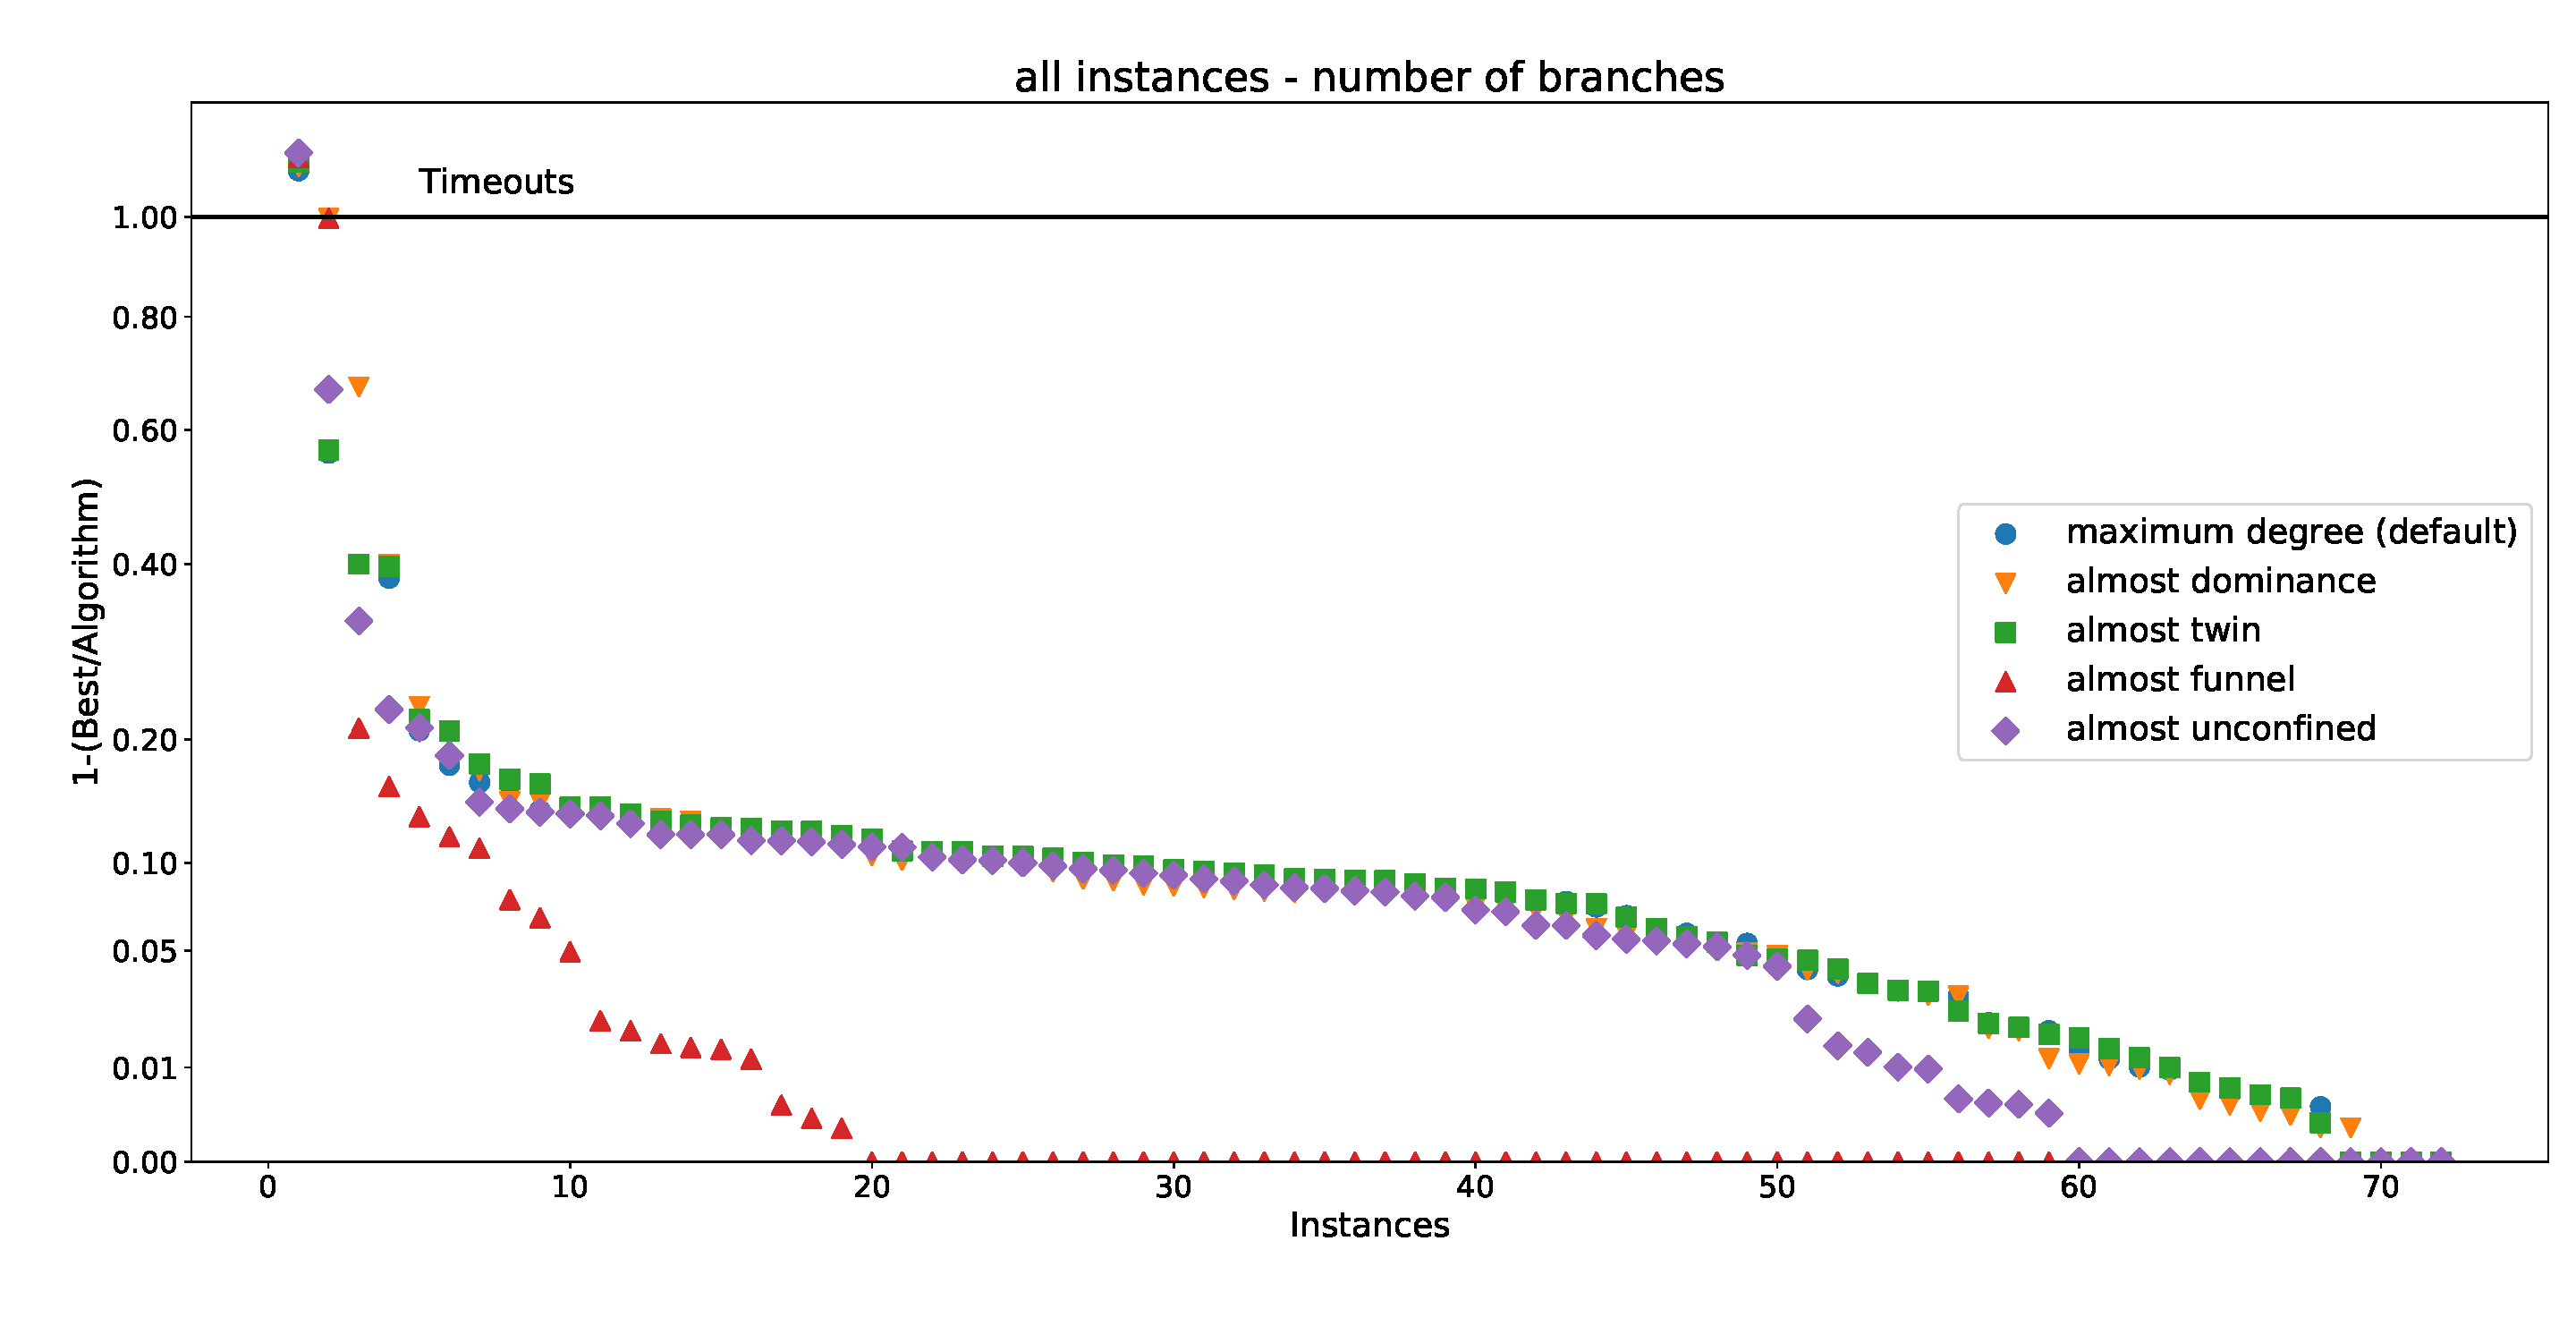
\includegraphics[width=\textwidth]{images/plots/a2_all_b}
		\caption{number of branches}
	\end{subfigure}
	\caption{Performance plots of branching strategies targeting reductions on all instances}
	\label{222}
\end{figure}

\clearpage

%%%%%%%%%%%%%%%%%%%%%%%%%%%%%%%%%%%%%%%%%%%%%%%%%%%%%%%%%%%%%%%%%%%%%%

\section{Conclusion and Future Work} \label{sec6}
\subsection{Conclusion}

In this thesis, we examined multiple branching strategies for a branch and reduce maximum independent set algorithm. Essentially, we evaluated two different approaches. The first approach is to branch on vertices that decompose the graph. Following this approach we presented three different branching strategies. All of them proved to be effective on sparse networks, that can easily be decomposed by branching. However, this approach does not work very well on denser graphs with low skewness, i.e., graphs with a more symmetric degree distribution. The reason for this is that on those instances small and at the same time reasonably balanced separators are rarely found. Furthermore, those graphs contain many vertices of high degree. Hence, the greedy strategy of branching on vertices of maximum degree (i.e., the default strategy) is overall more competitive than on sparse graphs. In summary, we ascertained that decomposing a graph by branching can drastically reduce the total number of branching steps needed to solve a suitable instance, and therefore boost the runtime of the algorithm greatly.

\paragraph{}
Our second approach concerns branching on vertices so that reduction rules become applicable afterwards. For sparse networks, branching on vertices that prevent twin reductions performs better than the default strategy in all cases. The reason for this is that the average degree in those graphs is low, and therefore almost twins are found quite often. Stallmann et al. \cite{Stallmann} showed that the dominance and unconfined reduction rules are highly effective on dense graphs with a high degree variation. Therefore, the reduction step prior to branching is key to minimizing the complexity of those instances. In fact, our experiments show that using branching strategies, which enable the application of the dominance and unconfined reduction rules, in many cases decreases the total number of branching steps on graphs displaying those properties (e.g. DIMACS an PACE instances). Unfortunately, in our implementations the reduction in branching steps is very small and therefore does not compensate for the additional time overhead of finding suitable branching vertices. Here, the situation is different with the branching strategy utilizing funnel reduction, which has proven to be the best strategy for almost all PACE instances. In conclusion, we believe that targeting reduction rule is very promising for reducing the number of branching steps on highly connected dense graphs.

\subsection{Future Work} \label{sec7}
In this subsection we discuss possible options to further develop and optimize our branching strategies described in this thesis. Moreover, we outline new ideas for alternate approaches which may pave the way for future progress in this field.

\paragraph{}
As already mentioned in Section \ref{sec5}, the aim of this thesis was not to optimize certain strategies down to the last detail. Instead, we examined a range of different strategies following multiple approaches to comparatively evaluate the basic potential of those solutions. For this purpose we also considered the total number of branching steps. Hence, for most of our implementations there is a lot of leeway to optimize runtime. For instance, we did not implement our own variant of a preflow push algorithm, but instead used an implementation from the KaHIP library \cite{KAHIP}. Consequently, the current graph must be converted to the format used by the KaHIP library at each branching step creating additional overhead. Another possible optimization regarding this branching strategy is to find better choices for the source and sink vertices ($s$ and $t$) utilized in calculating the edge cut.  

\paragraph{}
Utilizing nested dissection for branching has proven to be competitive to the default strategy, at least on DIMACS instances. Therefore, we see potential for further optimization involving this strategy. Like branching using edge cuts, we must convert the graph into another format in order to use the nested dissection algorithm from the METIS library. This, however, causes a non-negligible runtime overhead. Furthermore, the METIS library provides many settings that can be used to tweak the nested dissection algorithm and, thus, the branching strategy. Tuning our edge cut based strategy, we already showed that the balance of a separator has a big influence on the effectiveness of a strategy. Thus, it might be interesting to examine whether there is a tradeoff between the balance of the bipartitions and the size of the separators used in the nested dissection algorithm. Also, a partitioning algorithm that produces higher quality bipartitions at the cost of computation time could improve the strategy further. 

\paragraph{}
Our experiments show that branching strategies which target reduction rules are generally very effective even though our respective implementations are rather simple. For instance, when searching vertices that enable reduction rules upon removal, we assume that the respective vertex is eliminated by branching. However, we do not take into consideration that the neighborhood of a vertex is also removed from the graph when the vertex is included into the current solution by branching. Therefore, we believe that there is a lot of potential for further development in following this approach.

\paragraph{}
Furthermore, we believe that the branching concept aiming at the application of reduction rules can also be adopted for the packing branching rule. During kernelization one can find vertices whose removal forces the reduction of other vertices to satisfy the constraints resulting from the packing rule. It might be worth branching on such vertices, if their degree is large enough.

\paragraph{}
Unfortunately, our test results show that branching on articulation points is ineffective most of the time. However, there are two sparse network instances for which this strategy produces results being orders of magnitude better than default branching. Unfortunately, we did not find a satisfying explanation for these outliers. Analyzing different graph parameters on the initial kernel of those instances showed that one of the outliers seem to have a significantly higher average betweenness centrality than other sparse network instances. However, when looking at all instances together, we could not find any correlation between the effectiveness of this branching strategy and betweenness centrality. Nevertheless, we believe that exploring relations between the effectiveness of branching strategies and graph characteristics can help optimizing existing strategies or even finding new ones. Stallmann et al. \cite{Stallmann} previously proposed a similar approach involving reduction rules. They showed that there is a correlation between certain graph parameters and the effectiveness of the reduction rules. Furthermore, they presented an improved variant of the branch and reduce algorithm by Akiba and Iwata \cite{AkibaIwata}, where they only apply a subset of reduction rules based on simple graph parameters of the instance. This way, they reduced kernelization time and significantly speeded up the algorithm.

\paragraph{}
During the testing of our branching strategies we discovered evidence that branches at lower depth of recursion have a much greater influence on the runtime of the algorithm than such at a higher depth. For this reason, it might be worth investing much execution time into finding branching vertices at the start of recursion, compensating for the time spent by using a simple branching strategy at higher depth of recursion.

\clearpage

\appendix{}
\section{Benchmark Instances}

Table \ref{tab:bench_instances} lists all of our benchmark instances along with the source we obtained them from.

\begin{table}[hbt!]
	\centering
	\begin{tabular}{l|c|r}
		Name & type & source \\ \hline
		Inst. \texttt{36} to \texttt{75} & PACE & \cite{PACE_INST, pace} \\ \hline
		\texttt{brock200\_1} & DIMACS & \cite{DIMACS} \\
		\texttt{brock200\_2} & DIMACS & \cite{DIMACS} \\
		\texttt{brock200\_3} & DIMACS & \cite{DIMACS} \\
		\texttt{brock200\_4} & DIMACS & \cite{DIMACS} \\
		\texttt{gen200\_p0.9\_44} & DIMACS & \cite{DIMACS} \\
		\texttt{gen200\_p0.9\_55} & DIMACS & \cite{DIMACS} \\
		\texttt{hamming6-4} & DIMACS & \cite{DIMACS} \\
		\texttt{hamming8-4} & DIMACS & \cite{DIMACS} \\
		\texttt{johnson8-2-4} & DIMACS & \cite{DIMACS} \\
		\texttt{johnson8-4-4} & DIMACS & \cite{DIMACS} \\
		\texttt{johnson16-2-4} & DIMACS & \cite{DIMACS} \\
		\texttt{p\_hat300-1} & DIMACS & \cite{DIMACS} \\
		\texttt{p\_hat300-2} & DIMACS & \cite{DIMACS} \\
		\texttt{p\_hat500-1} & DIMACS & \cite{DIMACS} \\
		\texttt{p\_hat500-2} & DIMACS & \cite{DIMACS} \\ \hline	
		\texttt{web-Stanford} & sparse network & \cite{WEB_INST} \\
		\texttt{web-BerkStan} & sparse network & \cite{WEB_INST} \\
		\texttt{web-NotreDame} & sparse network & \cite{WEB_INST2} \\
		\texttt{as-Skitter} & sparse network & \cite{WEB_INST3} \\
		\texttt{libimseti} & sparse network & \cite{WEB_INST4} \\ \hline	
		\texttt{afro-17} & OCT & \cite{OCT}	\\			
		\texttt{afro-19} & OCT & \cite{OCT}	\\			
		\texttt{afro-28} & OCT & \cite{OCT}	\\			
		\texttt{afro-29} & OCT & \cite{OCT}	\\				
		\texttt{afro-32} & OCT & \cite{OCT}	\\			
		\texttt{afro-38} & OCT & \cite{OCT}	\\			
		\texttt{afro-39} & OCT & \cite{OCT}	\\		
		\texttt{afro-40} & OCT & \cite{OCT}	\\			
		\texttt{afro-41} & OCT & \cite{OCT}	\\			
		\texttt{afro-42} & OCT & \cite{OCT}	\\				
		\texttt{afro-45} & OCT & \cite{OCT}	\\			
		\texttt{afro-46} & OCT & \cite{OCT}	\\			
		\texttt{afro-54} & OCT & \cite{OCT}	\\
		
	\end{tabular}
	\caption{Benchmark instances used in this thesis}
	\label{tab:bench_instances}
	
\end{table}
\clearpage
Table \ref{tab:tune_instances} lists all instances used for parameter tuning.

\begin{table}[hbt!]
	\centering
	\begin{tabular}{l|c|r}
		Name & type & source \\ \hline
		Inst. \texttt{41} to \texttt{45} & PACE & \cite{PACE_INST, pace} \\ 
		Inst. \texttt{51} to \texttt{55} & PACE & \cite{PACE_INST, pace} \\\hline
		\texttt{brock200\_2} & DIMACS & \cite{DIMACS} \\
		\texttt{brock200\_3} & DIMACS & \cite{DIMACS} \\
		\texttt{gen200\_p0.9\_44} & DIMACS & \cite{DIMACS} \\
		\texttt{hamming6-4} & DIMACS & \cite{DIMACS} \\
		\texttt{johnson8-2-4} & DIMACS & \cite{DIMACS} \\
		\texttt{johnson16-2-4} & DIMACS & \cite{DIMACS} \\
		\texttt{p\_hat300-1} & DIMACS & \cite{DIMACS} \\
		\texttt{p\_hat500-2} & DIMACS & \cite{DIMACS} \\ \hline	
		\texttt{web-Stanford} & sparse network & \cite{WEB_INST} \\
		\texttt{web-BerkStan} & sparse network & \cite{WEB_INST} \\
		\texttt{as-Skitter} & sparse network & \cite{WEB_INST3} \\ \hline	
		\texttt{afro-17} & OCT & \cite{OCT}	\\	
		\texttt{afro-19} & OCT & \cite{OCT}	\\	
		\texttt{afro-32} & OCT & \cite{OCT}	\\	
		\texttt{afro-38} & OCT & \cite{OCT}	\\	
		\texttt{afro-42} & OCT & \cite{OCT}	\\		
	\end{tabular}
	\caption{Benchmark instances used in this thesis}
	\label{tab:tune_instances}
	
\end{table}
\clearpage

\section{Algorithms}

\begin{algorithm}
	\caption{GetArticulationPoints}\label{alg:artic}
	\SetKwFunction{U}{ArticulationPoints}
	\DontPrintSemicolon
	
	\texttt{Global variables:} A set of articulation points $AP$\\
	\KwIn{A graph $G=(V,E)$}
	
	$AP \leftarrow \emptyset$\; 
	$v\leftarrow u\in V$\tcp*{pick arbitrary start vertex}
	$currentDFSnum \leftarrow 1$ ; $rootDeg \leftarrow 0$\;
	\U{G, v, w}	
	\Begin{		
		$\text{label}(v) \leftarrow currentDFSnum$\;
		$currentDFSnum \leftarrow currentDFSnum + 1$\;
		\ForEach{$u\in N(v)\setminus\{w\}$}
		{
			\eIf{$\text{label}(u) = \bot$} 
			{ \If{$v = w$}{$rootDeg \leftarrow rootDeg + 1$\tcp*{$v$ is root}}
				\U{G, u, v}\tcp*{$\{v,u\}$ tree edge}
				$\text{label}(v) = \min\{\text{label}(v),\text{label}(u)\}$\;	
				\If{$\text{label}(u) > \text{label}(v)$}{$AP \leftarrow AP \cup\{v\}$\tcp*{no back edge: $v$ is articulation point}} } 
			{$\text{label}(v) = \min\{\text{label}(v),\text{label}(u)\}$ \tcp*{$\{v,u\}$ back edge}}
		}
		
	}
	\If{$rootDeg < 2$}{$AP \leftarrow AP \setminus \{v\}$\tcp*{root is no articulation point}}
	\Return{$AP$}\;
	\KwOut{the set $AP$ of articulation points}
	
\end{algorithm}

\begin{algorithm}
	\caption{GetSeparatorFromEdgeCut}\label{alg:edge_sep}
	\SetKwFunction{U}{GetSeparatorFromEdgeCut}
	\SetKwFunction{HC}{HopcroftKarp}
	\SetKwFunction{C}{MinCut}	
	\SetKwFunction{MC}{MaxDegVertex}
	\SetKwFunction{AUX}{ConstructAuxiliaryGraph}
	\DontPrintSemicolon
	\KwIn{A graph $G=(V,E)$}
	
	\U{G}	
	\Begin{
		$s\leftarrow \MC{G}$\\ 
		$t\leftarrow \MC{$G-\{s\}$}$\\
		$(S,T)\leftarrow \C{s, t}$\tcp*{utilizes a max flow algorithm}		
		\If{$\frac{|S|}{|V|}<MinBalance\; \lor\; \frac{|T|}{|V|}< MinBalance$}{\Return $\emptyset$\tcp*{cut is to unbalanced}}	
		$G'\leftarrow \AUX{S,T}$ \\
		$U \leftarrow \HC{$G'$}$ \\
		\If{$|U| > MaxSeparatorSize$}{\Return $\emptyset$\tcp*{separator is to large}}	
		\Return $U$
	}
	
	\KwOut{a set of vertices for branching}
	
\end{algorithm}

\begin{algorithm}
	\caption{ExtractSeparators}\label{alg:extract}
	\SetKwFunction{U}{ExtractSeparators}
	\SetKwFunction{A}{GetSeparatorFromEdgeCut}	
	\SetKwFunction{D}{MaxDegBranching}
	\SetKwFunction{ND}{METIS\_NodeNDP}
	\DontPrintSemicolon
	
	\KwIn{A vertex ordering $\sigma[1]\cdots\sigma[n]$, the number of levels of recursions $l$ and the sizes array $s$ obtained by \ND }
	
	\U{$\sigma$, $l$, $s$}	
	\Begin{
		$BO \leftarrow \bot$\\
		$TopLevelSeparatorSize \leftarrow s[2l -1]$\\
		\For{$i \in \{0,\dots,(TopLevelSeparatorSize - 1)\}$}
		{
			$BO \leftarrow BO \cdot \sigma[n-i]$\tcp*{extract top level separator}
		}
		\If{$l=1$}{\Return $BO$\tcp*{no more recursion levels}}
		$LeftPartSize \leftarrow 0$ ; $RightPartSize \leftarrow 0$;\\
		\For{$i\in\{1,\dots,2^{l-1}\}$}{$LeftPartSize\leftarrow LeftPartSize+s[i]$\\
			$RightPartSize \leftarrow RightPartSize+s[i+2^{l-1}]$}
		$\sigma_l \leftarrow \sigma[1]\cdots\sigma[LeftPartSize]$\tcp*{nested dissection of the left part}
		$\sigma_r \leftarrow \sigma[LeftPartSize+1]\cdots\sigma[RightPartSize]$\tcp*{nested dissection of the right part}
		$s_l \leftarrow s[1,\dots 2^{l-1}]\cdot s[2^{p}+1,\dots 2^p+2^{p-1}]$\tcp*{sizes array for the left part}
		$s_r \leftarrow s[2^{p-1}+1,\dots,2^{p}]\cdot s[2^p+2^{p-1}+1,\dots, 2^{p+1}]$\tcp*{sizes array for the right part}
		$BO \leftarrow BO\,\cdot$ \U{$\sigma_l$, $l-1$, $s_l$}\\
		$BO \leftarrow BO\,\cdot$ \U{$\sigma_r$, $l-1$, $s_r$}\\
		\Return $BO$
	}
	
	\KwOut{a branching order $BO$}
	
\end{algorithm}

\clearpage
\bibliographystyle{plain}
\bibliography{literatur}





\end{document}
